\documentclass[12pt, twoside]{report}    

\usepackage[T1]{fontenc}
\usepackage[utf8]{inputenc}
\usepackage{graphicx}
\usepackage[a4paper, width = 150mm, top = 25mm, bottom = 25mm, bindingoffset = 6mm]{geometry}	% EDIT page geometry here!
\usepackage{fancyhdr}
\usepackage[font = footnotesize, labelfont = bf]{caption}
\usepackage[font = footnotesize, labelfont = bf]{subcaption}
\usepackage[backend = biber, bibstyle = ieee, sorting = none, citestyle = ieee, minnames = 3, maxnames = 3]{biblatex}
\usepackage[intlimits]{amsmath}
\usepackage{mathtools, nccmath}
\usepackage[math]{cellspace}
\usepackage{enumitem}
\usepackage{titlesec}
\usepackage{abbrevs} 
\usepackage{csquotes}
\usepackage[colorlinks=true, linkcolor = black, citecolor = blue, urlcolor=blue]{hyperref}
\usepackage{lipsum} % for more space between footnotes and main text
\usepackage{xspace}
\usepackage{listings}
\usepackage[numbered,autolinebreaks,useliterate]{mcode}
\usepackage{xcolor}
\usepackage{pdfpages}
\usepackage{tikz}
\usepackage{mathdots}
\usepackage{yhmath}
\usepackage{cancel}
\usepackage{color}
\usepackage[detect-all]{siunitx}
\usepackage{array}
\usepackage{multirow}
\usepackage{amssymb}
\usepackage{gensymb}
\usepackage{tabularx}
\usepackage{booktabs}
\usetikzlibrary{fadings}
\usetikzlibrary{patterns}
\usetikzlibrary{shadows.blur}
\usetikzlibrary{shapes}
\usepackage{svg}
\usepackage{xparse}
\usepackage{float}
\usepackage[nottoc,numbib]{tocbibind}

\titleformat{\chapter}{\Huge\bfseries}{\thechapter\ }{0.5em}{}
\titleformat{\paragraph}
{\normalfont\normalsize\bfseries}{\theparagraph}{1em}{}
\titlespacing*{\paragraph}
{0pt}{3.25ex plus 1ex minus .2ex}{1.5ex plus .2ex}

\setcounter{secnumdepth}{4}
\addbibresource{references.bib}
\graphicspath{{images/}{../MATLAB/LiFePO4_data/latex_export/}{../MATLAB/ultraflex_7_coaxial_cable_attenuation/latex_export/}{../MATLAB/pv_generator_model/latex_export/}}
\pagestyle{fancy}															% EDIT page header and footer here!
\fancyhead{}																% clearing all the head fields
\fancyhead[RO]{Voice communication system for a spacesuit simulator}		% RO ... Right Odd, LE ... Left Even
\fancyhead[LE]{\nouppercase{\leftmark}}										% also try \rightmark, \leftmark and \chaptermark
\fancyfoot{}
\fancyfoot[LE, RO]{\thepage}												% \thepage returns page number
\renewcommand{\headrulewidth}{0.4pt}										% header line thickness
\renewcommand{\footrulewidth}{0.4pt}
\renewcommand{\chaptermark}[1]{\markboth{#1}{}}
\renewcommand{\sectionmark}[1]{\markright{\arabic{section}.\ #1}}
\cellspacetoplimit 3pt
\cellspacebottomlimit 3pt
\setlength{\arraycolsep}{4pt}
\interfootnotelinepenalty = 10000	
\addtolength{\skip\footins}{1pc plus 5pt} % for more space between footnotes and main text	
\setlength{\jot}{10pt}	
\newcommand{\MATLAB}{\textsc{\textbf{Matlab}}\xspace}
\newcommand*{\altmatlab}{{\mdseries\MATLAB}\xspace}
\newcommand{\MAPLE}{\textsc{\textbf{Maple}}\xspace}
\newcommand*{\altmaple}{{\mdseries\MAPLE}\xspace}
\definecolor{mygreen}{RGB}{28,172,0}
\definecolor{mylilas}{RGB}{170,55,241}
\newcommand*\circled[1]{\tikz[baseline=(char.base)]{
            \node[shape=circle,draw,inner sep=1pt] (char) {#1};}}
\NewDocumentCommand{\codeword}{v}{
\texttt{\textcolor{black}{#1}}
}

\newfloat{lstfloat}{h!}{lop} 
\floatname{lstfloat}{Listing} 

            
\begin{document}

\pagenumbering{Roman}
\begin{titlepage}
	\begin{center}
		\vspace*{1cm}
		
		\LARGE
		\textbf{Voice communication system for a spacesuit simulator}
		
		\vspace{0.5cm}	%space between upper and lower text	
		\Large
		Design and performance estimation of the system with additional analysis of the usability on Mars 
		
		\vspace{1.5cm}
		\normalsize
		\textbf{Omar Filip El Sendiouny}
		
		\vfill
		
		\small
		A thesis presented for the degree of\\
		Bachelor of Science
		
		\vspace{0.8cm}
		
\includegraphics[width = 0.2\textwidth]{image_tuw_logo} \hspace{1.8cm}
		
\includegraphics[width = 0.35\textwidth]{image_oewf_logo}
		
		\vspace{0.8cm}
		\small
		Vienna University of Technology\\
		The Faculty of Electrical Engineering and Information Technology\\
		Institute of Telecommunications
		
		\vspace{0.8cm}
		\normalsize
		supervised by\\
		\textbf{Univ.Prof. Ing. Dipl.-Ing. Dr.-Ing. Christoph Mecklenbräuker}
		
		\vspace{0.8cm}
		reviewed by\\
		\textbf{Mag.rer.nat. Dr.rer.nat. Gernot Grömer}
		
		\small
		\vspace{2.4cm}
		Vienna, April 2021
		
	\end{center}
\end{titlepage}
\thispagestyle{plain}
\begin{center}
	\Large
	\textbf{Voice communication system for a spacesuit simulator}
	
	\vspace{0.4cm}
	\large
	Design and performance estimation of the system with additional analysis of the usability on Mars 
	
	\vspace{0.4cm}
	\textbf{Omar Filip El Sendiouny}
	
	\vspace{0.9cm}
	\textbf{Abstract}
\end{center}

In this thesis, a voice communication system with an associated self-sufficient energy distribution system for a spacesuit simulator is designed and its performance is examined. For this purpose, the plane earth signal budget is used to show that the minimum fade margin of the voice communication system is sufficiently large to meet the range requirements and a \MATLAB simulation is developed which estimates the daily electrical energy yield of the self-sufficient energy distribution system for different mission locations on Earth. The latter is based on the angular relationships between the Sun and Earth, a model of a PV generator and a model of a $\mathrm{LiFePO_4}$ battery. The performance estimation of the voice communication system has shown that a sufficiently large fade margin could be achieved if a repeater radio infrastructure is used. Regarding the self-sufficient energy distribution system, the developed \MATLAB simulation showed that it can be used to supply the repeater radio infrastructre for different mission locations on Earth when sufficient solar radiation is available. In addition, this thesis examines how the designed system must be adapted so that it can be used on the surface of Mars. Investigations showed, that the Martian Ionosphere can be used as a reflector for electromagnetic waves in the very high frequency band during the day. Thus allowing global communication. Another important finding of this investigation was that the temperature dependence of the electrical devices involved must not be neglected if such a system is to be planned for Mars.  

\chapter*{Dedication}
To my grandfather, in loving memory.

\chapter*{Declaration}
I declare that the work in this bachelor thesis titled ``Voice communication system for a spacesuit simulator'' has been carried out by me at the Vienna University of Technology in the Faculty of Electrical Engineering and Information Technology at the Department of Telecommunications. The information derived from the literature has been duly acknowledged in the text and a list of references provided. No part of this bachelor thesis was previously presented for another degree or diploma at this or any other institution.

\vspace*{4em}\noindent
\hfill%
\begin{tabular}[t]{c}
	\rule{10em}{0.4pt}\\ Omar Filip El Sendiouny
\end{tabular}%
\hfill%
\begin{tabular}[t]{c}
  	\rule{10em}{0.4pt}\\ Date
\end{tabular}%
\hfill\strut

\chapter*{Acknowledgements}
I would like to sincerely thank Christoph Mecklenbräuker and Gernot Grömer for making this thesis possible and giving me the opportunity to become part of such an fascinating project.
\\\\
\indent I would also like to thank Javier Roldán, Sebastian Sams, Michael Müller and Matthias Mair for allowing me to work alongside them on this project. I was able to learn a lot through their experience and expertise.
\\\\
\indent My thanks also go to Sophie Gruber, Franziska Usel and Nadja Keplinger who supported us in a number of organizational tasks related to the project.
\\\\
\indent Furthermore I would like to thank Benedikt Stingl, Nina Sejkora, Stefanie Garnitschnig and all other colleagues from the OeWF Suit-laboratory in Innsbruck, who welcomed me with open arms from the first day of my arrival. 
\\\\
\indent Finally, I want to thank the sponsors and supporters of this project Robert Neumann, Markus Neuner and Maria Holzknecht. 

\tableofcontents
\listoffigures
\listoftables

\newpage
\lstlistoflistings
\addcontentsline{toc}{chapter}{Listings}

\newpage
\addcontentsline{toc}{chapter}{Abbreviations}
\newlist{abbrev}{itemize}{1}
\setlist[abbrev,1]{label=,labelwidth=1in,align=parleft,itemsep=0.1\baselineskip,leftmargin=!}
 
\chapter*{Abbreviations}
\chaptermark{Abbreviations}
 
\begin{abbrev} % while EDITING, take care to sort alphabetically
\item[AA] 		Analog astronaut
\item[ALB]		Albedo
\item[AM]		Air mass
\item[BER]		Bit error rate
\item[BSt]		Base station
\item[CC]		Constant current
\item[Ch1]		Channel 1
\item[Ch2]		Channel 2
\item[CV]  		Constant voltage
\item[DGI]		Direct generator irradiance
\item[DHI]		Direct horizontal irradiance
\item[DIFG]		Diffuse generator irradiance
\item[DIFH]		Diffuse horizontal irradiance
\item[DNI]		Direct normal irradiance
\item[EEC]		Electrical equivalent circuit
\item[EIRP] 	Effective isotropic radiated power
\item[EVA]		Extravehicular activity
\item[GHI]		Global horizontal irradiance
\item[GPS]		Global positioning system
\item[HUT]		Hard upper torso
\item[IP]		Ingress protection
\item[ISO]		Isotropic
\item[LOS]		Line of sight
\item[MPP]		Maximum power point
\item[NASA]		National Aeronautics and Space Administration
\item[NOCT]		Nominal operating cell temperature
\item[OeWF]		Austrian Space Forum
\item[OPS]		Operations
\item[OSS]		On-site support
\item[PEPL]		Plane earth path loss
\item[PTT]		Push-to-talk
\item[PV]		Photovoltaic
\item[REP]		Repeater
\item[RGI]		Reflected generator irradiance
\item[RX]		Receiving
\item[SCC]		Solar charging controller
\item[SER]		Serenity
\item[SOC]		State of charge
\item[STC]		Standard test conditions
\item[STRUC]	Structures
\item[TC]		Temperature coefficient
\item[TM]		Transversal magnetic
\item[TX]		Transmitting
\item[UHF]		Ultra high frequency
\item[UTC]		Coordinated univarsal time
\item[VHF]		Very high frequency
\item[VSWR]		Voltage standing wave ratio
\item[WLAN]		Wireless local area network
\end{abbrev}


\newpage
\addcontentsline{toc}{chapter}{Symbols}
\newlist{symb}{itemize}{1}
\setlist[symb,1]{label=,labelwidth=1in,align=parleft,itemsep=0.1\baselineskip,leftmargin=!}
 
\chapter*{Symbols}
\chaptermark{Symbols}
 
\begin{symb} % while EDITING, take care to sort alphabetically (first small letters and then capital letters; at the end greek letters)

\item[$a$]								duty cycle
\item[$A_\mathrm{PV}$]					energy converting area of a photovoltaic generator
\item[$A_\mathrm{W}$]					area perpendicular to flowing gas
\item[$\mathrm{ALB}$]					albedo value
\item[$c_\mathrm{P}$]					performance coefficient
\item[$c_\mathrm{PV}$]					constant required to calculate $I_\mathrm{MPP}$
\item[$c_{\delta,\varphi}$]				constant required for the modeling of the solar energy curve
\item[$\mathrm{C_D}$]					discharge rate
\item[$d$]								day
\item[$e$]								elementary charge
\item[$E_\mathrm{DGI}$]					direct generator irradiance
\item[$E_\mathrm{DHI}$]					direct horizontal irradiance
\item[$E_\mathrm{DIFG}$]				diffuse generator irradiance
\item[$E_\mathrm{DIFH}$]				diffuse horizontal irradiance
\item[$E_\mathrm{DNI}$]					direct normal irradiance
\item[$E_\mathrm{G}$]					total irradiance received by an inclined photovoltaic generator
\item[$E_\mathrm{GHI}$]					global horizontal irradiance
\item[$E_\mathrm{NOCT}$]				total irradiance received by a photovoltaic generator for $\mathrm{NOCT}$ measurement
\item[$E_\mathrm{RGI}$]					reflected generator irradiance
\item[$E_\mathrm{S}$]					solar irradiance
\item[$E_\mathrm{STC}$]					total irradiance received by a photovoltaic generator at standard test conditions
\item[$f(x)$]							function of the variable $x$
\item[$\mathrm{\mathbf{f}}(\mathrm{\mathbf{x}}_R$)]		function vector of the vector of zero crossings $\mathrm{\mathbf{x}}_R$
\item[$h_\mathrm{S}$]					solar hour angle
\item[$h_\mathrm{S,r}$]					solar sunrise hour angle
\item[$h_\mathrm{S,s}$]					solar sunset hour angle
\item[$I_\mathrm{B}$]					battery current
\item[$I_\mathrm{BC}$]					battery charger current
\item[$I_\mathrm{C}$]					charge current
\item[$I_\mathrm{Ch1}$]					current consumed by channel 1 of an oscilloscope
\item[$I_\mathrm{Ch2}$]					current consumed by channel 2 of an oscilloscope
\item[$I_\mathrm{D}$]					diode current; Shockley's equation; discharge current
\item[$I_\mathrm{L}$]					load current
\item[$I_\mathrm{min}$]					minimum current of a battery charger
\item[$I_\mathrm{MPP}$]					maximum power point current of a photovoltaic generator
\item[$I_\mathrm{MPP,STC}$]				maximum power point current of a photovoltaic generator at standard test conditions
\item[$I_\mathrm{nom}$]					nominal battery current
\item[$I_\mathrm{Ph}$]					photocurrent of a photovoltaic cell
\item[$I_\mathrm{PV}$]					photovoltaic generator current
\item[$I_\mathrm{S}$]					reverse saturation current of a diode
\item[$I_\mathrm{S,0}$]					starting value of the reverse saturation current of a diode for the Newton-Raphson method
\item[$I_\mathrm{SC}$]					short-circuit current of a photovoltaic generator
\item[$I_\mathrm{SC,STC}$]				short-circuit current of a photovoltaic generator at standard test conditions
\item[$I_\mathrm{SCC}$]					current consumed by a solar charging controller
\item[$\mathrm{\mathbf{J}}$]			Jacobian matrix
\item[$k_\mathrm{B}$]					Bolzmann constant
\item[$k_\mathrm{P}$]					Peukert constant
\item[$len$]							length of a Matlab vector
\item[$m$]								ideality factor
\item[$m_\mathrm{gas}$]					gas mass
\item[$mon$]							month
\item[$n$]								index
\item[$N_\mathrm{C}$]					number of photovoltaic cells
\item[$N_d$]							number of days
\item[$N_\mathrm{MP}$]					number of measuring points for the charge/discharge experiment of a battery
\item[$N_\mathrm{SC}$]					number of secondary cells
\item[$\mathrm{NOCT}$]					nominal operating cell temperature
\item[$\mathbb{N}$]						set of natural numbers
\item[$P_\mathrm{el}$]					generated electrical power
\item[$P_\mathrm{MPP}$]					maximum power output of a photovoltaic generator
\item[$P_\mathrm{MPP,STC}$]				maximum power output of a photovoltaic generator at standard test conditions
\item[$P_\mathrm{PV}$]					electrical power output of a photovoltaic generator
\item[$P_\mathrm{R}$]					mechanical rotor power
\item[$\Delta Q$]						charge difference of a battery
\item[$Q_\mathrm{B}(t)$]				charge of a battery
\item[$Q_\mathrm{nom}$]					nominal charge of a battery
\item[$Q_\mathrm{rem}$]					remaining battery charge
\item[$Q_\mathrm{tot}$]					total available charge of battery
\item[$r_\mathrm{R}$]					rotor radius
\item[$r_\mathrm{SE}$]					mean distance between the Sun and Earth
\item[$R_\mathrm{e,C}$]					electrolyte resistance of a battery when charging
\item[$R_\mathrm{e,D}$]					electrolyte resistance of a battery when discharging
\item[$R_\mathrm{int}$]					internal resistance
\item[$R_\mathrm{L}$]					load resistance
\item[$R_\mathrm{P}$]					parallel resistance
\item[$R_\mathrm{S}$]					serial resistance
\item[$R_\mathrm{shunt}$]				shunt resistor
\item[$S$]								sensitivity of a photovoltaic cell
\item[$\mathrm{SOC}$]					state of charge
\item[$\mathrm{SOC_{init}}$]			initial state of charge
\item[$t$]								time; charge/discharge time of a battery
\item[$t_\mathrm{C}$]					time for which a battery is charged with a constant current	
\item[$\Delta t_\mathrm{C}$]			charge time interval of a battery
\item[$t_\mathrm{C,off}$]				end of charge time interval of a battery
\item[$t_\mathrm{C,on}$]				start of charge time interval of a battery
\item[$\Delta t_\mathrm{D}$]			discharge time interval of a battery
\item[$t_\mathrm{D,off}$]				end of discharge time interval of a battery
\item[$t_\mathrm{D,on}$]				start of discharge time interval of a battery
\item[$t_\mathrm{local}$]				local time
\item[$t_\mathrm{rest}$]				resting period of a battery
\item[$t_\mathrm{S}$]					solar time
\item[$\Delta t_\mathrm{S}$]			discrete time step of the solar time
\item[$t_\mathrm{S,r}$]					solar sunrise time
\item[$t_\mathrm{S,s}$]					solar sunset time
\item[$t_\mathrm{UTC}$]					coordinated universal time
\item[$t_\mathrm{V}$]					time for which a battery is charged with a constant voltage
\item[$t_0$]							solar noon
\item[$T_\mathrm{W}$]					kinetic energy of a flowing gas
\item[$\mathrm{TC}(I_\mathrm{SC})$]		temperature coefficient of the short-circuit current of a photovoltaic generator
\item[$\mathrm{TC}(U_\mathrm{OC})$]		temperature coefficient of the open-circuit voltage of a photovoltaic generator
\item[$\mathrm{TC}(P_\mathrm{MPP})$]	temperature coefficient of the maximum power output of a photovoltaic generator
\item[$U_\mathrm{B}$]					battery voltage
\item[$U_\mathrm{C}$]					photovoltaic cell voltage
\item[$\Delta U_\mathrm{C}$]			voltage drop/rise when charging a battery
\item[$\Delta U_\mathrm{D}$]			voltage drop/rise when discharging a battery
\item[$U_\mathrm{cut-off}$]				cut-off voltage of a fully discharged battery
\item[$U_\mathrm{float}$]				floating voltage of a battery charger
\item[$U_\mathrm{full}$]				voltage of a fully charged battery
\item[$U_\mathrm{MPP}$]					maximum power point voltage of a photovoltaic generator
\item[$U_\mathrm{MPP,STC}$]				maximum power point voltage of a photovoltaic generator at standard test conditions
\item[$U_\mathrm{OC}$]					open-circuit voltage of a photovoltaic generator
\item[$U_\mathrm{OC,0}$]				starting value of the open-circuit voltage of a photovoltaic generator for the Newton-Raphson method
\item[$U_\mathrm{PV}$]					photovoltaic generator voltage
\item[$U_\mathrm{T}$]					thermal voltage
\item[$U_\mathrm{shunt}$]				voltage drop across $R_\mathrm{shunt}$
\item[$U_0$]							open-circuit voltage of a battery
\item[$U_{0,\mathrm{C}}$]				open-circuit voltage of a battery when charging
\item[$U_{0,\mathrm{D}}$]				open-circuit voltage of a battery when discharging
\item[$v_\mathrm{W}$]					wind speed/velocity of a flowing gas
\item[$W_\mathrm{G}$]					daily solar energy that occurs on the energy converting area of a photovoltaic generator
\item[$\Delta W_\mathrm{gap}$]			band gap of a semiconductor
\item[$W_\mathrm{Ph}$]					energy of a photon
\item[$x$]								air mass value; variable
\item[$\mathrm{\mathbf{x}}_R$]			vector of zero crossings
\item[$\mathrm{\mathbf{x}}_{R,0}$]		starting vector of zero crossings for the Newton-Raphson method
\item[$Z_\mathrm{h}$]					equation of time

\item[$\alpha_\mathrm{S}$]				azimuth of the Sun
\item[$\beta$]							angle of inclination of a photovoltaic generator with respect to the ground
\item[$\gamma_\mathrm{S}$]				altitude of the Sun
\item[$\delta$]							declination of the Sun
\item[$\lambda$]						longitude
\item[$\lambda_0$]						refference meridian
\item[$\eta_\mathrm{C}$]				coulombic efficiancy
\item[$\eta_\mathrm{mech}$]				efficiency of an electrical generator with a mechanical transmission
\item[$\eta_\mathrm{PV}$]				efficiency of a photovoltaic generator
\item[$\theta$]							angle of incident
\item[$\vartheta_\mathrm{A}$]			ambient temperature
\item[$\vartheta_\mathrm{A,NOCT}$]		ambient temperature for $\mathrm{NOCT}$ measurement
\item[$\vartheta_\mathrm{C}$]			photovoltaic cell temperature
\item[$\vartheta_\mathrm{STC}$]			photovoltaic cell temperature at standard test conditions
\item[$\varrho_\mathrm{gas}$]			gas density
\item[$\varrho_\mathrm{gas,E}$]			gas density of air on the Earth's surface
\item[$\varrho_\mathrm{gas,M}$]			gas density of $\mathrm{CO}_2$ on the Martian surface
\item[$\tau$]							integration variable; variable
\item[$\Delta \tau$]					discrete time step 
\item[$\tau_\mathrm{B}$]				time constant of $Q_\mathrm{B}(t_\mathrm{C} \leq t < t_\mathrm{C} + t_\mathrm{V})$
\item[$\tau_\mathrm{S}$]				constant required for the modeling of the solar energy curve
\item[$\varphi$]						latitude
\item[$\varphi_\mathrm{N}$]				latitude to the north of $\varphi_\mathrm{Z}$
\item[$\varphi_\mathrm{S}$]				latitude to the south of $\varphi_\mathrm{Z}$
\item[$\varphi_\mathrm{Z}$]				latitude for which the Sun is a its zenith for $t_\mathrm{S} = 12\mathrm{h}$
\item[$\omega$]							solar hour angle
\item[$\Phi_\mathrm{G}$]				radiation flux onto the energy converting area of a photovoltaic generator
\item[$\Phi_\mathrm{max}$]				greatest daily radiation flux onto the energy converting area of a photovoltaic generator
\item[$\Phi_\mathrm{S}$]				solar radiation flux
\item[$\Phi_\mathrm{STC}$]				radiation flux onto the energy converting area of a photovoltaic generator at standard test conditions


%\item[$d$]					distance
%\item[$f$]					frequency
%\item[$m$]					mass
%\item[$P_{\mathrm{dBm}}$]	power level in $\mathrm{dBm}$
%\item[$P_{\mathrm{dBW}}$]	power level in $\mathrm{dBW}$
%\item[$P_{TX}$]    			transmitting power of a RF component
%\item[$T$]					temperature
%\item[$T_0$]				time shift
 
\end{symb}


\newpage
\fancyhead{}																% clearing all the head fields
\fancyhead[RE]{Voice communication system for a spacesuit simulator}		% RO ... Right Odd, LE ... Left Even
\fancyhead[LO]{\nouppercase{\leftmark}}										% also try \rightmark, \leftmark and \chaptermark
\fancyfoot{}
\fancyfoot[RE, LO]{\thepage}
\chapter{Introduction}
\pagenumbering{arabic}
When we talk about communication we often mean the transfer or exchange of information between two subjects or groups. What sounds so simple takes on a new meaning when one understands how we managed to overcome immense distances to get closer together.

Since life evolved on Earth, communication has always been present. For example nerve cells use electrical or chemical synapses to communicate, animals communicate through a variety of different methods including pheromones and sounds and humans mainly communicate through the advantageous construct of language \cite{Christian:2004}.

Due to the limitation to communicate over long distances our ancestors invented different techniques to exchange information. One of the oldest known methods of such communication is that of smoke signals which were used to send messages in form of binary information. Much later, with the discovery of electricity, a new era for human communication began when Samuel Finley Breese Morse perfected line telegraphy in the 1830s \cite{Glover:2010}. Suddenly we were able to instantly exchange complex information over immense distances. From that point on, communication, or more precisely telecommunication, got more and more important and has developed rapidly in recent centuries. 

Nowadays telecommunication is an integral part of everyday life. A phone call connects us over several thousand kilometres, scientists can share their research through the vast network of the Internet globally and space probes, like NASA's Voyager 1 and Voyager 2, send us data and images from places, a few centuries ago, we never thought we could ever explore. 

For the future we can only dream. But with new knowledge, new technologies emerge.

\section{About the thesis}
This thesis about a voice communication system for a spacesuit simulator was not only proposed to design and build a working backup system for the Serenity spacesuit simulator of the Austrian Space Forum (OeWF), but also to continue humanity's ventures to explore the planet Mars and to add a tiny bit to the long history of telecommunication and space exploration. More about the OeWF and the Serenity spacesuit simulator can be found the appendix \ref{ap:oewf}.

\subsection{Motivation} 
The voice communication system described in this thesis is closely related to amateur radio systems. This brings an enormous advantage in the form of a solid market for components and the availability of knowledge from experienced amateur radio operators.

Over the years, amateur radios remained popular due to their reliability and independence from cellular networks and the Internet. Large communities enthusiastically take care of this independent infrastructure around the globe. But not only amateur radio operators use this infrastructure, emergency services such as the red cross, the police and fire departments as well as armed forces use professional radio equipment. It is therefore still considered a crucial infrastructure. 

This thinking can be applied to Serenity's backup voice communication system as well. The infrastructure that is used consists of commercially available equipment which can be procured, maintained, repaired and set up easily. Due to its close relation to amateur radio systems it can be used for local emergencies apart from the missions of the OeWF. In addition to these points, the repeater radio infrastructure of Serenity's backup voice communication system is designed to be completely self-sufficient which allows it to be operated in the field without an external power supply. This enables use in remote areas as well as on construction sites, for corporate communication, for disaster relief and for everyday communication by amateur radio operators.

\subsection{Backup voice communication system}
Analog astronauts rely on many critical subsystems, like the voice communication system, to keep them safe and protected while performing simulations. This system is so to speak the lifeline of the analog astronauts which helps them to keep in touch with each other, their safety officers and the base camp crew. For completeness it is noted that the safety officers are trained emergency first responders and the base camp crew monitors and coordinates analog Mars field  locally 

To guarantee flawless missions, a robust communication system is required. Therefore, the OeWF developed a primary voice communication system which is currently used in the Aouda spacesuit simulator. With several upgrades this system will be used in the Serenity spacesuit simulator as well. It is based on a \emph{wireless local area network} (WLAN) with a range of $15\mathrm{km}$ including a field infrastructure \cite{Groemer:2020}. Should this link fail, a dangerous situation for the analog astronauts can arise. In order to prevent such a situation, it is crucial to add redundancy in the form of a second, completely independent, voice communication system that serves as a backup. 

To keep up with the primary W-LAN based voice communication system, the OeWF decided to redesign and improve the backup voice communication system for the second generation of its spacesuit simulators. Serenity's backup voice communication system has to be more powerful and reliant than Aouda's. To achieve this goal, the OeWF came up with the requirements listed in the table \ref{tab:table_serenity_bu_comms_requirements}.
\begin{table}[h!]
	\centering
	\footnotesize
\begin{tabular}{|l|c|}
	\hline
	\multicolumn{2}{|c|}{\textbf{Requirements}} \\
 	\hline
 	Range (diameter of square) & $15\mathrm{km}$ \\
	Dimensions & Must fit inside the HUT. \\
	Operating temperature within the HUT & $5^\circ \mathrm{C}$ to $45^\circ \mathrm{C}$ \\
	Combined mass within the HUT & $1000\mathrm{g}$ \\
 	\hline
\end{tabular}
	\caption{Requirements for the voice communication systems of the Serenity spacesuit simulator.}
	\label{tab:table_serenity_bu_comms_requirements}
\end{table}

The backup voice communication system must cover at least a mission area that is created by a square with a diagonal of $15\mathrm{km}$. With regard to the Serenity spacesuit simulator, its designed backup radio system must fit into its \emph{hard upper torso} (HUT). Within the HUT it must function for the specified operating temperatures and the combined mass of the primary and backup radio systems must not exceed $1000\mathrm{g}$. 

\section{Aim}
The aim of this thesis is to design the backup voice communication system, which from now on will simply be referred to as voice communication system, for the Serenity spacesuit simulator and to carry out a performance estimation based on the design. This must be accomplished while taking into account the requirements mentioned in the table \ref{tab:table_serenity_bu_comms_requirements}. Since a repeater radio infrastructure for the voice communication system is necessary to meet the range requirement, a suitable self-sufficient energy distribution system is also designed alongside the voice communication system. A performance estimation is carried out for this system as well. In addition, it will be investigated how the designed voice communication system must be adapted so that it can be used on the Martian surface.

\subsection{Literature review}
Planning voice communication systems is explained in detail in various literatures. Depending on the application, different frequencies and directional characteristics of the antennas involved are used \cite{Lange:1992, Parsons:2000, Glover:2010, Goiser:2019, Mecklenbrauker:2017}. For voice communication, however, frequencies in the \emph{very high frequency} (VHF) and \emph{ultra high frequency} (UHF) bands are mostly used in combination with omnidirectional antennas, as the participants of the voice communication system usually move freely within a local covered area \cite{Parsons:2000}. Depending on the required planning accuracy, either a performance estimation is carried out with the plane earth signal budget, or with more complex caluculations that take the ground roughness, objects in the beam path between the transmitter and the receiver and atmopsheric effect into account \cite{Parsons:2000, Glover:2010, LinkMargin:2016, Mecklenbrauker:2017}.

There are also numerous books for planning energy distribution systems. The books \cite{Rebhan:2002, Gawlik:2018}, for example, provide an overview of how various forms of energy can be converted into electrical energy. Then works like \cite{Mertens:2015, Hau:2016, Wagner:2018} can be used to read into the energy conversion method that is ultimately used to supply a load with electrical energy. Apart from that, the works \cite{Sterner:2017, Kurzweil:2018} describe how the electrical energy can be stored if this is necessary. 

Regarding the planning of a voice communication and an energy distribution system on Mars, publications such as \cite{Appelbaum:1990, Appelbaum:1992, Landis:1995, Ho:2002} can be used. 

\subsection{Deliverables}
This subsection now summarizes the deliverables of the thesis.
\begin{enumerate}
  \item Design the backup voice communication system for the Serenity spacesuit simulator.
  \item Design a self-sufficient energy distribution system for the repeater radio infrastructure of the backup voice communication system.
  \item Provide a performance estimation of the voice communication system.
  \item Provide a performance estimation of the self-sufficient energy distribution system.
  \item Investigate the usability of the designed voice communication and energy distribution system on Mars.
\end{enumerate} 
The flowcharts in the figures \ref{fig:tikz_flowchart_1} and \ref{fig:tikz_flowchart_2}, illustrate which steps were taken to achieve these.
\begin{figure}[h!]
	\centering
	

\tikzset{every picture/.style={line width=0.75pt}} %set default line width to 0.75pt        

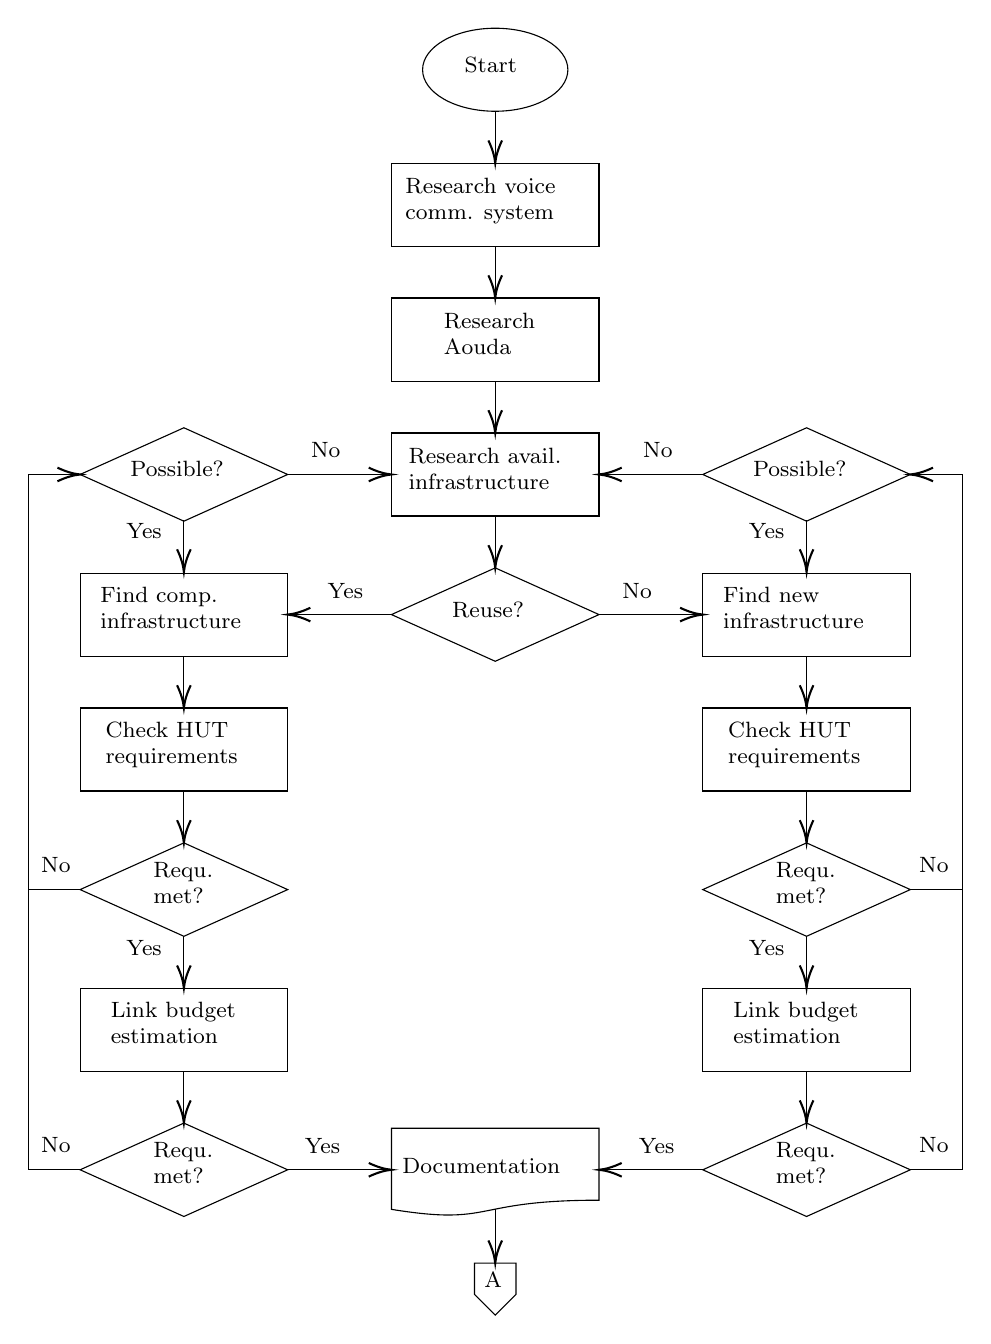
\begin{tikzpicture}[x=0.75pt,y=0.75pt,yscale=-1,xscale=1]
%uncomment if require: \path (0,667); %set diagram left start at 0, and has height of 667

%Shape: Diamond [id:dp04084543344377911] 
\draw   (145,202.5) -- (195,225) -- (145,247.5) -- (95,225) -- cycle ;
%Straight Lines [id:da3172337098532787] 
\draw    (243,225) -- (195,225) ;
\draw [shift={(245,225)}, rotate = 180] [color={rgb, 255:red, 0; green, 0; blue, 0 }  ][line width=0.75]    (10.93,-3.29) .. controls (6.95,-1.4) and (3.31,-0.3) .. (0,0) .. controls (3.31,0.3) and (6.95,1.4) .. (10.93,3.29)   ;

%Shape: Ellipse [id:dp5174120932429653] 
\draw   (260,30) .. controls (260,18.95) and (275.67,10) .. (295,10) .. controls (314.33,10) and (330,18.95) .. (330,30) .. controls (330,41.05) and (314.33,50) .. (295,50) .. controls (275.67,50) and (260,41.05) .. (260,30) -- cycle ;

%Straight Lines [id:da5375994326166968] 
\draw    (295,115) -- (295,138) ;
\draw [shift={(295,140)}, rotate = 270] [color={rgb, 255:red, 0; green, 0; blue, 0 }  ][line width=0.75]    (10.93,-3.29) .. controls (6.95,-1.4) and (3.31,-0.3) .. (0,0) .. controls (3.31,0.3) and (6.95,1.4) .. (10.93,3.29)   ;
%Shape: Rectangle [id:dp32571227246524637] 
\draw   (245,140) -- (345,140) -- (345,180) -- (245,180) -- cycle ;

%Straight Lines [id:da7335469832694597] 
\draw    (295,180) -- (295,203) ;
\draw [shift={(295,205)}, rotate = 270] [color={rgb, 255:red, 0; green, 0; blue, 0 }  ][line width=0.75]    (10.93,-3.29) .. controls (6.95,-1.4) and (3.31,-0.3) .. (0,0) .. controls (3.31,0.3) and (6.95,1.4) .. (10.93,3.29)   ;
%Shape: Rectangle [id:dp18134004375921853] 
\draw   (245,205) -- (345,205) -- (345,245) -- (245,245) -- cycle ;

%Shape: Diamond [id:dp07434166202435644] 
\draw   (295,270) -- (345,292.5) -- (295,315) -- (245,292.5) -- cycle ;

%Straight Lines [id:da48336252424104975] 
\draw    (295,245) -- (295,268) ;
\draw [shift={(295,270)}, rotate = 270] [color={rgb, 255:red, 0; green, 0; blue, 0 }  ][line width=0.75]    (10.93,-3.29) .. controls (6.95,-1.4) and (3.31,-0.3) .. (0,0) .. controls (3.31,0.3) and (6.95,1.4) .. (10.93,3.29)   ;
%Shape: Rectangle [id:dp2129984339344504] 
\draw   (95,272.5) -- (195,272.5) -- (195,312.5) -- (95,312.5) -- cycle ;

%Straight Lines [id:da30600129254949016] 
\draw    (245,292.5) -- (197,292.5) ;
\draw [shift={(195,292.5)}, rotate = 360] [color={rgb, 255:red, 0; green, 0; blue, 0 }  ][line width=0.75]    (10.93,-3.29) .. controls (6.95,-1.4) and (3.31,-0.3) .. (0,0) .. controls (3.31,0.3) and (6.95,1.4) .. (10.93,3.29)   ;

%Shape: Rectangle [id:dp9927955770991572] 
\draw   (395,272.5) -- (495,272.5) -- (495,312.5) -- (395,312.5) -- cycle ;

%Straight Lines [id:da9340236776856534] 
\draw    (393,292.5) -- (345,292.5) ;
\draw [shift={(395,292.5)}, rotate = 180] [color={rgb, 255:red, 0; green, 0; blue, 0 }  ][line width=0.75]    (10.93,-3.29) .. controls (6.95,-1.4) and (3.31,-0.3) .. (0,0) .. controls (3.31,0.3) and (6.95,1.4) .. (10.93,3.29)   ;

%Shape: Rectangle [id:dp37011622873973793] 
\draw   (95,472.5) -- (195,472.5) -- (195,512.5) -- (95,512.5) -- cycle ;

%Straight Lines [id:da38599765543397413] 
\draw    (145,312.5) -- (145,335.5) ;
\draw [shift={(145,337.5)}, rotate = 270] [color={rgb, 255:red, 0; green, 0; blue, 0 }  ][line width=0.75]    (10.93,-3.29) .. controls (6.95,-1.4) and (3.31,-0.3) .. (0,0) .. controls (3.31,0.3) and (6.95,1.4) .. (10.93,3.29)   ;
%Shape: Diamond [id:dp40266300634290997] 
\draw   (145,402.5) -- (195,425) -- (145,447.5) -- (95,425) -- cycle ;

%Shape: Rectangle [id:dp19725156714424963] 
\draw   (95,337.5) -- (195,337.5) -- (195,377.5) -- (95,377.5) -- cycle ;
%Straight Lines [id:da8143450822524205] 
\draw    (145,377.5) -- (145,400.5) ;
\draw [shift={(145,402.5)}, rotate = 270] [color={rgb, 255:red, 0; green, 0; blue, 0 }  ][line width=0.75]    (10.93,-3.29) .. controls (6.95,-1.4) and (3.31,-0.3) .. (0,0) .. controls (3.31,0.3) and (6.95,1.4) .. (10.93,3.29)   ;
%Straight Lines [id:da2732080381707884] 
\draw    (145,447.5) -- (145,470.5) ;
\draw [shift={(145,472.5)}, rotate = 270] [color={rgb, 255:red, 0; green, 0; blue, 0 }  ][line width=0.75]    (10.93,-3.29) .. controls (6.95,-1.4) and (3.31,-0.3) .. (0,0) .. controls (3.31,0.3) and (6.95,1.4) .. (10.93,3.29)   ;

%Straight Lines [id:da3006343778538556] 
\draw    (70,425) -- (95,425) ;
%Straight Lines [id:da8915158079209304] 
\draw    (70,225) -- (70,425) ;
%Shape: Diamond [id:dp383009228365645] 
\draw   (145,537.5) -- (195,560) -- (145,582.5) -- (95,560) -- cycle ;

%Straight Lines [id:da5536604029887944] 
\draw    (145,512.5) -- (145,535.5) ;
\draw [shift={(145,537.5)}, rotate = 270] [color={rgb, 255:red, 0; green, 0; blue, 0 }  ][line width=0.75]    (10.93,-3.29) .. controls (6.95,-1.4) and (3.31,-0.3) .. (0,0) .. controls (3.31,0.3) and (6.95,1.4) .. (10.93,3.29)   ;
%Straight Lines [id:da4533379000087212] 
\draw    (70,560) -- (95,560) ;
%Straight Lines [id:da6765632118654783] 
\draw    (70,425) -- (70,560) ;
%Straight Lines [id:da2521838515704664] 
\draw    (243,560) -- (195,560) ;
\draw [shift={(245,560)}, rotate = 180] [color={rgb, 255:red, 0; green, 0; blue, 0 }  ][line width=0.75]    (10.93,-3.29) .. controls (6.95,-1.4) and (3.31,-0.3) .. (0,0) .. controls (3.31,0.3) and (6.95,1.4) .. (10.93,3.29)   ;

%Shape: Rectangle [id:dp12448173161359821] 
\draw   (245,75) -- (345,75) -- (345,115) -- (245,115) -- cycle ;

%Straight Lines [id:da9099441526360148] 
\draw    (295,50) -- (295,73) ;
\draw [shift={(295,75)}, rotate = 270] [color={rgb, 255:red, 0; green, 0; blue, 0 }  ][line width=0.75]    (10.93,-3.29) .. controls (6.95,-1.4) and (3.31,-0.3) .. (0,0) .. controls (3.31,0.3) and (6.95,1.4) .. (10.93,3.29)   ;
%Flowchart: Document [id:dp8581842881262494] 
\draw   (245,540) -- (345,540) -- (345,574.65) .. controls (282.5,574.65) and (295,587.15) .. (245,579.06) -- cycle ;

%Straight Lines [id:da5600223852016903] 
\draw    (295,579) -- (295,603) ;
\draw [shift={(295,605)}, rotate = 270] [color={rgb, 255:red, 0; green, 0; blue, 0 }  ][line width=0.75]    (10.93,-3.29) .. controls (6.95,-1.4) and (3.31,-0.3) .. (0,0) .. controls (3.31,0.3) and (6.95,1.4) .. (10.93,3.29)   ;

%Shape: Rectangle [id:dp3333038890792923] 
\draw   (395,472.5) -- (495,472.5) -- (495,512.5) -- (395,512.5) -- cycle ;

%Straight Lines [id:da9438938465543254] 
\draw    (445,312.5) -- (445,335.5) ;
\draw [shift={(445,337.5)}, rotate = 270] [color={rgb, 255:red, 0; green, 0; blue, 0 }  ][line width=0.75]    (10.93,-3.29) .. controls (6.95,-1.4) and (3.31,-0.3) .. (0,0) .. controls (3.31,0.3) and (6.95,1.4) .. (10.93,3.29)   ;
%Shape: Diamond [id:dp9985955236044979] 
\draw   (445,402.5) -- (495,425) -- (445,447.5) -- (395,425) -- cycle ;

%Shape: Rectangle [id:dp2854078391107553] 
\draw   (395,337.5) -- (495,337.5) -- (495,377.5) -- (395,377.5) -- cycle ;
%Straight Lines [id:da1584499639924284] 
\draw    (445,377.5) -- (445,400.5) ;
\draw [shift={(445,402.5)}, rotate = 270] [color={rgb, 255:red, 0; green, 0; blue, 0 }  ][line width=0.75]    (10.93,-3.29) .. controls (6.95,-1.4) and (3.31,-0.3) .. (0,0) .. controls (3.31,0.3) and (6.95,1.4) .. (10.93,3.29)   ;
%Straight Lines [id:da5667295278418567] 
\draw    (445,447.5) -- (445,470.5) ;
\draw [shift={(445,472.5)}, rotate = 270] [color={rgb, 255:red, 0; green, 0; blue, 0 }  ][line width=0.75]    (10.93,-3.29) .. controls (6.95,-1.4) and (3.31,-0.3) .. (0,0) .. controls (3.31,0.3) and (6.95,1.4) .. (10.93,3.29)   ;

%Shape: Diamond [id:dp5343458308272999] 
\draw   (445,537.5) -- (495,560) -- (445,582.5) -- (395,560) -- cycle ;

%Straight Lines [id:da1086789531244099] 
\draw    (445,512.5) -- (445,535.5) ;
\draw [shift={(445,537.5)}, rotate = 270] [color={rgb, 255:red, 0; green, 0; blue, 0 }  ][line width=0.75]    (10.93,-3.29) .. controls (6.95,-1.4) and (3.31,-0.3) .. (0,0) .. controls (3.31,0.3) and (6.95,1.4) .. (10.93,3.29)   ;

%Straight Lines [id:da9693296657056982] 
\draw    (520,425) -- (495,425) ;
%Straight Lines [id:da45205438987238056] 
\draw    (520,225) -- (520,425) ;
%Straight Lines [id:da7322252024595366] 
\draw    (520,560) -- (495,560) ;
%Straight Lines [id:da01728937619143922] 
\draw    (520,425) -- (520,560) ;
%Straight Lines [id:da06866089729387759] 
\draw    (395,560) -- (347,560) ;
\draw [shift={(345,560)}, rotate = 360] [color={rgb, 255:red, 0; green, 0; blue, 0 }  ][line width=0.75]    (10.93,-3.29) .. controls (6.95,-1.4) and (3.31,-0.3) .. (0,0) .. controls (3.31,0.3) and (6.95,1.4) .. (10.93,3.29)   ;

%Pentagon Arrow [id:dp7793829288673029] 
\draw   (305,605) -- (305,620) -- (295,630) -- (285,620) -- (285,605) -- cycle ;
%Straight Lines [id:da03300375168213554] 
\draw    (70,225) -- (93,225) ;
\draw [shift={(95,225)}, rotate = 180] [color={rgb, 255:red, 0; green, 0; blue, 0 }  ][line width=0.75]    (10.93,-3.29) .. controls (6.95,-1.4) and (3.31,-0.3) .. (0,0) .. controls (3.31,0.3) and (6.95,1.4) .. (10.93,3.29)   ;
%Straight Lines [id:da3427925512939771] 
\draw    (145,247) -- (145,270) ;
\draw [shift={(145,272)}, rotate = 270] [color={rgb, 255:red, 0; green, 0; blue, 0 }  ][line width=0.75]    (10.93,-3.29) .. controls (6.95,-1.4) and (3.31,-0.3) .. (0,0) .. controls (3.31,0.3) and (6.95,1.4) .. (10.93,3.29)   ;

%Shape: Diamond [id:dp7243204751627801] 
\draw   (445,202.5) -- (495,225) -- (445,247.5) -- (395,225) -- cycle ;
%Straight Lines [id:da511170422936666] 
\draw    (395,225) -- (347,225) ;
\draw [shift={(345,225)}, rotate = 360] [color={rgb, 255:red, 0; green, 0; blue, 0 }  ][line width=0.75]    (10.93,-3.29) .. controls (6.95,-1.4) and (3.31,-0.3) .. (0,0) .. controls (3.31,0.3) and (6.95,1.4) .. (10.93,3.29)   ;
%Straight Lines [id:da9511402424924598] 
\draw    (445,247) -- (445,270) ;
\draw [shift={(445,272)}, rotate = 270] [color={rgb, 255:red, 0; green, 0; blue, 0 }  ][line width=0.75]    (10.93,-3.29) .. controls (6.95,-1.4) and (3.31,-0.3) .. (0,0) .. controls (3.31,0.3) and (6.95,1.4) .. (10.93,3.29)   ;

%Straight Lines [id:da8219755692109167] 
\draw    (497,225) -- (520,225) ;
\draw [shift={(495,225)}, rotate = 0] [color={rgb, 255:red, 0; green, 0; blue, 0 }  ][line width=0.75]    (10.93,-3.29) .. controls (6.95,-1.4) and (3.31,-0.3) .. (0,0) .. controls (3.31,0.3) and (6.95,1.4) .. (10.93,3.29)   ;

% Text Node
\draw (279,23) node [anchor=north west][inner sep=0.75pt]  [font=\footnotesize] [align=left] {Start};
% Text Node
\draw (269,146) node [anchor=north west][inner sep=0.75pt]  [font=\footnotesize] [align=left] {Research\\Aouda};
% Text Node
\draw (252,211) node [anchor=north west][inner sep=0.75pt]  [font=\footnotesize] [align=left] {Research avail.\\infrastructure};
% Text Node
\draw (273,285) node [anchor=north west][inner sep=0.75pt]  [font=\footnotesize] [align=left] {Reuse?};
% Text Node
\draw (103.5,278) node [anchor=north west][inner sep=0.75pt]  [font=\footnotesize] [align=left] {Find comp.\\infrastructure};
% Text Node
\draw (403.5,278) node [anchor=north west][inner sep=0.75pt]  [font=\footnotesize] [align=left] {Find new\\infrastructure};
% Text Node
\draw (213,276) node [anchor=north west][inner sep=0.75pt]  [font=\footnotesize] [align=left] {Yes};
% Text Node
\draw (355,276) node [anchor=north west][inner sep=0.75pt]  [font=\footnotesize] [align=left] {No};
% Text Node
\draw (108.5,478) node [anchor=north west][inner sep=0.75pt]  [font=\footnotesize] [align=left] {Link budget\\estimation};
% Text Node
\draw (129,410.5) node [anchor=north west][inner sep=0.75pt]  [font=\footnotesize] [align=left] {Requ.\\met?};
% Text Node
\draw (106,343) node [anchor=north west][inner sep=0.75pt]  [font=\footnotesize] [align=left] {Check HUT\\requirements};
% Text Node
\draw (116,448) node [anchor=north west][inner sep=0.75pt]  [font=\footnotesize] [align=left] {Yes};
% Text Node
\draw (129,545.5) node [anchor=north west][inner sep=0.75pt]  [font=\footnotesize] [align=left] {Requ.\\met?};
% Text Node
\draw (75,543) node [anchor=north west][inner sep=0.75pt]  [font=\footnotesize] [align=left] {No};
% Text Node
\draw (250.5,81) node [anchor=north west][inner sep=0.75pt]  [font=\footnotesize] [align=left] {Research voice\\comm. system};
% Text Node
\draw (249,553) node [anchor=north west][inner sep=0.75pt]  [font=\footnotesize] [align=left] {Documentation};
% Text Node
\draw (202,543.5) node [anchor=north west][inner sep=0.75pt]  [font=\footnotesize] [align=left] {Yes};
% Text Node
\draw (429,545.5) node [anchor=north west][inner sep=0.75pt]  [font=\footnotesize] [align=left] {Requ.\\met?};
% Text Node
\draw (416,448) node [anchor=north west][inner sep=0.75pt]  [font=\footnotesize] [align=left] {Yes};
% Text Node
\draw (429,410.5) node [anchor=north west][inner sep=0.75pt]  [font=\footnotesize] [align=left] {Requ.\\met?};
% Text Node
\draw (408.5,478) node [anchor=north west][inner sep=0.75pt]  [font=\footnotesize] [align=left] {Link budget\\estimation};
% Text Node
\draw (406,343) node [anchor=north west][inner sep=0.75pt]  [font=\footnotesize] [align=left] {Check HUT\\requirements};
% Text Node
\draw (363,543.5) node [anchor=north west][inner sep=0.75pt]  [font=\footnotesize] [align=left] {Yes};
% Text Node
\draw (288.5,608) node [anchor=north west][inner sep=0.75pt]  [font=\footnotesize] [align=left] {A};
% Text Node
\draw (498,543) node [anchor=north west][inner sep=0.75pt]  [font=\footnotesize] [align=left] {No};
% Text Node
\draw (498,408) node [anchor=north west][inner sep=0.75pt]  [font=\footnotesize] [align=left] {No};
% Text Node
\draw (75,408) node [anchor=north west][inner sep=0.75pt]  [font=\footnotesize] [align=left] {No};
% Text Node
\draw (205,208.5) node [anchor=north west][inner sep=0.75pt]  [font=\footnotesize] [align=left] {No};
% Text Node
\draw (118,217.5) node [anchor=north west][inner sep=0.75pt]  [font=\footnotesize] [align=left] {Possible?};
% Text Node
\draw (116,247.5) node [anchor=north west][inner sep=0.75pt]  [font=\footnotesize] [align=left] {Yes};
% Text Node
\draw (418,217.5) node [anchor=north west][inner sep=0.75pt]  [font=\footnotesize] [align=left] {Possible?};
% Text Node
\draw (416,247.5) node [anchor=north west][inner sep=0.75pt]  [font=\footnotesize] [align=left] {Yes};
% Text Node
\draw (365,208.5) node [anchor=north west][inner sep=0.75pt]  [font=\footnotesize] [align=left] {No};


\end{tikzpicture}

	\caption{Part one of the flowchart of this thesis. It illustartes which steps were taken in order to achieve the deliverables.}
	\label{fig:tikz_flowchart_1}
\end{figure}
\begin{figure}[h!]
	\centering
	

\tikzset{every picture/.style={line width=0.75pt}} %set default line width to 0.75pt        

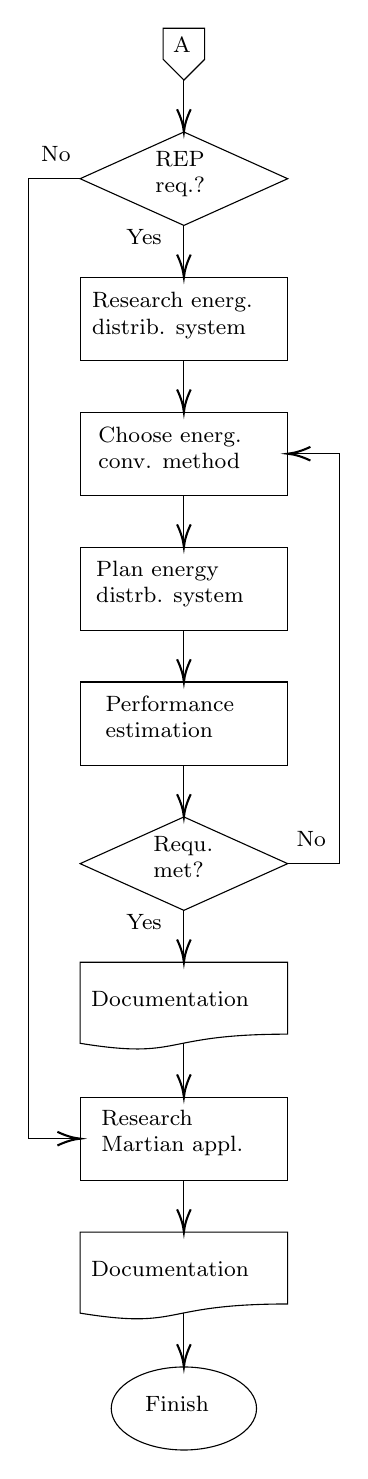
\begin{tikzpicture}[x=0.75pt,y=0.75pt,yscale=-1,xscale=1]
%uncomment if require: \path (0,882); %set diagram left start at 0, and has height of 882

%Pentagon Arrow [id:dp6295335837224703] 
\draw   (365,45) -- (365,60) -- (355,70) -- (345,60) -- (345,45) -- cycle ;

%Shape: Rectangle [id:dp9114846783986272] 
\draw   (305,165) -- (405,165) -- (405,205) -- (305,205) -- cycle ;

%Straight Lines [id:da1841951473424126] 
\draw    (355,70) -- (355,93) ;
\draw [shift={(355,95)}, rotate = 270] [color={rgb, 255:red, 0; green, 0; blue, 0 }  ][line width=0.75]    (10.93,-3.29) .. controls (6.95,-1.4) and (3.31,-0.3) .. (0,0) .. controls (3.31,0.3) and (6.95,1.4) .. (10.93,3.29)   ;
%Shape: Diamond [id:dp3275955259803509] 
\draw   (355,95) -- (405,117.5) -- (355,140) -- (305,117.5) -- cycle ;
%Straight Lines [id:da6311173750553984] 
\draw    (355,140) -- (355,163) ;
\draw [shift={(355,165)}, rotate = 270] [color={rgb, 255:red, 0; green, 0; blue, 0 }  ][line width=0.75]    (10.93,-3.29) .. controls (6.95,-1.4) and (3.31,-0.3) .. (0,0) .. controls (3.31,0.3) and (6.95,1.4) .. (10.93,3.29)   ;

%Shape: Rectangle [id:dp913835377980921] 
\draw   (305,230) -- (405,230) -- (405,270) -- (305,270) -- cycle ;

%Straight Lines [id:da3649991025923325] 
\draw    (355,205) -- (355,228) ;
\draw [shift={(355,230)}, rotate = 270] [color={rgb, 255:red, 0; green, 0; blue, 0 }  ][line width=0.75]    (10.93,-3.29) .. controls (6.95,-1.4) and (3.31,-0.3) .. (0,0) .. controls (3.31,0.3) and (6.95,1.4) .. (10.93,3.29)   ;
%Straight Lines [id:da43992652550284816] 
\draw    (355,270) -- (355,293) ;
\draw [shift={(355,295)}, rotate = 270] [color={rgb, 255:red, 0; green, 0; blue, 0 }  ][line width=0.75]    (10.93,-3.29) .. controls (6.95,-1.4) and (3.31,-0.3) .. (0,0) .. controls (3.31,0.3) and (6.95,1.4) .. (10.93,3.29)   ;
%Shape: Rectangle [id:dp9403171441896898] 
\draw   (305,295) -- (405,295) -- (405,335) -- (305,335) -- cycle ;

%Shape: Rectangle [id:dp553852729933479] 
\draw   (305,360) -- (405,360) -- (405,400) -- (305,400) -- cycle ;
%Straight Lines [id:da1550632508471741] 
\draw    (355,335) -- (355,358) ;
\draw [shift={(355,360)}, rotate = 270] [color={rgb, 255:red, 0; green, 0; blue, 0 }  ][line width=0.75]    (10.93,-3.29) .. controls (6.95,-1.4) and (3.31,-0.3) .. (0,0) .. controls (3.31,0.3) and (6.95,1.4) .. (10.93,3.29)   ;
%Straight Lines [id:da1341632742496266] 
\draw    (355,400) -- (355,423) ;
\draw [shift={(355,425)}, rotate = 270] [color={rgb, 255:red, 0; green, 0; blue, 0 }  ][line width=0.75]    (10.93,-3.29) .. controls (6.95,-1.4) and (3.31,-0.3) .. (0,0) .. controls (3.31,0.3) and (6.95,1.4) .. (10.93,3.29)   ;
%Shape: Diamond [id:dp8080302672223327] 
\draw   (355,425) -- (405,447.5) -- (355,470) -- (305,447.5) -- cycle ;

%Straight Lines [id:da3135121459732009] 
\draw    (407,250) -- (430,250) ;
\draw [shift={(405,250)}, rotate = 0] [color={rgb, 255:red, 0; green, 0; blue, 0 }  ][line width=0.75]    (10.93,-3.29) .. controls (6.95,-1.4) and (3.31,-0.3) .. (0,0) .. controls (3.31,0.3) and (6.95,1.4) .. (10.93,3.29)   ;
%Straight Lines [id:da1661173997317298] 
\draw    (430,250) -- (430,447.5) ;
%Straight Lines [id:da013009727986448727] 
\draw    (430,447.5) -- (405,447.5) ;

%Straight Lines [id:da8133901261188266] 
\draw    (355,470) -- (355,493) ;
\draw [shift={(355,495)}, rotate = 270] [color={rgb, 255:red, 0; green, 0; blue, 0 }  ][line width=0.75]    (10.93,-3.29) .. controls (6.95,-1.4) and (3.31,-0.3) .. (0,0) .. controls (3.31,0.3) and (6.95,1.4) .. (10.93,3.29)   ;

%Flowchart: Document [id:dp6420835715080364] 
\draw   (305,495) -- (405,495) -- (405,529.65) .. controls (342.5,529.65) and (355,542.15) .. (305,534.06) -- cycle ;

%Straight Lines [id:da3287541689868827] 
\draw    (355,534) -- (355,558) ;
\draw [shift={(355,560)}, rotate = 270] [color={rgb, 255:red, 0; green, 0; blue, 0 }  ][line width=0.75]    (10.93,-3.29) .. controls (6.95,-1.4) and (3.31,-0.3) .. (0,0) .. controls (3.31,0.3) and (6.95,1.4) .. (10.93,3.29)   ;

%Shape: Rectangle [id:dp9760404082725573] 
\draw   (305,560) -- (405,560) -- (405,600) -- (305,600) -- cycle ;
%Flowchart: Document [id:dp2517134736579656] 
\draw   (305,625) -- (405,625) -- (405,659.65) .. controls (342.5,659.65) and (355,672.15) .. (305,664.06) -- cycle ;

%Straight Lines [id:da5089558784451147] 
\draw    (355,664) -- (355,688) ;
\draw [shift={(355,690)}, rotate = 270] [color={rgb, 255:red, 0; green, 0; blue, 0 }  ][line width=0.75]    (10.93,-3.29) .. controls (6.95,-1.4) and (3.31,-0.3) .. (0,0) .. controls (3.31,0.3) and (6.95,1.4) .. (10.93,3.29)   ;

%Straight Lines [id:da19223774212748634] 
\draw    (355,600) -- (355,623) ;
\draw [shift={(355,625)}, rotate = 270] [color={rgb, 255:red, 0; green, 0; blue, 0 }  ][line width=0.75]    (10.93,-3.29) .. controls (6.95,-1.4) and (3.31,-0.3) .. (0,0) .. controls (3.31,0.3) and (6.95,1.4) .. (10.93,3.29)   ;
%Straight Lines [id:da9396270466808674] 
\draw    (280,580) -- (303,580) ;
\draw [shift={(305,580)}, rotate = 180] [color={rgb, 255:red, 0; green, 0; blue, 0 }  ][line width=0.75]    (10.93,-3.29) .. controls (6.95,-1.4) and (3.31,-0.3) .. (0,0) .. controls (3.31,0.3) and (6.95,1.4) .. (10.93,3.29)   ;
%Straight Lines [id:da020572157364605825] 
\draw    (280,117.5) -- (305,117.5) ;

%Straight Lines [id:da680181864059918] 
\draw    (280,117.5) -- (280,580) ;
%Shape: Ellipse [id:dp16223416818247482] 
\draw   (320,710) .. controls (320,698.95) and (335.67,690) .. (355,690) .. controls (374.33,690) and (390,698.95) .. (390,710) .. controls (390,721.05) and (374.33,730) .. (355,730) .. controls (335.67,730) and (320,721.05) .. (320,710) -- cycle ;

% Text Node
\draw (348.5,48) node [anchor=north west][inner sep=0.75pt]  [font=\footnotesize] [align=left] {A};
% Text Node
\draw (309.5,171) node [anchor=north west][inner sep=0.75pt]  [font=\footnotesize] [align=left] {Research energ.\\distrib. system};
% Text Node
\draw (340,103) node [anchor=north west][inner sep=0.75pt]  [font=\footnotesize] [align=left] {REP\\req.?};
% Text Node
\draw (326,140.5) node [anchor=north west][inner sep=0.75pt]  [font=\footnotesize] [align=left] {Yes};
% Text Node
\draw (312.5,236) node [anchor=north west][inner sep=0.75pt]  [font=\footnotesize] [align=left] {Choose energ.\\conv. method};
% Text Node
\draw (311.5,300.5) node [anchor=north west][inner sep=0.75pt]  [font=\footnotesize] [align=left] {Plan energy\\distrb. system};
% Text Node
\draw (316,365.5) node [anchor=north west][inner sep=0.75pt]  [font=\footnotesize] [align=left] {Performance\\estimation};
% Text Node
\draw (339,433) node [anchor=north west][inner sep=0.75pt]  [font=\footnotesize] [align=left] {Requ.\\met?};
% Text Node
\draw (408,430.5) node [anchor=north west][inner sep=0.75pt]  [font=\footnotesize] [align=left] {No};
% Text Node
\draw (326,470.5) node [anchor=north west][inner sep=0.75pt]  [font=\footnotesize] [align=left] {Yes};
% Text Node
\draw (309,508) node [anchor=north west][inner sep=0.75pt]  [font=\footnotesize] [align=left] {Documentation};
% Text Node
\draw (314,565) node [anchor=north west][inner sep=0.75pt]  [font=\footnotesize] [align=left] {Research\\Martian appl.};
% Text Node
\draw (309,638) node [anchor=north west][inner sep=0.75pt]  [font=\footnotesize] [align=left] {Documentation};
% Text Node
\draw (285,100.5) node [anchor=north west][inner sep=0.75pt]  [font=\footnotesize] [align=left] {No};
% Text Node
\draw (335,703) node [anchor=north west][inner sep=0.75pt]  [font=\footnotesize] [align=left] {Finish};


\end{tikzpicture}

	\caption{Part two of the flowchart of this thesis. It illustartes which steps were taken in order to achieve the deliverables.}
	\label{fig:tikz_flowchart_2}
\end{figure}

\subsection{Thesis Structure}
The first part of this thesis contains the \textbf{Methodology} in which the mathematical fundamentals for the system design and the performance estimations of the self-sufficient energy distribution and the voice communication system are explained. This is followed by the \textbf{Results}, presenting the system design and the results of the performance estimations. Finally, the \textbf{Conclusion and critical reflecion} summarizes and interprets the results and provides a critical reflection of this thesis. The appendices contain information about the OeWF and the Serenity spacesuit simulator, mathematical basics and the developed \MATLAB simulation for the performance estimation of the self-sufficient energy distribution system.


\chapter{Methodology}
In the following sections, the basics of electrical energy distribution and telecommunications necessary for this project are discussed. Since the self-sufficient voice communication system is being developed for use in Mars analog regions on Earth, the focus is on developing a model so that the use of the system in said regions can be simulated. The simulation results are then used to verify the designed system and therefore the requirements. At the end of each section it will be discussed how the developed model of the surface bound communication system on Earth has to be adapted, so that it can be used on the Martian surface instead.

\section{Electrical energy distribution} \label{sec:methodology}
A self-sufficient voice communication system constist of at least one or more electrical consumers that must be supplied with electrical energy. This requires a close examination of the system's electrical energy distribution, which includes an energy source, the energy conversion with a suitable electrical generator, internal electrical energy losses and -- if necessary -- an electrical energy storage device.

The decision to design a self-sufficient voice communication system was made due to a number of reasons. First, it makes the system independent of its location. This of course only applies if the system is operated in a location where there is a source of energy that can be converted by its electrical generator. As a result, it can operate without any external electrical energy source, which offers independence from a local power grid or other on-site electrical generators, such as fuel combustion generators.\footnote{During some of their previous missions the OeWF used diesel generators at the base camp to supply electrical consumers.} 

This already leads to the second and third reason regarding the environmentally harmful way in which electrical energy is generated by burning fossil fuels and the impracticality of fuel combustion generators. With consideration for the planet Earth and its sensitive ecosystem, as well as for future generations, the technologies available today must be used in such a way that the environmental impact of the use of the voice communication system is minimal. Furthermore, looking ahead to future Mars missions, the third reason arises from the fact that its just not a feasable option to bring fuel combustion generators -- and the infrastructure required -- to the Martian surface \cite{Bertol:2011, Mertens:2015}.  

Based on these reasons it was decided to supply the self-sufficient voice communication system from renewable energy sources, such as wind energy, hydroelectric energy, solar energy, bioenergy from biomass, tidal energy etc. Hydroelectric and tidal energy were quickly disregarded because there are no bodies of water on the Martian surface. And since the OeWF conducts Mars analog missions on Earth it is not likely that simulation will take place in locations where there are bodies of water that could provide these sources of energy. Bioenergy from biomass can be disregarded due to similar reasons. 

\section{Wind energy}
A brief investigation of wind energy showed that the \emph{mechanical rotor power} $P_{\mathrm R} = \mathrm{d} T_{\mathrm W}/\mathrm{d} t$ in $\left(\mathrm W \right)$ can be determinerd from the time derivative of the kinetic energy $T_{\mathrm W}$ in $\left(\mathrm{Wh} \right)$ of a flowing gas -- which makes up the atmosphere of a planet and is also known as wind -- with the \emph{mass} $m_{\mathrm {gas}}$ in $\left(\mathrm{kg} \right)$, the uniform and constant \emph{flow velocity} $v_{\mathrm W}$ in $\left(\mathrm{m} \mathrm{s^{-1}}\right)$, the \emph{density} near the ground\footnote{This only applies if the change in gas density at the height of the rotors of the wind turbine is negligible compared to the ground.} $\varrho_{\mathrm {gas}}$ in $\left(\mathrm{kg} \mathrm{m}^{-3}\right)$, the \emph{rotor radius} $r_{\mathrm{R}}$ in $\left(\mathrm{m}\right)$ and the \emph{performance coefficient}\footnote{Modern wind turbines reach a performance coefficient ranging from $0,35$ to $0,45$. According to Betz's law, the ideal perfomance coefficient is $0,5926$.} $c_{\mathrm P}$ in $\left( 1 \right)$. The area $A_\mathrm{W} = r_{\mathrm{R}}^2 \, \pi$ in $\left(\mathrm{m}^2 \right)$ must be perpendicular to the flowing gas. Taking into account the \emph{efficiency} of the mechanical transmission and the electrical generator $\eta_{\mathrm{mech}}$ in $\left( 1 \right)$, the \emph{generated electrical power} $P_{\mathrm{el}}$ in $\left(\mathrm W \right)$ can be calculated. A summary of this can be seen below \cite{Rebhan:2002, Flosdorff:2008, Hau:2016, Gawlik:2018}:
\begin{equation}
	\vcenter{\hbox{\begin{minipage}{.5\textwidth}
		\centering
		

\tikzset{every picture/.style={line width=0.75pt}} %set default line width to 0.75pt        

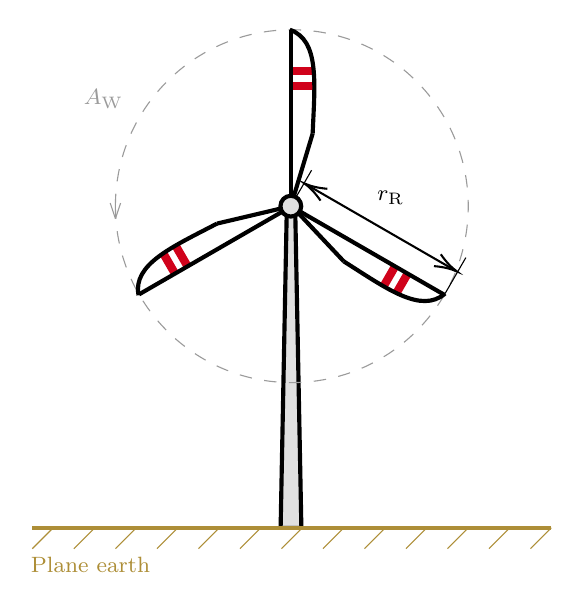
\begin{tikzpicture}[x=0.75pt,y=0.75pt,yscale=-1,xscale=1]
%uncomment if require: \path (0,345); %set diagram left start at 0, and has height of 345

%Straight Lines [id:da2855457278708555] 
\draw    (154.52,97.68) -- (144.52,115) ;
%Shape: Trapezoid [id:dp6563165495841363] 
\draw  [fill={rgb, 255:red, 224; green, 224; blue, 224 }  ,fill opacity=1 ][line width=1.5]  (139.6,270) -- (142.6,115) -- (146.6,115) -- (149.6,270) -- cycle ;
%Shape: Circle [id:dp4391264400751236] 
\draw  [color={rgb, 255:red, 155; green, 155; blue, 155 }  ,draw opacity=1 ][dash pattern={on 4.5pt off 4.5pt}] (60,115) .. controls (60,68.06) and (98.06,30) .. (145,30) .. controls (191.94,30) and (230,68.06) .. (230,115) .. controls (230,161.94) and (191.94,200) .. (145,200) .. controls (98.06,200) and (60,161.94) .. (60,115) -- cycle ;
%Straight Lines [id:da2732716340606678] 
\draw [color={rgb, 255:red, 208; green, 2; blue, 27 }  ,draw opacity=1 ][line width=3]    (144.52,50) -- (155.52,50) ;
%Straight Lines [id:da3625566257672834] 
\draw [color={rgb, 255:red, 208; green, 2; blue, 27 }  ,draw opacity=1 ][line width=3]    (144.52,57) -- (155.52,57) ;
%Straight Lines [id:da3551490622606075] 
\draw [line width=1.5]    (144.52,30) -- (144.52,115) ;
%Curve Lines [id:da31858770163213945] 
\draw [line width=1.5]    (144.04,30) .. controls (158.54,35) and (156.02,56) .. (155.04,80) ;
%Straight Lines [id:da40134971489014015] 
\draw [line width=1.5]    (144.52,115) -- (155.04,80) ;
%Straight Lines [id:da6221475193546597] 
\draw [color={rgb, 255:red, 208; green, 2; blue, 27 }  ,draw opacity=1 ][line width=3]    (194.75,144) -- (189.25,153.53) ;
%Straight Lines [id:da46600729912444394] 
\draw [color={rgb, 255:red, 208; green, 2; blue, 27 }  ,draw opacity=1 ][line width=3]    (200.81,147.5) -- (195.31,157.03) ;
%Straight Lines [id:da24248073534191383] 
\draw [line width=1.5]    (218.13,157.5) -- (144.52,115) ;
%Curve Lines [id:da8105786474721348] 
\draw [line width=1.5]    (218.85,157.08) .. controls (207.27,167.14) and (190.35,154.46) .. (170.05,141.61) ;
%Straight Lines [id:da649738591055431] 
\draw [line width=1.5]    (145,115) -- (170.05,141.61) ;
%Straight Lines [id:da39570308318736713] 
\draw [color={rgb, 255:red, 208; green, 2; blue, 27 }  ,draw opacity=1 ][line width=3]    (88.71,147.5) -- (83.21,137.97) ;
%Straight Lines [id:da21160602066475165] 
\draw [color={rgb, 255:red, 208; green, 2; blue, 27 }  ,draw opacity=1 ][line width=3]    (94.77,144) -- (89.27,134.47) ;
%Straight Lines [id:da9797525004071665] 
\draw [line width=1.5]    (71.39,157.5) -- (145,115) ;
%Curve Lines [id:da9490200570005278] 
\draw [line width=1.5]    (71.15,157.92) .. controls (68.23,142.86) and (87.67,134.54) .. (108.95,123.39) ;
%Straight Lines [id:da6466154668803934] 
\draw [line width=1.5]    (144.52,115) -- (108.95,123.39) ;
%Shape: Circle [id:dp4546700879564365] 
\draw  [fill={rgb, 255:red, 224; green, 224; blue, 224 }  ,fill opacity=1 ][line width=1.5]  (139.52,115) .. controls (139.52,112.24) and (141.76,110) .. (144.52,110) .. controls (147.28,110) and (149.52,112.24) .. (149.52,115) .. controls (149.52,117.76) and (147.28,120) .. (144.52,120) .. controls (141.76,120) and (139.52,117.76) .. (139.52,115) -- cycle ;
%Straight Lines [id:da5512625411833432] 
\draw [color={rgb, 255:red, 173; green, 142; blue, 55 }  ,draw opacity=1 ][fill={rgb, 255:red, 139; green, 87; blue, 42 }  ,fill opacity=1 ][line width=1.5]    (20,270) -- (270,270) ;
%Straight Lines [id:da5304059380179822] 
\draw [color={rgb, 255:red, 173; green, 142; blue, 55 }  ,draw opacity=1 ]   (50,270) -- (40,280) ;
%Straight Lines [id:da3431793884624006] 
\draw [color={rgb, 255:red, 173; green, 142; blue, 55 }  ,draw opacity=1 ]   (70,270) -- (60,280) ;
%Straight Lines [id:da7136874676914755] 
\draw [color={rgb, 255:red, 173; green, 142; blue, 55 }  ,draw opacity=1 ]   (30,270) -- (20,280) ;
%Straight Lines [id:da21878729454445067] 
\draw [color={rgb, 255:red, 173; green, 142; blue, 55 }  ,draw opacity=1 ]   (90,270) -- (80,280) ;
%Straight Lines [id:da2119530108548371] 
\draw [color={rgb, 255:red, 173; green, 142; blue, 55 }  ,draw opacity=1 ]   (110,270) -- (100,280) ;
%Straight Lines [id:da9669600696257283] 
\draw [color={rgb, 255:red, 173; green, 142; blue, 55 }  ,draw opacity=1 ]   (130,270) -- (120,280) ;
%Straight Lines [id:da148721087656281] 
\draw [color={rgb, 255:red, 173; green, 142; blue, 55 }  ,draw opacity=1 ]   (150,270) -- (140,280) ;
%Straight Lines [id:da021478871305470992] 
\draw [color={rgb, 255:red, 173; green, 142; blue, 55 }  ,draw opacity=1 ]   (170,270) -- (160,280) ;
%Straight Lines [id:da6475678117315542] 
\draw [color={rgb, 255:red, 173; green, 142; blue, 55 }  ,draw opacity=1 ]   (190,270) -- (180,280) ;
%Straight Lines [id:da17413992256591215] 
\draw [color={rgb, 255:red, 173; green, 142; blue, 55 }  ,draw opacity=1 ]   (210,270) -- (200,280) ;
%Straight Lines [id:da3680869151900985] 
\draw [color={rgb, 255:red, 173; green, 142; blue, 55 }  ,draw opacity=1 ]   (230,270) -- (220,280) ;
%Straight Lines [id:da19438567917294902] 
\draw [color={rgb, 255:red, 173; green, 142; blue, 55 }  ,draw opacity=1 ]   (250,270) -- (240,280) ;
%Straight Lines [id:da0327170377597672] 
\draw [line width=0.75]    (222.88,145.5) -- (152.73,105) ;
\draw [shift={(151,104)}, rotate = 390] [color={rgb, 255:red, 0; green, 0; blue, 0 }  ][line width=0.75]    (10.93,-3.29) .. controls (6.95,-1.4) and (3.31,-0.3) .. (0,0) .. controls (3.31,0.3) and (6.95,1.4) .. (10.93,3.29)   ;
\draw [shift={(224.61,146.5)}, rotate = 210] [color={rgb, 255:red, 0; green, 0; blue, 0 }  ][line width=0.75]    (10.93,-3.29) .. controls (6.95,-1.4) and (3.31,-0.3) .. (0,0) .. controls (3.31,0.3) and (6.95,1.4) .. (10.93,3.29)   ;
%Straight Lines [id:da7589968423979443] 
\draw    (228.85,139.76) -- (218.85,157.08) ;
%Straight Lines [id:da015160365704311562] 
\draw [color={rgb, 255:red, 155; green, 155; blue, 155 }  ,draw opacity=1 ]   (60,121) -- (57.5,113.5) ;
%Straight Lines [id:da4975603923384009] 
\draw [color={rgb, 255:red, 155; green, 155; blue, 155 }  ,draw opacity=1 ]   (60,121) -- (62.5,113.5) ;

%Straight Lines [id:da5866655581447886] 
\draw [color={rgb, 255:red, 173; green, 142; blue, 55 }  ,draw opacity=1 ]   (270,270) -- (260,280) ;

% Text Node
\draw (185,106.4) node [anchor=north west][inner sep=0.75pt]  [font=\footnotesize]  {$r_{\mathrm{R}}$};
% Text Node
\draw (18,283) node [anchor=north west][inner sep=0.75pt]  [font=\footnotesize,color={rgb, 255:red, 173; green, 142; blue, 55 }  ,opacity=1 ] [align=left] {Plane earth};
% Text Node
\draw (43.5,57.4) node [anchor=north west][inner sep=0.75pt]  [font=\footnotesize,color={rgb, 255:red, 155; green, 155; blue, 155 }  ,opacity=1 ]  {$A_{\mathrm{W}}$};


\end{tikzpicture}

		\captionof{figure}{Turbine that converts kinetic energy from wind into electrical energy. The dashed circle represents the area $A_\mathrm{W}$ that is perpendicular to a flowing gas.}
	\end{minipage}}}
	\qquad\qquad
		\begin{gathered}
		T_{\mathrm W} = \frac{1}{2} \, m_{\mathrm {gas}} \, v_{\mathrm W}^2 \text{,}
		\\
		\vdots
		\\
		\dfrac{\mathrm{d} T_{\mathrm W}}{\mathrm{d} t} = \frac{c_{\mathrm P}}{2} \, \varrho_{\mathrm {gas}} \, v_{\mathrm W}^3 \, \underbrace{\pi \, r_{\mathrm{R}}^2}_{A_\mathrm{W}} \text{,}
		\\
		P_{\mathrm{el}} = \eta_{\mathrm{mech}} \, \dfrac{\mathrm{d} T_{\mathrm W}}{\mathrm{d} t} \text{.}
	\end{gathered}
\end{equation}

This method of converting electrical energy however, was rejected mainly due to the unpredictability of $v_{\mathrm W}$.\footnote{The direction from which the wind comes is irrelevant for most small-scale wind turbines, as they are rotatably mounted on a mast.} In order to bridge times when no wind blows, a large energy storage device would have to be required, which would be charged in times of strong wind. But due to the high acquisition costs of a large energy storage devices, and the relative short duration of the OeWF's missions, this approach is not practical. Another important aspect that led to the rejection of this method is the fact that mean wind speeds are highly dependent on the location and in most parts of the world, $10 \mathrm m$ above the ground, these are usually between $5 \mathrm m \mathrm s^{-1}$ to less than $2,5 \mathrm m \mathrm s^{-1}$ as shown in maps provided by \cite{Atlas:2020}. In addition it must be added, that the gas density of air on the Earth's surface $\varrho_{\mathrm {gas,E}} = 1,217 \mathrm{kg} \mathrm{m}^{-3}$ is a lot higher than the gas density on the Martian surface $\varrho_{\mathrm {gas,M}} \approx 0,020 \mathrm{kg}  \mathrm{m}^{-3}$ -- which is mainly made up of carbon dioxide $\left( \mathrm{CO}_2 \right)$ -- and that the wind speeds on Mars, measured by NASA's Viking Landers VL1 and VL2, range from $2 \mathrm m  \mathrm s^{-1}$ to $7 \mathrm m \mathrm s^{-1}$ during summer, $5 \mathrm m \mathrm s^{-1}$ to $10 \mathrm m \mathrm s^{-1}$ during fall and $17\mathrm m \mathrm s^{-1}$ to $30 \mathrm m  \mathrm s^{-1}$ during dust storms. It can therefore be seen that -- compared to Earth -- the greatest negative influnece on $P_{\mathrm R}$ is the density of the Martian atmosphere \cite{Grayzeck:2020, Williams:2020}.

\section{Solar energy} \label{sec:solar_energy}
The Sun constantly emits a \emph{radiation flux} of around $\Phi_{\mathrm{S}} = 3,845 \cdot 10^{26} \mathrm{W}$ into space. Without any doubt it is the greatest source of renewable energy in our solar system. To determine the \emph{solar irradiance} $E_\mathrm{S}$ in $\left( \mathrm{W} \mathrm{m}^{-2} \right)$ that arrives at the top of Earth's atmosphere, the mean distance between the Sun and Earth $r_{\mathrm{SE}} = 149,597870 \cdot 10^{6} \mathrm{km}$ -- which is often reffered to as \emph{astronomical unit} (AU) -- needs to be taken into account as shown in the equation (\ref{eq:e_sun}) \cite{Karttunen:2006, Bertol:2011, Mertens:2015, Wagner:2018}. 
	\begin{equation} \label{eq:e_sun}
	\centering
		E_{\mathrm{S}} = \frac{\Phi_{\mathrm{S}}}{4 \pi \, r_{\mathrm{SE}}^2} = \frac{3,845 \cdot 10^{26} \mathrm{W}}{4 \pi \cdot (1,49597870 \cdot 10^{11} \mathrm{m})^2} = 1367,21 \frac{\mathrm{W}}{\mathrm{m}^2}
	\end{equation}

Figure \ref{fig:tikz_angular_relationship} provides an illustration of the Sun and the Earth with consideration of the angular relationships, in which $\delta$ is the \emph{declination} of the Sun in $\left( ^\circ \right)$, $\varphi$ is the local \emph{latitude} of an observer on Earth in $\left( ^\circ \right)$ and $\gamma_{\mathrm{S}}$ is the \emph{altitude} of the Sun in $\left( ^\circ \right)$ at said latitude. The incident rays on the hemisphere facing the Sun (separated by the dashed line in figure \ref{fig:tikz_angular_relationship}) can be assumed to be parallel to each other due to the enormous distance between the Sun and Earth \cite{Landis:1995, Karttunen:2006, Mertens:2015, Wagner:2018}.
\begin{figure}[h!]
	\centering
	

\tikzset{every picture/.style={line width=0.75pt}} %set default line width to 0.75pt        

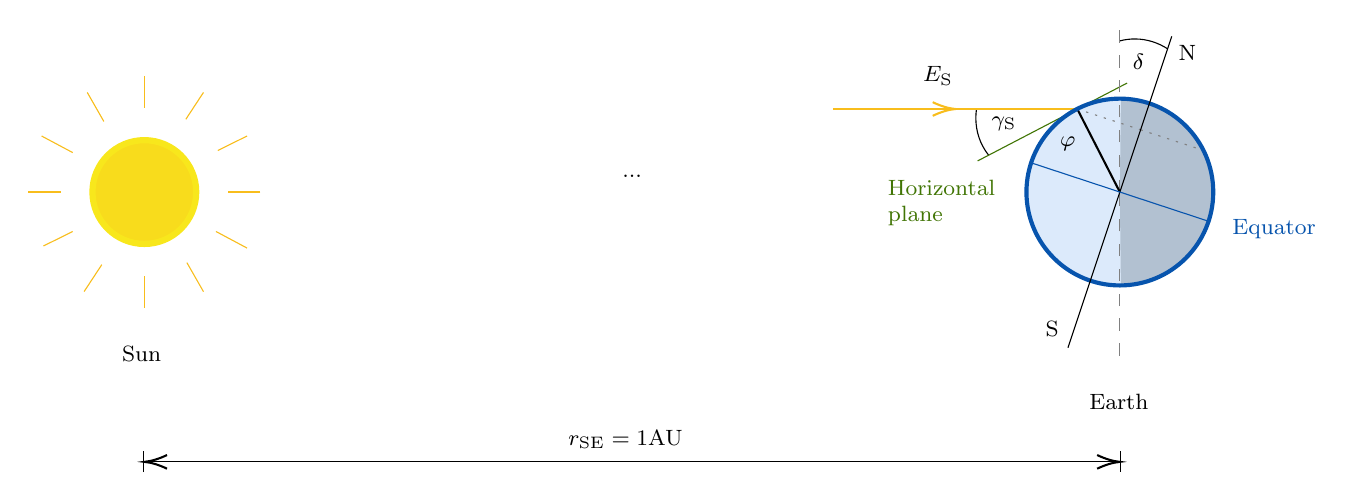
\begin{tikzpicture}[x=0.75pt,y=0.75pt,yscale=-1,xscale=1]
%uncomment if require: \path (0,447); %set diagram left start at 0, and has height of 447

%Shape: Pie [id:dp15034815819494352] 
\draw  [color={rgb, 255:red, 0; green, 0; blue, 0 }  ,draw opacity=0 ][fill={rgb, 255:red, 0; green, 0; blue, 0 }  ,fill opacity=0.45 ] (545.51,179.99) .. controls (570.29,180.26) and (590.33,200.21) .. (590.41,224.85) .. controls (590.49,249.59) and (570.42,269.74) .. (545.5,270.01) -- (545,225) -- cycle ;
%Shape: Circle [id:dp11400902817768599] 
\draw  [color={rgb, 255:red, 7; green, 84; blue, 173 }  ,draw opacity=1 ][fill={rgb, 255:red, 200; green, 222; blue, 248 }  ,fill opacity=0.64 ][line width=0.75]  (500,225) .. controls (500,200.15) and (520.15,180) .. (545,180) .. controls (569.85,180) and (590,200.15) .. (590,225) .. controls (590,249.85) and (569.85,270) .. (545,270) .. controls (520.15,270) and (500,249.85) .. (500,225) -- cycle ;
%Straight Lines [id:da48130102628083926] 
\draw [color={rgb, 255:red, 65; green, 117; blue, 5 }  ,draw opacity=1 ]   (548.5,172.5) -- (524.5,185) ;
%Shape: Arc [id:dp6322515277427461] 
\draw  [draw opacity=0] (481.9,207.42) .. controls (480.77,206.02) and (479.77,204.5) .. (478.91,202.87) .. controls (475.99,197.34) and (475.08,191.17) .. (475.92,184.97) -- (518.5,182) -- cycle ; \draw   (481.9,207.42) .. controls (480.77,206.02) and (479.77,204.5) .. (478.91,202.87) .. controls (475.99,197.34) and (475.08,191.17) .. (475.92,184.97) ;
%Straight Lines [id:da15968904032085707] 
\draw [color={rgb, 255:red, 65; green, 117; blue, 5 }  ,draw opacity=1 ]   (476.5,210) -- (524.5,185) ;
%Shape: Circle [id:dp68849801426956] 
\draw  [color={rgb, 255:red, 248; green, 231; blue, 28 }  ,draw opacity=1 ][fill={rgb, 255:red, 248; green, 220; blue, 28 }  ,fill opacity=1 ][line width=2.25]  (50,225) .. controls (50,211.19) and (61.19,200) .. (75,200) .. controls (88.81,200) and (100,211.19) .. (100,225) .. controls (100,238.81) and (88.81,250) .. (75,250) .. controls (61.19,250) and (50,238.81) .. (50,225) -- cycle ;
%Shape: Arc [id:dp11190386681659015] 
\draw  [draw opacity=0] (544.71,152.26) .. controls (547.24,151.56) and (549.86,151.21) .. (552.55,151.25) .. controls (558.14,151.31) and (563.41,153.04) .. (568.08,156.04) -- (552,196) -- cycle ; \draw   (544.71,152.26) .. controls (547.24,151.56) and (549.86,151.21) .. (552.55,151.25) .. controls (558.14,151.31) and (563.41,153.04) .. (568.08,156.04) ;
%Straight Lines [id:da09161822286264387] 
\draw [color={rgb, 255:red, 128; green, 128; blue, 128 }  ,draw opacity=1 ] [dash pattern={on 4.5pt off 4.5pt}]  (545,303.92) -- (545,225) ;
%Straight Lines [id:da48620147126216584] 
\draw [color={rgb, 255:red, 128; green, 128; blue, 128 }  ,draw opacity=1 ] [dash pattern={on 4.5pt off 4.5pt}]  (545,225) -- (545,146.08) ;
%Straight Lines [id:da2344822206483721] 
\draw [line width=0.75]    (524.5,185) -- (545,225) ;
%Straight Lines [id:da23327222270661996] 
\draw    (77,355) -- (543,355) ;
\draw [shift={(545,355)}, rotate = 180] [color={rgb, 255:red, 0; green, 0; blue, 0 }  ][line width=0.75]    (10.93,-3.29) .. controls (6.95,-1.4) and (3.31,-0.3) .. (0,0) .. controls (3.31,0.3) and (6.95,1.4) .. (10.93,3.29)   ;
\draw [shift={(75,355)}, rotate = 0] [color={rgb, 255:red, 0; green, 0; blue, 0 }  ][line width=0.75]    (10.93,-3.29) .. controls (6.95,-1.4) and (3.31,-0.3) .. (0,0) .. controls (3.31,0.3) and (6.95,1.4) .. (10.93,3.29)   ;
%Straight Lines [id:da6929947931128337] 
\draw [color={rgb, 255:red, 248; green, 189; blue, 28 }  ,draw opacity=1 ]   (407,185) -- (463.75,185) ;
\draw [shift={(465.75,185)}, rotate = 180] [color={rgb, 255:red, 248; green, 189; blue, 28 }  ,draw opacity=1 ][line width=0.75]    (10.93,-3.29) .. controls (6.95,-1.4) and (3.31,-0.3) .. (0,0) .. controls (3.31,0.3) and (6.95,1.4) .. (10.93,3.29)   ;
%Straight Lines [id:da9358361305294991] 
\draw [color={rgb, 255:red, 248; green, 189; blue, 28 }  ,draw opacity=1 ]   (524.5,185) -- (465.75,185) ;
%Straight Lines [id:da7529976931050752] 
\draw    (545.5,350) -- (545.5,360) ;
%Straight Lines [id:da4019381676598568] 
\draw [color={rgb, 255:red, 128; green, 128; blue, 128 }  ,draw opacity=1 ] [dash pattern={on 0.84pt off 2.51pt}]  (555,195) -- (585.5,205) ;
%Straight Lines [id:da051171793746800365] 
\draw [color={rgb, 255:red, 128; green, 128; blue, 128 }  ,draw opacity=1 ] [dash pattern={on 0.84pt off 2.51pt}]  (524.5,185) -- (555,195) ;
%Shape: Circle [id:dp6054942149883367] 
\draw  [color={rgb, 255:red, 7; green, 84; blue, 173 }  ,draw opacity=1 ][fill={rgb, 255:red, 200; green, 222; blue, 248 }  ,fill opacity=0 ][line width=1.5]  (500,225) .. controls (500,200.15) and (520.15,180) .. (545,180) .. controls (569.85,180) and (590,200.15) .. (590,225) .. controls (590,249.85) and (569.85,270) .. (545,270) .. controls (520.15,270) and (500,249.85) .. (500,225) -- cycle ;
%Straight Lines [id:da7513058172554794] 
\draw    (545,225) -- (520,300) ;
%Straight Lines [id:da456675238429898] 
\draw    (570,150) -- (545,225) ;
%Straight Lines [id:da7902385793672442] 
\draw [color={rgb, 255:red, 7; green, 84; blue, 173 }  ,draw opacity=1 ]   (502.5,211) -- (545,225) ;
%Straight Lines [id:da2311496114593583] 
\draw [color={rgb, 255:red, 7; green, 84; blue, 173 }  ,draw opacity=1 ]   (545,225) -- (587.5,239) ;
%Straight Lines [id:da7859324779499595] 
\draw [color={rgb, 255:red, 248; green, 189; blue, 28 }  ,draw opacity=1 ]   (75,169.06) -- (75,184.63) ;
%Straight Lines [id:da6628690922559444] 
\draw [color={rgb, 255:red, 248; green, 189; blue, 28 }  ,draw opacity=1 ]   (130.94,225) -- (115.38,225) ;
%Straight Lines [id:da059104507396427586] 
\draw [color={rgb, 255:red, 248; green, 189; blue, 28 }  ,draw opacity=1 ]   (75,280.94) -- (75,265.38) ;
%Straight Lines [id:da13924610653156622] 
\draw [color={rgb, 255:red, 248; green, 189; blue, 28 }  ,draw opacity=1 ]   (34.63,225) -- (19.06,225) ;
%Straight Lines [id:da6612538806605628] 
\draw [color={rgb, 255:red, 248; green, 189; blue, 28 }  ,draw opacity=1 ]   (109.5,244) -- (124.5,252) ;
%Straight Lines [id:da6313529241657796] 
\draw [color={rgb, 255:red, 248; green, 189; blue, 28 }  ,draw opacity=1 ]   (25.5,198) -- (40.5,206) ;
%Straight Lines [id:da5019670096718076] 
\draw [color={rgb, 255:red, 248; green, 189; blue, 28 }  ,draw opacity=1 ]   (124.5,198) -- (110.38,205) ;
%Straight Lines [id:da9267861672263464] 
\draw [color={rgb, 255:red, 248; green, 189; blue, 28 }  ,draw opacity=1 ]   (40.5,244) -- (26.38,251) ;
%Straight Lines [id:da8979247612603714] 
\draw [color={rgb, 255:red, 248; green, 189; blue, 28 }  ,draw opacity=1 ]   (95,189.94) -- (103.5,177) ;
%Straight Lines [id:da4019503947575047] 
\draw [color={rgb, 255:red, 248; green, 189; blue, 28 }  ,draw opacity=1 ]   (46,272.94) -- (54.5,260) ;
%Straight Lines [id:da27205273028090327] 
\draw [color={rgb, 255:red, 248; green, 189; blue, 28 }  ,draw opacity=1 ]   (95.5,259) -- (103.5,273) ;
%Straight Lines [id:da5079939363345163] 
\draw [color={rgb, 255:red, 248; green, 189; blue, 28 }  ,draw opacity=1 ]   (47.5,177) -- (55.5,191) ;
%Straight Lines [id:da7553342413027122] 
\draw    (74.5,360) -- (74.5,350) ;

% Text Node
\draw (515,197.4) node [anchor=north west][inner sep=0.75pt]  [font=\footnotesize]  {$\varphi $};
% Text Node
\draw (63,298) node [anchor=north west][inner sep=0.75pt]  [font=\footnotesize] [align=left] {Sun};
% Text Node
\draw (529,321) node [anchor=north west][inner sep=0.75pt]  [font=\footnotesize] [align=left] {Earth};
% Text Node
\draw (550,157.4) node [anchor=north west][inner sep=0.75pt]  [font=\footnotesize]  {$\delta $};
% Text Node
\draw (598,237) node [anchor=north west][inner sep=0.75pt]  [font=\footnotesize,color={rgb, 255:red, 7; green, 84; blue, 173 }  ,opacity=1 ] [align=left] {Equator};
% Text Node
\draw (482,187.4) node [anchor=north west][inner sep=0.75pt]  [font=\footnotesize]  {$\gamma _{\mathrm{S}}$};
% Text Node
\draw (432,218) node [anchor=north west][inner sep=0.75pt]  [font=\footnotesize,color={rgb, 255:red, 65; green, 117; blue, 5 }  ,opacity=1 ] [align=left] {Horizontal\\plane};
% Text Node
\draw (449,163.4) node [anchor=north west][inner sep=0.75pt]  [font=\footnotesize]  {$E_{\mathrm{S}}$};
% Text Node
\draw (278,338.4) node [anchor=north west][inner sep=0.75pt]  [font=\footnotesize]  {$r_{\mathrm{SE}} =1\mathrm{AU}$};
% Text Node
\draw (572,153) node [anchor=north west][inner sep=0.75pt]  [font=\footnotesize] [align=left] {N};
% Text Node
\draw (508,286) node [anchor=north west][inner sep=0.75pt]  [font=\footnotesize] [align=left] {S};
% Text Node
\draw (304,215.4) node [anchor=north west][inner sep=0.75pt]  [font=\footnotesize]  {$...$};


\end{tikzpicture}

	\caption{Angular relationship between the Sun and Earth. (Recreated from: \cite{Mertens:2015})}
	\label{fig:tikz_angular_relationship}
\end{figure} 

A great advantage of solar energy is that its source, the Sun, is highly predictable. This results in the fact, that the electrical energy supply of the self-sufficient voice communication system can be planned relatively well, as shown in the following subsections. In theory, it can be installed in almost any location where solar rays reach the surface of the Earth. A high modularity of \emph{photovoltaic} (PV) generators -- which are used to convert solar energy into electrical energy -- furthermore allows the system to be scaled up by connecting them in series for a higher voltage, or in parallel for a higher current. In both cases the power delivered by the connected PV generators is increased. In addition, PV generators have a very long service life of at least 30 years on Earth. This is due to their structure. Furthermore, compared to wind turbines, they do not have any moving mechanical parts which can be worn down over time. Finally, PV generators have a high power-to-weight ratio, which is prefered for mobile systems \cite{Landis:1995, Rebhan:2002, Mertens:2015}.\footnote{The self-sufficient voice communication system is referred to as mobile because the OeWF will conduct missions in different Mars analog regions on Earth, which requires it to be installed in different locations and therefore be shipped frequently.}

Basic stand-alone systems, as shown in figure \ref{fig:tikz/tikz_solar_energy_distribution}, mainly require a PV generator, a \emph{solar charging controller} (SCC) and an electrochemical energy storage device. In this case the electrochemical energy storage device is a rechargeable battery with a \emph{number of secondary cells} $N_\mathrm{SC}$ in $\left( 1 \right)$. The SCC is responsible for the charging process of the battery and the electrical supply of the load $R_\mathrm{L}$ in $\left( \Omega \right)$.
\begin{figure}[h!]
	\centering
	

\tikzset{every picture/.style={line width=0.75pt}} %set default line width to 0.75pt        

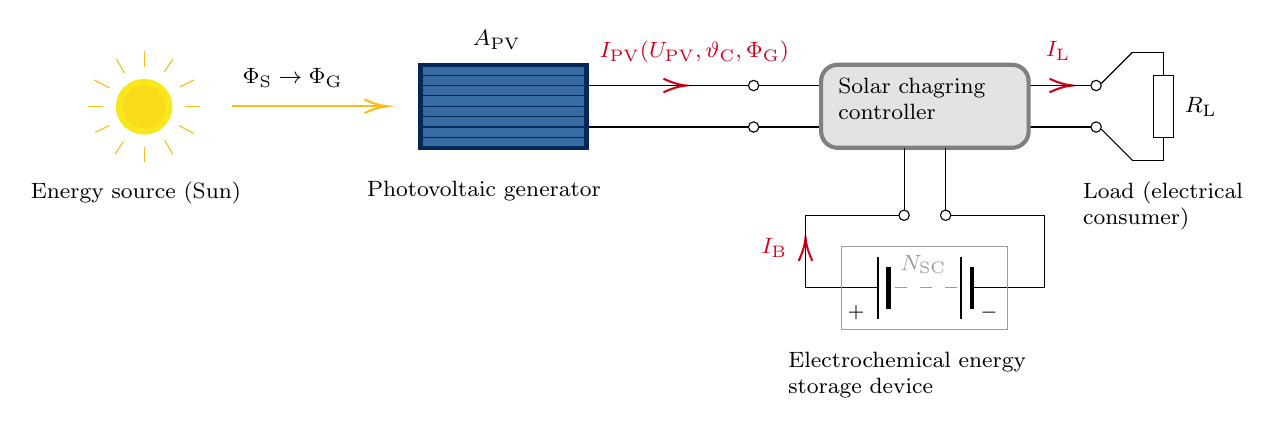
\begin{tikzpicture}[x=0.75pt,y=0.75pt,yscale=-1,xscale=1]
%uncomment if require: \path (0,411); %set diagram left start at 0, and has height of 411

%Straight Lines [id:da8136196719593345] 
\draw [color={rgb, 255:red, 208; green, 2; blue, 27 }  ,draw opacity=1 ]   (382.5,228.5) -- (382.5,215.5) ;
\draw [shift={(382.5,213.5)}, rotate = 450] [color={rgb, 255:red, 208; green, 2; blue, 27 }  ,draw opacity=1 ][line width=0.75]    (10.93,-3.29) .. controls (6.95,-1.4) and (3.31,-0.3) .. (0,0) .. controls (3.31,0.3) and (6.95,1.4) .. (10.93,3.29)   ;
%Straight Lines [id:da7467198195912443] 
\draw [color={rgb, 255:red, 208; green, 2; blue, 27 }  ,draw opacity=1 ]   (496,140) -- (509,140) ;
\draw [shift={(511,140)}, rotate = 180] [color={rgb, 255:red, 208; green, 2; blue, 27 }  ,draw opacity=1 ][line width=0.75]    (10.93,-3.29) .. controls (6.95,-1.4) and (3.31,-0.3) .. (0,0) .. controls (3.31,0.3) and (6.95,1.4) .. (10.93,3.29)   ;
%Straight Lines [id:da8214665589366665] 
\draw [color={rgb, 255:red, 208; green, 2; blue, 27 }  ,draw opacity=1 ]   (305,140) -- (323,140) ;
\draw [shift={(325,140)}, rotate = 180] [color={rgb, 255:red, 208; green, 2; blue, 27 }  ,draw opacity=1 ][line width=0.75]    (10.93,-3.29) .. controls (6.95,-1.4) and (3.31,-0.3) .. (0,0) .. controls (3.31,0.3) and (6.95,1.4) .. (10.93,3.29)   ;
%Straight Lines [id:da05884283577747018] 
\draw    (277,160) -- (355,160) ;
%Straight Lines [id:da06536461743866195] 
\draw    (277,140) -- (355,140) ;
%Shape: Ellipse [id:dp7367390116189665] 
\draw  [color={rgb, 255:red, 248; green, 231; blue, 28 }  ,draw opacity=1 ][fill={rgb, 255:red, 248; green, 220; blue, 28 }  ,fill opacity=1 ][line width=2.25]  (51.71,150.21) .. controls (51.71,143.62) and (57.15,138.27) .. (63.85,138.27) .. controls (70.55,138.27) and (75.98,143.62) .. (75.98,150.21) .. controls (75.98,156.81) and (70.55,162.15) .. (63.85,162.15) .. controls (57.15,162.15) and (51.71,156.81) .. (51.71,150.21) -- cycle ;
%Straight Lines [id:da6220717030144096] 
\draw [color={rgb, 255:red, 248; green, 189; blue, 28 }  ,draw opacity=1 ]   (63.85,123.5) -- (63.85,130.93) ;
%Straight Lines [id:da8051708851804078] 
\draw [color={rgb, 255:red, 248; green, 189; blue, 28 }  ,draw opacity=1 ]   (91,150.21) -- (83.45,150.21) ;
%Straight Lines [id:da3460695789100754] 
\draw [color={rgb, 255:red, 248; green, 189; blue, 28 }  ,draw opacity=1 ]   (63.85,176.93) -- (63.85,169.49) ;
%Straight Lines [id:da2732251675151305] 
\draw [color={rgb, 255:red, 248; green, 189; blue, 28 }  ,draw opacity=1 ]   (44.25,150.21) -- (36.7,150.21) ;
%Straight Lines [id:da4407496963374895] 
\draw [color={rgb, 255:red, 248; green, 189; blue, 28 }  ,draw opacity=1 ]   (80.59,159.29) -- (87.88,163.11) ;
%Straight Lines [id:da383911411945429] 
\draw [color={rgb, 255:red, 248; green, 189; blue, 28 }  ,draw opacity=1 ]   (39.82,137.32) -- (47.1,141.14) ;
%Straight Lines [id:da9217210977387595] 
\draw [color={rgb, 255:red, 248; green, 189; blue, 28 }  ,draw opacity=1 ]   (87.88,137.32) -- (81.02,140.66) ;
%Straight Lines [id:da03325396834222771] 
\draw [color={rgb, 255:red, 248; green, 189; blue, 28 }  ,draw opacity=1 ]   (47.1,159.29) -- (40.25,162.63) ;
%Straight Lines [id:da12285363488917289] 
\draw [color={rgb, 255:red, 248; green, 189; blue, 28 }  ,draw opacity=1 ]   (73.56,133.47) -- (77.68,127.29) ;
%Straight Lines [id:da4786379847065507] 
\draw [color={rgb, 255:red, 248; green, 189; blue, 28 }  ,draw opacity=1 ]   (49.77,173.11) -- (53.9,166.93) ;
%Straight Lines [id:da261341351601285] 
\draw [color={rgb, 255:red, 248; green, 189; blue, 28 }  ,draw opacity=1 ]   (73.8,166.45) -- (77.68,173.14) ;
%Straight Lines [id:da4643507370218185] 
\draw [color={rgb, 255:red, 248; green, 189; blue, 28 }  ,draw opacity=1 ]   (50.5,127.29) -- (54.38,133.98) ;

%Straight Lines [id:da8936580886091565] 
\draw [color={rgb, 255:red, 248; green, 189; blue, 28 }  ,draw opacity=1 ][line width=0.75]    (179,150) -- (106,150) ;
\draw [shift={(181,150)}, rotate = 180] [color={rgb, 255:red, 248; green, 189; blue, 28 }  ,draw opacity=1 ][line width=0.75]    (10.93,-3.29) .. controls (6.95,-1.4) and (3.31,-0.3) .. (0,0) .. controls (3.31,0.3) and (6.95,1.4) .. (10.93,3.29)   ;
%Shape: Circle [id:dp07158046691092301] 
\draw   (355,160) .. controls (355,158.62) and (356.12,157.5) .. (357.5,157.5) .. controls (358.88,157.5) and (360,158.62) .. (360,160) .. controls (360,161.38) and (358.88,162.5) .. (357.5,162.5) .. controls (356.12,162.5) and (355,161.38) .. (355,160) -- cycle ;
%Shape: Circle [id:dp25309308645033757] 
\draw   (355,140) .. controls (355,138.62) and (356.12,137.5) .. (357.5,137.5) .. controls (358.88,137.5) and (360,138.62) .. (360,140) .. controls (360,141.38) and (358.88,142.5) .. (357.5,142.5) .. controls (356.12,142.5) and (355,141.38) .. (355,140) -- cycle ;
%Straight Lines [id:da08781161374086754] 
\draw    (490,140) -- (520,140) ;
%Straight Lines [id:da1141924880655707] 
\draw    (490,160) -- (520,160) ;
%Shape: Circle [id:dp18646523024055295] 
\draw   (520,140) .. controls (520,138.62) and (521.12,137.5) .. (522.5,137.5) .. controls (523.88,137.5) and (525,138.62) .. (525,140) .. controls (525,141.38) and (523.88,142.5) .. (522.5,142.5) .. controls (521.12,142.5) and (520,141.38) .. (520,140) -- cycle ;
%Shape: Circle [id:dp3179313012599374] 
\draw   (520,160) .. controls (520,158.62) and (521.12,157.5) .. (522.5,157.5) .. controls (523.88,157.5) and (525,158.62) .. (525,160) .. controls (525,161.38) and (523.88,162.5) .. (522.5,162.5) .. controls (521.12,162.5) and (520,161.38) .. (520,160) -- cycle ;
%Straight Lines [id:da3754937570361223] 
\draw    (560,135) -- (550,135) ;
%Straight Lines [id:da28765380259572004] 
\draw    (560,165) -- (550,165) ;
%Straight Lines [id:da7994093769920398] 
\draw    (550,165) -- (550,135) ;
%Straight Lines [id:da49571728514760194] 
\draw    (560,165) -- (560,135) ;
%Straight Lines [id:da8708596386928309] 
\draw    (525,139) -- (540,124) ;
%Straight Lines [id:da34435901343623154] 
\draw    (360,140) -- (390,140) ;
%Straight Lines [id:da885690749449715] 
\draw    (360,160) -- (390,160) ;
%Straight Lines [id:da5154787772311555] 
\draw    (525,161) -- (540,176) ;
%Straight Lines [id:da8283908147650987] 
\draw    (540,124) -- (555,124) ;
%Straight Lines [id:da576788078319086] 
\draw    (540,176) -- (555,176) ;
%Straight Lines [id:da1720155229910998] 
\draw    (555,124) -- (555,135) ;
%Straight Lines [id:da2995787552008038] 
\draw    (555,165) -- (555,176) ;
%Rounded Rect [id:dp605862839350801] 
\draw  [color={rgb, 255:red, 128; green, 128; blue, 128 }  ,draw opacity=1 ][fill={rgb, 255:red, 227; green, 227; blue, 227 }  ,fill opacity=1 ][line width=1.5]  (390,138) .. controls (390,133.58) and (393.58,130) .. (398,130) -- (482,130) .. controls (486.42,130) and (490,133.58) .. (490,138) -- (490,162) .. controls (490,166.42) and (486.42,170) .. (482,170) -- (398,170) .. controls (393.58,170) and (390,166.42) .. (390,162) -- cycle ;
%Shape: Rectangle [id:dp22380146308476956] 
\draw  [color={rgb, 255:red, 0; green, 41; blue, 90 }  ,draw opacity=1 ][fill={rgb, 255:red, 57; green, 107; blue, 163 }  ,fill opacity=1 ][line width=1.5]  (197,130) -- (277,130) -- (277,170) -- (197,170) -- cycle ;
%Straight Lines [id:da2633344010900689] 
\draw [color={rgb, 255:red, 0; green, 41; blue, 90 }  ,draw opacity=1 ]   (197,135) -- (277,135) ;
%Straight Lines [id:da7329634137016672] 
\draw [color={rgb, 255:red, 0; green, 41; blue, 90 }  ,draw opacity=1 ]   (197,140) -- (277,140) ;
%Straight Lines [id:da3363363364783303] 
\draw [color={rgb, 255:red, 0; green, 41; blue, 90 }  ,draw opacity=1 ]   (197,150) -- (277,150) ;
%Straight Lines [id:da5631412852438793] 
\draw [color={rgb, 255:red, 0; green, 41; blue, 90 }  ,draw opacity=1 ]   (197,145) -- (277,145) ;
%Straight Lines [id:da6153878400696737] 
\draw [color={rgb, 255:red, 0; green, 41; blue, 90 }  ,draw opacity=1 ]   (197,155) -- (277,155) ;
%Straight Lines [id:da7384152042955765] 
\draw [color={rgb, 255:red, 0; green, 41; blue, 90 }  ,draw opacity=1 ]   (197,160) -- (277,160) ;
%Straight Lines [id:da4382619041484126] 
\draw [color={rgb, 255:red, 0; green, 41; blue, 90 }  ,draw opacity=1 ]   (197,165) -- (277,165) ;

%Straight Lines [id:da3400420847168515] 
\draw    (450,170) -- (450,200) ;
%Straight Lines [id:da6795701825095302] 
\draw    (430,170) -- (430,200) ;

%Shape: Circle [id:dp030153076038484272] 
\draw   (447.5,202.5) .. controls (447.5,201.12) and (448.62,200) .. (450,200) .. controls (451.38,200) and (452.5,201.12) .. (452.5,202.5) .. controls (452.5,203.88) and (451.38,205) .. (450,205) .. controls (448.62,205) and (447.5,203.88) .. (447.5,202.5) -- cycle ;
%Shape: Circle [id:dp08428574429470248] 
\draw   (427.5,202.5) .. controls (427.5,201.12) and (428.62,200) .. (430,200) .. controls (431.38,200) and (432.5,201.12) .. (432.5,202.5) .. controls (432.5,203.88) and (431.38,205) .. (430,205) .. controls (428.62,205) and (427.5,203.88) .. (427.5,202.5) -- cycle ;
%Straight Lines [id:da024547296314676226] 
\draw    (402.5,237.5) -- (382.5,237.5) ;
%Straight Lines [id:da8993285949308742] 
\draw [line width=0.75]    (417.5,222.5) -- (417.5,252.5) ;
%Straight Lines [id:da9178918649128838] 
\draw [color={rgb, 255:red, 155; green, 155; blue, 155 }  ,draw opacity=1 ] [dash pattern={on 4.5pt off 4.5pt}]  (455.5,237.5) -- (420.5,237.5) ;
%Straight Lines [id:da3598630804907186] 
\draw [line width=1.5]    (422.5,227.5) -- (422.5,247.5) ;
%Straight Lines [id:da4254329027835011] 
\draw [line width=0.75]    (457.5,222.5) -- (457.5,252.5) ;
%Straight Lines [id:da7513947415530464] 
\draw [line width=1.5]    (462.5,227.5) -- (462.5,247.5) ;
%Straight Lines [id:da24748868677387104] 
\draw    (417.5,237.5) -- (402.5,237.5) ;
%Straight Lines [id:da009805082115965202] 
\draw    (477.5,237.5) -- (462.5,237.5) ;
%Straight Lines [id:da7428727764436842] 
\draw    (497.5,237.5) -- (477.5,237.5) ;
%Shape: Rectangle [id:dp13613803613375608] 
\draw  [color={rgb, 255:red, 155; green, 155; blue, 155 }  ,draw opacity=1 ] (480,217.5) -- (480,257.5) -- (400,257.5) -- (400,217.5) -- cycle ;
%Straight Lines [id:da9313000955522079] 
\draw    (452.5,202.5) -- (497.5,202.5) ;
%Straight Lines [id:da4244913203234748] 
\draw    (382.5,202.5) -- (427.5,202.5) ;
%Straight Lines [id:da11099998272282585] 
\draw    (382.5,202.5) -- (382.5,237.5) ;
%Straight Lines [id:da2340928507704263] 
\draw    (497.5,202.5) -- (497.5,237.5) ;

% Text Node
\draw (8,185) node [anchor=north west][inner sep=0.75pt]  [font=\footnotesize] [align=left] {Energy source (Sun)};
% Text Node
\draw (170,185) node [anchor=north west][inner sep=0.75pt]  [font=\footnotesize] [align=left] {Photovoltaic generator};
% Text Node
\draw (110,130.4) node [anchor=north west][inner sep=0.75pt]  [font=\footnotesize]  {$\Phi _{\mathrm{S}}\rightarrow \Phi _{\mathrm{G}}$};
% Text Node
\draw (282,117.4) node [anchor=north west][inner sep=0.75pt]  [font=\footnotesize,color={rgb, 255:red, 208; green, 2; blue, 27 }  ,opacity=1 ]  {$I_{\mathrm{PV}}( U_{\mathrm{PV}} ,\vartheta _{\mathrm{C}} ,\Phi _{\mathrm{G}})$};
% Text Node
\draw (397.08,135) node [anchor=north west][inner sep=0.75pt]  [font=\footnotesize] [align=left] {Solar chagring\\controller};
% Text Node
\draw (515,185) node [anchor=north west][inner sep=0.75pt]  [font=\footnotesize] [align=left] {Load (electrical \\consumer)};
% Text Node
\draw (497,117.4) node [anchor=north west][inner sep=0.75pt]  [font=\footnotesize,color={rgb, 255:red, 208; green, 2; blue, 27 }  ,opacity=1 ]  {$I_{\mathrm{L}}$};
% Text Node
\draw (401.5,244.9) node [anchor=north west][inner sep=0.75pt]  [font=\scriptsize]  {$+$};
% Text Node
\draw (465.5,244.9) node [anchor=north west][inner sep=0.75pt]  [font=\scriptsize]  {$-$};
% Text Node
\draw (427,220.4) node [anchor=north west][inner sep=0.75pt]  [font=\footnotesize,color={rgb, 255:red, 155; green, 155; blue, 155 }  ,opacity=1 ]  {$N_{\mathrm{SC}}$};
% Text Node
\draw (360,212.4) node [anchor=north west][inner sep=0.75pt]  [font=\footnotesize,color={rgb, 255:red, 208; green, 2; blue, 27 }  ,opacity=1 ]  {$I_{\mathrm{B}}$};
% Text Node
\draw (373,267) node [anchor=north west][inner sep=0.75pt]  [font=\footnotesize] [align=left] {Electrochemical energy\\storage device};
% Text Node
\draw (564,144.4) node [anchor=north west][inner sep=0.75pt]  [font=\footnotesize]  {$R_{\mathrm{L}}$};
% Text Node
\draw (221,112.4) node [anchor=north west][inner sep=0.75pt]  [font=\footnotesize]  {$A_{\mathrm{PV}}$};


\end{tikzpicture}

	\caption{Basic structure of an electrical stand-alone system which is supplied with electrical energy by a photovoltaic generator. The energy is stored in an electrochemical energy storage device.}
	\label{fig:tikz/tikz_solar_energy_distribution}
\end{figure}
As illustrated in figure \ref{fig:tikz/tikz_solar_energy_distribution}, the radiation flux $\Phi_{\mathrm{G}}$ in $\left( \mathrm{W} \right)$ onto the PV generator's \emph{energy-converting area} $A_{\mathrm{PV}}$ in $\left( \mathrm{m}^2 \right)$ can be converted into electrical energy. This results in the \emph{PV generator current} $I_{\mathrm{PV}}\left( U_{\mathrm{PV}}, \vartheta_\mathrm{C}, \Phi_\mathrm{G} \right)$ in $\left( \mathrm{A} \right)$. In addition to the radiation flux $\Phi_\mathrm{G}$, this current depends on the \emph{PV generator voltage}\footnote{$I_{\mathrm{PV}}\left( U_{\mathrm{PV}} \right)$ defines the current-voltage characteristic of a PV generator.} $U_{\mathrm{PV}}$ in $\left( \mathrm{V} \right)$ and the \emph{temperature} of the PV cells -- of which the PV generator consists -- $\vartheta_{\mathrm{C}}$ in $\left( ^\circ \mathrm{C} \right)$, as this temperature plays an important role in the power output of a PV generator. For both, the PV generator and the load, the upper electrical connection (circle) represents the positive electric potential, from which the reference directions for the electrical currents directly follow. $I_\mathrm{B}$ in $\left( \mathrm{A}\right)$ is the \emph{battery current} and $I_\mathrm{L}$ in $\left( \mathrm{A}\right)$ is the \emph{load current}. \cite{Ley:2011, Bertol:2011, Mertens:2015}.

With regard to future Mars missions the authors of the articles \cite{Appelbaum:1990, Appelbaum:1992, Landis:1995} found out, that even during prolonged Martian dust storms -- when the Martian atmosphere becomes almost opaque -- a PV generator could still convert electrical energy, due to the diffuse component of sunlight. This is suppored by empirical data measured with PV generators on Earth as shown in the book \cite{Mertens:2015} and by solar resource maps for Earth's surface provided by \cite{SolargisMaps:2020, GlobalSolarAtlas:2020, Union:2020}. The authors of the article \cite[1]{Landis:1995} furthermore state: \textit{``Solar energy is likely to be an important power source for surface-bound operations on Mars.''}, which is another reason why solar energy was selected as a renewable energy source to supply the self-sufficient voice communication system.

In the following subsections the modeling of the self-sufficient energy distribution system of the voice communication system on Earth will be explained. The last subsection adapts these findings to a Martian application. % Change this if necessary

% Subsections:
\subsection{Angular relationships} \label{sec:angular_relationships}
Before the energy yield of a PV generator can be calculated, it is essential to introduce a few important angles -- of which some were already mentioned -- and define how they are counted in this thesis.

The local latitude $\varphi$ at the equator is $0^\circ$ and it is counted positive towards the north and negative towards the south with a range of $\left[-90^\circ \text{, } 90^\circ\right]$, and the local \emph{longitude} $\lambda$ in $\left(^\circ\right)$ is $0^\circ$ at the reference meridian $\lambda_0$ in $\left(^\circ\right)$ which passes through the Greenwich Observatory in the United Kingdom. $\lambda$ is counted positive east and negative west of Greenwich with a range of $\left(-180^\circ \text{, } 180^\circ\right]$ \cite{Landis:1995, Karttunen:2006, Wagner:2018}. For completens it should be mentioned that the latitude $\varphi$ and the longitude $\lambda$ -- for a given location on Earth -- can be obtained from an atlas or a \emph{global positioning system} (GPS) device.

The Sun's declination $\delta$ indicates how far the Earth's axis of rotations -- which runs through the North and South Poles -- leans towards the Sun at solar noon. Its range is $\left[-90^\circ \text{, } 90^\circ\right]$, although its maximum values for Earth are $-23,45^\circ$ and $23,45^\circ$. $\delta$ is counted negative if the North Pole leans away from the Sun and positive if it leans towards the Sun (compare to figure \ref{fig:tikz_angular_relationship}) \cite{Landis:1995, Karttunen:2006, Mertens:2015, Wagner:2018}. As per \cite{Wagner:2018}, the following approximation for $\delta$ at a given day of the year, with $N_d$ being the \emph{number of days} since January 1\textsuperscript{st} in $\left(\mathrm d \right)$,  $mon$ being the \emph{month} in $\left( 1 \right)$ and $d$ being the \emph{day} in $\left(\mathrm d \right)$, is sufficient for photovoltaic applications: 
	\begin{equation} \label{eq:delta}
	\centering
		\delta \approx 23,45^\circ \cdot \sin \left(360^\circ \cdot \frac{284\mathrm{d} + N_d}{365\mathrm{d}}\right) \text{,} 
	\end{equation}
	\begin{equation} \label{eq:delta}
	\centering
		N_d \approx 30,3\mathrm{d} \cdot \left(mon - 1\right) + d \text{.}
	\end{equation}

The altitude $\gamma_{\mathrm{S}}$ and the \emph{azimuth} $\alpha_{\mathrm{S}}$ of the Sun in $\left(^\circ \right)$, presented in the equations (\ref{eq:sin_gamma_s}) and (\ref{eq:cos_alpha_s}), describe its position in the sky over the course of the day, with $\gamma_{\mathrm{S}}$ taking on values within $\left[0^\circ \text{, } 90^\circ\right]$ and $\alpha_{\mathrm{S}}$ taking on values within $\left(-180^\circ \text{, } 180^\circ \right]$. How these angles are measured -- with the corresponding celstial hemisphere of an observer -- is shown in the figure \ref{fig:tikz_gamma_s_alpha_s}. For $\gamma_{\mathrm{S}} = 0^\circ$ the Sun is visible at the horizon and for $\gamma_{\mathrm{S}} = 90^\circ$ it is visible at its zenith. For $\alpha_{\mathrm{S}} = 0^\circ$ the Sun is visible exactly in the south. $\alpha_{\mathrm{S}}$ takes on positive values towards the west and negative values towards the east \cite{Landis:1995, Karttunen:2006, Mertens:2015, Wagner:2018}.
	\begin{equation} \label{eq:sin_gamma_s}
	\centering
		\sin \gamma_{\mathrm{S}} = \sin \varphi \, \sin \delta + \cos \varphi \, \cos \delta \, \cos h_{\mathrm{S}}
	\end{equation}
	\begin{equation} \label{eq:cos_alpha_s}
	\centering
		\cos \alpha_{\mathrm{S}} = \frac{\sin \varphi \, \cos \delta \, \cos h_{\mathrm{S}} - \cos \varphi \, \sin \delta}{\cos \gamma_{\mathrm{S}}}
	\end{equation}
\begin{figure}[h!]
	\centering
	\input{tikz/tikz_gamma_s_alpha_s}
	\caption{Angular relationship of the Sun's altitude $\gamma_{\mathrm{S}}$ and azimuth $\alpha_{\mathrm{S}}$ with the corresponding celestial hemisphere of an observer. In this figure the Sun already passed the solar noon. (Recreated from: \cite{Mertens:2015})}
	\label{fig:tikz_gamma_s_alpha_s}
\end{figure}

It must be noted that $\gamma_{\mathrm{S}}$ and $\alpha_{\mathrm{S}}$ change over the course of the day. By analyzing the equations (\ref{eq:sin_gamma_s}) and (\ref{eq:cos_alpha_s}), while taking into account that $\varphi$ does not change because the self-sufficient voice communication system is stationary for the entire mission and that in this thesis $\delta$ is modeled with a constant value throughout the day -- altough it takes on different values for each day of the year -- it must be the variable $h_{\mathrm{S}}$ in $\left(^\circ\right)$ that is responsible for these changes. It is called the \emph{solar hour angle} and its value is $0^\circ$ when the Sun reaches its greatest daily altitude $\gamma_{\mathrm{S}}$, which occurs at solar noon. This happens for either $\alpha_{\mathrm{S}} = 0^\circ$, $\alpha_{\mathrm{S}} = 180^\circ$ or for $\gamma_{\mathrm{S}} = 90^\circ$, where $\alpha_{\mathrm{S}}$ is undefined. $h_{\mathrm{S}}$ is counted negative before the solar noon and positive after the solar noon with a range of $\left(-180^\circ \text{, } 180^\circ\right]$. \cite{Landis:1995, Karttunen:2006, Mertens:2015, Wagner:2018}.  

For a given \emph{solar time}\footnote{In most cases the solar time $t_\mathrm{S}$ differs from the local time on a wrist watch. For $t_\mathrm{S} = 12\mathrm{h}$ (solar noon) the Sun is either exaclty in the south, in the north or at its zenith, whereas the Sun might not be exactly in the south, in the north or at its zenith for the \emph{local time} $t_\mathrm{local} = 12\mathrm{h}$ on a wrist watch -- no matter how accurate it is set to the local time.} $t_\mathrm{S}$ in $\left(\mathrm h \right)$, the hour angle $h_\mathrm{S}$ can be determined as shown in equation (\ref{eq:solar_hour_angle}). The factor $\frac{15^\circ}{1\mathrm{h}}$ comes about because the Earth rotates $360^\circ$ within $24\mathrm{h}$. Thus the range of the solar time $t_\mathrm{S}$ can be derived to $\left[0\mathrm{h} \text{, } 24\mathrm{h}\right)$. Further, the hour angle for the \emph{solar sunrise time} $t_\mathrm{S,r}$ in $\left(\mathrm h \right)$ and the \emph{solar sunset time} $t_\mathrm{S,s}$ in $\left(\mathrm h \right)$ can be calculated with the equations (\ref{eq:h_sunrise}) and (\ref{eq:h_sunset}) \cite{Landis:1995, Karttunen:2006, Mertens:2015, Wagner:2018}.
	\begin{equation} \label{eq:solar_hour_angle}
	\centering
		h_\mathrm{S} = \left(t_\mathrm{S} - 12\mathrm{h} \right) \cdot \frac{15^\circ}{1\mathrm{h}}
	\end{equation}
	\begin{equation} \label{eq:h_sunrise}
	\centering
		h_\mathrm{S,r} = - \arccos \left( -\tan \delta \tan \, \varphi \right) \text{,} \quad \text{for } \left|\varphi\right| < 90^\circ - \left|\delta\right|
	\end{equation}
	\begin{equation} \label{eq:h_sunset}
	\centering
		h_\mathrm{S,s} = \arccos \left( -\tan \delta \, \tan \varphi \right) \text{,} \quad \text{for } \left|\varphi\right| < 90^\circ - \left|\delta\right|
	\end{equation}

In the article \cite{Landis:1995} a few importnat cases, regarding the equations (\ref{eq:h_sunrise}) and (\ref{eq:h_sunset}), are mentioned which might be of interest when selecting a locations to install the self-sufficient voice communication system:
%\vspace{2mm}
\[ \tan \delta \, \tan \varphi \,
  \begin{cases}
    > 1       	& \text{polar night, if } \varphi < -90^\circ + \delta \text{ or } \varphi > 90^\circ + \delta \text{,} \\
    = \pm 1  		& \text{the Sun is only visible at the horizon for an instant,} \\
    < -1		& \text{polar day, if } \varphi < -90^\circ - \delta \text{ or } \varphi > 90^\circ - \delta \text{.}
  \end{cases}
\]
%\vspace{2mm}

The solar time $t_\mathrm{S}$ can finally be calculated from $t_\mathrm{UTC}$ in $\left(\mathrm h \right)$, which is the \emph{Coordinated Universal Time} (UTC), using the equation (\ref{eq:solar_time}) where $\lambda_0 = 0^\circ$ is the reference meridian for which $t_\mathrm{UTC}$ applies and $Z_{\mathrm{h}}$ in $\left(\mathrm{h}\right)$ is the \emph{equation of time} which serves as a correction factor  \cite{Karttunen:2006, Wagner:2018}.
	\begin{equation} \label{eq:solar_time}
	\centering
		t_\mathrm{S} = t_\mathrm{UTC} + Z_{\mathrm{h}} + \left(\lambda - \lambda_{\mathrm{0}}\right) \cdot \frac{1\mathrm{h}}{15\degree}
	\end{equation}
	\begin{equation} \label{eq:time_equation}
	\centering
		Z_{\mathrm{h}} \approx 0,123\mathrm{h} \cdot \cos \left(360^\circ \cdot \frac{88\mathrm{d} + N_d}{365\mathrm{d}}\right) - 0,167\mathrm{h} \cdot \sin \left(720^\circ \cdot \frac{10\mathrm{d} + N_d}{365\mathrm{d}}\right) 
	\end{equation}

\subsection{Solar irradiation on the Earth's surface} \label{sec:solar_irradiation_on_earths_surface}
Compared to equation (\ref{eq:e_sun}), determining the Sun's irradiance arriving on the surface of Earth is rather complex.\footnote{The authors of the article \cite{Babikir:2020} use the Capderou method to model the incident solar radiation on Earth. In the articles\cite{Appelbaum:1990, Appelbaum:1992} this topic is investigated with a different method for the planet Mars.} Precise calculations depend on many different factors such as the changing angular relationship between the Sun and Earth throughout the year, the composition of Earth's atmosphere -- which changes the Sun's spectrum due to absorbtion and scattering effects -- and many more \cite{Landis:1995, Mertens:2015, Wagner:2018}. 

With solar resource maps however, this problem can be circumvented. They are based on satellite and atmospheric solar irradiance models and meteorological data that were designed and collected over several years. By using these maps the compromise is made that the following calculations and estimates are performed with average irradiance values instead of exact ones. Figures \ref{fig:ghi_austria} and \ref{fig:dni_austria} provided by \cite{SolargisMaps:2020, GlobalSolarAtlas:2020} show the solar resource maps of the long term average global horizontal and direct normal irradiation, from 1994 until 2018, of Austria. The scale below the maps shows daily and annual total irradiation in $\left( \mathrm{kWh}\mathrm{m}^{-2} \right)$ \cite{MeteorologicalModeling:2020, SolarRadiationModeling:2020, SolargisData:2020}. 
\begin{figure}[h!]
	\centering
  	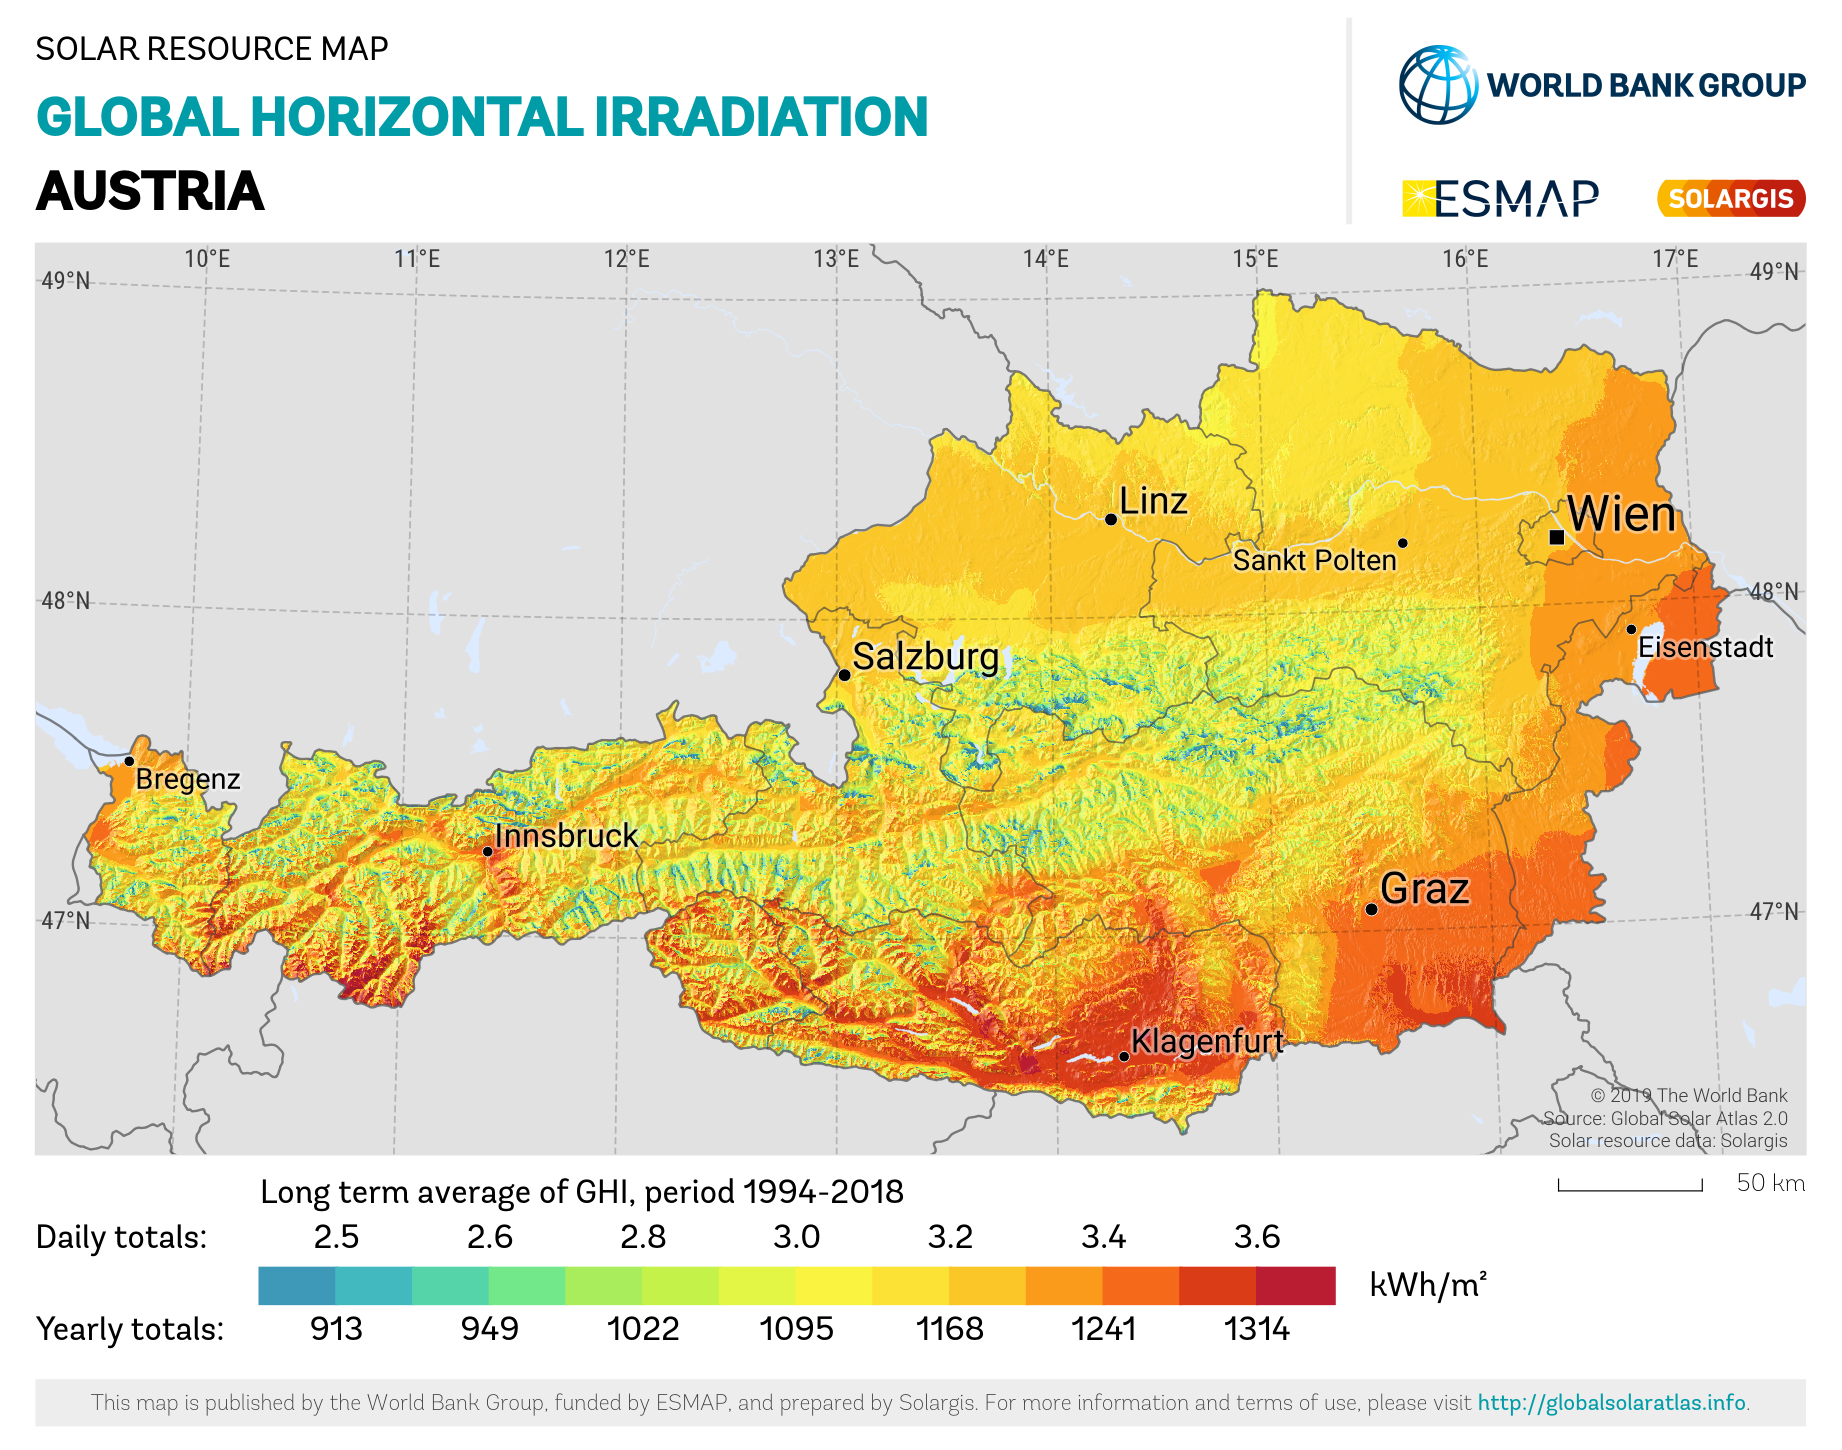
\includegraphics[width = 0.96\textwidth]{solar_maps/austria/austria_ghi}
  	\caption{Solar resource map of the long term average global horizontal irradiation of Austria. (Image credit: \cite{GlobalSolarAtlas:2020, Solargis:2021})}
	\label{fig:ghi_austria}
\end{figure}
\begin{figure}[h!]
	\centering
  	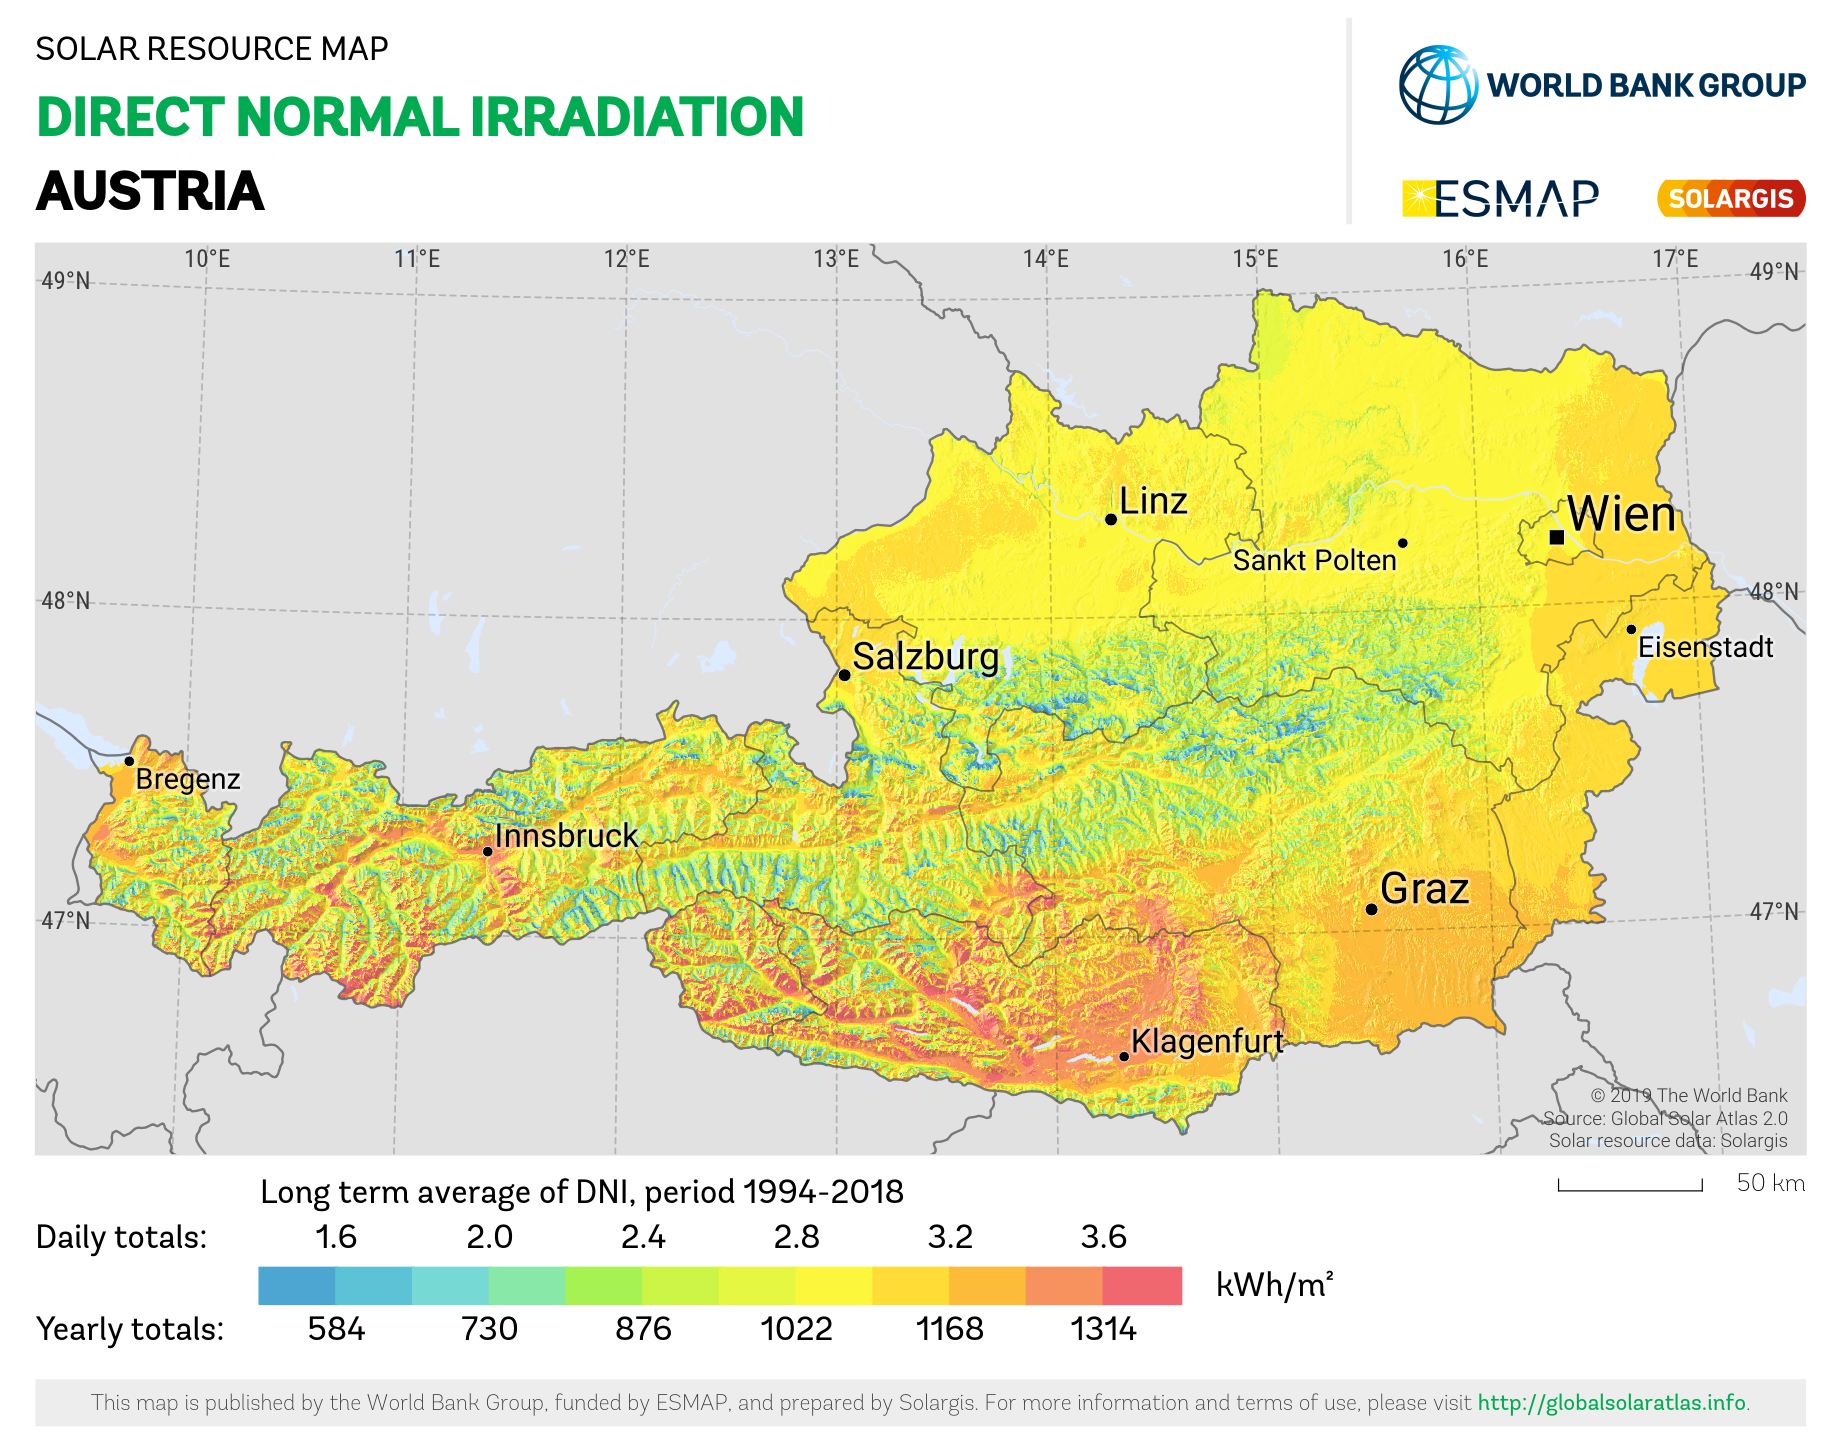
\includegraphics[width = 0.96\textwidth]{solar_maps/austria/austria_dni}
	\caption{Solar resource map of the long term average direct normal irradiation of Austria. (Image credit: \cite{GlobalSolarAtlas:2020, Solargis:2021})}
	\label{fig:dni_austria}
\end{figure}

It can be clearly seen that the values for both the global horizontal and the direct normal irradiation tend to be higher in the south and lower in the north of Austria. This can be partly explained by a greater latitude $\varphi$ which results in a lower altitude of the Sun $\gamma_{\mathrm{S}}$ during the winter months on the northern hemisphere ($\delta < 0$). Because of this, the Sun's incoming rays need to penetrate a thicker atmopshere and it is visible above the horizon for a shorter period of time over the course of the day. For locations in the south, such as the region around Klagenfurt, daily global horizontal irradiation totals of up to $3,50\mathrm{kWh}\mathrm{m}^{-2}$ and direct normal irradiation totals of up to $3,55\mathrm{kWh}\mathrm{m}^{-2}$ and higher can be expected, whereas loactions in the north, such as the region around Linz, only reach daily global horizontal irradiation totals of around $3,25\mathrm{kWh}\mathrm{m}^{-2}$ and daily direct normal irradiation totals of around $2,9\mathrm{kWh}\mathrm{m}^{-2}$. Another notable feature are valleys bordered by mountains in the south. In these valleys, and on the bounding north-facing mountain slopes, the daily global horizontal irradiation totals drop to less than $2,5\mathrm{kWh}\mathrm{m}^{-2}$ and the daily direct normal irradiation totals drop even further down to around $1,5\mathrm{kWh}\mathrm{m}^{-2}$. Examples for such valleys can be located all across the Alps and they highlight that locations with geographical features that block the direct path of the sunlight, should be discarded as installation sites for a PV generator \cite{Karttunen:2006, Mertens:2015, Wagner:2018}.

Using such maps, the \emph{global horizontal irradiance} (GHI) $E_{\mathrm{GHI}}$ in $\left( \mathrm{W}\mathrm{m}^{-2} \right)$ and the \emph{direct normal irradiance} (DNI) $E_{\mathrm{DNI}}$ in $\left( \mathrm{W}\mathrm{m}^{-2} \right)$ -- at a given location on Earth -- can be determined by dividing the values of the global horizontal and the direct normal irradiation by the time over which they were averaged. For instance by $24\mathrm{h}$ or by $365\mathrm{d} \cdot 24\mathrm{h}$ -- depending on which scale is used from the figures \ref{fig:ghi_austria} and \ref{fig:dni_austria} \cite{Mertens:2015, SolargisData:2020}.

The GHI is the sum of \emph{direct horizontal irradiance} (DHI) $E_{\mathrm{DHI}}$ in $\left( \mathrm{W}\mathrm{m}^{-2} \right)$ and the \emph{diffuse horizontal irradiance} (DIFH) $E_{\mathrm{DIFH}}$ in $\left( \mathrm{W} \mathrm{m}^{-2} \right)$ -- which is caused by the scattering of sunlight by Earth's atmosphere -- as shown in equation (\ref{eq:e_ghi}) \cite{Mertens:2015, SolarRadiationModeling:2020}.
	\begin{equation} \label{eq:e_ghi}
	\centering
		E_{\mathrm{GHI}} = E_{\mathrm{DHI}} + E_{\mathrm{DIFH}}
	\end{equation}

In comparison to the GHI -- which applies to a horizontal surface -- the DNI applies to a flat surface element perpendicular to the incoming Sun rays and it only consideres the direct irradiance \cite{Mertens:2015, SolarRadiationModeling:2020}. With simple trigonometry as shown in \cite{Mertens:2015}, the relationship between $E_{\mathrm{DNI}}$ and $E_{\mathrm{DHI}}$ can be written as:
	\begin{equation} \label{eq:e_dni}
	\centering
		E_{\mathrm{DNI}} = E_{\mathrm{DHI}} \, \frac{1}{\sin \gamma_{\mathrm{S}}} \text{.}
	\end{equation}

More precise solar resource maps for daily and monthly average global horizontal and direct normal irradiation are provided by \cite{Union:2020}.

\subsection{Photovoltaic energy yield} \label{sec:energy_yield}
As already mentioned in subsection \ref{sec:solar_irradiation_on_earths_surface} the decisive factors to determine the irradiance at a given location on the Earth's surface are the GHI and the DNI. Building on these, the three-component model as described in \cite{Landis:1995, Mertens:2015}, can be used to calculate the \emph{total irradiance} $E_{\mathrm{G}}$ in $\left( \mathrm{W}\mathrm{m}^{-2} \right)$ received by an inclined PV generator. The \emph{angle of inclination} with respect to the ground is $\beta$ in $\left( ^\circ \right)$. An example for such an inclined PV generator can be seen in the figures \ref{fig:tikz_three_component_model} and \ref{fig:tikz_angle_theta}.
\begin{figure}[h!]
	\centering
	\input{tikz/tikz_three_component_model}
	\caption{Solar radiation on an inclined photovoltaic generator with the angle $\beta$. (Recreated from: \cite{Mertens:2015})}
	\label{fig:tikz_three_component_model}
\end{figure}
Figure \ref{fig:tikz_three_component_model} illustrates that the total irradiance received by an inlcined PV generator is made up of the sum of the \emph{direct generator irradiance} (DGI) $E_{\mathrm{DGI}}$ in $\left( \mathrm{W}\mathrm{m}^{-2} \right)$, the \emph{diffuse generator irradiance} (DIFG) $E_{\mathrm{DIFG}}$ in $\left( \mathrm{W}\mathrm{m}^{-2} \right)$ and the \emph{reflected generator irradiance} (RGI) $E_{\mathrm{RGI}}$ in $\left( \mathrm{W}\mathrm{m}^{-2} \right)$. The latter is reflected with an \emph{albedo value} $\mathrm{ALB}$ in $\left( 1 \right)$ from plane earth onto the PV generator. This relationship can be written as follows \cite{Bennett:2010, Bertol:2011, Mertens:2015, Bralower:2018}:
	\begin{equation} \label{eq:e_gen}
	\centering
		E_{\mathrm{G}} = E_{\mathrm{DGI}} + E_{\mathrm{DIFG}} + E_{\mathrm{RGI}}
	\end{equation}

The first component from equation (\ref{eq:e_gen}) can be determined by considering the \emph{angle of incidence} $\theta$ of the solar rays in $\left( ^\circ \right)$ with respect to the normal of the PV generator's energy-converting area $A_{\mathrm{PV}}$, as presented in equation (\ref{eq:e_dgi}). Figure \ref{fig:tikz_angle_theta} provides an illustration of the angle $\theta$ for which the cosine can be obtained from equation (\ref{eq:cos_theta}).
	\begin{equation} \label{eq:e_dgi}
	\centering
		E_{\mathrm{DGI}} = E_{\mathrm{DNI}} \, \cos \theta
	\end{equation}
	\begin{equation} \label{eq:cos_theta}
	\centering
		\begin{aligned}
		\cos \theta &= \sin \delta \, \sin \varphi \, \cos \beta - \sin \delta \, \cos \varphi \, \sin \beta \, \cos \alpha_{\mathrm{S}}(t_\mathrm{S} = 12\mathrm{h}) \\
		&+ \cos \delta \, \cos \varphi \, \cos \beta \, \cos h_{\mathrm{S}} + \cos \delta \, \sin \varphi \, \sin \beta \, \cos \alpha_{\mathrm{S}} \, \cos h_{\mathrm{S}} \\ &+ \cos \delta \, \sin \beta \, \cos h_{\mathrm{S}} \, \sin \alpha_{\mathrm{S}}(t_\mathrm{S} = 12\mathrm{h})
		\end{aligned}
	\end{equation}
\begin{figure}[h!]
	\centering
	\input{tikz/tikz_angle_theta}
	\caption{Illustration of the incidence angle $\theta$ of the solar rays with respect to the normal to $A_\mathrm{PV}$. (Recreated from: \cite{Landis:1995})}
	\label{fig:tikz_angle_theta}
\end{figure}
The angle of incidence $\theta$ has a range of $\left[0^\circ \text{, } 90^\circ\right]$ and $\alpha_\mathrm{S}(t_\mathrm{S} = 12\mathrm{h})$ represents the orientation of the normal to $A_\mathrm{PV}$. For completenes it must be mentioned that equation (\ref{eq:sin_gamma_s}) can be derived from equation (\ref{eq:cos_theta}) with $\beta = 0^\circ$, and that in the case $\gamma_{\mathrm{S}} + \beta = 90^\circ$, the Sun's rays are perpendicular to the PV generator's energy-converting area $A_{\mathrm{PV}}$ which results in $E_{\mathrm{DGI}} = E_{\mathrm{DNI}}$ \cite{Landis:1995, Bertol:2011, Mertens:2015, Wagner:2018}.

To determine the second component from equation (\ref{eq:e_gen}) the sky is assumed to be isotropic. This means that the DIFH is evenly distributed in the entire celestial hemisphere above the PV generator. The more the PV generator is inclined the smaller the proportion of DIFG in equation (\ref{eq:e_difg}) becomes (compare to figure \ref{fig:tikz_three_component_model}) \cite{Landis:1995, Mertens:2015}. 
	\begin{equation} \label{eq:e_difg}
	\centering
		E_{\mathrm{DIFG}} = E_{\mathrm{DIFH}} \, \frac{1 + \cos \beta }{2}
	\end{equation} 
In the book \cite{Mertens:2015} it is expressly pointed out that the isotropic approach used in equation (\ref{eq:e_difg}) is only a rough approximation. This is because the sky is brighter towards the Sun than towards the horizon.\footnote{More precise equations would be difficult to derive, which would go beyond the scope of this thesis.} 

When examining the last component from equation (\ref{eq:e_gen}) it has to be taken into account that different surfaces -- on which a PV generator is placed -- reflect solar rays differently. In equation (\ref{eq:e_rgi}) this is accomplished with the factor $\mathrm{ALB}$ -- also known as the reflectivity. Similar to equation (\ref{eq:e_difg}) an isotropic approach is used \cite{Landis:1995, Dobos:2011, Mertens:2015, Bralower:2018}. 
	\begin{equation} \label{eq:e_rgi}
	\centering
		E_{\mathrm{RGI}} = E_{\mathrm{GHI}} \, \frac{1 - \cos \beta }{2} \cdot \mathrm{ALB}
	\end{equation}
Approximate albedo values for various surfaces are listed in table \ref{tab:table_albedo}. The larger the value the more solar rays are reflected. A blackbody for example has an albedo value of 0 while an absolute white surface has an albedo value of 1. The Earth has an average albedo of 0,31 \cite{Bennett:2010, Dobos:2011, Bralower:2018}.
\begin{table}[h!]
	\centering
	\input{tables/table_albedo}
	\caption{Albedo values (refelctivity) for different surfaces \cite{Dobos:2011, Bertol:2011, Mertens:2015, Bralower:2018}.}
	\label{tab:table_albedo}
\end{table}

If the three derived components $E_{\mathrm{DGI}}$, $E_{\mathrm{DIFG}}$ and $E_{\mathrm{RGI}}$ are now inserted into equation (\ref{eq:e_gen}) while considering the equations (\ref{eq:e_ghi}) and (\ref{eq:e_dni}), the total irradiance $E_{\mathrm{G}}$ received by an inclined PV generator, depending on $E_{\mathrm{GHI}}$, $E_{\mathrm{DNI}}$, $\gamma_{\mathrm{S}}$, $\beta$ and $\mathrm{ALB}$, can be obtained:
	\begin{equation} \label{eq:e_gen_ghi_dni}
	\centering
		\begin{split}
		E_{\mathrm{G}} = E_{\mathrm{DNI}} \, \cos \theta + \left(E_{\mathrm{GHI}} - E_{\mathrm{DNI}} \, \sin \gamma_{\mathrm{S}}\right) \frac{1 + \cos \beta }{2} \\ 
		+ E_{\mathrm{GHI}} \, \frac{1 - \cos \beta }{2} \cdot \mathrm{ALB} \text{.}
		\end{split}
	\end{equation}
Regarding this equation it must be noted that the angles $\gamma_{\mathrm{S}}$ and $\theta$ are time dependent and therefore $E_{\mathrm{G}}$ as well. $E_{\mathrm{GHI}}$ and $E_{\mathrm{DNI}}$ on the other hand are average values -- if taken from solar resource maps -- and can therefore be treated as constants. The angle of inclination $\beta$ as well as the albedo value $\mathrm{ALB}$ are also treated as constants. Once the PV generator is installed its inclination angle $\beta$ will not change for the entire duration of the mission. This has the consequence that the PV generator's inclined energy-converting area $A_{\mathrm{PV}}$ is only perpendicular for one pair of $\gamma_{\mathrm{S}}$ and $\alpha_{\mathrm{S}}$ at a given time of the day. Even though $\mathrm{ALB}$ is treated as a constant, there are situations in which the albedo value of a surface can change over the course of a few hours. For instance, if the PV generator is installed on a freshly snowed uncultivated field and the snow melts away. In this case $\mathrm{ALB}$ would change from 0,80 to 0,26. Such situations must be considered while simulating the PV generator's daily energy yield. This can be accomplished by considering the lowest possible albedo value for a given region \cite{Appelbaum:1992, Landis:1995, Mertens:2015}.

As described by \cite{Mertens:2015, Wagner:2018}, the radiation flux $\Phi_{\mathrm{G}}$ onto the PV generator's energy-converting area $A_{\mathrm{PV}}$ -- to be more precise the sum of the energy-converting area of the PV cells -- can be calculated as follows:
	\begin{equation} \label{eq:radiation_flux}
	\centering
		\Phi_{\mathrm{G}} = A_{\mathrm{PV}} \, E_{\mathrm{G}}\text{.} 
	\end{equation}

How to determine the optimal angle of inclination $\beta$ for a PV generator will be discussed in the next subsection.

\subsection{Photovoltaic generator alignment} \label{sec:photovoltaic_generator_alignment}
Simply put, the alignment of a stationary PV generator -- which does not actively track the Sun throughout the day, but is installed with a fixed orientation of the normal to $A_{\mathrm{PV}}$, with respect to the cardinal directions, and a constant inclination angle $\beta$ -- depends on two basic factors.

The first factor regards the Sun's direct irradiance, which reaches its greatest daily value for clear skies at solar noon ($t_{\mathrm{S}} = 12\mathrm{h}$). This is the point in time, in which $\gamma_{\mathrm{S}}$ reaches its greatest daily value, and thus the Sun's rays have the shortest path through Earth's atmosphere to the surface. The path becomes longer, the smaller $\gamma_{\mathrm{S}}$ becomes -- regardless of whether it is before or after solar noon.\footnote{Regarding the optimal inclination angle of a PV generator for clear skies, the authors of \cite[7]{Landis:1995} write: \begin{displayquote}\textit{``For clear days, the solar irradiance is symmetrical around noon and is maximum at true solar noon, $\omega = 0$.''}\end{displayquote} The angle $\omega$ represents the solar hour angle $h_{\mathrm{S}}$.} Using the \emph{air mass} (AM) value $x$, this can be expressed as follows:
	\begin{equation} \label{eq:air_mass}
	\centering
		x = \frac{1}{\sin \gamma_{\mathrm{S}}} \text{.}
	\end{equation}
For example, for $\gamma_{\mathrm{S}} = 90^\circ$  the Sun is at its zenith. This results in $x = 1$ and therefore its rays have the shortest possible path through Earth's atmosphere to the surface. Since the spectrum of the Sun on the Earth's surface changes, depending on the length of the path of the Sun's rays, this spectrum is called AM 1. The AM 0 specturm would be outside the Earth's atmosphere which corresponds to the previously mentioned solar constant $E_{\mathrm{S}}$.  \cite{Landis:1995, Bertol:2011, Mertens:2015, Wagner:2018}. 

Besides this, the second factor regards the fact that the self-sufficent voice communication system will be in use for the entire duration of a mission. Therefore it requires electrical energy throughout the day.

Based on these findings it can be said that a stationary PV generator must be aligned in a way, so that its energy-converting area $A_{\mathrm{PV}}$ is perpendicular to the Sun's rays when it reaches its greatest daily irradiance value. This occurs when the Sun's rays have the shortest path through Earth's atmosphere. As a result, the normal to $A_{\mathrm{PV}}$ must be aligned with the incoming rays for this specific point in time, hence for $t_{\mathrm{S}} = 12\mathrm{h}$. In this case, the daily electrical energy yield of a stationary PV generator can be maximized \cite{Landis:1995, Mertens:2015, Wagner:2018}.

As mentioned in subsection \ref{sec:energy_yield}, the Sun's rays are perpendicular to the energy-converting area $A_{\mathrm{PV}}$ for $\beta = 90^\circ - \gamma_{\mathrm{S}}$. After applying this to equation (\ref{eq:sin_gamma_s}) and simplifying it with trigonometric functions, the PV generator's angle of inclinations $\beta$ at a latitude $\varphi$, with Earth's axis of rotation inclined towards the Sun with the angle $\delta$, can be derived as shown in equation (\ref{eq:beta_with_delta_and_phi}) \cite{Landis:1995, Mertens:2015, Wagner:2018}.
	\begin{equation} \label{eq:beta_with_delta_and_phi}
	\centering
		\beta = \left|\varphi - \delta\right|
	\end{equation}
The \MATLAB simulation in the appendix \ref{sec:matlab_code} showed that using the absolute value of $\beta$, it can be obtained for every installation site on Earth and for every season of the year. This is also shown by the authors of \cite{Karafil:2016}.\footnote{Nevertheless, the result of $\tan \delta \, \tan \varphi$ must be taken into account.} %However, for the equation (\ref{eq:cos_theta}) the absolute value should not be used. % CHANGE

Determining how the normal to $A_{\mathrm{PV}}$ must be oriented with respect to the cardinal directions can be accomplished by solving the equations (\ref{eq:sin_gamma_s}) and (\ref{eq:cos_alpha_s}) for $t_{\mathrm{S}} = 12\mathrm{h}$. With the help of trigonometric functions this results in:
	\begin{equation} \label{eq:gamma_s_align}
	\centering
		\gamma_{\mathrm{S}} = 90^\circ - \varphi + \delta \text{,} \quad \text{for } t_{\mathrm{S}} = 12\mathrm{h}
	\end{equation}
	\begin{equation} \label{eq:alpha_s_align}
	\centering
		\alpha_{\mathrm{S}} = \arccos \left(\frac{\sin \left(\varphi - \delta\right)}{\cos \gamma_{\mathrm{S}}}\right) \text{,} \quad \text{for } t_{\mathrm{S}} = 12\mathrm{h} \text{.}
	\end{equation}
For $\alpha_{\mathrm{S}} = 0^\circ$ the Sun is visible in the south and therefore a PV generator must be oriented in a way so that the normal to $A_{\mathrm{PV}}$ points towards the south, and for $\alpha_{\mathrm{S}} = 180^\circ$ the Sun is visible in the north and therefore the normal to $A_{\mathrm{PV}}$ must point towards the north. When the Sun is at its zenith $\alpha_{\mathrm{S}}$ cannot be solved because $\gamma_{\mathrm{S}} = 90^\circ$. In this case $\varphi = \delta$, from which $\beta = 0^\circ$ follows, and therefore the normal to $A_{\mathrm{PV}}$ must point to the Sun's zenith.

A more practical approach to this can be achieved by comparing the latitude of a PV generator's installation site to the latitude $\varphi_{\mathrm{Z}}$ in $\left(^\circ\right)$, where the Sun is at its zenith for $t_{\mathrm{S}} = 12\mathrm{h}$, using a GPS device. Figure \ref{fig:crucial_latitudes} compares the three different cases of the Sun's location in the sky, depending on the installation site of a PV generator, in which $\varphi_{\mathrm{S}}$ in $\left(^\circ\right)$ is an installation site to the south and $\varphi_{\mathrm{N}}$ in $\left(^\circ\right)$ to the north of $\varphi_{\mathrm{Z}}$.

\begin{figure}[h!]
	\centering
		\begin{subfigure}[b]{0.3\linewidth}
			\input{tikz/tikz_northern_hemisphere}
			\caption{Northern latitude.}
		\end{subfigure}
		\begin{subfigure}[b]{0.3\linewidth}
			\input{tikz/tikz_phi_z}
			\caption{Sun is at its zenith.}
		\end{subfigure}
		\begin{subfigure}[b]{0.3\linewidth}
			\input{tikz/tikz_southern_hemisphere}
			\caption{Southern latitude.}
		\end{subfigure}
	\caption{Illustration of the latitude $\varphi_{\mathrm{Z}}$ on Earth at which the Sun is at its zenith for $t_{\mathrm{S}} = 12\mathrm{h}$. By comparing the latitude of the installation site of a photovoltaic generator it can be determined how it must be aligned, so that the electrical energy yield can be maximized.}
	\label{fig:crucial_latitudes}
\end{figure}

Inserting $\gamma_{\mathrm{S}} = 90^\circ$ and $t_{\mathrm{S}} = 12\mathrm{h}$ into equation (\ref{eq:sin_gamma_s}), the latitude $\varphi_{\mathrm{Z}}$ can be determined -- after applying trigonometric functions -- to:
	\begin{equation} \label{eq:phi_z}
	\centering
		\varphi_{\mathrm{Z}} = \delta \text{.}
	\end{equation}
If a PV generator is installed at a latitude south of $\varphi_{\mathrm{Z}}$, the normal to $A_{\mathrm{PV}}$ must point towards the north, and if it is installed north of $\varphi_{\mathrm{Z}}$, the normal to $A_{\mathrm{PV}}$ must point towards the south. In case the PV generator is installed at the latitude $\varphi_{\mathrm{Z}}$, then $\beta = \varphi_{\mathrm{Z}} - \delta = 0^\circ$ applies, which means that the normal to $A_{\mathrm{PV}}$ points to the Sun's zenith. The normal to $A_{\mathrm{PV}}$ can be aligned using a simple compass.

\subsection{Modeling the solar energy curve} \label{sec:solar_energy_curve}
To further estimate the electrical energy yield of a PV generator which is inclined with the angle $\beta$, the Sun's radiation flux $\Phi_{\mathrm{G}}$ onto its energy-converting area $A_{\mathrm{PV}}$ must be modeled over the course of one day. Since the Sun's irradiance is symmetrical for $t_0 = 12\mathrm{h}$ and the PV generator is assumed to be aligned so that $A_{\mathrm{PV}}$ is perpendicular to the Sun's rays for $t_0 = 12\mathrm{h}$, the Sun's radiation flux $\Phi_{\mathrm{G}}$ as a Gaussian function of the solar time $t_{\mathrm{S}}$ can be approximated as shown in the figure \ref{fig:tikz_energy_gauss}.
\begin{figure}[h!]
	\centering
	\input{tikz/tikz_energy_gauss}
	\caption{Model of the Sun's radiation flux $\Phi_{\mathrm{G}}$ onto the energy-converting area of a photovoltaic generator as a Gaussain function of the solar time $t_{\mathrm{S}}$. It is assumed that the Sun's irradiance is symmetrical around solar noon, and that the photovoltaic generator is aligned so that its energy-converting area is perpendicular to the Sun's rays at solar noon.}
	\label{fig:tikz_energy_gauss}
\end{figure}
The corresponding Gaussian function can be obtained from equation (\ref{eq:phi_gen_gauss}):
	\begin{equation} \label{eq:phi_gen_gauss}
	\centering
		\begin{gathered}
		\Phi_{\mathrm{G}}\left(t_{\mathrm{S}}\right) = \Phi_{\mathrm{max}} \, \exp\left(-\frac{(t_{\mathrm{S}} - t_0)^2}{2 \tau_\mathrm{S}^2}\right) \text{, } 
		\\
		\tau_\mathrm{S} = \frac{t_0 - t_{\mathrm{S,r}}}{3} = \frac{t_{\mathrm{S,s}} - t_0}{3} \text{.}
		\end{gathered}
	\end{equation}
The area this curve encloses with the solar time axis $t_{\mathrm{S}}$, from solar sunrise $t_{\mathrm{S,r}}$ to solar sunset $t_{\mathrm{S,s}}$, is equal to 99,7\% of the \emph{daily solar energy} $W_{\mathrm{G}}$ in $\left(\mathrm{Wh}\right)$ which occurs on the energy-converting area $A_{\mathrm{PV}}$ \cite{Landis:1995, Prechtl:2006, Prechtl:2008, Glover:2010, Schrufer:2014, AlNahhal:2019}:\footnote{$t_{\mathrm{S,r}}$ and $t_{\mathrm{S,s}}$ were selected this way for simplicity.}
	\begin{equation} \label{eq:w_gen_gauss}
	\centering
		W_\mathrm{G} = \frac{1}{0,997} \int\limits_{t_{\mathrm{S,r}}}^{t_{\mathrm{S,s}}} \Phi_{\mathrm{max}} \, \exp\left(-\frac{(t_{\mathrm{S}} - t_0)^2}{2 \tau_\mathrm{S}^2}\right) \,\mathrm{d}t_\mathrm{S} = \frac{\Phi_{\mathrm{max}} \, \tau_\mathrm{S} \sqrt{2\pi}}{0,997} \text{.}
	\end{equation}

A similar approach is used in \cite{Guo:2017, Nguyen:2020} and in \cite{Balafas:2010, Mertens:2015, Koudouris:2017} it can be seen that the Sun's total irradiance $E_{\mathrm{G}}$ throughout the day, from which $\Phi_{\mathrm{G}}$ derives, behaves similar to a Gaussian curve.\footnote{How to solve the integral in equation \ref{eq:w_gen_gauss} from $-\infty$ to $\infty$ can be found in the appendix \ref{sec:gauss_general}.}

The greates daily radiation flux $\Phi_{\mathrm{max}}$ in $\left(\mathrm W\right)$ onto $A_{\mathrm{PV}}$ can be calculated using the equations (\ref{eq:e_gen_ghi_dni}) and (\ref{eq:radiation_flux}) by deriving the following relationship:
	\begin{equation} \label{eq:w_gen}
	\centering
		W_\mathrm{G} = \int\limits_{t_{\mathrm{S,r}}}^{t_{\mathrm{S,s}}} \Phi_{\mathrm{G}}\,\mathrm{d}t_\mathrm{S} = A_{\mathrm{PV}} \int\limits_{t_{\mathrm{S,r}}}^{t_{\mathrm{S,s}}} E_{\mathrm{G}}\,\mathrm{d}t_\mathrm{S} \text{.}
	\end{equation}
Considering that $A_{\mathrm{PV}}$ is a constant factor and taking into account the findings from the subsection \ref{sec:energy_yield}, the integrals from equation (\ref{eq:w_gen}) can be partly solved as follows:
	\begin{equation} \label{eq:int_e_gen}
	\centering
		\begin{split}
		\int\limits_{t_{\mathrm{S,r}}}^{t_{\mathrm{S,s}}} E_{\mathrm{G}}\,\mathrm{d}t_\mathrm{S} = E_{\mathrm{GHI}} \left( \frac{1 + \cos \beta}{2} + \frac{1 - \cos \beta}{2} \cdot \mathrm{ALB} \right) \cdot \left(t_{\mathrm{S,s}} - t_{\mathrm{S,r}}\right) \\ 
		- E_{\mathrm{DNI}} \ \frac{1 + \cos \beta}{2} \underbrace{\int\limits_{t_{\mathrm{S,r}}}^{t_{\mathrm{S,s}}} \sin \gamma_{\mathrm{S}}\,\mathrm{d}t_\mathrm{S}}_\text{\textbf{\RN{1}}} + E_{\mathrm{DNI}} \underbrace{\int\limits_{t_{\mathrm{S,r}}}^{t_{\mathrm{S,s}}} \cos \theta \,\mathrm{d}t_\mathrm{S}}_\text{\textbf{\RN{2}}} \text{.}
		\end{split}
	\end{equation}
Using the equations (\ref{eq:sin_gamma_s}) and (\ref{eq:solar_hour_angle}), integral \text{\textbf{\RN{1}}} can be solved to:
	\begin{equation} \label{eq:int_rn_1}
	\centering
		\begin{aligned}
		\text{\textbf{\RN{1}}:} \ &\int\limits_{t_{\mathrm{S,r}}}^{t_{\mathrm{S,s}}} \sin \gamma_{\mathrm{S}}\,\mathrm{d}t_\mathrm{S} = 
		\sin \varphi \, \sin \delta \left(t_{\mathrm{S,s}} - t_{\mathrm{S,r}} \right) \\
		&+ c_{\varphi,\delta} \left(\sin \left(\left(t_{\mathrm{S,s}} - 12\mathrm{h} \right) \cdot \frac{15^\circ}{1\mathrm{h}} \right) - \sin \left(\left( t_{\mathrm{S,r}} - 12\mathrm{h} \right) \cdot \frac{15^\circ}{1\mathrm{h}} \right)\right) \text{,}
		\end{aligned}
	\end{equation}
with $c_{\varphi,\delta}$ being:
	\begin{equation} \label{eq:const_varphi_delta}
	\centering
		c_{\varphi,\delta} = \cos \varphi \, \cos \delta \cdot \frac{1\mathrm{h}}{15^\circ} \text{.}
	\end{equation}
Integral \text{\textbf{\RN{2}}} on the other hand cannot be solved analytically as easy. This is why a sum instead of an integral is used in the \MATLAB simulation (see appendix \ref{sec:matlab_code}) to calculate $W_{\mathrm{G}}$:
	\begin{equation} \label{eq:sum_energy}
	\centering
		W_\mathrm{G} = A_{\mathrm{PV}} \displaystyle\sum_{t_{\mathrm{S}} = t_{\mathrm{S,r}}}^{t_{\mathrm{S,s}}} E_{\mathrm{G}} \, \Delta t_{\mathrm{S}} \text{.}
	\end{equation}
Using trigonometric functions, $E_{\mathrm{G}}$ can be simplyfied as shown in the equation (\ref{eq:sum_e_gen}). Depending on the desired accuracy $\Delta t_{\mathrm{S}}$ in $\left( \mathrm{h} \right)$ can be smaller or greater. The smaller it is the more accurate $W_{\mathrm{G}}$ can be modeled.\footnote{$\Delta t_{\mathrm{S}}$ is one discrete time step of the solar time. It can be caluculated from the length $len$ of the Matlab vector that goes from $t_{\mathrm{S,r}}$ to $t_{\mathrm{S,s}}$: $\Delta t_{\mathrm{S}} = \frac{1}{len}$.}
	\begin{equation} \label{eq:sum_e_gen}
	\centering
		\begin{aligned}
		\displaystyle\sum_{t_{\mathrm{S}} = t_{\mathrm{S,r}}}^{t_{\mathrm{S,s}}} E_{\mathrm{G}} \, \Delta t_{\mathrm{S}} &= \displaystyle\sum_{t_{\mathrm{S}} = t_{\mathrm{S,r}}}^{t_{\mathrm{S,s}}} \left(E_{\mathrm{GHI}} - E_{\mathrm{DNI}} \, \sin \gamma_{\mathrm{S}} \right) \cos^2 \frac{\beta}{2} \, \Delta t_{\mathrm{S}} \\
		&+ \displaystyle\sum_{t_{\mathrm{S}} = t_{\mathrm{S,r}}}^{t_{\mathrm{S,s}}} \left(E_{\mathrm{DNI}} \, \cos \theta + E_{\mathrm{GHI}} \, \sin^2 \frac{\beta}{2} \cdot \mathrm{ALB} \right)\Delta t_{\mathrm{S}}
		\end{aligned}
	\end{equation}
By inserting the caluclated $W_{\mathrm{G}}$ from equation (\ref{eq:sum_energy}) into equation (\ref{eq:w_gen_gauss}) and transforming it, the greates daily radiation flux $\Phi_{\mathrm{max}}$ onto $A_{\mathrm{PV}}$, which in this model occurs for $t_0 = 12\mathrm{h}$, can be obtained \cite{Appelbaum:1992, Landis:1995, Prechtl:2006, Prechtl:2008}:
	\begin{equation} \label{eq:phi_max_sum}
	\centering
		\Phi_{\mathrm{max}} = \frac{0,997 \cdot A_{\mathrm{PV}}}{\tau_\mathrm{S} \sqrt{2\pi}} \displaystyle\sum_{t_{\mathrm{S}} = t_{\mathrm{S,r}}}^{t_{\mathrm{S,s}}} E_{\mathrm{G}} \, \Delta t_{\mathrm{S}} \text{.}
	\end{equation}

\subsection{Photovoltaic generators} \label{sec:photovoltaic_generators}
The aim of this subsection is to model the \emph{electrical power output} $P_{\mathrm{PV}}$ in $\left( \mathrm W \right)$ of a PV generator based on the previous findings. Since most commercial PV generators consist of PV cells connected in series, only these are going to be covered. Figure \ref{fig:tikz_PVG_circuit_diagram} shows the \emph{electrical equivalent circuit} (EEC) of such a PV generator with a given \emph{number of PV cells} $N_{\mathrm{C}}$ in $\left( 1 \right)$.
\begin{figure}[h!]
	\centering
	\input{tikz/tikz_PVG_circuit_diagram}
	\caption{Electrical equivalent circuit of a photovoltaic generator. It consists of $N_{\mathrm{C}}$ photovoltaic cells connected in series. (Recreated from: \cite{Mertens:2015})}
	\label{fig:tikz_PVG_circuit_diagram}
\end{figure}
As illustrated, $I_{\mathrm{PV}}$ is equal for all PV cells and $U_{\mathrm{PV}}$ is the sum of the \emph{PV cell voltages} $U_{\mathrm{C}}$ in $\left( \mathrm{V} \right)$. It is assumed that all PV cells have the same voltage $U_{\mathrm{C}}$ and therefore $U_{\mathrm{PV}}$ can be written as presented in the equation (\ref{eq:u_pvg_sum_of_pvc}). For the sake of simplicity it is furthermore assumed that the PV generator is installed in a way so that no shadowing occurs during the course of the mission \cite{Prechtl:2006, Mertens:2015}.
	\begin{equation} \label{eq:u_pvg_sum_of_pvc}
	\centering
		U_{\mathrm{PV}} = N_{\mathrm{C}} \, U_{\mathrm{C}}
	\end{equation}

In the next step the PV cells shown in figure \ref{fig:tikz_PVG_circuit_diagram} must be modeled. For this, the simplified standard model\footnote{This model can be derived from the PV cell standard model for $R_{\mathrm{P}} \to \infty$ and $R_{\mathrm{S}} = 0\Omega$.} is used as there are explicit solutions for $U_{\mathrm{C}}$ and $I_{\mathrm{PV}}$. It represents an ideal PV cell without internal losses. An illustration of this model is provided in figure \ref{fig:tikz_PVC_simplified} \cite{Mertens:2015, Wagner:2018}.
\begin{figure}[h!]
	\centering
	\input{tikz/tikz_PVC_simplified}
	\caption{Simplified standard model of a photovoltaic cell. (Recreated from: \cite{Mertens:2015, Wagner:2018})}
	\label{fig:tikz_PVC_simplified}
\end{figure}

After applying Kirchoff's first and second law to the simplified standard model, considering the equation (\ref{eq:u_pvg_sum_of_pvc}) and taking into account that the PV generator's current-voltage characteristic depends on the PV cell temperature $\vartheta_{\mathrm{C}}$ and the radiation flux $\Phi_{\mathrm{G}}$, it can be modeled with the equations (\ref{eq:i_of_u}) and (\ref{eq:u_of_i}).\footnote{Equation (\ref{eq:u_of_i}) can be derived from equations (\ref{eq:i_of_u}).}
	\begin{equation} \label{eq:i_of_u}
	\centering
		I_{\mathrm{PV}}(U_{\mathrm{PV}}, \vartheta_{\mathrm{C}}, \Phi_{\mathrm{G}}) = I_{\mathrm{Ph}} - \underbrace{I_{\mathrm{S}} \left( \exp \left(\frac{U_{\mathrm{PV}}}{m \, N_{\mathrm{C}} \, U_{\mathrm{T}} } \right) - 1  \right)}_{I_{\mathrm{D}}}
	\end{equation}
	\begin{equation} \label{eq:u_of_i}
	\centering
		U_{\mathrm{PV}}(I_{\mathrm{PV}}, \vartheta_{\mathrm{C}}, \Phi_{\mathrm{G}}) = m \, N_{\mathrm{C}} \, U_{\mathrm{T}} \, \ln \left( \frac{I_{\mathrm{Ph}} - I_{\mathrm{PV}} + I_{\mathrm{S}}}{I_{\mathrm{S}}} \right)
	\end{equation}
The diode's \emph{thermal voltage} $U_{\mathrm{T}} = U_{\mathrm{T}}(\vartheta_{\mathrm{C}})$ in $\left( \mathrm{V} \right)$, with $k_\mathrm{B} = 1,380649 \cdot 10^{-23} \mathrm{WsK^{-1}}$ being the \emph{Bolzmann constant} and $e = 1,602176634\cdot10^{-19} \mathrm{As}$ being the \emph{elementary charge}, can be obtained from the equation (\ref{eq:u_temp}).
	\begin{equation} \label{eq:u_temp}
	\centering
		U_{\mathrm{T}}(\vartheta_{\mathrm{C}}) = \frac{ k_\mathrm{B} \left( \vartheta_{\mathrm{C}} + 273,15^\circ \mathrm{C} \right) }{e} \cdot \frac{\mathrm{1K}}{1^\circ \mathrm{C}}
	\end{equation}
$m$ in $\left( 1 \right)$ is the \emph{ideality factor} with the condition $\{m \in \mathbb{R}^+ \mid 2 \geq m \geq 1 \}$. It is an empirical value that is used to model the PV cells more precisely.\footnote{For $m = 1$, $I_\mathrm{D}$ is Shockley's equation.} The quantities $I_{\mathrm{S}} = I_{\mathrm{S}}(\vartheta_{\mathrm{C}})$ in $\left( \mathrm{A} \right)$ and $I_{\mathrm{Ph}} = I_{\mathrm{Ph}}(\vartheta_{\mathrm{C}}, \Phi_{\mathrm{G}})$ in $\left( \mathrm{A} \right)$ are the diode's \emph{reverse saturation current} and the PV cell's \emph{photocurrent} \cite{Prechtl:2006, Mertens:2015, Tietze:2016, Wagner:2018, Elert:2020}. 

Based on the equation (\ref{eq:i_of_u}), the modeled current-voltage characteristic can be visualized as shown in the figure \ref{fig:tikz/tikz_PVG_curve}, where $I_{\mathrm{SC}}(\vartheta_{\mathrm{C}}, \Phi_{\mathrm{G}})$ in $\left( \mathrm{A} \right)$ and $U_{\mathrm{OC}}(\vartheta_{\mathrm{C}}, \Phi_{\mathrm{G}})$ in $\left( \mathrm{V} \right)$ are the PV generator's \emph{short-circuit current} and \emph{open-circuit voltage}. MPP is the \emph{maximum power point} for which the PV generator provides the greatest electrical power in $\left( \mathrm{W} \right)$, with $U_{\mathrm{MPP}}(\vartheta_{\mathrm{C}}, \Phi_{\mathrm{G}})$ being the voltage and $I_{\mathrm{MPP}}(\vartheta_{\mathrm{C}}, \Phi_{\mathrm{G}})$ being the current at MPP \cite{Prechtl:2006, Mertens:2015, Wagner:2018}:
	\begin{equation} \label{eq:p_mpp}
	\centering
		P_{\mathrm{MPP}}(\vartheta_{\mathrm{C}}, \Phi_{\mathrm{G}}) = U_{\mathrm{MPP}} \, I_{\mathrm{MPP}} \text{.}
	\end{equation}
\begin{figure}[h!]
	\centering
	\input{tikz/tikz_PVG_curve}
	\caption{Modeled current-voltage characteristic of a photovoltaic generator, depending on the radiation flux $\Phi_{\mathrm{G}}$ and the photovoltaic cell temperature $\vartheta_{\mathrm{C}}$. (Recreated from: \cite{Mertens:2015, Wagner:2018})}
	\label{fig:tikz/tikz_PVG_curve}
\end{figure}

The quantity in the simplified standard model that changes with the solar radiation is the photocurrent. It is proportional to the radiation flux $\Phi_{\mathrm{G}}$, with $S = \mathrm{const.}$ in $\left( \mathrm{A}\mathrm{W^{-1}} \right)$ being the \emph{sensitivity} of the PV cell:
	\begin{equation} \label{eq:photo_i}
	\centering
		I_{\mathrm{Ph}}(\vartheta_{\mathrm{STC}}, \Phi_{\mathrm{G}}) = S \, \Phi_{\mathrm{G}} \text{.}
	\end{equation}
From the case $I_{\mathrm{PV}}(0\mathrm{V}, \vartheta_{\mathrm{STC}}, \Phi_{\mathrm{STC}}) = I_\mathrm{SC,STC}$, the sensitivity can be obtained as shown in the equation (\ref{eq:sens}).
	\begin{equation} \label{eq:sens}
	\centering
		 S = \frac{I_\mathrm{SC,STC}}{\Phi_{\mathrm{STC}}}
	\end{equation}
For the \emph{standard test conditions} (STC), listed in the table \ref{tab:table_STC}, $I_\mathrm{SC,STC}$ can be taken directly from the data sheet of a PV generator and $\Phi_{\mathrm{STC}}$ in $\left( \mathrm{W} \right)$ can be calculated using the equation (\ref{eq:radiation_flux}). In this equation, $A_\mathrm{PV}$ can either be measured or taken from a PV generator's data sheet as well.
\begin{table}[h!]
	\centering
	\input{tables/table_STC}
	\caption{Parameters for the standard test conditions of a photovoltaic generator \cite{Mertens:2015}.}
	\label{tab:table_STC}
\end{table}
After substituting equation (\ref{eq:sens}) into equation (\ref{eq:photo_i}) and taking the \emph{temperature coefficient} of the short circuit current $\mathrm{TC}(I_{\mathrm{SC}})$ in $\left( \% ^\circ \mathrm{C}^{-1} \right)$ into account, the photocurrent, depending on the PV cell temperature and the radiation flux, follows to:
	\begin{equation} \label{eq:i_ph_theta_phi}
	\centering
		 I_{\mathrm{Ph}}(\vartheta_{\mathrm{C}}, \Phi_{\mathrm{G}}) = \underbrace{I_{\mathrm{SC,STC}} \, \frac{E_\mathrm{G}}{E_\mathrm{STC}}}_{I_{\mathrm{Ph}}(\vartheta_{\mathrm{STC}}, \Phi_{\mathrm{G}})} \left[ 1 + \frac{\mathrm{TC}(I_{\mathrm{SC}})}{100\%} \left(\vartheta_{\mathrm{C}} - \vartheta_{\mathrm{STC}} \right) \right] \text{.}
	\end{equation}
$\mathrm{TC}(I_{\mathrm{SC}})$ can usually be taken from a PV generator's data sheet.\footnote{Typical $\mathrm{TC}(I_{\mathrm{SC}})$ values for Si-PV cells are around $0,06 \% ^\circ \mathrm{C}^{-1}$.} Because $I_{\mathrm{PV}}(0\mathrm{V}, \vartheta_{\mathrm{C}}, \Phi_{\mathrm{G}}) = I_{\mathrm{SC}}(\vartheta_{\mathrm{C}}, \Phi_{\mathrm{G}})$, $I_{\mathrm{SC}}(\vartheta_{\mathrm{C}}, \Phi_{\mathrm{G}}) = I_{\mathrm{Ph}}(\vartheta_{\mathrm{C}}, \Phi_{\mathrm{G}})$ applies \cite{Mertens:2015, Tietze:2016, Wagner:2018}. 

Now that $I_{\mathrm{Ph}}(\vartheta_{\mathrm{C}}, \Phi_{\mathrm{G}})$ is known, the diode's reverse saturation current can be calculated from the case $I_{\mathrm{PV}}\big(U_{\mathrm{OC}}(\vartheta_{\mathrm{C}}, \Phi_{\mathrm{G}}), \vartheta_{\mathrm{C}}, \Phi_{\mathrm{G}}\big) = 0\mathrm{A}$: 
	\begin{equation} \label{eq:I_S_theta_phi}
	\centering
		I_\mathrm{S}(\vartheta_{\mathrm{C}}) = I_{\mathrm{Ph}}( \vartheta_{\mathrm{C}}, \Phi_{\mathrm{G}}) \left( \exp \left( \frac{U_\mathrm{OC}(\vartheta_{\mathrm{C}}, \Phi_{\mathrm{G}})}{m \, N_\mathrm{C} \, U_\mathrm{T}} \right) - 1 \right)^{-1} \text{.}
	\end{equation}
The open-circuit voltage $U_\mathrm{OC}(\vartheta_{\mathrm{C}}, \Phi_{\mathrm{G}})$ can be derived by subtracting the case $U_{\mathrm{PV}}( 0\mathrm{A}, \vartheta_{\mathrm{C}}, \Phi_{\mathrm{G}})$ from the case $U_{\mathrm{PV}}(0\mathrm{A}, \vartheta_{\mathrm{C}}, \Phi_{\mathrm{STC}})$ while taking the temperature coefficient of the open-circuit voltage $\mathrm{TC}(U_{\mathrm{OC}})$ in $\left( \% ^\circ \mathrm{C}^{-1} \right)$ into account:
	\begin{equation} \label{eq:U_OC_theta_phi}
	\centering
		U_\mathrm{OC}(\vartheta_{\mathrm{C}}, \Phi_{\mathrm{G}}) = U_\mathrm{OC}(\vartheta_{\mathrm{C}},\Phi_\mathrm{STC}) + m \, N_\mathrm{C} \, U_\mathrm{T} \, \ln \left( \frac{I_{\mathrm{Ph}}(\vartheta_{\mathrm{C}}, \Phi_{\mathrm{G}}) + I_{\mathrm{S}}(\vartheta_{\mathrm{C}})}{I_\mathrm{Ph}(\vartheta_{\mathrm{C}},\Phi_\mathrm{STC}) + I_{\mathrm{S}}( \vartheta_{\mathrm{C}})} \right) \text{,}
	\end{equation}
where $U_\mathrm{OC}(\vartheta_{\mathrm{C}},\Phi_\mathrm{STC})$ is the temperature dependent open-circuit voltage for the radiation flux $\Phi_\mathrm{STC}$ at STC: 
	\begin{equation} \label{eq:U_OC_phi_STC}
	\centering
		U_\mathrm{OC}(\vartheta_{\mathrm{C}},\Phi_\mathrm{STC}) = U_\mathrm{OC,STC} \left[ 1 + \frac{\mathrm{TC}(U_{\mathrm{OC}})}{100\%} \left(\vartheta_{\mathrm{C}} - \vartheta_{\mathrm{STC}} \right) \right] \text{.}
	\end{equation}
In addition to $\mathrm{TC}(I_{\mathrm{SC}})$, $\mathrm{TC}(U_{\mathrm{OC}})$ can also be taken from a PV generators data sheet.\footnote{Typical $\mathrm{TC}(U_{\mathrm{OC}})$ values for Si-PV cells are around $-0,40 \% ^\circ \mathrm{C}^{-1}$.} Equation (\ref{eq:U_OC_theta_phi}) is only valid because the reverse saturation current $I_\mathrm{S}(\vartheta_{\mathrm{C}})$ does not depend on the radiation flux \cite{Mertens:2015, Tietze:2016, Hering:2017, Wagner:2018}. 

Since the equations (\ref{eq:I_S_theta_phi}) and (\ref{eq:U_OC_theta_phi}) are in a non-linear relationship to one another, the Newton-Raphson method must be used to approximate them numerically (see appendix \ref{sec:newton_raphson_method}). For this, the functions $f_1(\mathrm{\mathbf{x}}_R)$ and $f_2(\mathrm{\mathbf{x}}_R)$ are introduced below. In the equation (\ref{eq:f_1}) an exponential function is used instead of a logarthmic function, since some numerical approximation algorithms do not converge for logarithmic functions.
	\begin{equation} \label{eq:f_1}
	\centering
		\begin{split}
		f_1(\mathrm{\mathbf{x}}_R) = \exp \left( \frac{U_\mathrm{OC}(\vartheta_{\mathrm{C}}, \Phi_{\mathrm{G}}) - U_\mathrm{OC}(\vartheta_{\mathrm{C}},\Phi_\mathrm{STC})}{m \, N_\mathrm{C} \, U_\mathrm{T}} \right) \\ - \frac{I_{\mathrm{Ph}}(\vartheta_{\mathrm{C}}, \Phi_{\mathrm{G}}) + I_{\mathrm{S}}(\vartheta_{\mathrm{C}})}{I_\mathrm{Ph}(\vartheta_{\mathrm{C}},\Phi_\mathrm{STC}) + I_{\mathrm{S}}(\vartheta_{\mathrm{C}})} = 0
		\end{split}
	\end{equation}
	\begin{equation} \label{eq:f_2}
	\centering
		f_2(\mathrm{\mathbf{x}}_R) = I_\mathrm{S}(\vartheta_{\mathrm{C}}) - I_\mathrm{Ph}(\vartheta_{\mathrm{C}}, \Phi_{\mathrm{G}}) \left(\exp \left(\frac{U_\mathrm{OC}(\vartheta_{\mathrm{C}}, \Phi_{\mathrm{G}})}{m \, N_\mathrm{C} \, U_\mathrm{T}} \right) - 1 \right)^{-1} = 0\mathrm{A}
	\end{equation}
The vector $\mathrm{\mathbf{x}}_R$, shown in the equation (\ref{eq:x_r_vector}), contains the zero crossings of the functions $f_1(\mathrm{\mathbf{x}}_R)$ and $f_2(\mathrm{\mathbf{x}}_R)$. 
	\begin{equation} \label{eq:x_r_vector}
	\centering
		\mathrm{\mathbf{x}}_R = \Big( I_\mathrm{S}(\vartheta_{\mathrm{C}}), U_\mathrm{OC}(\vartheta_{\mathrm{C}}, \Phi_{\mathrm{G}}) \Big)^{\mathrm T}
	\end{equation}
Furthermore, the vector $\mathrm{\mathbf{f}}(\mathrm{\mathbf{x}}_R) = \mathbf{0}$, which contains the functions from the equations (\ref{eq:f_1}) and (\ref{eq:f_2}), must be introduced for the Newton-Raphson method:
	\begin{equation} \label{eq:f_vector}
	\centering
		\mathrm{\mathbf{f}}(\mathrm{\mathbf{x}}_R) = 
  			\Big( f_{1}(\mathrm{\mathbf{x}}_R), f_{2}(\mathrm{\mathbf{x}}_R) \Big)^{\mathrm T} = \mathrm{\mathbf{0}} \text{.}
	\end{equation}
With the help of the Jacobian matrix $\mathrm{\mathbf{J}} = \partial \mathrm{\mathbf{f}}(\mathrm{\mathbf{x}}) / \partial \mathrm{\mathbf{x}}$ for $\mathrm{\mathbf{x}} = \mathrm{\mathbf{x}}_R$, the $\left(n + 1\right)$\textsuperscript{th} approximation with $n \in \mathbb{N}$ can be determined as follows:
	\begin{equation} \label{eq:vect_U_I_approx}
	\centering
		\mathrm{\mathbf{x}}_{R, n + 1} = \mathrm{\mathbf{x}}_{R,n} 	- \mathrm{\mathbf{J}}^{-1}(\mathrm{\mathbf{x}}_{R,n}) \, \mathrm{\mathbf{f}}(\mathrm{\mathbf{x}}_{R,n}) \text{,}
	\end{equation}
	\begin{equation} \label{eq:jacobian_for_PVG}
	\centering
		\mathrm{\mathbf{J}} =  
 		\begin{pmatrix}
  			\dfrac{\partial f_1\big( I_\mathrm{S}(\vartheta_{\mathrm{C}}), U_\mathrm{OC}(\vartheta_{\mathrm{C}},\Phi_{\mathrm{G}}) \big)}{\partial I_\mathrm{S}(\vartheta_{\mathrm{C}})}  & \dfrac{\partial  f_1\big( I_\mathrm{S}(\vartheta_{\mathrm{C}}), U_\mathrm{OC}(\vartheta_{\mathrm{C}},\Phi_{\mathrm{G}}) \big)}{\partial U_\mathrm{OC}(\vartheta_{\mathrm{C}},\Phi_{\mathrm{G}})} \\
			\dfrac{\partial f_2\big( I_\mathrm{S}(\vartheta_{\mathrm{C}}), U_\mathrm{OC}(\vartheta_{\mathrm{C}},\Phi_{\mathrm{G}}) \big)}{\partial I_\mathrm{S}(\vartheta_{\mathrm{C}})} & \dfrac{\partial f_2\big( I_\mathrm{S}(\vartheta_{\mathrm{C}}), U_\mathrm{OC}(\vartheta_{\mathrm{C}},\Phi_{\mathrm{G}}) \big)}{\partial U_\mathrm{OC}(\vartheta_{\mathrm{C}},\Phi_{\mathrm{G}})} 
 		\end{pmatrix} \text{.}
 	\end{equation}
Starting values for the Newton-Raphson method can be obtained from the expressions in the equation (\ref{eq:U_OC_I_S_zero}), if it is accepted that the diode's reverse saturation current $I_{\mathrm{S}}$ is small compared to the photocurrent $I_{\mathrm{Ph}}$, so that $I_{\mathrm{S}} + I_{\mathrm{Ph}} \approx I_{\mathrm{Ph}}$ applies.\footnote{These expressions can be derived from the equations (\ref{eq:U_OC_theta_phi}) and (\ref{eq:I_S_theta_phi}).}
	\begin{equation} \label{eq:U_OC_I_S_zero}
	\centering
		\begin{gathered}
		 U_{\mathrm{OC,0}}(\vartheta_{\mathrm{C}}, \Phi_{\mathrm{G}}) = U_\mathrm{OC}(\vartheta_{\mathrm{C}},\Phi_\mathrm{STC}) + m \, N_\mathrm{C} \, U_\mathrm{T} \, \ln \left( \frac{I_\mathrm{Ph}(\vartheta_{\mathrm{C}}, \Phi_{\mathrm{G}})}{I_\mathrm{Ph}(\vartheta_{\mathrm{C}},\Phi_\mathrm{STC})} \right)\text{,} \\
		 I_\mathrm{S,0}(\vartheta_{\mathrm{C}}) = I_{\mathrm{Ph}}(\vartheta_{\mathrm{C}}, \Phi_{\mathrm{G}}) \, \exp \left( - \frac{U_\mathrm{OC,0}(\vartheta_{\mathrm{C}}, \Phi_{\mathrm{G}})}{m \, N_\mathrm{C} \, U_\mathrm{T}} \right)\text{,} \\ \text{for } I_\mathrm{S} \ll I_\mathrm{Ph}
		 \end{gathered}
	\end{equation}
With these, the starting vector $\mathrm{\mathbf{x}}_{R,0} = \big( I_\mathrm{S,0}(\vartheta_{\mathrm{C}}), U_\mathrm{OC,0}(\vartheta_{\mathrm{C}}, \Phi_{\mathrm{G}}) \big)^{\mathrm T}$ for the first iteration can be obtained. Finally, it has to mentioned that the functions $f_1(\mathrm{\mathbf{x}}_R)$ and $f_2(\mathrm{\mathbf{x}}_R)$ are continuously differentiable for the required number of iteration steps $n + 1$. This is a requirement for the Newton-Raphson method \cite{Schwarz:2011, Rudolf:2014, Taschner:2014, Mertens:2015, Wagner:2018, Kugi:2021}.

The PV cell temperature $\vartheta_{\mathrm{C}}$, depending on the irradiance $E_{\mathrm{G}}$ and the \emph{ambient temperature} $\vartheta_{\mathrm{A}}$ in $\left( ^\circ \mathrm{C} \right)$, with the \emph{nominal operating cell temperature}\footnote{Typical $\mathrm{NOCT}$ values for c-Si-PV generators are around $45$ to $50^\circ \mathrm{C}$.} $\mathrm{NOCT}$ in $\left( ^\circ \mathrm{C} \right)$ and the conditions under which it is measured, $\vartheta_{\mathrm{A,NOCT}}$ in $\left( ^\circ \mathrm{C} \right)$ and $E_{\mathrm{NOCT}}$ in $\left( \mathrm{W} \mathrm{m}^{-2} \right)$, can be approximated by assuming that the increase of $\vartheta_{\mathrm{C}}$, compared to the ambient temperature $\vartheta_{\mathrm{A}}$, is proportional to $E_{\mathrm{G}}$:
	\begin{equation} \label{eq:cell_temp}
	\centering
		\vartheta_{\mathrm{C}} \approx \vartheta_{\mathrm{A}} + \left(\mathrm{NOCT} - \vartheta_{\mathrm{A,NOCT}}\right) \frac{E_{\mathrm{G}}}{E_{\mathrm{NOCT}}} \text{.}
	\end{equation}
The paramateres under which the $\mathrm{NOCT}$ is measured are provided by the table \ref{tab:table_NOCT} and the $\mathrm{NOCT}$ is usually listed in the data sheet of a PV generator \cite{Mertens:2015}.
\begin{table}[h!]
	\centering
	\input{tables/table_NOCT}
	\caption{Conditions under which the NOCT is measured \cite{Mertens:2015}.}
	\label{tab:table_NOCT}
\end{table}

Ambient temperatures $\vartheta_{\mathrm{A}}$ for different locations on Earth can be obtained from climate charts. For example, figure \ref{fig:temp_vienna} presents monthly averages for the ambient temperature in $\left( ^\circ \mathrm{C} \right)$ and precipitation in $\left( \mathrm{mm} \right)$ collected by the Global Historical Climatology Network for the Hohe Warte in Vienna, Austria, between 1997 and 2016. Below the chart, the percentage of missing data regarding the months of the year is presented \cite{Zepner:2020}.
\begin{figure}[h!]
	\centering
  	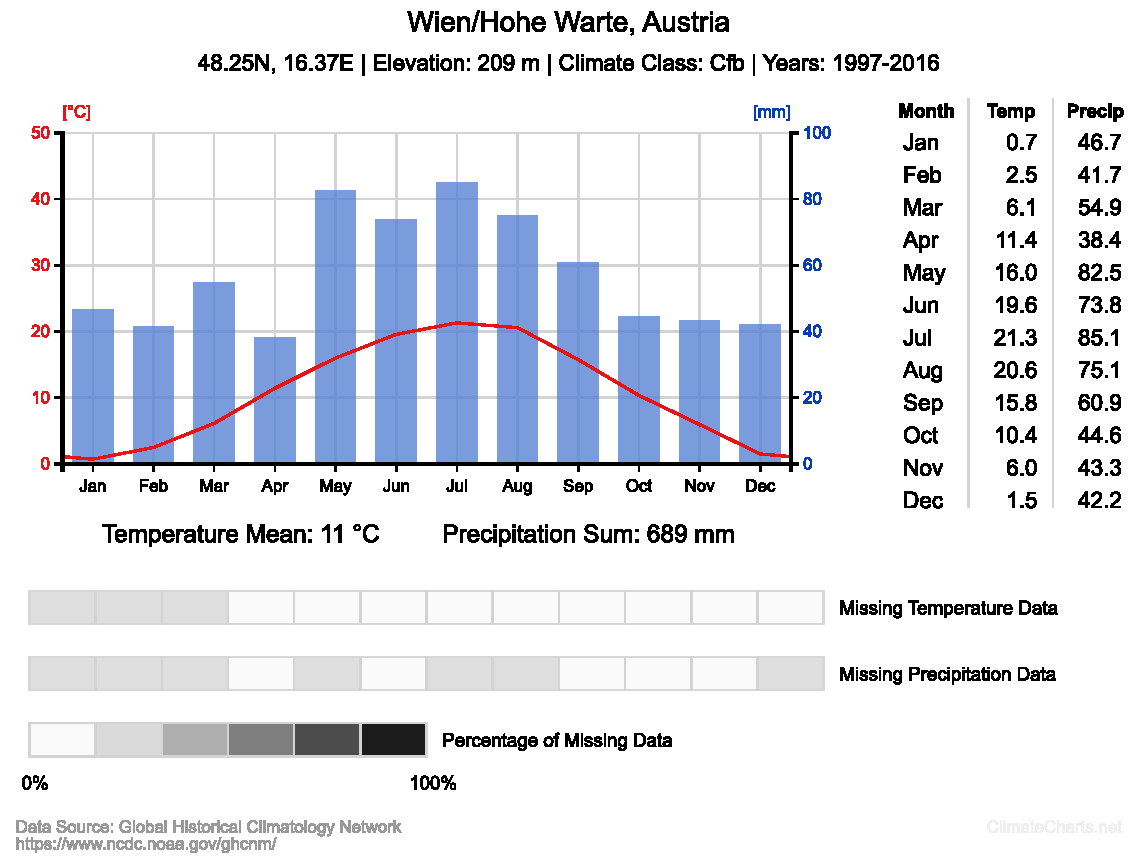
\includegraphics[width = 0.96\textwidth]{temp_maps/temp_vienna}
  	\caption{Monthly averages of temperature and precipitation data for the Hohe Warte in Vienna, Austria. (Image credit: \cite{Zepner:2020})}
	\label{fig:temp_vienna}
\end{figure}

Building on the previous findings, the electrical power output of a PV generator can be calculted by using one of the following equations:
	\begin{equation} \label{eq:p_pv_i}
	\centering
		P_{\mathrm{PV}}(I_{\mathrm{PV}}, \vartheta_{\mathrm{C}}, \Phi_{\mathrm{G}}) = m \, N_{\mathrm{C}} \, U_{\mathrm{T}} \, I_{\mathrm{PV}} \, \ln \left( \frac{I_{\mathrm{Ph}} - I_{\mathrm{PV}} + I_{\mathrm{S}}}{I_{\mathrm{S}}} \right) \text{,}
	\end{equation}
	\begin{equation} \label{eq:p_pv_u}
	\centering
		 P_{\mathrm{PV}}(U_{\mathrm{PV}}, \vartheta_{\mathrm{C}}, \Phi_{\mathrm{G}}) = U_{\mathrm{PV}} \left[ I_{\mathrm{Ph}} - I_{\mathrm{S}} \left( \exp \left(\frac{U_{\mathrm{PV}}}{m \, N_{\mathrm{C}} \, U_{\mathrm{T}} } \right) - 1  \right) \right] \text{.}
	\end{equation}
Typically, $P_{\mathrm{PV}}$ is plotted as a function of $U_{\mathrm{PV}}$, which results in a curve as shown in the figure \ref{fig:tikz_PVG_power_curve} \cite{Prechtl:2006, Mertens:2015, Wagner:2018}.
\begin{figure}[h!]
	\centering
	\input{tikz/tikz_PVG_power_curve}
	\caption{Electrical power output of a photovoltaic generator as a function of $U_{\mathrm{PV}}$. It is further dependent on the photovoltaic cell temperature $\vartheta_{\mathrm{C}}$ and the radiation flux $\Phi_{\mathrm{G}}$. (Recreated from: \cite{Mertens:2015})}
	\label{fig:tikz_PVG_power_curve}
\end{figure}
\subsection{MPP tracking solar charging controllers}
The aim of a SCC is to distribute a PV generator's electrical energy to supply one or more electrical consumers and to recharge an electrochemical energy storage device. The latter is required to supply electrical consumers during times without sunlight. SCCs that can track the MPP of a PV generator, thus providing the greatest electrical energy to the load and the electrochemical energy storage device (compare to figure \ref{fig:tikz/tikz_solar_energy_distribution}), determine the current $I_{\mathrm{MPP}}(\vartheta_{\mathrm{C}}, \Phi_{\mathrm{G}})$ and voltage $U_{\mathrm{MPP}}(\vartheta_{\mathrm{C}}, \Phi_{\mathrm{G}})$. This can be accomplished by analyzing the equation (\ref{eq:p_pv_i}) from which the derivative of $P_{\mathrm{PV}}(I_{\mathrm{PV}}, \vartheta_{\mathrm{C}}, \Phi_{\mathrm{G}})$, with respect to $I_{\mathrm{PV}}$, results in the equation (\ref{eq:dp_pv}).
	\begin{equation} \label{eq:dp_pv}
	\centering
		 \dfrac{\mathrm d P_{\mathrm{PV}}(I_{\mathrm{PV}}, \vartheta_{\mathrm{C}}, \Phi_{\mathrm{G}})}{\mathrm d I_{\mathrm{PV}}} = m \, N_{\mathrm{C}} \, U_{\mathrm{T}} \left( \ln \left( \frac{I_{\mathrm{Ph}} - I_{\mathrm{PV}} + I_{\mathrm{S}}}{I_{\mathrm{S}}} \right) - \frac{I_{\mathrm{PV}}}{I_{\mathrm{Ph}} - I_{\mathrm{PV}} + I_{\mathrm{S}}} \right)
	\end{equation}
Since the slope of the curve $P_{\mathrm{PV}}(I_{\mathrm{PV}}, \vartheta_{\mathrm{C}}, \Phi_{\mathrm{G}})$ becomes $0\mathrm{V}$ for its maxima, $I_{\mathrm{PV}} = I_{\mathrm{MPP}}$ applies as shown below:
	\begin{equation} \label{eq:dp_pv_zero}
	\centering
		 m \, N_{\mathrm{C}} \, U_{\mathrm{T}} \left( \ln \left( \frac{I_{\mathrm{Ph}} - I_{\mathrm{MPP}} + I_{\mathrm{S}}}{I_{\mathrm{S}}} \right) - \frac{I_{\mathrm{MPP}}}{I_{\mathrm{Ph}} - I_{\mathrm{PV}} + I_{\mathrm{S}}} \right) = 0\mathrm{V} \text{.}
	\end{equation}
If now the equation (\ref{eq:dp_pv_zero}) is subtracted from the equation (\ref{eq:u_of_i}) for the case $U_{\mathrm{PV}}(I_{\mathrm{MPP}}, \vartheta_{\mathrm{C}}, \Phi_{\mathrm{G}}) = U_{\mathrm{MPP}}(\vartheta_{\mathrm{C}}, \Phi_{\mathrm{G}})$, the voltage at MPP can be rewritten as follows \cite{Mertens:2015, Wagner:2018}:
	\begin{equation} \label{eq:u_mpp_i_mpp}
	\centering
		 U_{\mathrm{MPP}}(I_{\mathrm{MPP}}, \vartheta_{\mathrm{C}}, \Phi_{\mathrm{G}}) = \frac{m \, N_{\mathrm{C}} \, U_{\mathrm{T}} \, I_{\mathrm{MPP}}}{I_{\mathrm{Ph}} - I_{\mathrm{MPP}} + I_{\mathrm{S}}} \text{.}
	\end{equation}

In addition to the equation (\ref{eq:p_mpp}), $P_{\mathrm{MPP}}(\vartheta_{\mathrm{C}}, \Phi_{\mathrm{G}})$ can directly be obtained from $\Phi_{\mathrm G}$ as presented in the equation (\ref{eq:p_mpp_phi_temp}). For this, however, the PV generator's \emph{efficiency} $\eta_{\mathrm{PV}}$ in $\left(1\right)$ and its temperature coefficient $\mathrm{TC}(P_{\mathrm{MPP}})$ in $\left( \% ^\circ \mathrm{C}^{-1}\right)$ for the electrical power output at MPP must be known.\footnote{Typical $\mathrm{TC}(P_{\mathrm{MPP}})$ values for Si-PV cells are around $-0,4$ to $-0,5$ $\% ^\circ \mathrm{C}^{-1}$.} These quantities can be found in the data sheet of a PV generator. 
	\begin{equation} \label{eq:p_mpp_phi_temp}
	\centering
		 P_{\mathrm{MPP}}(\vartheta_{\mathrm{C}}, \Phi_{\mathrm{G}}) = \eta_{\mathrm{PV}} \, \Phi_{\mathrm G} \left[ 1 + \frac{\mathrm{TC}(P_{\mathrm{MPP}})}{100\%} \left(\vartheta_{\mathrm{C}} - \vartheta_{\mathrm{STC}} \right) \right]
	\end{equation}
Alternatively, $\eta_{\mathrm{PV}}$ can be calculated by using the equation (\ref{eq:p_mpp_phi_temp}) and the table \ref{tab:table_STC}, while regarding the expression $P_\mathrm{MPP,STC} = U_\mathrm{MPP,STC} \, I_\mathrm{MPP,STC}$. This is because $\eta_{\mathrm{PV}}$ depends exclusively on the material and the structure of a PV cell. Moreover, it is assumed that the PV cell is ideal and that every photon which hits the semiconductor and fulfills $W_{\mathrm{Ph}} > \Delta W_{\mathrm{gap}}$, is absorbed and leads to an electron which contributes to $I_\mathrm{Ph}$. In the mentioned inequality $W_{\mathrm{Ph}}$ is the \emph{energy of a photon} in $\left(\mathrm{eV}\right)$ and $\Delta W_{\mathrm{gap}}$ is the \emph{band gap} in $\left(\mathrm{eV}\right)$ of the semiconductor \cite{Mertens:2015, Wagner:2018}.

With the equations (\ref{eq:p_mpp}), (\ref{eq:u_mpp_i_mpp}) and (\ref{eq:p_mpp_phi_temp}), the PV generator's current at MPP can be converted into the following quadratic equation:
	\begin{equation} \label{eq:i_mpp_quadratic}
	\centering
		 I_{\mathrm{MPP}}^2 + c_{\mathrm{PV}} \, I_{\mathrm{MPP}} - c_{\mathrm{PV}} \left(I_{\mathrm{Ph}} + I_{\mathrm{S}}\right) = 0\mathrm{A}^2 \text{, }
	\end{equation}
with $c_{\mathrm{PV}}$ being:
	\begin{equation} \label{eq:c_pv}
	\centering
		 c_{\mathrm{PV}} = \dfrac{\eta_{\mathrm{PV}} \, \Phi_{\mathrm G} \left[ 1 + \dfrac{\mathrm{TC}(P_{\mathrm{MPP}})}{100\%} \left(\vartheta_{\mathrm{C}} - \vartheta_{\mathrm{STC}} \right) \right]}{m \, N_{\mathrm{C}} \, U_{\mathrm{T}}} \text{.}
	\end{equation}
Finally, $I_{\mathrm{MPP}}(\vartheta_{\mathrm{C}}, \Phi_{\mathrm{G}})$ can be solved to:
	\begin{equation} \label{eq:i_mpp_sqr_root}
	\centering
		 I_{\mathrm{MPP}}(\vartheta_{\mathrm{C}}, \Phi_{\mathrm{G}}) = \sqrt{\frac{c_{\mathrm{PV}}^2}{4} + c_{\mathrm{PV}} \left(I_{\mathrm{Ph}} + I_{\mathrm{S}}\right)} - \frac{c_{\mathrm{PV}}}{2} \text{.}
	\end{equation}
The PV generator's voltage at MPP can consequently be calculated using the equation (\ref{eq:i_of_u}) for the case $U_{\mathrm{PV}}(I_{\mathrm{MPP}}, \vartheta_{\mathrm{C}}, \Phi_{\mathrm{G}})$, or using the equation (\ref{eq:u_mpp_i_mpp}).

Due to the fact that real MPP tracking SCCs do not have information about the connected PV generator, a \emph{shunt resistor} $R_\mathrm{shunt}$ in $\left( \Omega \right)$ is used to find the MPP. A charging- and MPP-controller inside the SCC then controls the \emph{duty cycle} $a$ in $\left( \% \right)$ of a DC/DC converter, so that the load and the electrochemical energy storage device are supplied with the greatest electrical energy. An illustration of the basic structure of such a MPP tracking SCC can be seen in the figure \ref{fig:tikz_SCC}. $I_\mathrm{SCC}$ in $\left(\mathrm{A}\right)$ is the current that is consumed by the charging- and MPP-controller \cite{Mertens:2015}. 
\begin{figure}[h!]
	\centering
	\input{tikz/tikz_SCC}
	\caption{The basic structure of a maximum power point tracking solar charging controller. (Recreated from: \cite{Mertens:2015})}
	\label{fig:tikz_SCC}
\end{figure}




\subsection{Electrochemical energy storage} \label{sec:electrochemical}
In order to guarantee a constant supply of electrical energy during times when the PV generator cannot supply the self-sufficient voice communication system, an electrochemical energy storage device is required. Such storage devices are typically rechargeable batteries -- consisting of secondary cells -- based on either lithium, sodium, nickel or lead \cite{Mertens:2015, Sterner:2017, Kurzweil:2018}. 

\emph{Nickel-cadmium} ($\mathrm{NiCd}$) and \emph{nickel-hydrogen} ($\mathrm{NiH}_2$) batteries have long been used for aerospace applications. However, in recent years they have been increasingly replaced by lithium-ion batteries \cite{Ley:2011}. This is due to their high energy density and low self-discharge. On the other hand, the main disadvantages of lithium-ion batteries are high acquisition costs, the need for a \emph{battery management system} (BMS) to maintain safe operation and the strong dependency of the battery performance on the ambient temperatur $\vartheta_{\mathrm{A}}$. The latter becomes a problem only at extreme ambient temperatures \cite{Hausmann:2013, Wehbe:2015, Ala-A.-Hussein:2015, Nejad:2016, Chin:2018}.

In terms of safe operation, \emph{lithium iron phosphate} ($\mathrm{LiFePO}_4$) batteries are among the safest lithium-ion batteries available today. They are furthermore non-toxic\footnote{Compared to, for example, \emph{lithium cobalt oxide} ($\mathrm{LiCoO}_2$) batteries.} and have a very constant cell voltage for different charging states (see linear part in figure \ref{fig:tikz_u_oc_vs_soc}). It is noted that for the \emph{state of charge} $\mathrm{SOC} = 1$ the battery is fully charged and for $\mathrm{SOC} = 0$ it is fully discharged  \cite{Mertens:2015, Sterner:2017, Li:2018, Kurzweil:2018, Hinz:2019, Hossain:2019, Offgridtec:2020}. 

Because $\mathrm{LiFePO}_4$ batteries are commercially available and often used with photvoltaic standalone systems, this subsection aims to model the \emph{terminal voltage} $U_\mathrm{B} = U_\mathrm{B}(\mathrm{SOC})$ in $\left( \mathrm{V} \right)$ of such a battery for a given current $I_\mathrm{B} = I_\mathrm{B}(t)$, based on an experimental approach \cite{Mertens:2015, Offgridtec:2020}. For this purpose, $I_\mathrm{B}(t)$ is defined as shown below:
	\begin{equation} \label{eq:battery_current}
		\centering
		I_\mathrm{B}(t) =
  		\begin{cases}
   			I_\mathrm{D}(t)\text{,} & \text{when discharging the battery} \\
    		- I_\mathrm{C}(t)\text{,} & \text{when charging the battery.}
  		\end{cases}
	\end{equation} 
	
Following from the equation (\ref{eq:battery_current}), the $\mathrm{SOC}$ of a battery as a function of the discharge or charge \emph{time} $t$ in $\left(\mathrm{h}\right)$ can be calculated directly from the \emph{Coulomb counting method} in the equation (\ref{eq:soc}). 
	\begin{equation} \label{eq:soc}
		\centering
		\begin{gathered}
		\mathrm{SOC}(t) = \mathrm{SOC}_\mathrm{init} - \dfrac{\eta_\mathrm{C}}{Q_\mathrm{tot}} \int\limits_{0\mathrm{h}}^{t} I_\mathrm{B}(\tau) \,\mathrm{d}\tau \\
		\mathrm{SOC}(t) = \mathrm{SOC}_\mathrm{init} - \dfrac{\eta_\mathrm{C}}{Q_\mathrm{tot}} \displaystyle\sum_{\tau = 0\mathrm{h}}^{t} I_\mathrm{B}(\tau) \, \Delta \tau
		\end{gathered}
	\end{equation} 
$\mathrm{SOC}_\mathrm{init}$ in $\left(1\right)$ is the \emph{initial} SOC of the battery. It can be calculated by the ratio of the \emph{remaining battery charge} $Q_\mathrm{rem}$ in $\left(\mathrm{Ah}\right)$ to the \emph{total available battery charge} $Q_\mathrm{tot}$ in $\left(\mathrm{Ah}\right)$ as written in the equation (\ref{eq:soc_init}). $\eta_\mathrm{C}$ is the \emph{coulombic efficiency} in $\left(1\right)$ for which $\eta_\mathrm{C} = 1$ applies when discharging and $\eta_\mathrm{C} \leq 1$ applies when charging \cite{He:2011, Wehbe:2015, Nejad:2016, Kurzweil:2018, Li:2018}. In the proposed model it is assumed that $\eta_\mathrm{C} = 1$ applies for both cases \cite{Hentunen:2014, Hinz:2019,Gurjer:2019}.
	\begin{equation} \label{eq:soc_init}
	\centering
		\mathrm{SOC}_\mathrm{init} = \dfrac{Q_\mathrm{rem}}{Q_\mathrm{tot}}
	\end{equation}

According to the authors of \cite{Hausmann:2013, Kurzweil:2018, Saldana:2019}, the total available battery charge $Q_\mathrm{tot}$ when discharging depends on the \emph{discharging current} $I_\mathrm{D}$ in $\left(\mathrm{A}\right)$. During charging -- with the \emph{charging current} $I_\mathrm{C}$ in $\left(\mathrm{A}\right)$ -- $Q_\mathrm{tot}$ is equal to the \emph{nominal battery charge} $Q_\mathrm{nom}$ in $\left(\mathrm{Ah}\right)$. This empirical approximation is summarized in the equation (\ref{eq:battery_charge}), in which $k_\mathrm{P} \approx 1,05$ is the \emph{Peukert constant} for lithium-ion batteries and $Q_\mathrm{nom}$ can be taken from the data sheet of a $\mathrm{LiFePO}_4$ battery \cite{Hausmann:2013, Kurzweil:2018}.
	\begin{equation} \label{eq:battery_charge}
	\centering
		Q_\mathrm{tot} \approx
  		\begin{cases}
   			Q_\mathrm{nom} \left(\dfrac{I_\mathrm{nom}}{I_\mathrm{D}}\right)^{k_\mathrm{P} - 1} \text{,} & \text{when discharging the battery} \\
    		Q_\mathrm{nom}\text{,} & \text{when charging the battery}
  		\end{cases}
	\end{equation} 
	
Since $Q_\mathrm{nom}$ depends on the \emph{discharging rate} $\mathrm{C_D}$ in $\left(\mathrm{h}^{-1}\right)$, which is listed in the data sheet as well, the \emph{nominal battery current} $I_\mathrm{nom}$ in $\left(\mathrm{A}\right)$ can be calculated as follows \cite{Thirugnanam:2014, Kurzweil:2018}: 
	\begin{equation} \label{eq:i_nom}
	\centering
		I_\mathrm{nom} = \mathrm{C_D} \, Q_\mathrm{nom} \text{.}
	\end{equation}
	
From the above it can now be concluded that the \emph{battery charge} as a function of the time $Q_\mathrm{B}(t)$ in $\left(\mathrm{Ah}\right)$ must result in:
\begin{equation} \label{eq:q_b}
\centering
	Q_\mathrm{B}(t) = \mathrm{SOC} \, Q_\mathrm{tot} \text{.}
\end{equation}

The simplest EEC model of a $\mathrm{LiFePO}_4$ battery is an ideal voltage source. Altough this model is easy to implement and compute in simulations, it lacks important properties such as the dynamical behavior of the battery's open-circuit voltage $U_0 = U_0(\mathrm{SOC})$ in $\left( \mathrm{V} \right)$, \emph{electrolyte resistance} when discharging $R_{\mathrm{e,D}} = R_{\mathrm{e,D}}(\mathrm{SOC})$ in $\left( \Omega \right)$ and electrolyte resistance when charging $R_{\mathrm{e,C}} = R_{\mathrm{e,C}}(\mathrm{SOC})$ in $\left( \Omega \right)$. To incorporate these properties and improve accuracy while keeping the model simple, the $R_{\mathrm{int}}$ model shown in the figure (\ref{fig:tikz_simple_battery_model}) is used. The diodes in this model are assumed to be ideal and are only present to illustrate which resistor is used depending on the sign of $I_\mathrm{B}$ \cite{He:2011, Wehbe:2015, Hinz:2019, Saldana:2019}. 
\begin{figure}[h!]
	\centering
	\input{tikz/tikz_simple_battery_model}
	\caption{$R_{\mathrm{int}}$ model of a $\mathrm{LiFePO}_4$ battery (electrochemical energy storage device). (Recreated from: \cite{Hinz:2019, Saldana:2019})}
	\label{fig:tikz_simple_battery_model}
\end{figure}

Figure \ref{fig:tikz_u_oc_vs_soc} shows the typical behavior of the open-circuit voltage $U_0$ of a $\mathrm{LiFePO}_4$ battery as a function of the $\mathrm{SOC}$. For the electrolyte resistances $R_{\mathrm{e,D}}(\mathrm{SOC})$ and $R_{\mathrm{e,C}}(\mathrm{SOC})$, however, it is more difficult to create a generalized function curve. This is due to their varying behavior for different $\mathrm{LiFePO}_4$ batteries \cite{Mertens:2015, Sterner:2017, Li:2018, Hinz:2019, Hossain:2019}. 
\begin{figure}[h!]
	\centering
	\input{tikz/tikz_u_oc_vs_soc}
	\caption{Typical behavior of the open-circuit voltage $U_0$ of a $\mathrm{LiFePO}_4$ battery depending on the $\mathrm{SOC}$. $\mathrm{SOC_1}$ to $\mathrm{SOC}_{N_\mathrm{MP}}$ represent the measuring points for the discharging and charging experiment. (Recreated from: \cite{Mertens:2015, Sterner:2017, Li:2018, Hinz:2019, Hossain:2019})}
	\label{fig:tikz_u_oc_vs_soc}
\end{figure}

On this basis, the terminal voltage of the battery $U_\mathrm{B}$ as a function of the SOC, and wether it is being discharged or charged, can be obtained after Kirchhoff's second law is applied to the model \cite{He:2011, Wehbe:2015, Hinz:2019, Saldana:2019}:
	\begin{equation} \label{eq:battery_voltage}
	\centering
		U_\mathrm{B}(\mathrm{SOC}) =
  		\begin{cases}
   			U_0 - R_{\mathrm{e,D}} \, I_\mathrm{D}\text{,} & \text{when discharging the battery} \\
    		U_0 + R_{\mathrm{e,C}} \, I_\mathrm{C}\text{,} & \text{when charging the battery.}
  		\end{cases}
	\end{equation} 
	
At this point it must be made clear that a $\mathrm{LiFePO}_4$ battery is completely discharged when the voltage $U_\mathrm{B} = U_\mathrm{cut-off}$ is reached and fully charged when the voltage $U_\mathrm{B} = U_\mathrm{full}$ is reached \cite{Hinz:2019, Offgridtec:2020}.\footnote{The name \emph{cuf-off voltage} comes from the fact that the BMS turns off the battery to avoid an unsafe state.} If the equations (\ref{eq:battery_voltage}) and (\ref{eq:battery_charge}) are compared, it can be seen that $U_\mathrm{cut-off}$ is reached at a later point in time for smaller currents $I_\mathrm{D}$. This shows that the battery can be discharged more deeply, which manifests itself in a larger total available battery charge $Q_\mathrm{B}$ \cite{Hausmann:2013, Kurzweil:2018}. Here, however, the compromise is made that the cut-off voltage in the proposed model varies for different discharging currents. 

Figure \ref{fig:tikz_pc_pd_battery_curve} shows the behavior of the battery voltage $U_{\mathrm B}(t)$ when it is discharged with a constant current $I_{\mathrm D}$ over the \emph{time interval} $\Delta t_{\mathrm{D}} = t_\mathrm{D, off} - t_\mathrm{D, on}$ in $\left(\mathrm{h}\right)$ and then charged with the constant current $I_{\mathrm C}$ over the time interval $\Delta t_{\mathrm{C}} = t_\mathrm{C, off} - t_\mathrm{C, on}$ in $\left(\mathrm{h}\right)$ \cite{Rahmoun:2012, Hentunen:2014, Li:2018, Kurzweil:2018, Gurjer:2019, Saldana:2019, Hossain:2019}.
\begin{figure}[h!]
	\centering
	\input{tikz/tikz_pc_pd_battery_curve}
	\caption{Behavior of the battery voltage $U_{\mathrm B}(t)$ when it is first discharged with $I_{\mathrm D}$ and then charged with $I_{\mathrm C}$. From the resulting voltage drop $\Delta U_{\mathrm D}(t_\mathrm{D, on})$ and voltage rise $\Delta U_{\mathrm C}(t_\mathrm{C, on})$, the $R_{int}$ model's electrolyte resistances $R_{e,\mathrm{D}}$ and $R_{e,\mathrm{C}}$ can be calculated. The turquoise curve represents the behavior of the modeled battery voltage. (Recreated from: \cite{Rahmoun:2012, Hentunen:2014, Li:2018, Kurzweil:2018, Gurjer:2019, Saldana:2019, Hossain:2019})}
	\label{fig:tikz_pc_pd_battery_curve}
\end{figure}
From the \emph{dropping voltages} $\Delta U_{\mathrm D}(t_\mathrm{D, on})$ and $\Delta U_{\mathrm C}(t_\mathrm{C, off})$ or \emph{rising voltages} $\Delta U_{\mathrm D}(t_\mathrm{D, off})$ and $\Delta U_{\mathrm C}(t_\mathrm{C, on})$ in $\left( \mathrm{V} \right)$, the $R_{int}$ model's electrolyte resistances $R_{\mathrm{e,D}}$ and $R_{\mathrm{e,C}}$ can be calculated as shown in the equations (\ref{eq:r_0_d}) and (\ref{eq:r_0_c}) \cite{Rahmoun:2012, Hentunen:2014, Kurzweil:2018, Gurjer:2019}. 
\begin{equation}\label{eq:r_0_d}
	\centering
	R_{\mathrm{e,D}}(t) = \left|\dfrac{\Delta U_{\mathrm D}}{I_{\mathrm D}}\right|
\end{equation}
\begin{equation}\label{eq:r_0_c}
	\centering
	R_{\mathrm{e,C}}(t) = \left|\dfrac{\Delta U_{\mathrm C}}{I_{\mathrm C}}\right|
\end{equation}
For comparison, the thin turquoise curve represents the behavior of the $R_\mathrm{int}$ model for the same discharge and charge currents $I_{\mathrm D}$ and $I_{\mathrm C}$. At times $t_\mathrm{D, on}$, $t_\mathrm{D, off}$, $t_\mathrm{C, on}$ and $t_\mathrm{C, off}$ it has the same dropping and rising voltages $\Delta U_{\mathrm D}$ and $\Delta U_{\mathrm C}$ as $U_{\mathrm B}(t)$ \cite{Saldana:2019}.

Based on the findings in the articles \cite{Hausmann:2013, Ala-A.-Hussein:2015, Nejad:2016, Chin:2018} it is assumed that $U_0$,  $R_{e,\mathrm{D}}$ and $R_{e,\mathrm{C}}$ do not dependent on the ambient temperature $\vartheta_{\mathrm{A}}$ in the range from $5^\circ \mathrm{C}$ to $45^\circ \mathrm{C}$. Therefore, the proposed model does not apply to temperatures below $5^\circ \mathrm{C}$ and above $45^\circ \mathrm{C}$.

In order to complete the $R_{\mathrm{int}}$ model, the missing properties $U_0(\mathrm{SOC})$, $R_{\mathrm{e,D}}(\mathrm{SOC})$ and $R_{\mathrm{e,C}}(\mathrm{SOC})$ must be determined experimentally. For this purpose, two separate experiments must be carried out as explained in the following paragraphs.

\paragraph*{Discharging experiment:} %% PD EXPERIMENT
The experiment is carried out at the ambient temperature $\vartheta_\mathrm{A} = 25^\circ \mathrm{C}$ with an initially fully charged $\mathrm{LiFePO}_4$ battery ($\mathrm{SOC}_{N_\mathrm{MP}} = 1$) and repeated for the desired \emph{number of measuring points} $N_{\mathrm{MP}}$ in $\left( 1 \right)$, as illustrated in the figure \ref{fig:tikz_u_oc_vs_soc}, until the battery is fully discharged ($\mathrm{SOC}_{1} = 0$) \cite{Rahmoun:2012, Hentunen:2014, Gurjer:2019}. 

A simple measurement setup for this experiment can be seen in the figure \ref{fig:tikz_experiment_1}. $U_\mathrm{shunt}$ in $\left(\mathrm{V}\right)$ is the voltage drop across the shunt resistor $R_\mathrm{shunt}$, measured with \emph{channel 2} (Ch2) of the oscilloscope. On the basis of this voltage drop, $I_\mathrm{L}$ is set so that the battery is discharged with the current:
\begin{equation}\label{eq_i_d_real}
	\centering
I_\mathrm{D} = \dfrac{U_\mathrm{shunt}}{R_\mathrm{shunt}} + I_\mathrm{Ch1} + I_\mathrm{Ch2} \text{.}
\end{equation}
The \emph{measuring currents} $I_\mathrm{Ch1}$ and $I_\mathrm{Ch2}$ in $\left(\mathrm{A}\right)$ caused by the internal resistances of the channels of the oscilloscope are small compared to the load current $I_\mathrm{L}$. Depending on the desired accuracy, $I_\mathrm{Ch1}$ and $I_\mathrm{Ch2}$ can either be neglected or determined by measuring the internal resistances of said channels \cite{Schrufer:2014}.  
\begin{figure}[h!]
	\centering
	\input{tikz/tikz_experiment_1}
	\caption{Measurement setup for the discharge experiment.}
	\label{fig:tikz_experiment_1}
\end{figure}

For a certain measuring point $n \in \mathbb{N}$, the battery's open-circuit voltage $U_{0, \mathrm{D}}(\mathrm{SOC}_n)$ in $\left(\mathrm{V}\right)$ is measured with \emph{channel 1} (Ch1) of the oscilloscope. The battery is then discharged using an electronic load in \emph{constant current} (CC) mode\footnote{Even if the battery voltage slowly drops during the course of the experiment, the electronic load will keep the current constant.} with $I_{\mathrm D}$ for $\Delta t_{\mathrm{D}}$ until the desired new measuring point $\mathrm{SOC}_{n-1}$ is reached. At the point in time when the electronic load is switched on, the voltage drop $\Delta U_{\mathrm D}(\mathrm{SOC}_n)$ is measured with Ch1 and the voltage drop $U_\mathrm{shunt}(\mathrm{SOC}_n)$ with Ch2. After the discharge process for $\Delta t_{\mathrm{D}}$ has been completed, the battery must remain idle for the \emph{resting period} $t_\mathrm{rest}$ in $\left( \mathrm{h} \right)$ until the open-circuit voltage has reached an end value (compare to figure \ref{fig:tikz_pc_pd_battery_curve}). When it is reached, the measurements can be repeated for $\mathrm{SOC}_{n-1}$. For the measuring point $\mathrm{SOC}_1$, the load current $I_\mathrm{L}$ can be switched off immediately after the voltage drop $\Delta U_{\mathrm D}$, so that the BMS does not have to switch off the secondary cells \cite{Rahmoun:2012, Hentunen:2014, Gurjer:2019}.

From the Coulomb counting method, the time interval $\Delta t_{\mathrm{D}}$, which in the course of the experiment can be measured with a timer, and the measuring points can be calculated as follows \cite{He:2011, Wehbe:2015, Nejad:2016, Kurzweil:2018, Li:2018}:
\begin{equation} \label{eq:delta_t_D}
	\centering
	\Delta t_{\mathrm{D}} = \dfrac{ Q_\mathrm{tot}}{\eta_\mathrm{C} \, I_\mathrm{D} \left( N_\mathrm{MP} - 1 \right)} \text{.}
\end{equation}
\begin{equation} \label{eq:SOC_n_minus_1}
	\centering
	\mathrm{SOC}_{n - 1} = \mathrm{SOC}_{n} - \dfrac{\eta_\mathrm{C} \, I_\mathrm{D}}{Q_\mathrm{tot}} \, \Delta t_{\mathrm{D}} \text{.}
\end{equation}

Finally, if $\Delta U_{\mathrm D}$ and $U_\mathrm{shunt}$ are known for the measuring points $\mathrm{SOC}_1$ to $\mathrm{SOC}_{N_{\mathrm{MP}}}$, the resistance $R_{e,\mathrm{D}}$ can be calculated by using the equation (\ref{eq:r_0_d_soc}) -- which is derived from the equations (\ref{eq:r_0_d}) and (\ref{eq_i_d_real}) \cite{Rahmoun:2012, Hentunen:2014, Kurzweil:2018, Gurjer:2019}.
\begin{equation}\label{eq:r_0_d_soc}
	\centering
	R_{\mathrm{e,D}}(\mathrm{SOC}_n) = \left|\dfrac{\Delta U_{\mathrm D}(\mathrm{SOC}_n)}{\dfrac{U_\mathrm{shunt}(\mathrm{SOC}_n)}{R_\mathrm{shunt}} + I_\mathrm{Ch1} + I_\mathrm{Ch2}}\right|
\end{equation}

\paragraph*{Charging experiment:} %% PC EXPERIMENT
Before the course of the experiment is explained, it must first be clarified how a $\mathrm{LiFePO}_4$ battery behaves when charging. Lithium-ion batteries are usually charged with the \emph{constant current}/\emph{constant voltage} (CC/CV) method. As presented in the figure \ref{fig:tikz_cccv_curve}, the battery is first charged with a constant current $I_\mathrm{C}$ for $t_\mathrm{C}$ in $\left(\mathrm{h}\right)$, for which the battery voltage is described with the equation (\ref{eq:battery_voltage}), and then with a constant voltage $U_\mathrm{B}(t) = U_\mathrm{full}$ for $t_\mathrm{V}$ in $\left(\mathrm{h}\right)$. When the charging process is completed, the battery voltage drops to the so called \emph{floating voltage} $U_\mathrm{float}$ in $\left(\mathrm{V}\right)$. This happens when the decreasing charging current $I_\mathrm{B}$ falls below a \emph{minimum current} $I_\mathrm{min}$ in $\left(\mathrm{A}\right)$ \cite{Notten:2005, Mertens:2015, Sterner:2017, Kurzweil:2018, Liu:2020}.
\begin{figure}[h!]
	\centering
	\input{tikz/tikz_cccv_curve}
	\caption{An example of the behavior the battery voltage $U_\mathrm{B}(t)$, battery current $I_\mathrm{B}(t)$ and battery charge $Q_\mathrm{B}(t)$ of a $\mathrm{LiFePO}_4$ battery when it is charged with a constant current $I_\mathrm{C}$ and then with a constant voltage $U_\mathrm{full}$ over a longer period of time. At $t_\mathrm{C} + t_\mathrm{V}$ the battery charger switches from $U_\mathrm{full}$ to $U_\mathrm{float}$ to keep the battery in a fully charged state. (Recreated from: \cite{Notten:2005, Sterner:2017, Liu:2020})}
	\label{fig:tikz_cccv_curve}
\end{figure} 

With the \emph{charge difference} $\Delta Q = Q_\mathrm{tot} - Q_\mathrm{B}(t_\mathrm{C})$ and the model proposed in \cite{Liu:2020}, the battery charge can be written as a function of the charging time as follows: 
\begin{equation} \label{eq:battery_charge_cases}
\centering
		Q_\mathrm{B}(t) =
  		\begin{cases}
   			I_\mathrm{C} \, t \text{,} & \text{for } 0\mathrm{h} \leq t < t_\mathrm{C} 
			\\
    		\Delta Q \left( 1 - \exp \left( -\dfrac{t - t_\mathrm{C}}{\tau_\mathrm{B}} \right) \right) + I_\mathrm{C} \, t_\mathrm{C}\text{,} & \text{for } t_\mathrm{C} \leq t < t_\mathrm{C} + t_\mathrm{V} \text{.}
  		\end{cases}
\end{equation}
It is assumed that $Q_\mathrm{B}(t)$ is continuously differentiable for all points in time. Based on this assumption, the model for the charging current results from the time derivative: 
\begin{equation} \label{current_cases}
\dfrac{\mathrm{d}Q_\mathrm{B}(t)}{\mathrm{d}t} = 
	\left\{\begin{array}{ll}
		I_\mathrm{C}\text{,} & \text{for } 0\mathrm{h} \leq t < t_\mathrm{C} \\[8pt]
		\dfrac{\Delta Q}{\tau_\mathrm{B}} \exp \left( -\dfrac{t - t_\mathrm{C}}{\tau_\mathrm{B}} \right)\text{,} & \text{for } t_\mathrm{C} \leq t < t_\mathrm{C} + t_\mathrm{V}
 	\end{array}\right\} = I_\mathrm{B}(t) \text{.}
\end{equation}
If it is further assumed that $I_\mathrm{B}(t)$ is continuous for all points in time -- therefore does not drop at the point in time $t_\mathrm{C}$ -- the \emph{time constant} $\tau_\mathrm{B}$ in $\left(\mathrm{h}\right)$ of a battery can be obtained from:
\begin{equation}\label{eq:tau_battery}
	\centering
	\tau_\mathrm{B} = \dfrac{\Delta Q}{I_\mathrm{C}}\text{.}
\end{equation}
If -- in the course of the charge experiment -- it can be shown that the second assumption is correct, then the first assumption follows according to \cite{Taschner:2014}.
	
Like the discharge experiment, this experiment is also carried out at $\vartheta_\mathrm{A} = 25^\circ \mathrm{C}$. The $\mathrm{LiFePO}_4$ battery, however, is initially fully discharged ($\mathrm{SOC}_{1} = 0$) and the charging experiment is repeated for the desired number of measuring points $N_{\mathrm{MP}}$ until it is fully charged ($\mathrm{SOC}_{N_\mathrm{MP}} = 1$) \cite{Rahmoun:2012, Hentunen:2014, Gurjer:2019}.

The corresponding measurement setup can be seen in the figure \ref{fig:tikz_experiment_2}. For the currents $I_\mathrm{Ch1}$ and $I_\mathrm{Ch2}$ the same applies as in the discharge experiment since they are small compared to the \emph{battery charger current} $I_\mathrm{BC}$ in $\left(\mathrm{A}\right)$ \cite{Schrufer:2014}.
\begin{figure}[h!]
	\centering
	\input{tikz/tikz_experiment_2}
	\caption{Measurement setup for the charge experiment.}
	\label{fig:tikz_experiment_2}
\end{figure}
Based on the figure \ref{fig:tikz_experiment_2}, the actual charging current $I_\mathrm{C}$ can be calculated with the equation (\ref{eq:i_c_real}).
\begin{equation}\label{eq:i_c_real}
	\centering
I_\mathrm{C} = -\dfrac{U_\mathrm{shunt}}{R_\mathrm{shunt}} - I_\mathrm{Ch1} - I_\mathrm{Ch2}
\end{equation}

Identical to the discharge experiment, the battery's open-circuit voltage $U_{0, \mathrm{C}}(\mathrm{SOC}_n)$ in $\left(\mathrm{V}\right)$ is measured with Ch1. The battery is then charged using a suitable battery charger in (CC/CV) mode with a set $I_{\mathrm C}$, $I_\mathrm{min}$, $U_\mathrm{full}$ and $U_\mathrm{float}$. This is done for the time interval $\Delta t_{\mathrm{C}}$ until the new measuring point $\mathrm{SOC}_{n+1}$ is reached. At the point in time when the battery charger is switched on, the voltage rise $\Delta U_{\mathrm C}(\mathrm{SOC}_n)$ is measured with Ch1 and the voltage drop $U_\mathrm{shunt}(\mathrm{SOC}_n)$ with Ch2. After the charge process for $\Delta t_{\mathrm{C}}$ has been completed, the battery must remain idle for $t_\mathrm{rest}$ until the open-circuit voltage has reached an end value (compare to figure \ref{fig:tikz_pc_pd_battery_curve}). When this value is reached, the measurements can be repeated for $\mathrm{SOC}_{n + 1}$ \cite{Rahmoun:2012, Hentunen:2014, Gurjer:2019}. Based on the previously introduced model $\Delta U_{\mathrm C}(\mathrm{SOC}_{N_\mathrm{MP}})$ cannot be obtained. However, by performing the experiment on a commercially available $\mathrm{LiFePO}_4$ battery, it was found that for longer resting periods $t_\mathrm{rest}$, of up to a few hours, it accepts small charging currents $I_{\mathrm C}$ for a short intervall $\Delta t_\mathrm{C}$ even for $\mathrm{SOC}_{N_\mathrm{MP}}$. It is assumed that this is the consequence of the slow -- almost exponential -- decrease of $U_{0, \mathrm{C}}(\mathrm{SOC}_{_\mathrm{MP}})$ (compare to figure \ref{fig:tikz_pc_pd_battery_curve}) \cite{Kurzweil:2018}. In this case, the equation (\ref{eq:battery_voltage}) is not equal to $U_{\mathrm{full}}$ anymore.

To confirm the previously made assumption that $I_{\mathrm C}(t)$ is continuous for all points in time, it is measured with Ch2 and calculated by using the equation (\ref{eq:i_c_real}) \cite{Notten:2005, Mertens:2015, Sterner:2017, Kurzweil:2018, Liu:2020}. 

The time interval $\Delta t_{\mathrm{C}}$ and the measuring points are calculated -- base on the Coulomb counting method -- as shown below \cite{He:2011, Wehbe:2015, Nejad:2016, Kurzweil:2018, Li:2018}:
\begin{equation} \label{eq:delta_t_C}
	\centering
	\Delta t_{\mathrm{C}} = \dfrac{ Q_\mathrm{tot}}{\eta_\mathrm{C} \, I_\mathrm{C} \left( N_\mathrm{MP} - 1 \right)} \text{.}
\end{equation}
\begin{equation} \label{eq:SOC_n_plus_1}
	\centering
	\mathrm{SOC}_{n + 1} = \mathrm{SOC}_{n} + \dfrac{\eta_\mathrm{C} \, I_\mathrm{C}}{Q_\mathrm{tot}} \, \Delta t_{\mathrm{C}} \text{.}
\end{equation}

Similar to $R_{e,\mathrm{D}}$, $R_{e,\mathrm{C}}$ can be obtained -- by using the equations (\ref{eq:r_0_c}) and (\ref{eq:i_c_real}) -- from \cite{Rahmoun:2012, Hentunen:2014, Kurzweil:2018, Gurjer:2019}:
\begin{equation}\label{eq:r_0_c_soc}
	\centering
	R_{\mathrm{e,C}}(\mathrm{SOC}_n) = \left|-\dfrac{\Delta U_{\mathrm C}(\mathrm{SOC}_n)}{\dfrac{U_\mathrm{shunt}(\mathrm{SOC}_n)}{R_\mathrm{shunt}} + I_\mathrm{Ch1} + I_\mathrm{Ch2}}\right| \text{.}
\end{equation}

Due to the hysteresis effects of the open-circuit voltage $U_0(\mathrm{SOC}_n)$ mentioned in \cite{Hentunen:2014, Wehbe:2015, Gurjer:2019, Saldana:2019}, the battery voltage in the equation (\ref{eq:battery_voltage}) must be adapted to the so-called \emph{zero-state hysteresis model}:

\begin{equation} \label{eq:battery_voltage_adapted}
	\centering
		U_\mathrm{B}(\mathrm{SOC}_n) =
  		\begin{cases}
   			U_0 (\mathrm{SOC}_n)+ \dfrac{c_{\mathrm{B}}}{2} - R_{\mathrm{e,D}}(\mathrm{SOC}_n) \, I_\mathrm{D}\text{,} \\ \text{when discharging the battery} \\[8pt]
    		U_0(\mathrm{SOC}_n) + \dfrac{c_{\mathrm{B}}}{2} + R_{\mathrm{e,C}}(\mathrm{SOC}_n) \, I_\mathrm{C}\text{,} \\\text{when charging the battery,}
  		\end{cases}
	\end{equation} 
with: 
\begin{equation} \label{eq:U_0}
	\centering
	U_0(\mathrm{SOC}_n) = \dfrac{U_{0,\mathrm{D}}(\mathrm{SOC}_n) + U_{0,\mathrm{C}}(\mathrm{SOC}_n)}{2}\text{,}
\end{equation}
and $c_{\mathrm{B}}$ depending on the sign of $I_\mathrm{B}$:
\begin{equation} \label{eq:c_B}
	\centering
		c_{\mathrm{B}} =
  		\begin{cases}
   			\left| U_{0, \mathrm{C}}(\mathrm{SOC}_n) - U_{0, \mathrm{D}}(\mathrm{SOC}_n) \right| \cdot (-1) \text{,} & \text{for } I_\mathrm{B} > 0\mathrm{A} \\
			0\text{,} & \text{for } I_\mathrm{B} = 0\mathrm{A} \\
			\left| U_{0, \mathrm{C}}(\mathrm{SOC}_n) - U_{0, \mathrm{D}}(\mathrm{SOC}_n) \right| \text{,} & \text{for } I_\mathrm{B} < 0\mathrm{A}\text{.}
  		\end{cases}
	\end{equation} 



\subsection{Cable losses}
Cables are used to distribute the generated electrical energy in the self-sufficient voice communication system. The transport of the \emph{electrical charge} $Q$ in $\left( \mathrm{As} \right)$ in a cable, however, causes electrical losses which have to be considered with: 
	\begin{equation} \label{eq:p_cable}
	\centering
		 P_\mathrm{loss}(\vartheta_\mathrm{A}) = \left(\dfrac{\mathrm d Q(A)}{\mathrm d t}\right)^2 R_\mathrm{cable}(\vartheta_\mathrm{A}) \text{.}
	\end{equation}
$I(A) = \mathrm d Q(A) / \mathrm d t$ represents the time throughput rate of the electrical charge shifted in a directed manner through the \emph{cross-sectional area} $A$ in $\left( \mathrm{mm}^2 \right)$ of a cable. This corresponds to the electrical current $I$ in $\left( \mathrm{A} \right)$ at the area $A$. The second factor $R_\mathrm{cable}(\vartheta_\mathrm{A})$ in $\left( \Omega \right)$ is the \emph{cable resistance} depending on the ambient temperature $\vartheta_\mathrm{A}$. It can be calculated with the equation (\ref{eq:r_cable}), where $l$ in $\left( \mathrm m \right)$ is the \emph{length} of the cable, $\varrho$ in $\left(\Omega \mathrm{mm}^2\mathrm{m}^{-1}\right)$ is the \emph{specific resistance} and $\alpha$ in $\left( ^\circ \mathrm{C}^{-1} \right)$ is the \emph{temperature coefficient} of the material the cable is made of. $\vartheta_\mathrm{ref}$ in $\left( ^\circ \mathrm{C} \right)$ is the temperature for which $\varrho$ applies.
	\begin{equation} \label{eq:r_cable}
	\centering
		 R_\mathrm{cable}(\vartheta_\mathrm{A}) = \dfrac{\varrho \, l}{A} \, \left[1 + \alpha \left( \vartheta_\mathrm{A} - \vartheta_\mathrm{ref}\right) \right]
	\end{equation}
For example, for $\vartheta_\mathrm{ref} = 20^\circ \mathrm{C}$ copper has a specific resistance of $\varrho_\mathrm{Cu,20} = 0,01673 \Omega \mathrm{mm}^2\mathrm{m}^{-1}$ with a temprature coefficient of $\alpha = {4,3 \cdot 10^{-3}}^\circ \mathrm{C}^{-1}$ \cite{Gerhard-Fasching:2005, Prechtl:2006}. Cable heating by solar radiation is neglected due to the complexity of the subject. 

\subsection{Martian application}
With regard to the usability of the modeled energy distribution for a self-sufficient voice communication system on the surface of Mars, roughly speaking, two main components have to be examined more closely. Namely the PV generator and the $\mathrm{LiFePO}_4$ battery.

Since Mars, with an average distance of $1,524\mathrm{AU}$, is further away from the Sun than the Earth, the solar irradiance $E_\mathrm{S,M}$ in $\left(\mathrm{Wm^{-2}}\right)$ at the top of its atmosphere is $56,9\%$ less than that on Earth \cite{Karttunen:2006}: 
\begin{equation} \label{eq:e_sun_mars}
	\centering
	E_{\mathrm{S,M}} = \frac{\Phi_{\mathrm{S}}}{4 \pi \, \left(1,524 \cdot r_{\mathrm{SE}}\right)^2} = \frac{3,845 \cdot 10^{26} \mathrm{W}}{4 \pi \cdot (2,279871539 \cdot 10^{11} \mathrm{m})^2} = 588,66 \frac{\mathrm{W}}{\mathrm{m}^2}\text{.}
\end{equation}
Similar to the solar resource maps introduced in the subsection \ref{sec:solar_irradiation_on_earths_surface}, the Solar irradiance data collected by NASA's Viking Lander VL1, shown in the figures \ref{fig:image_mars_irradiance_mean} to \ref{fig:image_mars_irradiance_orbit}, can be used to calculate the total generator irradiance on the Martian surface, based on the equations (\ref{eq:e_dni}) and (\ref{eq:e_gen_ghi_dni}):
\begin{equation} \label{eq:e_gen_ghi_dni_mars}
	\centering
		E_{\mathrm{G}}(t_\mathrm{S}) = E_{\mathrm{DHI}} \, \dfrac{\cos \theta}{\sin \gamma_\mathrm{S}} + E_{\mathrm{DIFH}} \,\frac{1 + \cos \beta }{2} + E_{\mathrm{GHI}} \, \frac{1 - \cos \beta }{2} \cdot \mathrm{ALB} \text{.}
\end{equation}
\begin{figure}[h!]
	\centering
  	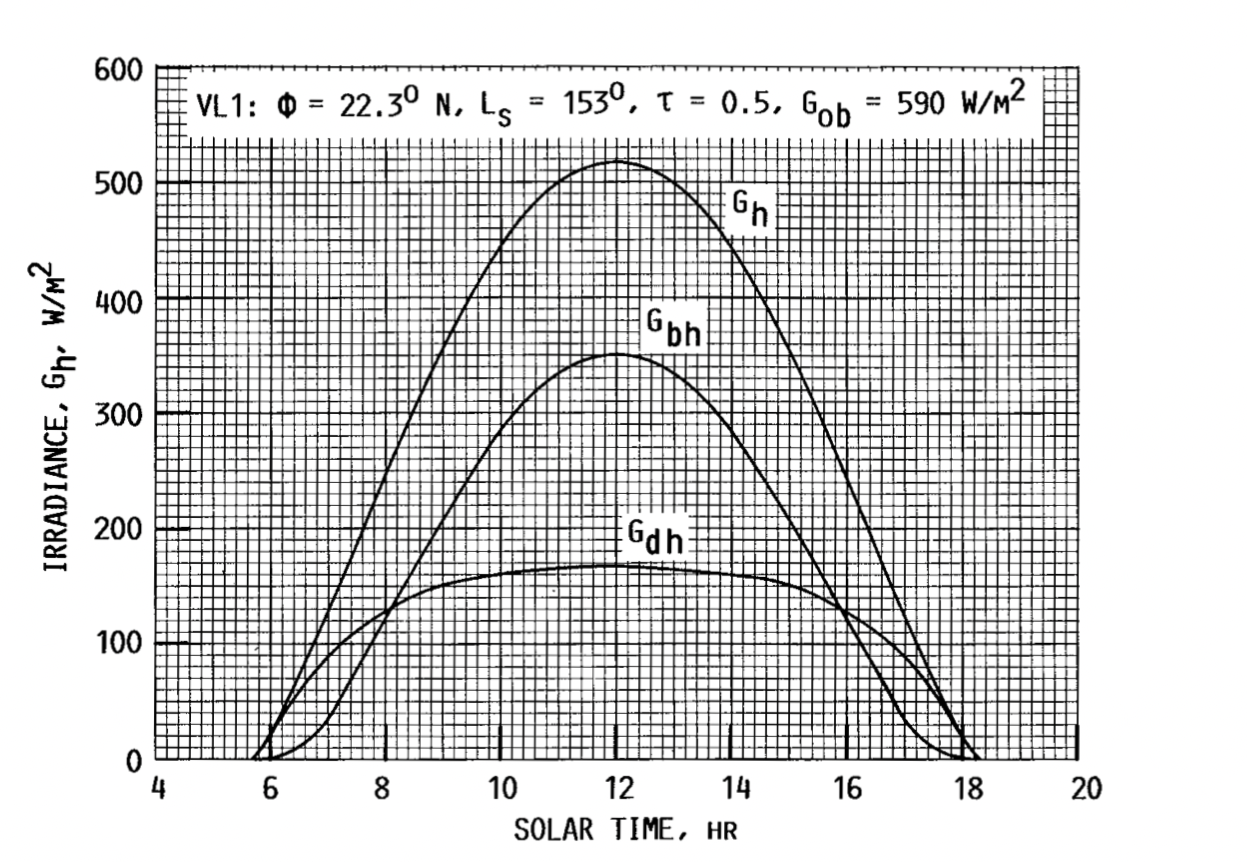
\includegraphics[width = 0.9\textwidth]{images/image_mars_irradiance_mean}
  	\caption{\textit{``Diurnal variation of global $G_\mathrm{h}$, beam $G_\mathrm{bh}$ and diffuse $G_\mathrm{dh}$ irradiance on a horizontal Mars surface at Viking Lander VL1.''} (Image and caption credit: \cite{Appelbaum:1990})}
	\label{fig:image_mars_irradiance_mean}
\end{figure}
The quantities $E_{\mathrm{DHI}}$, $E_{\mathrm{DIFH}}$, $E_{\mathrm{GHI}}$, $\theta$ and $\gamma_\mathrm{S}$ depend on the solar time $t_\mathrm{S}$. As a first approximation, the albedo value $\mathrm{ALB} = 0,25$ can be used. This value represents the mean albedo of Mars \cite{Grayzeck:2020}. In the article \cite{Appelbaum:1990} the authors further state that the albedo of the Martian surface varies in the range of $0,1$ to $0,4$.

The data presented in the figures \ref{fig:image_mars_irradiance_mean} to \ref{fig:image_mars_irradiance_orbit}, however, only applies for the Martian latitude $\phi \ \widehat{=} \ \varphi = 22,3^\circ \, \mathrm{N}$. Figure \ref{fig:image_mars_irradiance_mean} shows the diurnal variation of $E_{\mathrm{DHI}} \ \widehat{=} \ G_\mathrm{bh}$, $E_{\mathrm{DIFH}} \ \widehat{=} \ G_\mathrm{dh}$ and $E_{\mathrm{GHI}} \ \widehat{=} \ G_\mathrm{h}$ on the Martian surface. The quantities $L_\mathrm{S}$, $\tau$ and $G_\mathrm{ob}$ are the areocentric longitude, the optical depth and the beam irradiance at the top of the Martian atmosphere. Similar data is shown in the figures \ref{fig:image_mars_irradiance_orbit} and \ref{fig:image_mars_irradiance_opacity}, but here an additional reference is made to the orbit of Mars around the Sun and the opacity of its atmosphere. For example, the latter can be caused by dust storms \cite{Appelbaum:1990}. 
\begin{figure}[h!]
	\centering
  	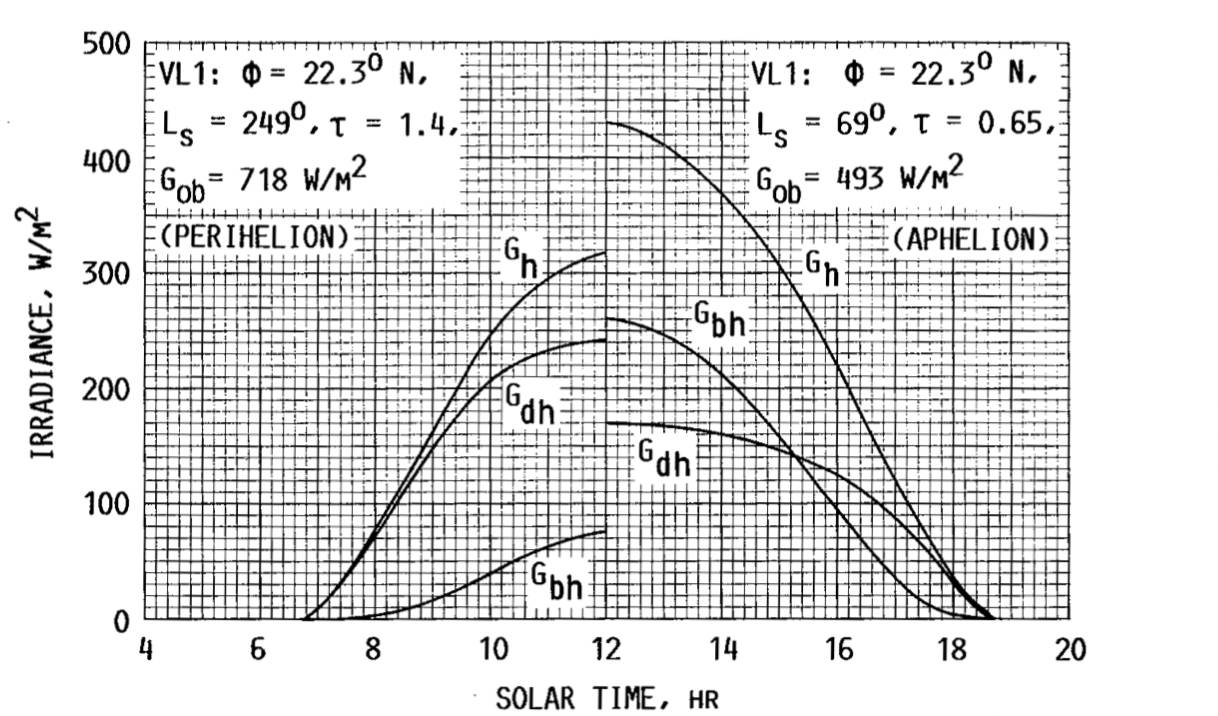
\includegraphics[width = 0.9\textwidth]{images/image_mars_irradiance_orbit}
  	\caption{\textit{``Diurnal variation of global $G_\mathrm{h}$, beam $G_\mathrm{bh}$ and diffuse $G_\mathrm{dh}$ irradiance on a horizontal Mars surface at Viking Lander VL1.''} (Image and caption credit: \cite{Appelbaum:1990})}
	\label{fig:image_mars_irradiance_orbit}
\end{figure}
\begin{figure}[h!]
	\centering
  	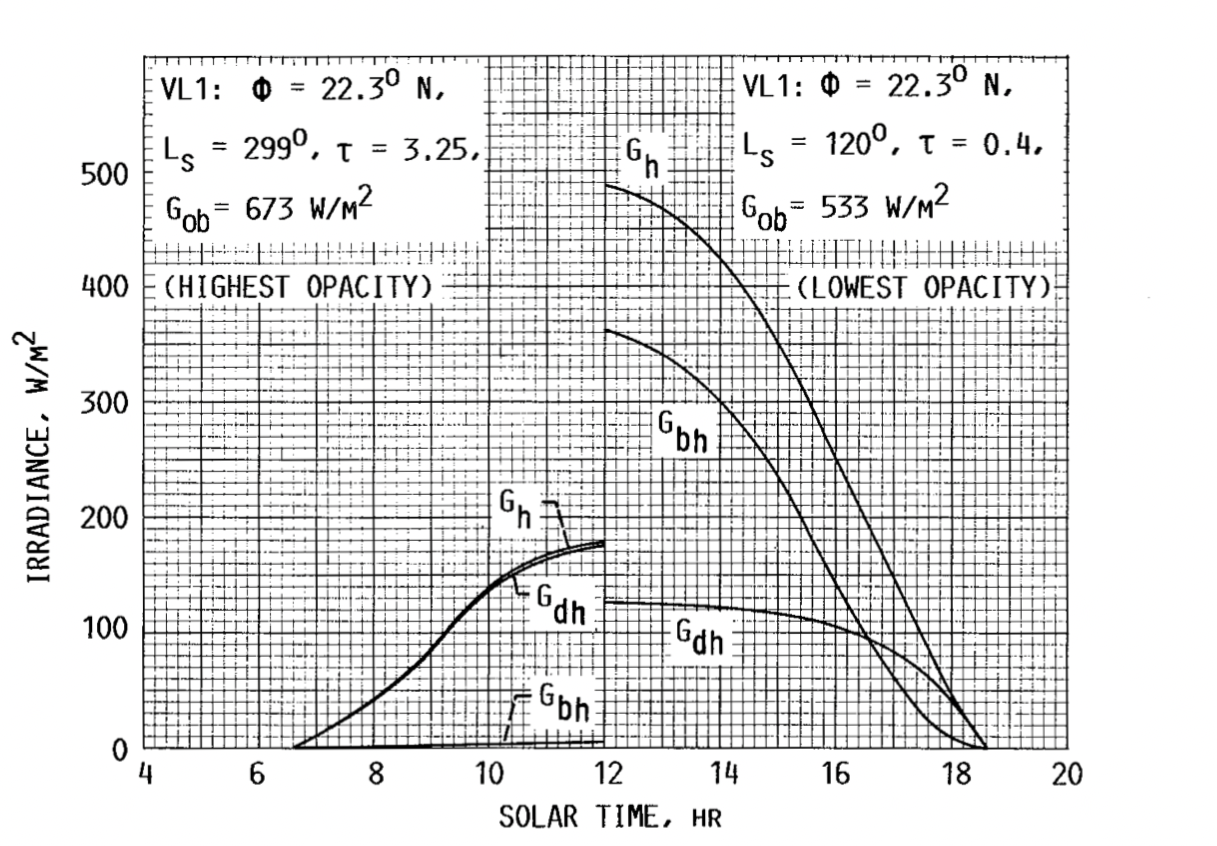
\includegraphics[width = 0.9\textwidth]{images/image_mars_irradiance_opacity}
  	\caption{\textit{``Diurnal variation of global $G_\mathrm{h}$, beam $G_\mathrm{bh}$ and diffuse $G_\mathrm{dh}$ irradiance on a horizontal Mars surface at Viking Lander VL1.''} (Image and caption credit: \cite{Appelbaum:1990})}
	\label{fig:image_mars_irradiance_opacity}
\end{figure}

The angles $\theta$ and $\gamma_\mathrm{S}$ can be calculated with the equations introduced in the subsections \ref{sec:angular_relationships} and \ref{sec:energy_yield}. For these, however, the local latitude $\varphi$, the Sun's declination $\delta$ and the solar time $t_\mathrm{S}$ on Mars must be known. On Mars, the maximum values of $\delta$ are $-25,19^\circ$ and $25,19^\circ$ and the duration of one day is $24,6597\mathrm{h}$ \cite{Grayzeck:2020}. It is noted, that the equations (\ref{eq:delta}) and (\ref{eq:solar_time}) cannot be used to calculate $\delta$ and $t_\mathrm{S}$.

In order to get the same energy yield with a PV generator on Mars as on Earth, this can be achieved in two ways. Based on the equation (\ref{eq:radiation_flux}), and if it is assumed that the PV cell temperatures of the PV generator on Earth and Mars are equal ($\vartheta_\mathrm{C,E} = \vartheta_\mathrm{C,M}$), the radiation flux onto the energy-converting area $A_\mathrm{PV,E}$ of the PV generator on Earth is equal to the radiation flux onto the energy-converting area $A_\mathrm{PV,M}$ of the PV generator on Mars, when the following equation applies:
\begin{equation} \label{eq:pv_area_comparison}
	\centering
		A_{\mathrm{PV,M}} = A_{\mathrm{PV,E}} \, \dfrac{E_{\mathrm{G,E}}}{E_{\mathrm{G,M}}}\text{,} \quad \text{for } \vartheta_\mathrm{C,E} = \vartheta_\mathrm{C,M} \text{.}
\end{equation}
Therefore, a self-sufficient voice communication system with a PV generator area $A_{\mathrm{PV,E}}$ and, for example, the requirement of an annual average irradiance $E_{\mathrm{G,E}}$ to operate on Earth, would require an area $A_{\mathrm{PV,M}}$ if there is an annual avarege irradiance $E_{\mathrm{G,M}}$ at the place of use on Mars. The main disadvantage of this method is, that as the area of the PV generator increases, its mass and thus the payload of a rocket increases. 

Diurnal temperatures between $-89^\circ \mathrm{C}$ to $-31^\circ \mathrm{C}$ on Mars theoretically lead to a higher output power of the PV generator. This can reduce the required area $A_{\mathrm{PV,E}}$ \cite{Mertens:2015, Grayzeck:2020}. However, the influence of temperature must be examined more closely. Altough the ambient temperature is lower, the heat dissipation of the PV generator to the surrounding atmosphere is worse than on Earth \cite{Kemmetmuller:2021}. This shows that the equation (\ref{eq:pv_area_comparison}) can only be used as a rough estimate.

The second approach is based on increasing the sensitivity $S$ of the PV cells (see equation (\ref{eq:sens})) so that equation the (\ref{eq:photo_i}) can still deliver the same photocurrent current to charge the $\mathrm{LiFePO}_4$ battery at a lower radiation flux $\Phi_\mathrm{G}$. In order to achieve this, the structure of the semiconductor the PV cells are made of needs to be adapted and improved. Research is still ongoing in this area \cite{Mertens:2015}.  

With regard to longer lasting dust storms, energy can still be converted to supply the self-sufficient voice communication system due to the diffuse component of the total generator irradiance (compare to figure \ref{fig:image_mars_irradiance_opacity}). This must be planned accordingly \cite{Appelbaum:1990, Appelbaum:1992, Landis:1995, Mertens:2015}. It becomes more complicated when dust collects on the energy-converting area of the PV generator. Crew members would have to dust it off from time to time. This, however, shortens the effective mission time and increases the risk of an accident. Regarding the $\mathrm{LiFePO}_4$ battery, this can further become a problem in between crewed missions. Even though these types of batteries have a low self-discharge, they can get damaged if they are not sufficiently charged for a longer period of time \cite{Offgridtec:2020}.

Finally, the second component that is heavily influenced by the Martian environment is the $\mathrm{LiFePO}_4$ battery. This is mainly due to the aforementioned extreme diurnal ambient temperatures \cite{Hausmann:2013, Wehbe:2015, Ala-A.-Hussein:2015, Nejad:2016, Chin:2018, Grayzeck:2020}. Depending on how well the battery is insulated from the Martian environment in terms of temperature, additional energy from the battery must be used to continuously heat or cool it. Due to this, the nominal battery charge and -- if necessary -- the energy-converting area of the PV generator must be adjusted. 





\section{Voice communication system} \label{sec:link_budget}
In order to establish voice communication -- and at a later stage data communication\footnote{Data communication is not covered in this thesis.} -- it was decided to use the VHF band.\footnote{The VHF band has a frequency range from $30\mathrm{MHz}$ to $300\mathrm{MHz}$.} It is preferred for mobile and handheld radio applications, as the range is relatively short and only extends over a few tens of kilometers. With regard to this, the possible interference with neighboring communication systems can be kept to a minimum \cite{Parsons:2000}. Since the OeWF already uses handheld radios that operate in the VHF band, it was decided to incorporate them into the voice communication system due to their good condition.

In the past, VHF radios mainly used analog modulation methods for signal transmission. Nowadays, however, it is an increasing trend in this industry to use digital modulation methods. These have the decisive advantage that the signal quality -- for example the audio quality -- remains relatively constant up to a certain distance and then deteriorated drastically. In the case of radios that transmit an analog modulated signal, the quality of the signal constantly deteriorates with increasing distance \cite{SystemPlanner:2018}. So that good audio quality over longer distances can be guaranteed the decision was made to use a radio infrastructure based on digital modulation. 

In combination with the aforementioned infrastructure, vertically polarized omnidirectional antennas were preferred because the field strength near the ground is stronger than that of horizontally polarized antennas. Moreover, these antennas are often more convenient to use and their directivity is the same for all cardinal directions -- in relation to the insatallation site of a radio system or the current location of a handheld radio \cite{Parsons:2000}. 

Communication with frequencies in the VHF range has the consequence that the radio waves only propagate -- from the transmitter to the receiver -- via a direct \emph{line of sight} (LOS) and above the ground as ground waves. As will be shown later, the latter contribute more to the link budget. Ionospheric propagation does not occur in this band because the frequencies are too high \cite{Parsons:2000}. 

The following subsections deal with the important equations and relationships required to model a voice communication system based on the facts just mentioned. 

% ADD HERE

\subsection{Load for the electrical energy distribution} \label{sec:load_radio}
In the section \ref{sec:methodology} the self-sufficient energy distribution system for the voice communication system was presented. The electrical load of the energy distribution system is a radio device -- for example a repeater or a mobile radio -- that operates independently of other energy sources with a certain duty cycle $a_\mathrm{T}/a_\mathrm{R}/a_\mathrm{Stby}$ in $\left(\%\right)$. The duty cycle gives an indication of what percentage of the operating time the device is in transmission, receiving or standby mode. Since its current consumption is usually specified in the data sheet together with the associated operating mode, the load current $I_\mathrm{L}$ can be generalized as follows \cite{DM2600:2013, SLR1000:2019}: 
\begin{equation} \label{eq:battery_current}
	\centering
	I_\mathrm{L}(t) =
  	\begin{cases}
   		I_\mathrm{T}(t)\text{,} & \text{when the load transmits} \\
    	I_\mathrm{R}(t)\text{,} & \text{when the load receives} \\
		I_\mathrm{Stby}(t)\text{,} & \text{when the load is in standby}
 	\end{cases}
\end{equation}  

For a desired duty cycle, the current consumption of the device can then be modeled with a simple step function. It is assumed that the device installed on site -- which is supplied by the self-sufficient energy distribution system -- is not shut down outside of operating hours. During these hours it consumes $I_\mathrm{Stby}$. 
\subsection{Free space signal budget}
This subsection repeats the basics of the free space signal budget. It is assumed that there are no obstacles in the beam path between a transmitter and a receiver radio, and that their antennas are separated by the \emph{distance} $d$ in $\left(\mathrm{m}\right)$. The \emph{available power} $P_\mathrm{R}$ in $\left(\mathrm{W}\right)$ at the receiving antenna with the \emph{gain} $G_\mathrm{R}$ in $\left(\mathrm{1}\right)$ and the \emph{receiving losses} $L_\mathrm{R}$ in $\left(\mathrm{1}\right)$ -- which are caused by, for example, coaxial cables, connectors, adapters or lightning arresters in the antenna feed line -- can then be calculated based on the \emph{transmission power} $P_\mathrm{T}$ in $\left(\mathrm{W}\right)$, the gain of the transmission antenna $G_\mathrm{T}$ in $\left(\mathrm{1}\right)$, the \emph{transmission losses} $L_\mathrm{T}$ in $\left(\mathrm{1}\right)$ -- which are of the same nature as the receiving losses -- and the \emph{free space basic transmission loss} between isotropic antennas $L_\mathrm{ISO}$ in $\left(\mathrm{1}\right)$, while considering the \emph{wavelength} $\lambda_\sim$ in $\left(\mathrm{m}\right)$ of the transmitted electromagnetic wave, as shown in the equation (\ref{eq:free_space}).
\begin{equation} \label{eq:free_space}
	\centering
	P_\mathrm{R} = P_\mathrm{T} \underbrace{\left(\dfrac{\lambda_\sim}{4 \pi \, d}\right)^2}_{L_\mathrm{ISO}^{-1}} L_\mathrm{R} \, L_\mathrm{T} \, G_\mathrm{R} \, G_\mathrm{T}
\end{equation}
When the equation (\ref{eq:free_space}) is expressed in decibels, it can be converted into a simple summation:
\begin{equation} \label{eq:free_space_dB}
	\centering
	P_\mathrm{R,dBW} = P_\mathrm{T,dBW} + \underbrace{20\mathrm{dB} \cdot \log_{10} \left(\dfrac{\lambda_\sim}{4 \pi \, d}\right)}_{- L_\mathrm{ISO,dB}} - L_\mathrm{R,dB} - L_\mathrm{T,dB} + G_\mathrm{R,dBi} + G_\mathrm{T,dBi}\text{.}
\end{equation}
The transmission and available power $P_\mathrm{T}$ and $P_\mathrm{R}$ use $P_0 = 1\mathrm{W}$ as the reference power. A given power $P$ in $\left(\mathrm{W}\right)$ can therefore be converted into decibels with:
\begin{equation} \label{eq:p_dBW_calc}
	\centering
	P_\mathrm{dBW} = 10\mathrm{dBW} \cdot \log_{10} \left(\dfrac{P}{P_0}\right)\text{.}
\end{equation}
$G_\mathrm{T,dBi}$ and $G_\mathrm{R,dBi}$ in $\left(\mathrm{dBi}\right)$ are the antenna gains with respect to the isotropic radiator. The losses in the antenna feed lines are divided into two groups. First, the insertion losses caused by the signal attenuation due to the individual components in the antenna feed lines, and second, the losses caused by a slight mismatch of the impedances of these components. The latter causes reflections which result in a relative loss of $P_\mathrm{T}$ or $P_\mathrm{R}$. Based on the \emph{voltage standing wave ratio} (VSWR) in $\left(\mathrm{1}\right)$ of a component in the antenna feed line, the component's mismatch loss can be calculated as follows:
\begin{equation} \label{eq:mismatch}
	\centering
	L_\mathrm{M,dB} = - 10\mathrm{dB} \cdot \log_{10} \left( 1 - \left( \dfrac{\mathrm{VSWR} - 1}{\mathrm{VSWR} + 1} \right)^2 \right)\text{.}
\end{equation}
With the number of occurring insertion and mismatch losses in the feed lines of the transmission and receiving antenna $N_\mathrm{I}$ and $N_\mathrm{M}$ in $\left(1\right)$, $L_\mathrm{R,dB}$ and $L_\mathrm{T,dB}$ can now be calculated with the equations (\ref{eq:losses_TX}) and (\ref{eq:losses_RX}):\footnote{The equations (\ref{eq:losses_TX}) and (\ref{eq:losses_RX}) are the same. This is due to the reciprocity of radio systems. In practice, it makes sense to first calculate the losses in the antenna feed lines of the individual radio devices and then name them $L_\mathrm{T,dB}$ or $L_\mathrm{R,dB}$ in the further calculations.}
\begin{equation} \label{eq:losses_TX}
	\centering
	L_\mathrm{T,dB} = \displaystyle\sum_{i=1}^{N_\mathrm{I}} L_{\mathrm{TI}i,\mathrm{dB}} + \displaystyle\sum_{j=1}^{N_\mathrm{M}} L_{\mathrm{TM}j,\mathrm{dB}}\text{,}
\end{equation}
\begin{equation} \label{eq:losses_RX}
	\centering
	L_\mathrm{R,dB} = \displaystyle\sum_{i=1}^{N_\mathrm{I}} L_{\mathrm{RI}i,\mathrm{dB}} + \displaystyle\sum_{j=1}^{N_\mathrm{M}} L_{\mathrm{RM}j,\mathrm{dB}}\text{.}
\end{equation}
Because digital modulation will be used, it is worth mentioning that the data sheet of a radio receiver contains information about the minimum required reception power $P_\mathrm{min,dBW}$ in $\left(\mathrm{dBW}\right)$ in order not to exceed a certain \emph{bit error rate} (BER). Whereby $P_\mathrm{min,dBW}$ is usually not specified directly, but rather the sensitivity of the receiver in the form of a voltage $U_\mathrm{min}$ in $\left(\mathrm{V}\right)$. With the \emph{system impedance} $Z_\mathrm{Sys}$ in $\left(\Omega\right)$, $P_\mathrm{min,dBW}$ can subsequently be calculated from:
\begin{equation} \label{eq:min_reception}
	\centering
	P_\mathrm{min,dBW} = 10\mathrm{dBW} \cdot \log_{10} \left( \dfrac{U_\mathrm{min}^2}{Z_\mathrm{Sys}} \right)\text{.}
\end{equation}
By subtracting $P_\mathrm{min,dBW}$ from $P_\mathrm{R,dBW}$, the fade margin can be obtained. If this margin is negative, the system performance insufficient because the received signal is too weak to be processed. This leads to a higher BER or complete loss of signal. When designing a mission critical voice communication system, this margin must therefore be positive and sufficiently large. Its minimum value should be around $20\mathrm{dB}$ to $30\mathrm{dB}$ \cite{Parsons:2000, Glover:2010, LinkMargin:2016, Tietze:2016, Mecklenbrauker:2017, Goiser:2019, Elert:2020}. 

It is moreover noted, that:
\begin{equation} \label{eq:path_attenuation}
	\centering
	L_\mathrm{dB} = 10\mathrm{dB} \cdot \log_{10} \left(\dfrac{P_\mathrm{R}}{P_\mathrm{T}}\right)
\end{equation}
is the \emph{total path attenuation} in $\left(\mathrm{dB}\right)$ and:
\begin{equation} \label{eq:path_attenuation}
	\centering
	\mathrm{EIRP}_\mathrm{dBW} = P_\mathrm{T,dBW} + G_\mathrm{T,dBi}
\end{equation}
is the \emph{effective isotropic radiated power} in $\left(\mathrm{dBW}\right)$. The quantities $P_\mathrm{T}$, $U_\mathrm{min}$, $G_\mathrm{R,dBi}$ and $G_\mathrm{T,dBi}$, as well as the insertion losses and the VSWRs can usually be taken from the data sheets of the components and radio devices used in the voice communication system.\footnote{The information in the data sheets applies to $\vartheta_\mathrm{A,K} = 290\mathrm{K}$ ($\vartheta_\mathrm{A} = 16,85^\circ \mathrm{C}$) if no other reference temperature is given.} The wavelength follows from the expression:
\begin{equation} \label{eq:lambda}
	\centering
	\lambda_\sim = \dfrac{c_0}{f_\sim}\text{,}
\end{equation}
where $c_0 = 299792458\mathrm{ms^{-1}}$ is the \emph{speed of light} and $f_\sim$ in $\left(\mathrm{Hz}\right)$ is the \emph{frequency} of the transmitted electromagnetic wave \cite{Parsons:2000, Glover:2010, Tietze:2016, Mecklenbrauker:2017, Goiser:2019, Elert:2020}. 
\subsection{Plane earth signal budget} \label{sec:pepl}
Building on the free space signal budget, the plane earth signal budged now takes into account the Earth's surface as an infinitely extended smooth plane, with the antennas being mounted at heights $h_\mathrm{T}$ and $h_\mathrm{R}$ in $\left(\mathrm{m}\right)$ above this plane. As a result of this arrangement, the transmitted electromagnetic waves are now reflected in such a way that they can increase the available power $P_\mathrm{R}$ at the receiver. Figure \ref{fig:tikz_plane_earth_signal_budget} is used for illustration. An electromagnetic wave reflected from the ground covers the path $d_2$ in $\left(\mathrm{m}\right)$, whereas a wave that is transmitted directly from the transmission to the receiving antenna covers the path $d_1$ in $\left(\mathrm{m}\right)$. $\psi$ in $\left(^\circ\right)$ is the \emph{angle of incidence} of the electromagnetic waves at the point of reflection and $\underline{\rho}$ is the \emph{complex reflection coefficient for vertical polarization} in $\left(\mathrm{1}\right)$.
\begin{figure}[h!]
	\centering
	\input{tikz/tikz_plane_earth_signal_budget}
	\caption{Illustration of the plane earth signal budget. (Recreated from: \cite{Parsons:2000, Glover:2010, Goiser:2019})}
	\label{fig:tikz_plane_earth_signal_budget}
\end{figure}
The latter can be obtained from the equation (\ref{eq:reflection_coeff}), where $\varepsilon_\mathrm{r}$ in $\left(1\right)$ is the \emph{relative dielectric constant} of the Earth, $\varepsilon_\mathrm{0}$ in $\left(\mathrm{AsV^{-1}m^{-1}}\right)$ is the \emph{dielectric constant of free space}, $\sigma$ in $\left(\mathrm{\Omega^{-1}}\right)$ is the \emph{conductivity} of the Earth and $\omega = 2\pi \, f_\sim$ is the \emph{angular frequency} in $\left(\mathrm{s^{-1}}\right)$.
\begin{equation} \label{eq:reflection_coeff}
	\centering
	\underline{\rho} = \dfrac{\left(\varepsilon_\mathrm{r} - jx \right) \sin \psi - \sqrt{\left(\varepsilon_\mathrm{r} - jx \right) - \cos^2 \psi}}{\left(\varepsilon_\mathrm{r} - jx \right) \sin \psi + \sqrt{\left(\varepsilon_\mathrm{r} - jx \right) - \cos^2 \psi}}\text{,} \quad \text{with } x = \dfrac{\sigma}{\omega \, \varepsilon_0}
\end{equation}
Based on $\underline{\rho}$, the field strength at the receiving antenna changes with the complex factor:
\begin{equation} \label{eq:field_strength}
	\centering
	\underline{F} = 1 + \underline{\rho} \exp \left( - j \Theta \right)\text{.}
\end{equation}
The \emph{phase difference} $\Theta$ in $\left(\mathrm{rad}\right)$ -- which occurs due to the reflection of the electromagnetic wave -- can be derived from the figure \ref{fig:tikz_plane_earth_signal_budget} as shown below:
\begin{equation} \label{eq:phase_difference}
	\centering
	\Theta = \dfrac{4\pi \, h_\mathrm{T} \, h_\mathrm{R}}{\lambda_\sim \, d}\text{.}
\end{equation}
If the angle of incidence $\psi$ is small, which is the case for $d \gg h_\mathrm{T}, h_\mathrm{R}$, a perfect reflection of the electromagnetic wave can be assumed, hence $\underline{\rho} = \exp(j\pi) = -1$.\footnote{It can be seen that the phase difference $\Theta$ is small for $d \gg h_\mathrm{T}, h_\mathrm{R}$.} This is because the E-field for the \emph{transversal magnetic} (TM) mode is perpendicular to the plane when $\psi$ is small \cite{Mecklenbrauker:2017}. As a result, the squared absolute value of the complex factor, which now represents the power increase at the receiving antenna compared to free space propagation, can be simplified to:
\begin{equation} \label{eq:field_strength}
	\centering
	\left|\underline{F}\right|^2 = 4 \left| \sin^2 \left(\dfrac{\Theta}{2}\right) \right| = 4 \sin^2 \left(\dfrac{2\pi \, h_\mathrm{T} \, h_\mathrm{R}}{\lambda_\sim \, d}\right) \text{,} \quad \text{for } \underline{\rho} = -1\text{.}
\end{equation}
By multiplying the result from the equation (\ref{eq:field_strength}) with the right side of the equation (\ref{eq:free_space}), the available power at the receiving antenna for plane earth propagation results in: 
\begin{equation} \label{eq:plane_earth}
	\centering
	\begin{aligned}
	P_\mathrm{R} & = P_\mathrm{T} \left(\dfrac{\lambda_\sim}{4 \pi \, d}\right)^2 L_\mathrm{R} \, L_\mathrm{T} \, G_\mathrm{R} \, G_\mathrm{T} \, \left|\underline{F}\right|^2 \\
				 & = 4P_\mathrm{T} \left(\dfrac{\lambda_\sim}{4 \pi \, d}\right)^2 L_\mathrm{R} \, L_\mathrm{T} \, G_\mathrm{R} \, G_\mathrm{T} \sin^2 \left(\dfrac{2\pi \, h_\mathrm{T} \, h_\mathrm{R}}{\lambda_\sim \, d}\right)\text{.}
	\end{aligned}
\end{equation}
Finally, since $d \gg h_\mathrm{T} \text{, } h_\mathrm{R}$ applies, the sine in the equation (\ref{eq:plane_earth}) can be approximated with $\sin x \approx x$, from which the \emph{plane earth propagation equation} is derived:
\begin{equation} \label{eq:plane_earth_approx}
	\centering
	P_\mathrm{R} = P_\mathrm{T} \left(\dfrac{h_\mathrm{T} \, h_\mathrm{R}}{d^2}\right)^2 L_\mathrm{R} \, L_\mathrm{T} \, G_\mathrm{R} \, G_\mathrm{T}\text{, } \quad \text{for } d \gg h_\mathrm{T}\text{, } h_\mathrm{R}\text{.}
\end{equation}
Expressed in decibels this equation can be written as:
\begin{equation} \label{eq:plane_earth_approx_db}
	\centering
	\begin{gathered}
	P_\mathrm{R,dBW} = P_\mathrm{T,dBW} + \overbrace{20\mathrm{dB} \cdot \log_{10} \left(\dfrac{h_\mathrm{T} \, h_\mathrm{R}}{d^2}\right)}^{\mathrm{-PEPL_{dB}}} - L_\mathrm{R,dB} - L_\mathrm{T,dB} + G_\mathrm{R,dBi} + G_\mathrm{T,dBi}\text{, } \\ \quad \text{for } d \gg h_\mathrm{T}\text{, } h_\mathrm{R}\text{.}
	\end{gathered}
\end{equation}
$\mathrm{PEPL_{dB}}$ is the \emph{plane earth path loss} in $\left(\mathrm{dB}\right)$ \cite{Parsons:2000, Glover:2010, Goiser:2019}.
\subsection{Martian application}
In the previous subsections, some important factors were neglected in order to provide a rough performance estimation of the voice communication system on Earth. For an application on Mars these factors should be considered when designing such a system. 

First, the influence of the internal noise of the components -- which is due to their thermal noise -- as well as the influence of the electromagnetic noise collected by the receiving antenna, must be considered. Antennas in the $30\mathrm{MHz}$ to $1\mathrm{GHz}$ range primarily pick up galactic noise which is caused by the radiation produced by electrons moving through the galactic magnetic field of the Milky Way. Due to the shape of the Milky Way and the location of the Earth within it, this type of noise is anisotropic in nature. It increases when the antenna is pointed directly at the center of the Milky Way. For a more detailed examination of the link budget of a voice communication system on Mars, the galactic noise affecting the system would have to be examined more closely. Because of the low temperatures on Mars, the thermal noise of the components and radio devices will probably be lower. However, due to the thinner atmosphere, the heat generated by these cannot be dissipated, which in turn increases the temperature of the system and thus its thermal noise. This problem must be solved with suitable cooling. For completeness it must be mentioned that interference caused by other missions or electrical devices on the surface of Mars or in its orbit should not be neglected when planning a voice communication system. Such interferences can be identified as man-made-noise \cite{Glover:2010, Goiser:2019, Kemmetmuller:2021}. 

Second, a topological map of the mission location can be created, on the basis of which a multipath propagation simulation is carried out so that the radio infrastructure can be optimally placed. In contrast to the voice communication system of the OeWF, which is constantly being set up at new mission locations, it is assumed that the radio infrastructure on Mars will only be set up once and then expanded with further missions. Thus, such an elaborate simulation of the multipath propoagation can be usefull. It is desirable to set up a functioning voice communication network with as little infrastructure as possible in order to save weight and minimize assembly time \cite{Ho:2002}.

Third, the propagation of VHF waves in relation to the Martian atmosphere must be investigated. The authors of \cite{Ho:2002} have found out that Mars has almost no intrinsic magnetic field, which means that the use of the ionosphere for wave propagation is very dependent on the time of day and the season. During the day, the ionosphere can be used as a reflector for global communication, whereas this may not be possible at night. The authors also assumed that the attenuation of a VHF signal due to the ionosphere is approximately $0,5\mathrm{dB}$. The effects of storms in the ionosphere have not yet been researched enough to make any statements about them.

Since the troposphere of Mars is very thin, it is believed that it has little effect on the propagation of electromagnetic waves \cite{Ho:2002}.

With regard to dust storms, the authors of \cite{Ho:2002} further state that due to the large wavelength of VHF signals, compared to the size of Martian dust particles -- with adiameter of $0,1\mathrm{mm}$ -- the signal attenuation is rather small. However, this still needs to be researched, as dust density also plays a major role. 

Fourth, the system must have sufficient redundancy so that a total failure is very unlikely. Loss of communication can potentially be dangerous for a crew during an ongoing mission. 





 %OK
\chapter{Results}
With the help of the relationships mentioned in the previous chapter, the designed voice communication system is now briefly explained. A performance estimation was made based on this design and the results are presented in the following sections. For a more fluid readability, the system design is discussed first, followed by the link budget estimation and finally the results of the energy distribution system are presented.  

\section{System design} \label{sec:system_design}
In order to meet the requirements mentioned in the introduction, a topology of the voice communication system as shown in the figure \ref{fig:tikz_system_topology} was chosen. Voice communication takes place via the frequency $f_\sim = 158,950\mathrm{MHz}$ and the system consists of a \emph{base station} (BSt) -- which the OeWF refers to as \emph{operations} (OPS) -- an \emph{on-site support} (OSS) crew with handheld radios, a self-sufficient voice communication repeater -- which from now on will simply be refered to as \emph{repeater} (REP) -- \emph{analog astronauts} (AAs) using the \emph{Serenity} (SER) spacesuit simulator and the safety officers for the AAs. The latter also carry handheld radios.
\begin{figure}[h!]
	\centering
	

\tikzset{every picture/.style={line width=0.75pt}} %set default line width to 0.75pt        

\begin{tikzpicture}[x=0.75pt,y=0.75pt,yscale=-1,xscale=1]
%uncomment if require: \path (0,1074); %set diagram left start at 0, and has height of 1074

%Straight Lines [id:da776044312069671] 
\draw [color={rgb, 255:red, 155; green, 155; blue, 155 }  ,draw opacity=1 ]   (186.78,292.25) -- (186.81,286.3) ;
%Straight Lines [id:da8862888077148174] 
\draw [color={rgb, 255:red, 155; green, 155; blue, 155 }  ,draw opacity=1 ]   (181.51,294.03) -- (192.06,290.48) ;
%Shape: Rectangle [id:dp48061826630378013] 
\draw  [color={rgb, 255:red, 0; green, 41; blue, 90 }  ,draw opacity=1 ][fill={rgb, 255:red, 57; green, 107; blue, 163 }  ,fill opacity=1 ][line width=0.75]  (163.1,277.18) -- (188.58,283.72) -- (181.51,294.03) -- (156.02,287.48) -- cycle ;
%Straight Lines [id:da17291607219553407] 
\draw [color={rgb, 255:red, 0; green, 41; blue, 90 }  ,draw opacity=1 ][line width=0.75]    (162.21,278.47) -- (187.7,285.01) ;
%Straight Lines [id:da052445692069860605] 
\draw [color={rgb, 255:red, 0; green, 41; blue, 90 }  ,draw opacity=1 ][line width=0.75]    (156.91,286.2) -- (182.39,292.74) ;
%Straight Lines [id:da8572981331360381] 
\draw [color={rgb, 255:red, 0; green, 41; blue, 90 }  ,draw opacity=1 ][line width=0.75]    (157.79,284.91) -- (183.27,291.45) ;
%Straight Lines [id:da8966280462117744] 
\draw [color={rgb, 255:red, 0; green, 41; blue, 90 }  ,draw opacity=1 ][line width=0.75]    (158.68,283.62) -- (184.16,290.16) ;
%Straight Lines [id:da5157111561769883] 
\draw [color={rgb, 255:red, 0; green, 41; blue, 90 }  ,draw opacity=1 ][line width=0.75]    (161.33,279.76) -- (186.81,286.3) ;
%Straight Lines [id:da6557876795655806] 
\draw [color={rgb, 255:red, 0; green, 41; blue, 90 }  ,draw opacity=1 ][line width=0.75]    (159.56,282.33) -- (185.04,288.87) ;
%Straight Lines [id:da23526038223281698] 
\draw [color={rgb, 255:red, 0; green, 41; blue, 90 }  ,draw opacity=1 ][line width=0.75]    (160.45,281.04) -- (185.93,287.59) ;


%Straight Lines [id:da7169737054573533] 
\draw    (241,211.3) -- (211,291.3) ;
%Straight Lines [id:da07512088846003762] 
\draw    (241,211.3) -- (271,291.3) ;
%Straight Lines [id:da7109985438671316] 
\draw [color={rgb, 255:red, 0; green, 0; blue, 0 }  ,draw opacity=1 ]   (226,291.3) -- (241,266.3) ;
%Straight Lines [id:da7255851163076836] 
\draw [color={rgb, 255:red, 0; green, 0; blue, 0 }  ,draw opacity=1 ]   (256,291.3) -- (241,266.3) ;
%Straight Lines [id:da07488371271825978] 
\draw [color={rgb, 255:red, 0; green, 0; blue, 0 }  ,draw opacity=1 ]   (241,171.3) -- (241,291.3) ;
%Straight Lines [id:da5156066610561474] 
\draw    (241,186.3) -- (246,191.3) ;
%Straight Lines [id:da06286424433857807] 
\draw    (236,191.3) -- (241,186.3) ;
%Rounded Rect [id:dp32430610103781365] 
\draw  [color={rgb, 255:red, 139; green, 87; blue, 42 }  ,draw opacity=1 ][fill={rgb, 255:red, 181; green, 159; blue, 140 }  ,fill opacity=1 ] (206,287.3) .. controls (206,286.75) and (206.45,286.3) .. (207,286.3) -- (214,286.3) .. controls (214.55,286.3) and (215,286.75) .. (215,287.3) -- (215,290.3) .. controls (215,290.85) and (214.55,291.3) .. (214,291.3) -- (207,291.3) .. controls (206.45,291.3) and (206,290.85) .. (206,290.3) -- cycle ;
%Rounded Rect [id:dp887033179414831] 
\draw  [color={rgb, 255:red, 139; green, 87; blue, 42 }  ,draw opacity=1 ][fill={rgb, 255:red, 181; green, 159; blue, 140 }  ,fill opacity=1 ] (225,287.3) .. controls (225,286.75) and (225.45,286.3) .. (226,286.3) -- (233,286.3) .. controls (233.55,286.3) and (234,286.75) .. (234,287.3) -- (234,290.3) .. controls (234,290.85) and (233.55,291.3) .. (233,291.3) -- (226,291.3) .. controls (225.45,291.3) and (225,290.85) .. (225,290.3) -- cycle ;
%Rounded Rect [id:dp9630533785599515] 
\draw  [color={rgb, 255:red, 139; green, 87; blue, 42 }  ,draw opacity=1 ][fill={rgb, 255:red, 181; green, 159; blue, 140 }  ,fill opacity=1 ] (266,287.3) .. controls (266,286.75) and (266.45,286.3) .. (267,286.3) -- (274,286.3) .. controls (274.55,286.3) and (275,286.75) .. (275,287.3) -- (275,290.3) .. controls (275,290.85) and (274.55,291.3) .. (274,291.3) -- (267,291.3) .. controls (266.45,291.3) and (266,290.85) .. (266,290.3) -- cycle ;
%Rounded Rect [id:dp7607143927017899] 
\draw  [color={rgb, 255:red, 139; green, 87; blue, 42 }  ,draw opacity=1 ][fill={rgb, 255:red, 181; green, 159; blue, 140 }  ,fill opacity=1 ] (248,287.3) .. controls (248,286.75) and (248.45,286.3) .. (249,286.3) -- (256,286.3) .. controls (256.55,286.3) and (257,286.75) .. (257,287.3) -- (257,290.3) .. controls (257,290.85) and (256.55,291.3) .. (256,291.3) -- (249,291.3) .. controls (248.45,291.3) and (248,290.85) .. (248,290.3) -- cycle ;
%Straight Lines [id:da18122650418127662] 
\draw [color={rgb, 255:red, 164; green, 164; blue, 164 }  ,draw opacity=1 ][line width=1.5]    (241,156.3) -- (241,186.3) ;

%Curve Lines [id:da8766742379624342] 
\draw    (182.39,292.74) .. controls (215.75,299.93) and (222.75,289.68) .. (241,266.3) ;

%Rounded Rect [id:dp8322046966821302] 
\draw  [fill={rgb, 255:red, 235; green, 235; blue, 235 }  ,fill opacity=1 ] (517.44,332.55) .. controls (517.85,332.69) and (518.07,333.14) .. (517.92,333.55) -- (515.18,341.23) .. controls (515.03,341.64) and (514.58,341.86) .. (514.16,341.72) -- (511.92,340.96) .. controls (511.51,340.82) and (511.29,340.37) .. (511.44,339.96) -- (514.18,332.28) .. controls (514.33,331.87) and (514.78,331.65) .. (515.2,331.79) -- cycle ;
%Rounded Same Side Corner Rect [id:dp9470426755878949] 
\draw  [fill={rgb, 255:red, 184; green, 184; blue, 184 }  ,fill opacity=1 ] (514.9,342.86) .. controls (514.53,343.95) and (513.34,344.54) .. (512.25,344.19) -- (511.97,344.1) .. controls (510.88,343.74) and (510.3,342.58) .. (510.67,341.49) -- (511.76,338.32) .. controls (511.76,338.32) and (511.76,338.32) .. (511.76,338.32) -- (515.99,339.69) .. controls (515.99,339.69) and (515.99,339.69) .. (515.99,339.69) -- cycle ;
%Shape: Ellipse [id:dp07193591681477751] 
\draw  [fill={rgb, 255:red, 184; green, 184; blue, 184 }  ,fill opacity=1 ] (514.67,339.47) .. controls (515,339.15) and (515.78,339.39) .. (516.41,340.01) .. controls (517.04,340.62) and (517.29,341.38) .. (516.95,341.7) .. controls (516.62,342.02) and (515.84,341.79) .. (515.21,341.17) .. controls (514.58,340.55) and (514.34,339.79) .. (514.67,339.47) -- cycle ;

%Rounded Rect [id:dp37211141277202664] 
\draw  [fill={rgb, 255:red, 235; green, 235; blue, 235 }  ,fill opacity=1 ] (535.46,351.44) .. controls (536.07,351.45) and (536.57,351.96) .. (536.55,352.58) -- (536.39,361.32) .. controls (536.38,361.94) and (535.87,362.43) .. (535.25,362.42) -- (531.9,362.38) .. controls (531.28,362.37) and (530.79,361.86) .. (530.8,361.24) -- (530.96,352.5) .. controls (530.97,351.88) and (531.48,351.39) .. (532.1,351.4) -- cycle ;
%Snip Same Side Corner Rect [id:dp2425142825159281] 
\draw  [fill={rgb, 255:red, 184; green, 184; blue, 184 }  ,fill opacity=1 ] (530.73,362.21) -- (531.59,361.36) -- (535.57,361.36) -- (536.42,362.21) -- (536.42,363.8) -- (536.42,363.8) -- (530.73,363.8) -- (530.73,363.8) -- cycle ;
%Shape: Rectangle [id:dp31285076406775336] 
\draw  [fill={rgb, 255:red, 74; green, 74; blue, 74 }  ,fill opacity=1 ] (530.73,363.8) -- (536.42,363.8) -- (536.42,364.56) -- (530.73,364.56) -- cycle ;
%Rounded Same Side Corner Rect [id:dp8743345373509481] 
\draw  [fill={rgb, 255:red, 184; green, 184; blue, 184 }  ,fill opacity=1 ] (531.73,359.41) .. controls (531.73,359.14) and (531.95,358.92) .. (532.22,358.92) -- (534.94,358.92) .. controls (535.21,358.92) and (535.43,359.14) .. (535.43,359.41) -- (535.43,361.36) .. controls (535.43,361.36) and (535.43,361.36) .. (535.43,361.36) -- (531.73,361.36) .. controls (531.73,361.36) and (531.73,361.36) .. (531.73,361.36) -- cycle ;
%Straight Lines [id:da6591894671615994] 
\draw    (532.87,359.65) -- (534.29,359.65) ;
%Straight Lines [id:da02296919854750068] 
\draw    (532.87,360.38) -- (534.29,360.38) ;


%Rounded Rect [id:dp09742348595997496] 
\draw  [fill={rgb, 255:red, 235; green, 235; blue, 235 }  ,fill opacity=1 ] (524.15,351.74) .. controls (524.74,351.8) and (525.16,352.33) .. (525.07,352.92) -- (523.86,361.69) .. controls (523.78,362.28) and (523.23,362.7) .. (522.64,362.64) -- (519.42,362.28) .. controls (518.83,362.22) and (518.42,361.69) .. (518.5,361.1) -- (519.71,352.34) .. controls (519.79,351.75) and (520.34,351.32) .. (520.93,351.39) -- cycle ;
%Snip Same Side Corner Rect [id:dp49336996743494876] 
\draw  [fill={rgb, 255:red, 184; green, 184; blue, 184 }  ,fill opacity=1 ] (518.24,361.92) -- (519.24,361.2) -- (522.96,361.72) -- (523.66,362.69) -- (523.38,364.25) -- (523.38,364.25) -- (517.96,363.49) -- (517.96,363.49) -- cycle ;
%Shape: Rectangle [id:dp6927435968920925] 
\draw  [fill={rgb, 255:red, 74; green, 74; blue, 74 }  ,fill opacity=1 ] (517.96,363.49) -- (523.38,364.25) -- (523.24,365) -- (517.82,364.23) -- cycle ;
%Rounded Same Side Corner Rect [id:dp5660968273605633] 
\draw  [fill={rgb, 255:red, 184; green, 184; blue, 184 }  ,fill opacity=1 ] (519.68,359.28) .. controls (519.73,359.02) and (519.99,358.83) .. (520.25,358.87) -- (522.81,359.23) .. controls (523.08,359.27) and (523.25,359.51) .. (523.21,359.78) -- (522.86,361.71) .. controls (522.86,361.71) and (522.86,361.71) .. (522.86,361.71) -- (519.34,361.21) .. controls (519.34,361.21) and (519.34,361.21) .. (519.34,361.21) -- cycle ;
%Straight Lines [id:da18540275785655536] 
\draw    (520.72,359.68) -- (522.08,359.87) ;
%Straight Lines [id:da9224037321979477] 
\draw    (520.59,360.4) -- (521.95,360.59) ;


%Rounded Rect [id:dp31387605344213365] 
\draw  [fill={rgb, 255:red, 235; green, 235; blue, 235 }  ,fill opacity=1 ] (520.59,352.84) .. controls (519.92,352.71) and (519.48,352.06) .. (519.61,351.39) -- (521.72,340.85) .. controls (521.86,340.18) and (522.52,339.73) .. (523.19,339.86) -- (526.86,340.56) .. controls (527.53,340.68) and (527.97,341.33) .. (527.83,342.01) -- (525.72,352.55) .. controls (525.59,353.22) and (524.93,353.66) .. (524.26,353.53) -- cycle ;
%Rounded Rect [id:dp4024528379139658] 
\draw  [fill={rgb, 255:red, 155; green, 155; blue, 155 }  ,fill opacity=1 ] (525.56,354.33) .. controls (525.52,354.5) and (525.35,354.62) .. (525.17,354.58) -- (519.2,353.38) .. controls (519.02,353.35) and (518.91,353.18) .. (518.95,353) -- (519.15,352.04) .. controls (519.19,351.87) and (519.36,351.75) .. (519.54,351.79) -- (525.51,352.99) .. controls (525.69,353.02) and (525.8,353.19) .. (525.76,353.37) -- cycle ;
%Rounded Rect [id:dp568655330131993] 
\draw  [fill={rgb, 255:red, 235; green, 235; blue, 235 }  ,fill opacity=1 ] (535.4,352.5) .. controls (536.06,352.3) and (536.43,351.59) .. (536.22,350.93) -- (532.85,340.48) .. controls (532.64,339.82) and (531.93,339.44) .. (531.26,339.65) -- (527.63,340.75) .. controls (526.97,340.95) and (526.6,341.66) .. (526.81,342.32) -- (530.18,352.77) .. controls (530.39,353.43) and (531.11,353.81) .. (531.77,353.6) -- cycle ;
%Rounded Rect [id:dp003224129918549812] 
\draw  [fill={rgb, 255:red, 235; green, 235; blue, 235 }  ,fill opacity=1 ] (537.42,332.13) .. controls (537.57,331.73) and (538.02,331.52) .. (538.42,331.66) -- (546.36,334.39) .. controls (546.77,334.53) and (546.98,334.97) .. (546.83,335.37) -- (546.04,337.55) .. controls (545.89,337.95) and (545.45,338.16) .. (545.04,338.03) -- (537.1,335.29) .. controls (536.69,335.15) and (536.48,334.71) .. (536.63,334.31) -- cycle ;
%Rounded Same Side Corner Rect [id:dp7309919793081883] 
\draw  [fill={rgb, 255:red, 184; green, 184; blue, 184 }  ,fill opacity=1 ] (548.1,334.69) .. controls (549.16,335.04) and (549.73,336.19) .. (549.36,337.25) -- (549.26,337.52) .. controls (548.89,338.57) and (547.73,339.15) .. (546.66,338.79) -- (543.32,337.69) .. controls (543.32,337.69) and (543.32,337.69) .. (543.32,337.69) -- (544.75,333.59) .. controls (544.75,333.59) and (544.75,333.59) .. (544.75,333.59) -- cycle ;
%Shape: Ellipse [id:dp2264261851201852] 
\draw  [fill={rgb, 255:red, 184; green, 184; blue, 184 }  ,fill opacity=1 ] (544.52,334.87) .. controls (544.19,334.54) and (544.44,333.78) .. (545.08,333.17) .. controls (545.72,332.56) and (546.5,332.33) .. (546.83,332.66) .. controls (547.16,332.98) and (546.91,333.74) .. (546.27,334.35) .. controls (545.63,334.96) and (544.85,335.19) .. (544.52,334.87) -- cycle ;
%Rounded Rect [id:dp564252146824956] 
\draw  [fill={rgb, 255:red, 235; green, 235; blue, 235 }  ,fill opacity=1 ] (519.57,323.6) .. controls (519.57,321.94) and (520.92,320.58) .. (522.59,320.58) -- (531.65,320.58) .. controls (533.32,320.58) and (534.67,321.94) .. (534.67,323.6) -- (534.67,336.16) .. controls (534.67,337.83) and (533.32,339.18) .. (531.65,339.18) -- (522.59,339.18) .. controls (520.92,339.18) and (519.57,337.83) .. (519.57,336.16) -- cycle ;
%Rounded Rect [id:dp2787395635949117] 
\draw  [fill={rgb, 255:red, 235; green, 235; blue, 235 }  ,fill opacity=1 ] (525.28,328.25) .. controls (525.62,328.68) and (525.53,329.3) .. (525.09,329.63) -- (517.92,334.93) .. controls (517.47,335.26) and (516.84,335.17) .. (516.5,334.73) -- (514.65,332.37) .. controls (514.31,331.93) and (514.4,331.31) .. (514.84,330.98) -- (522.01,325.69) .. controls (522.46,325.36) and (523.09,325.45) .. (523.43,325.88) -- cycle ;
%Rounded Rect [id:dp786297812306815] 
\draw  [fill={rgb, 255:red, 235; green, 235; blue, 235 }  ,fill opacity=1 ] (530.86,326.27) .. controls (531.2,325.83) and (531.84,325.75) .. (532.28,326.07) -- (539.45,331.38) .. controls (539.9,331.7) and (539.98,332.32) .. (539.64,332.76) -- (537.79,335.12) .. controls (537.45,335.56) and (536.82,335.64) .. (536.37,335.31) -- (529.2,330.01) .. controls (528.76,329.69) and (528.68,329.07) .. (529.02,328.63) -- cycle ;
%Shape: Ellipse [id:dp7124593520753895] 
\draw  [fill={rgb, 255:red, 235; green, 235; blue, 235 }  ,fill opacity=1 ] (527.15,324.54) .. controls (530.61,324.54) and (533.42,328.91) .. (533.42,334.3) .. controls (533.42,339.69) and (530.61,344.06) .. (527.15,344.06) .. controls (523.68,344.06) and (520.87,339.69) .. (520.87,334.3) .. controls (520.87,328.91) and (523.68,324.54) .. (527.15,324.54) -- cycle ;
%Rounded Rect [id:dp5813009502758648] 
\draw  [fill={rgb, 255:red, 235; green, 235; blue, 235 }  ,fill opacity=1 ] (520.87,338.69) .. controls (520.87,338.29) and (521.2,337.96) .. (521.61,337.96) -- (532.69,337.96) .. controls (533.09,337.96) and (533.42,338.29) .. (533.42,338.69) -- (533.42,340.89) .. controls (533.42,341.29) and (533.09,341.62) .. (532.69,341.62) -- (521.61,341.62) .. controls (521.2,341.62) and (520.87,341.29) .. (520.87,340.89) -- cycle ;
%Straight Lines [id:da9843916595094087] 
\draw [color={rgb, 255:red, 128; green, 128; blue, 128 }  ,draw opacity=1 ]   (527.15,339.18) -- (527.15,340.4) ;
%Straight Lines [id:da44278050658443013] 
\draw [color={rgb, 255:red, 128; green, 128; blue, 128 }  ,draw opacity=1 ]   (525.89,339.18) -- (525.89,340.4) ;
%Straight Lines [id:da8515923429999195] 
\draw [color={rgb, 255:red, 128; green, 128; blue, 128 }  ,draw opacity=1 ]   (524.64,339.18) -- (524.64,340.4) ;
%Straight Lines [id:da33036684979989395] 
\draw [color={rgb, 255:red, 128; green, 128; blue, 128 }  ,draw opacity=1 ]   (523.38,339.18) -- (523.38,340.4) ;
%Straight Lines [id:da1593271076470817] 
\draw [color={rgb, 255:red, 128; green, 128; blue, 128 }  ,draw opacity=1 ]   (522.13,339.18) -- (522.13,340.4) ;
%Shape: Ellipse [id:dp9202045909077847] 
\draw  [fill={rgb, 255:red, 155; green, 155; blue, 155 }  ,fill opacity=1 ] (528.4,339.79) .. controls (528.4,339.45) and (528.68,339.18) .. (529.03,339.18) .. controls (529.37,339.18) and (529.65,339.45) .. (529.65,339.79) .. controls (529.65,340.13) and (529.37,340.4) .. (529.03,340.4) .. controls (528.68,340.4) and (528.4,340.13) .. (528.4,339.79) -- cycle ;
%Shape: Ellipse [id:dp7271752923032224] 
\draw  [fill={rgb, 255:red, 155; green, 155; blue, 155 }  ,fill opacity=1 ] (530.91,339.79) .. controls (530.91,339.45) and (531.19,339.18) .. (531.54,339.18) .. controls (531.88,339.18) and (532.16,339.45) .. (532.16,339.79) .. controls (532.16,340.13) and (531.88,340.4) .. (531.54,340.4) .. controls (531.19,340.4) and (530.91,340.13) .. (530.91,339.79) -- cycle ;

%Rounded Rect [id:dp6720029784684363] 
\draw  [fill={rgb, 255:red, 155; green, 155; blue, 155 }  ,fill opacity=1 ] (514.06,331.52) .. controls (514.16,331.38) and (514.36,331.35) .. (514.5,331.45) -- (518.68,334.44) .. controls (518.82,334.54) and (518.85,334.73) .. (518.75,334.87) -- (518.18,335.61) .. controls (518.08,335.75) and (517.88,335.78) .. (517.74,335.68) -- (513.56,332.69) .. controls (513.42,332.59) and (513.39,332.4) .. (513.49,332.26) -- cycle ;
%Rounded Rect [id:dp027930408219279945] 
\draw  [fill={rgb, 255:red, 155; green, 155; blue, 155 }  ,fill opacity=1 ] (540.71,331.47) .. controls (540.86,331.56) and (540.9,331.75) .. (540.81,331.9) -- (538.11,336.2) .. controls (538.01,336.34) and (537.82,336.39) .. (537.67,336.3) -- (536.86,335.82) .. controls (536.71,335.73) and (536.66,335.54) .. (536.75,335.39) -- (539.46,331.1) .. controls (539.55,330.95) and (539.75,330.9) .. (539.89,330.99) -- cycle ;
%Rounded Rect [id:dp8813279022887199] 
\draw  [fill={rgb, 255:red, 155; green, 155; blue, 155 }  ,fill opacity=1 ] (536.9,352.36) .. controls (536.95,352.53) and (536.84,352.71) .. (536.67,352.76) -- (530.79,354.33) .. controls (530.62,354.38) and (530.44,354.28) .. (530.39,354.1) -- (530.12,353.16) .. controls (530.07,352.99) and (530.18,352.81) .. (530.35,352.77) -- (536.23,351.19) .. controls (536.4,351.14) and (536.58,351.25) .. (536.63,351.42) -- cycle ;
%Image [id:dp9572506042729121] 
\draw (527.15,333.07) node  {
\includegraphics[width=8.47pt,height=5.08pt]{images/image_oewf_logo}};
%Straight Lines [id:da4534725400264392] 
\draw [color={rgb, 255:red, 128; green, 128; blue, 128 }  ,draw opacity=1 ]   (531.78,316.35) -- (531.78,319.61) ;
%Straight Lines [id:da8847913013765427] 
\draw [color={rgb, 255:red, 0; green, 0; blue, 0 }  ,draw opacity=1 ]   (530.67,314.18) -- (530.67,318.53) ;
%Straight Lines [id:da22865458397103677] 
\draw [color={rgb, 255:red, 0; green, 0; blue, 0 }  ,draw opacity=1 ]   (524.01,314.18) -- (524.01,318.53) ;
%Shape: Ellipse [id:dp3200368331258012] 
\draw  [color={rgb, 255:red, 0; green, 0; blue, 0 }  ,draw opacity=1 ][fill={rgb, 255:red, 235; green, 235; blue, 235 }  ,fill opacity=1 ] (521.79,322.87) .. controls (521.79,319.87) and (524.27,317.44) .. (527.34,317.44) .. controls (530.4,317.44) and (532.89,319.87) .. (532.89,322.87) .. controls (532.89,325.87) and (530.4,328.3) .. (527.34,328.3) .. controls (524.27,328.3) and (521.79,325.87) .. (521.79,322.87) -- cycle ;
%Shape: Ellipse [id:dp5175787135463579] 
\draw  [fill={rgb, 255:red, 255; green, 213; blue, 144 }  ,fill opacity=1 ] (521.91,322.87) .. controls (521.91,321.19) and (524.34,319.83) .. (527.34,319.83) .. controls (530.34,319.83) and (532.77,321.19) .. (532.77,322.87) .. controls (532.77,324.55) and (530.34,325.91) .. (527.34,325.91) .. controls (524.34,325.91) and (521.91,324.55) .. (521.91,322.87) -- cycle ;
%Shape: Ellipse [id:dp26487190585460096] 
\draw  [fill={rgb, 255:red, 255; green, 246; blue, 136 }  ,fill opacity=1 ] (522.05,319.2) .. controls (522.05,318.85) and (522.34,318.57) .. (522.7,318.57) .. controls (523.05,318.57) and (523.34,318.85) .. (523.34,319.2) .. controls (523.34,319.55) and (523.05,319.83) .. (522.7,319.83) .. controls (522.34,319.83) and (522.05,319.55) .. (522.05,319.2) -- cycle ;
%Curve Lines [id:da2116343907025895] 
\draw [color={rgb, 255:red, 248; green, 231; blue, 28 }  ,draw opacity=1 ]   (530.86,324.07) .. controls (531.46,323.34) and (531.53,322.55) .. (530.86,321.75) ;
%Curve Lines [id:da28329089162972054] 
\draw [color={rgb, 255:red, 248; green, 231; blue, 28 }  ,draw opacity=1 ]   (529.9,323.99) .. controls (530.49,323.27) and (530.57,322.47) .. (529.9,321.68) ;

%Rounded Rect [id:dp8037695527260584] 
\draw  [fill={rgb, 255:red, 235; green, 235; blue, 235 }  ,fill opacity=1 ] (409.25,313.74) .. controls (409.68,313.77) and (410.01,314.15) .. (409.98,314.59) -- (409.39,322.69) .. controls (409.36,323.13) and (408.98,323.46) .. (408.54,323.43) -- (406.17,323.26) .. controls (405.73,323.23) and (405.4,322.85) .. (405.44,322.42) -- (406.03,314.32) .. controls (406.06,313.88) and (406.44,313.55) .. (406.88,313.58) -- cycle ;
%Rounded Same Side Corner Rect [id:dp21637858049510905] 
\draw  [fill={rgb, 255:red, 184; green, 184; blue, 184 }  ,fill opacity=1 ] (409.55,324.33) .. controls (409.49,325.48) and (408.5,326.36) .. (407.35,326.29) -- (407.06,326.28) .. controls (405.91,326.21) and (405.04,325.23) .. (405.11,324.08) -- (405.31,320.75) .. controls (405.31,320.75) and (405.31,320.75) .. (405.31,320.75) -- (409.76,321) .. controls (409.76,321) and (409.76,321) .. (409.76,321) -- cycle ;
%Shape: Ellipse [id:dp2891636717279016] 
\draw  [fill={rgb, 255:red, 184; green, 184; blue, 184 }  ,fill opacity=1 ] (408.43,321.13) .. controls (408.66,320.73) and (409.48,320.77) .. (410.25,321.2) .. controls (411.03,321.64) and (411.46,322.31) .. (411.23,322.71) .. controls (411,323.1) and (410.18,323.06) .. (409.4,322.63) .. controls (408.63,322.19) and (408.19,321.52) .. (408.43,321.13) -- cycle ;

%Rounded Rect [id:dp18937263124579817] 
\draw  [fill={rgb, 255:red, 235; green, 235; blue, 235 }  ,fill opacity=1 ] (415.31,331.86) .. controls (415.92,331.91) and (416.36,332.43) .. (416.31,333.04) -- (415.46,341.79) .. controls (415.4,342.39) and (414.86,342.85) .. (414.25,342.8) -- (410.95,342.56) .. controls (410.35,342.52) and (409.9,341.99) .. (409.96,341.38) -- (410.81,332.63) .. controls (410.87,332.03) and (411.41,331.57) .. (412.02,331.62) -- cycle ;
%Snip Same Side Corner Rect [id:dp6616884714452531] 
\draw  [fill={rgb, 255:red, 184; green, 184; blue, 184 }  ,fill opacity=1 ] (409.82,342.33) -- (410.74,341.53) -- (414.63,341.76) -- (415.42,342.66) -- (415.29,344.25) -- (415.29,344.25) -- (409.7,343.91) -- (409.7,343.91) -- cycle ;
%Shape: Rectangle [id:dp15631152692673145] 
\draw  [fill={rgb, 255:red, 74; green, 74; blue, 74 }  ,fill opacity=1 ] (409.7,343.91) -- (415.29,344.24) -- (415.23,345) -- (409.64,344.67) -- cycle ;
%Rounded Same Side Corner Rect [id:dp6825995668168245] 
\draw  [fill={rgb, 255:red, 184; green, 184; blue, 184 }  ,fill opacity=1 ] (411.02,339.59) .. controls (411.04,339.32) and (411.28,339.11) .. (411.55,339.13) -- (414.21,339.29) .. controls (414.48,339.3) and (414.68,339.54) .. (414.66,339.8) -- (414.51,341.75) .. controls (414.51,341.75) and (414.51,341.75) .. (414.51,341.75) -- (410.87,341.54) .. controls (410.87,341.54) and (410.87,341.54) .. (410.87,341.54) -- cycle ;
%Straight Lines [id:da7834095127019931] 
\draw    (412.12,339.9) -- (413.52,339.98) ;
%Straight Lines [id:da43426943250078387] 
\draw    (412.07,340.63) -- (413.46,340.71) ;


%Rounded Rect [id:dp12524116124979567] 
\draw  [fill={rgb, 255:red, 235; green, 235; blue, 235 }  ,fill opacity=1 ] (426.51,331.69) .. controls (427.1,331.69) and (427.57,332.17) .. (427.57,332.76) -- (427.52,341.61) .. controls (427.52,342.19) and (427.04,342.67) .. (426.45,342.67) -- (423.24,342.65) .. controls (422.65,342.65) and (422.18,342.17) .. (422.18,341.58) -- (422.23,332.74) .. controls (422.23,332.15) and (422.71,331.67) .. (423.3,331.67) -- cycle ;
%Snip Same Side Corner Rect [id:dp9377315892028506] 
\draw  [fill={rgb, 255:red, 184; green, 184; blue, 184 }  ,fill opacity=1 ] (422.03,342.41) -- (422.92,341.59) -- (426.64,341.73) -- (427.45,342.61) -- (427.38,344.2) -- (427.38,344.2) -- (421.96,344) -- (421.96,344) -- cycle ;
%Shape: Rectangle [id:dp9480931961962293] 
\draw  [fill={rgb, 255:red, 74; green, 74; blue, 74 }  ,fill opacity=1 ] (421.96,344) -- (427.38,344.2) -- (427.35,344.95) -- (421.93,344.75) -- cycle ;
%Rounded Same Side Corner Rect [id:dp4729725698374143] 
\draw  [fill={rgb, 255:red, 184; green, 184; blue, 184 }  ,fill opacity=1 ] (423.11,339.64) .. controls (423.12,339.38) and (423.35,339.16) .. (423.62,339.17) -- (426.16,339.27) .. controls (426.43,339.28) and (426.64,339.5) .. (426.63,339.77) -- (426.54,341.72) .. controls (426.54,341.72) and (426.54,341.72) .. (426.54,341.72) -- (423.02,341.59) .. controls (423.02,341.59) and (423.02,341.59) .. (423.02,341.59) -- cycle ;
%Straight Lines [id:da41492353454429076] 
\draw    (424.18,339.93) -- (425.54,339.98) ;
%Straight Lines [id:da5104594908219127] 
\draw    (424.15,340.66) -- (425.5,340.71) ;


%Rounded Rect [id:dp3828926464084914] 
\draw  [fill={rgb, 255:red, 235; green, 235; blue, 235 }  ,fill opacity=1 ] (411.79,332.8) .. controls (411.11,332.67) and (410.67,332.02) .. (410.81,331.35) -- (412.91,320.84) .. controls (413.05,320.17) and (413.71,319.73) .. (414.38,319.85) -- (418.05,320.55) .. controls (418.72,320.68) and (419.16,321.33) .. (419.02,322) -- (416.92,332.51) .. controls (416.78,333.18) and (416.13,333.62) .. (415.45,333.49) -- cycle ;
%Rounded Rect [id:dp6814403537537304] 
\draw  [fill={rgb, 255:red, 155; green, 155; blue, 155 }  ,fill opacity=1 ] (416.85,334.22) .. controls (416.81,334.4) and (416.64,334.51) .. (416.46,334.48) -- (410.49,333.28) .. controls (410.31,333.24) and (410.2,333.07) .. (410.24,332.89) -- (410.44,331.94) .. controls (410.48,331.76) and (410.65,331.65) .. (410.83,331.68) -- (416.8,332.88) .. controls (416.98,332.92) and (417.09,333.09) .. (417.05,333.26) -- cycle ;
%Rounded Rect [id:dp898968778923305] 
\draw  [fill={rgb, 255:red, 235; green, 235; blue, 235 }  ,fill opacity=1 ] (426.56,332.42) .. controls (427.23,332.21) and (427.6,331.51) .. (427.38,330.85) -- (424.04,320.47) .. controls (423.83,319.81) and (423.12,319.44) .. (422.45,319.64) -- (418.82,320.74) .. controls (418.16,320.95) and (417.79,321.65) .. (418,322.31) -- (421.34,332.69) .. controls (421.56,333.35) and (422.27,333.72) .. (422.94,333.52) -- cycle ;
%Rounded Rect [id:dp1467174660270889] 
\draw  [fill={rgb, 255:red, 235; green, 235; blue, 235 }  ,fill opacity=1 ] (429.61,313.45) .. controls (430.02,313.31) and (430.47,313.53) .. (430.62,313.94) -- (433.43,321.6) .. controls (433.58,322.01) and (433.37,322.46) .. (432.95,322.6) -- (430.71,323.37) .. controls (430.3,323.52) and (429.85,323.3) .. (429.7,322.89) -- (426.89,315.23) .. controls (426.74,314.82) and (426.95,314.37) .. (427.37,314.23) -- cycle ;
%Rounded Same Side Corner Rect [id:dp9343258349727852] 
\draw  [fill={rgb, 255:red, 184; green, 184; blue, 184 }  ,fill opacity=1 ] (434.26,323.05) .. controls (434.67,324.12) and (434.13,325.3) .. (433.05,325.69) -- (432.78,325.79) .. controls (431.7,326.17) and (430.49,325.62) .. (430.09,324.55) -- (428.89,321.41) .. controls (428.89,321.41) and (428.89,321.41) .. (428.89,321.41) -- (433.07,319.9) .. controls (433.07,319.9) and (433.07,319.9) .. (433.07,319.9) -- cycle ;
%Shape: Ellipse [id:dp3065499685960065] 
\draw  [fill={rgb, 255:red, 184; green, 184; blue, 184 }  ,fill opacity=1 ] (429.41,321.28) .. controls (429.86,321.42) and (430,322.2) .. (429.74,323.03) .. controls (429.47,323.86) and (428.9,324.43) .. (428.45,324.29) .. controls (428,324.16) and (427.86,323.37) .. (428.12,322.54) .. controls (428.39,321.71) and (428.96,321.15) .. (429.41,321.28) -- cycle ;
%Rounded Rect [id:dp9551012915692443] 
\draw  [fill={rgb, 255:red, 235; green, 235; blue, 235 }  ,fill opacity=1 ] (410.76,303.6) .. controls (410.76,301.93) and (412.11,300.58) .. (413.78,300.58) -- (422.84,300.58) .. controls (424.51,300.58) and (425.86,301.93) .. (425.86,303.6) -- (425.86,316.15) .. controls (425.86,317.82) and (424.51,319.17) .. (422.84,319.17) -- (413.78,319.17) .. controls (412.11,319.17) and (410.76,317.82) .. (410.76,316.15) -- cycle ;
%Rounded Rect [id:dp15819031862520028] 
\draw  [fill={rgb, 255:red, 235; green, 235; blue, 235 }  ,fill opacity=1 ] (416.17,308.6) .. controls (416.59,308.96) and (416.63,309.59) .. (416.25,310) -- (410.28,316.53) .. controls (409.9,316.94) and (409.26,316.97) .. (408.84,316.61) -- (406.56,314.64) .. controls (406.14,314.27) and (406.1,313.64) .. (406.48,313.24) -- (412.45,306.71) .. controls (412.83,306.3) and (413.47,306.26) .. (413.89,306.62) -- cycle ;
%Rounded Rect [id:dp5408558056429151] 
\draw  [fill={rgb, 255:red, 155; green, 155; blue, 155 }  ,fill opacity=1 ] (405.79,313.46) .. controls (405.88,313.31) and (406.08,313.27) .. (406.23,313.36) -- (410.6,316.08) .. controls (410.75,316.17) and (410.79,316.36) .. (410.7,316.5) -- (410.18,317.29) .. controls (410.09,317.43) and (409.89,317.47) .. (409.75,317.38) -- (405.37,314.66) .. controls (405.23,314.57) and (405.18,314.38) .. (405.28,314.24) -- cycle ;
%Rounded Rect [id:dp1563472198552185] 
\draw  [fill={rgb, 255:red, 235; green, 235; blue, 235 }  ,fill opacity=1 ] (422.5,306.55) .. controls (422.91,306.19) and (423.56,306.22) .. (423.94,306.62) -- (429.98,313.09) .. controls (430.36,313.5) and (430.33,314.13) .. (429.91,314.49) -- (427.65,316.49) .. controls (427.23,316.86) and (426.59,316.83) .. (426.21,316.42) -- (420.17,309.95) .. controls (419.79,309.55) and (419.82,308.92) .. (420.24,308.55) -- cycle ;
%Rounded Rect [id:dp22465164770492918] 
\draw  [fill={rgb, 255:red, 155; green, 155; blue, 155 }  ,fill opacity=1 ] (431.23,313.82) .. controls (431.35,313.94) and (431.35,314.14) .. (431.23,314.25) -- (427.51,317.77) .. controls (427.38,317.89) and (427.18,317.89) .. (427.06,317.77) -- (426.4,317.1) .. controls (426.28,316.98) and (426.28,316.78) .. (426.4,316.67) -- (430.12,313.15) .. controls (430.25,313.03) and (430.45,313.03) .. (430.57,313.15) -- cycle ;
%Shape: Ellipse [id:dp7977007467753716] 
\draw  [fill={rgb, 255:red, 235; green, 235; blue, 235 }  ,fill opacity=1 ] (418.34,304.53) .. controls (421.8,304.53) and (424.61,308.9) .. (424.61,314.29) .. controls (424.61,319.68) and (421.8,324.05) .. (418.34,324.05) .. controls (414.87,324.05) and (412.06,319.68) .. (412.06,314.29) .. controls (412.06,308.9) and (414.87,304.53) .. (418.34,304.53) -- cycle ;
%Rounded Rect [id:dp8358614393968633] 
\draw  [fill={rgb, 255:red, 235; green, 235; blue, 235 }  ,fill opacity=1 ] (412.06,318.68) .. controls (412.06,318.28) and (412.39,317.95) .. (412.8,317.95) -- (423.88,317.95) .. controls (424.28,317.95) and (424.61,318.28) .. (424.61,318.68) -- (424.61,320.88) .. controls (424.61,321.29) and (424.28,321.61) .. (423.88,321.61) -- (412.8,321.61) .. controls (412.39,321.61) and (412.06,321.29) .. (412.06,320.88) -- cycle ;
%Straight Lines [id:da8363176964830652] 
\draw [color={rgb, 255:red, 128; green, 128; blue, 128 }  ,draw opacity=1 ]   (418.34,319.17) -- (418.34,320.39) ;
%Straight Lines [id:da721704331754992] 
\draw [color={rgb, 255:red, 128; green, 128; blue, 128 }  ,draw opacity=1 ]   (417.08,319.17) -- (417.08,320.39) ;
%Straight Lines [id:da9125880632893739] 
\draw [color={rgb, 255:red, 128; green, 128; blue, 128 }  ,draw opacity=1 ]   (415.83,319.17) -- (415.83,320.39) ;
%Straight Lines [id:da36419010739606206] 
\draw [color={rgb, 255:red, 128; green, 128; blue, 128 }  ,draw opacity=1 ]   (414.57,319.17) -- (414.57,320.39) ;
%Straight Lines [id:da7608541801523907] 
\draw [color={rgb, 255:red, 128; green, 128; blue, 128 }  ,draw opacity=1 ]   (413.32,319.17) -- (413.32,320.39) ;
%Shape: Ellipse [id:dp585957770231951] 
\draw  [fill={rgb, 255:red, 155; green, 155; blue, 155 }  ,fill opacity=1 ] (419.59,319.78) .. controls (419.59,319.45) and (419.87,319.17) .. (420.22,319.17) .. controls (420.56,319.17) and (420.84,319.45) .. (420.84,319.78) .. controls (420.84,320.12) and (420.56,320.39) .. (420.22,320.39) .. controls (419.87,320.39) and (419.59,320.12) .. (419.59,319.78) -- cycle ;
%Shape: Ellipse [id:dp2164375054096188] 
\draw  [fill={rgb, 255:red, 155; green, 155; blue, 155 }  ,fill opacity=1 ] (422.1,319.78) .. controls (422.1,319.45) and (422.38,319.17) .. (422.73,319.17) .. controls (423.07,319.17) and (423.35,319.45) .. (423.35,319.78) .. controls (423.35,320.12) and (423.07,320.39) .. (422.73,320.39) .. controls (422.38,320.39) and (422.1,320.12) .. (422.1,319.78) -- cycle ;

%Rounded Rect [id:dp47069113285328035] 
\draw  [fill={rgb, 255:red, 155; green, 155; blue, 155 }  ,fill opacity=1 ] (428.17,332.43) .. controls (428.22,332.61) and (428.12,332.78) .. (427.94,332.83) -- (422.07,334.41) .. controls (421.89,334.45) and (421.71,334.35) .. (421.66,334.18) -- (421.4,333.24) .. controls (421.35,333.06) and (421.45,332.89) .. (421.62,332.84) -- (427.5,331.26) .. controls (427.67,331.22) and (427.86,331.32) .. (427.9,331.49) -- cycle ;
%Image [id:dp1573253290255252] 
\draw (418.34,313.07) node  {
\includegraphics[width=8.47pt,height=5.08pt]{images/image_oewf_logo}};
%Straight Lines [id:da7451230208262558] 
\draw [color={rgb, 255:red, 128; green, 128; blue, 128 }  ,draw opacity=1 ]   (422.59,296.63) -- (422.59,299.89) ;
%Straight Lines [id:da6255085722787601] 
\draw [color={rgb, 255:red, 0; green, 0; blue, 0 }  ,draw opacity=1 ]   (421.48,294.46) -- (421.48,298.8) ;
%Straight Lines [id:da7722232170950842] 
\draw [color={rgb, 255:red, 0; green, 0; blue, 0 }  ,draw opacity=1 ]   (414.82,294.46) -- (414.82,298.8) ;
%Shape: Ellipse [id:dp30109204748682883] 
\draw  [color={rgb, 255:red, 0; green, 0; blue, 0 }  ,draw opacity=1 ][fill={rgb, 255:red, 235; green, 235; blue, 235 }  ,fill opacity=1 ] (412.6,303.15) .. controls (412.6,300.15) and (415.09,297.72) .. (418.15,297.72) .. controls (421.22,297.72) and (423.7,300.15) .. (423.7,303.15) .. controls (423.7,306.15) and (421.22,308.58) .. (418.15,308.58) .. controls (415.09,308.58) and (412.6,306.15) .. (412.6,303.15) -- cycle ;
%Shape: Ellipse [id:dp4478388996828948] 
\draw  [fill={rgb, 255:red, 255; green, 213; blue, 144 }  ,fill opacity=1 ] (412.72,303.15) .. controls (412.72,301.47) and (415.15,300.11) .. (418.15,300.11) .. controls (421.15,300.11) and (423.58,301.47) .. (423.58,303.15) .. controls (423.58,304.83) and (421.15,306.19) .. (418.15,306.19) .. controls (415.15,306.19) and (412.72,304.83) .. (412.72,303.15) -- cycle ;
%Shape: Ellipse [id:dp6630674107274876] 
\draw  [fill={rgb, 255:red, 255; green, 246; blue, 136 }  ,fill opacity=1 ] (412.87,299.48) .. controls (412.87,299.13) and (413.15,298.85) .. (413.51,298.85) .. controls (413.87,298.85) and (414.15,299.13) .. (414.15,299.48) .. controls (414.15,299.83) and (413.87,300.11) .. (413.51,300.11) .. controls (413.15,300.11) and (412.87,299.83) .. (412.87,299.48) -- cycle ;
%Curve Lines [id:da5193068235721494] 
\draw [color={rgb, 255:red, 248; green, 231; blue, 28 }  ,draw opacity=1 ]   (421.68,304.34) .. controls (422.27,303.62) and (422.34,302.82) .. (421.68,302.03) ;
%Curve Lines [id:da926198929702498] 
\draw [color={rgb, 255:red, 248; green, 231; blue, 28 }  ,draw opacity=1 ]   (420.71,304.27) .. controls (421.31,303.55) and (421.38,302.75) .. (420.71,301.95) ;

%Straight Lines [id:da00769059166381969] 
\draw [color={rgb, 255:red, 0; green, 0; blue, 0 }  ,draw opacity=1 ]   (70,200) -- (75,185) ;
%Straight Lines [id:da46598579370706616] 
\draw [color={rgb, 255:red, 0; green, 0; blue, 0 }  ,draw opacity=1 ]   (80,200) -- (75,185) ;
%Straight Lines [id:da23709980119101592] 
\draw [color={rgb, 255:red, 0; green, 0; blue, 0 }  ,draw opacity=1 ]   (75,170) -- (75,200) ;
%Rounded Rect [id:dp7878838006003148] 
\draw  [fill={rgb, 255:red, 229; green, 229; blue, 229 }  ,fill opacity=1 ] (25,208) .. controls (25,203.58) and (28.58,200) .. (33,200) -- (82,200) .. controls (86.42,200) and (90,203.58) .. (90,208) -- (90,232) .. controls (90,236.42) and (86.42,240) .. (82,240) -- (33,240) .. controls (28.58,240) and (25,236.42) .. (25,232) -- cycle ;
%Rounded Rect [id:dp009643529528236439] 
\draw  [fill={rgb, 255:red, 179; green, 179; blue, 179 }  ,fill opacity=1 ] (30,208) .. controls (30,206.34) and (31.34,205) .. (33,205) -- (42,205) .. controls (43.66,205) and (45,206.34) .. (45,208) -- (45,232) .. controls (45,233.66) and (43.66,235) .. (42,235) -- (33,235) .. controls (31.34,235) and (30,233.66) .. (30,232) -- cycle ;
%Shape: Circle [id:dp7916078516717486] 
\draw  [fill={rgb, 255:red, 190; green, 215; blue, 246 }  ,fill opacity=1 ] (35,212.5) .. controls (35,211.12) and (36.12,210) .. (37.5,210) .. controls (38.88,210) and (40,211.12) .. (40,212.5) .. controls (40,213.88) and (38.88,215) .. (37.5,215) .. controls (36.12,215) and (35,213.88) .. (35,212.5) -- cycle ;

%Rounded Rect [id:dp27829438729336387] 
\draw  [fill={rgb, 255:red, 190; green, 215; blue, 246 }  ,fill opacity=1 ] (50,208) .. controls (50,206.34) and (51.34,205) .. (53,205) -- (62,205) .. controls (63.66,205) and (65,206.34) .. (65,208) -- (65,217) .. controls (65,218.66) and (63.66,220) .. (62,220) -- (53,220) .. controls (51.34,220) and (50,218.66) .. (50,217) -- cycle ;
%Rounded Rect [id:dp6191699287037458] 
\draw  [fill={rgb, 255:red, 190; green, 215; blue, 246 }  ,fill opacity=1 ] (70,208) .. controls (70,206.34) and (71.34,205) .. (73,205) -- (82,205) .. controls (83.66,205) and (85,206.34) .. (85,208) -- (85,217) .. controls (85,218.66) and (83.66,220) .. (82,220) -- (73,220) .. controls (71.34,220) and (70,218.66) .. (70,217) -- cycle ;
%Straight Lines [id:da6770638771918465] 
\draw    (75,175) -- (80,180) ;
%Straight Lines [id:da8659188665790745] 
\draw    (75,175) -- (70,180) ;
%Straight Lines [id:da2564512721112855] 
\draw [color={rgb, 255:red, 164; green, 164; blue, 164 }  ,draw opacity=1 ][line width=1.5]    (75,145) -- (75,175) ;
%Image [id:dp6702525874715359] 
\draw (67.65,229.63) node  {
\includegraphics[width=18.38pt,height=10.69pt]{images/image_oewf_logo}};

%Straight Lines [id:da852327524129781] 
\draw [color={rgb, 255:red, 101; green, 162; blue, 30 }  ,draw opacity=1 ]   (253.94,175.49) -- (368.06,204.51) ;
\draw [shift={(370,205)}, rotate = 194.26] [color={rgb, 255:red, 101; green, 162; blue, 30 }  ,draw opacity=1 ][line width=0.75]    (10.93,-3.29) .. controls (6.95,-1.4) and (3.31,-0.3) .. (0,0) .. controls (3.31,0.3) and (6.95,1.4) .. (10.93,3.29)   ;
\draw [shift={(252,175)}, rotate = 14.26] [color={rgb, 255:red, 101; green, 162; blue, 30 }  ,draw opacity=1 ][line width=0.75]    (10.93,-3.29) .. controls (6.95,-1.4) and (3.31,-0.3) .. (0,0) .. controls (3.31,0.3) and (6.95,1.4) .. (10.93,3.29)   ;
%Shape: Trapezoid [id:dp9492548671397596] 
\draw  [color={rgb, 255:red, 178; green, 111; blue, 0 }  ,draw opacity=1 ][fill={rgb, 255:red, 245; green, 166; blue, 35 }  ,fill opacity=1 ] (120.62,349.66) -- (119.18,350.09) -- (119.18,352.12) -- (120.62,352.55) -- cycle ;
%Shape: Trapezoid [id:dp39936567175427107] 
\draw  [color={rgb, 255:red, 128; green, 1; blue, 14 }  ,draw opacity=1 ][fill={rgb, 255:red, 208; green, 2; blue, 27 }  ,fill opacity=1 ] (120.62,352.96) -- (119.29,353.36) -- (119.29,356.52) -- (120.62,356.92) -- cycle ;
%Shape: Ellipse [id:dp9031438166469861] 
\draw  [color={rgb, 255:red, 74; green, 74; blue, 74 }  ,draw opacity=1 ][fill={rgb, 255:red, 0; green, 0; blue, 0 }  ,fill opacity=1 ] (116.5,360.69) .. controls (116.5,355.05) and (111.88,350.47) .. (106.18,350.47) .. controls (100.48,350.47) and (95.86,355.05) .. (95.86,360.69) .. controls (95.86,366.33) and (100.48,370.9) .. (106.18,370.9) .. controls (111.88,370.9) and (116.5,366.33) .. (116.5,360.69) -- cycle ;
%Shape: Ellipse [id:dp9213632842703181] 
\draw  [color={rgb, 255:red, 74; green, 74; blue, 74 }  ,draw opacity=1 ][fill={rgb, 255:red, 0; green, 0; blue, 0 }  ,fill opacity=1 ] (58.72,360.69) .. controls (58.72,355.05) and (54.1,350.47) .. (48.4,350.47) .. controls (42.7,350.47) and (38.08,355.05) .. (38.08,360.69) .. controls (38.08,366.33) and (42.7,370.9) .. (48.4,370.9) .. controls (54.1,370.9) and (58.72,366.33) .. (58.72,360.69) -- cycle ;
%Straight Lines [id:da09770096368618164] 
\draw    (95.86,360.69) -- (58.72,360.69) ;
%Straight Lines [id:da4362815159488822] 
\draw    (120.62,358.64) -- (116.5,360.69) ;
%Straight Lines [id:da015050227478502043] 
\draw    (120.62,348.43) -- (120.62,354.62) -- (120.62,358.64) ;
%Curve Lines [id:da38063550605707497] 
\draw    (120.62,348.43) .. controls (94.71,343.77) and (93.63,353.99) .. (93.38,354.97) ;
%Shape: Ellipse [id:dp9793436043500103] 
\draw  [color={rgb, 255:red, 74; green, 74; blue, 74 }  ,draw opacity=1 ][fill={rgb, 255:red, 155; green, 155; blue, 155 }  ,fill opacity=1 ] (111.7,360.69) .. controls (111.7,357.67) and (109.23,355.22) .. (106.18,355.22) .. controls (103.13,355.22) and (100.66,357.67) .. (100.66,360.69) .. controls (100.66,363.7) and (103.13,366.15) .. (106.18,366.15) .. controls (109.23,366.15) and (111.7,363.7) .. (111.7,360.69) -- cycle ;
%Straight Lines [id:da7376662598784895] 
\draw    (38.08,360.69) -- (31.89,358.64) ;
%Curve Lines [id:da5626628889039136] 
\draw    (118.56,348.02) .. controls (118.7,326.71) and (120.48,327.94) .. (95.86,328) ;
%Curve Lines [id:da30948965433298126] 
\draw    (58.72,340.26) .. controls (38.5,340.98) and (34.19,343.12) .. (31.89,350.47) ;
%Curve Lines [id:da4483725642658012] 
\draw    (58.72,347.21) .. controls (46.34,345.47) and (37.88,348.74) .. (36.02,355.38) ;
%Curve Lines [id:da3618915534294709] 
\draw    (77.29,328) .. controls (68.46,328.41) and (69.61,325.96) .. (58.72,340.26) ;
%Shape: Ellipse [id:dp03510202773033866] 
\draw  [color={rgb, 255:red, 74; green, 74; blue, 74 }  ,draw opacity=1 ][fill={rgb, 255:red, 155; green, 155; blue, 155 }  ,fill opacity=1 ] (53.92,360.69) .. controls (53.92,357.67) and (51.45,355.22) .. (48.4,355.22) .. controls (45.35,355.22) and (42.88,357.67) .. (42.88,360.69) .. controls (42.88,363.7) and (45.35,366.15) .. (48.4,366.15) .. controls (51.45,366.15) and (53.92,363.7) .. (53.92,360.69) -- cycle ;
%Straight Lines [id:da7277049934826569] 
\draw    (95.86,328) -- (77.29,328) ;
%Shape: Polygon Curved [id:ds3938140675419055] 
\draw  [fill={rgb, 255:red, 190; green, 215; blue, 246 }  ,fill opacity=1 ] (78.94,330.05) .. controls (69.12,329.88) and (69.53,329.97) .. (65.32,335.77) .. controls (61.11,341.57) and (64.26,340.44) .. (75.23,340.26) .. controls (86.19,340.09) and (87.72,341.37) .. (87.61,335.36) .. controls (87.49,329.35) and (88.76,330.21) .. (78.94,330.05) -- cycle ;
%Rounded Rect [id:dp20191537456951614] 
\draw  [fill={rgb, 255:red, 190; green, 215; blue, 246 }  ,fill opacity=1 ] (112.37,332.34) .. controls (112.37,331.07) and (111.34,330.05) .. (110.08,330.05) -- (91.96,330.05) .. controls (90.69,330.05) and (89.67,331.07) .. (89.67,332.34) -- (89.67,337.97) .. controls (89.67,339.24) and (90.69,340.26) .. (91.96,340.26) -- (110.08,340.26) .. controls (111.34,340.26) and (112.37,339.24) .. (112.37,337.97) -- cycle ;
%Image [id:dp7373956347102542] 
\draw (74.81,348.84) node  {
\includegraphics[width=15.48pt,height=9.19pt]{images/image_oewf_logo}};
%Shape: Ellipse [id:dp47965228080186106] 
\draw  [fill={rgb, 255:red, 74; green, 74; blue, 74 }  ,fill opacity=1 ] (108.45,360.69) .. controls (108.45,359.45) and (107.43,358.44) .. (106.18,358.44) .. controls (104.92,358.44) and (103.91,359.45) .. (103.91,360.69) .. controls (103.91,361.93) and (104.92,362.93) .. (106.18,362.93) .. controls (107.43,362.93) and (108.45,361.93) .. (108.45,360.69) -- cycle ;
%Shape: Ellipse [id:dp07502768432260987] 
\draw  [fill={rgb, 255:red, 74; green, 74; blue, 74 }  ,fill opacity=1 ] (50.67,360.69) .. controls (50.67,359.45) and (49.65,358.44) .. (48.4,358.44) .. controls (47.15,358.44) and (46.13,359.45) .. (46.13,360.69) .. controls (46.13,361.93) and (47.15,362.93) .. (48.4,362.93) .. controls (49.65,362.93) and (50.67,361.93) .. (50.67,360.69) -- cycle ;
%Rounded Same Side Corner Rect [id:dp7989699049660903] 
\draw  [fill={rgb, 255:red, 155; green, 155; blue, 155 }  ,fill opacity=1 ] (69.11,329.4) .. controls (69.68,329.4) and (70.14,328.94) .. (70.14,328.37) -- (70.14,325.32) .. controls (70.14,324.75) and (69.68,324.29) .. (69.11,324.29) -- (68.08,324.29) .. controls (68.08,324.29) and (68.08,324.29) .. (68.08,324.29) -- (68.08,329.4) .. controls (68.08,329.4) and (68.08,329.4) .. (68.08,329.4) -- cycle ;
%Straight Lines [id:da5617434022412569] 
\draw [color={rgb, 255:red, 224; green, 206; blue, 0 }  ,draw opacity=1 ]   (67.67,324.29) -- (67.67,329.4) ;

%Rounded Rect [id:dp2734883322011288] 
\draw  [fill={rgb, 255:red, 155; green, 155; blue, 155 }  ,fill opacity=1 ] (31.59,350.48) .. controls (31.49,350.49) and (31.4,350.57) .. (31.41,350.68) -- (31.63,358.4) .. controls (31.63,358.51) and (31.72,358.59) .. (31.83,358.59) -- (32.41,358.57) .. controls (32.51,358.57) and (32.6,358.48) .. (32.59,358.37) -- (32.37,350.65) .. controls (32.37,350.55) and (32.28,350.46) .. (32.17,350.47) -- cycle ;
%Shape: Polygon Curved [id:ds8491671844462167] 
\draw  [color={rgb, 255:red, 3; green, 53; blue, 111 }  ,draw opacity=1 ][fill={rgb, 255:red, 235; green, 243; blue, 254 }  ,fill opacity=1 ] (40.49,343.77) .. controls (36.98,343.97) and (37.05,343.97) .. (35.88,344.45) .. controls (34.71,344.92) and (32.17,347.97) .. (33.2,348.53) .. controls (34.23,349.09) and (34.78,347.24) .. (35.47,346.49) .. controls (36.16,345.74) and (44,343.56) .. (40.49,343.77) -- cycle ;
%Straight Lines [id:da6636060730125484] 
\draw [color={rgb, 255:red, 128; green, 128; blue, 128 }  ,draw opacity=1 ][line width=3]    (93.8,360.69) -- (60.78,360.69) ;
%Straight Lines [id:da7332234136805256] 
\draw [color={rgb, 255:red, 128; green, 128; blue, 128 }  ,draw opacity=1 ][line width=2.25]    (105.35,327.19) -- (72.34,327.19) ;
%Rounded Rect [id:dp6003276761503848] 
\draw  [color={rgb, 255:red, 74; green, 74; blue, 74 }  ,draw opacity=1 ][fill={rgb, 255:red, 0; green, 0; blue, 0 }  ,fill opacity=1 ] (121.78,327.6) .. controls (120.18,327.6) and (118.89,328.89) .. (118.89,330.49) -- (118.89,344.97) .. controls (118.89,346.56) and (120.18,347.86) .. (121.78,347.86) -- (123.51,347.86) .. controls (125.11,347.86) and (126.4,346.56) .. (126.4,344.97) -- (126.4,330.49) .. controls (126.4,328.89) and (125.11,327.6) .. (123.51,327.6) -- cycle ;
%Rounded Rect [id:dp1820849395371107] 
\draw  [fill={rgb, 255:red, 164; green, 138; blue, 116 }  ,fill opacity=1 ] (102.22,319.83) .. controls (102.22,318.93) and (101.48,318.2) .. (100.58,318.2) -- (91.3,318.2) .. controls (90.4,318.2) and (89.67,318.93) .. (89.67,319.83) -- (89.67,324.74) .. controls (89.67,325.64) and (90.4,326.37) .. (91.3,326.37) -- (100.58,326.37) .. controls (101.48,326.37) and (102.22,325.64) .. (102.22,324.74) -- cycle ;
%Straight Lines [id:da8324967595238377] 
\draw    (100.15,320.24) -- (91.9,324.33) ;
%Straight Lines [id:da2356641031066844] 
\draw    (100.15,324.33) -- (91.9,320.24) ;

%Rounded Rect [id:dp31716915255082] 
\draw  [fill={rgb, 255:red, 109; green, 130; blue, 85 }  ,fill opacity=1 ] (87.77,322.71) .. controls (87.77,322.2) and (87.36,321.8) .. (86.86,321.8) -- (76.14,321.8) .. controls (75.64,321.8) and (75.23,322.2) .. (75.23,322.71) -- (75.23,325.46) .. controls (75.23,325.96) and (75.64,326.37) .. (76.14,326.37) -- (86.86,326.37) .. controls (87.36,326.37) and (87.77,325.96) .. (87.77,325.46) -- cycle ;
%Straight Lines [id:da3936636337672361] 
\draw    (85.71,323.84) -- (77.45,323.84) ;


%Straight Lines [id:da5476280158833813] 
\draw [color={rgb, 255:red, 101; green, 162; blue, 30 }  ,draw opacity=1 ]   (453.94,251.7) -- (431.06,288.3) ;
\draw [shift={(430,290)}, rotate = 302.01] [color={rgb, 255:red, 101; green, 162; blue, 30 }  ,draw opacity=1 ][line width=0.75]    (10.93,-3.29) .. controls (6.95,-1.4) and (3.31,-0.3) .. (0,0) .. controls (3.31,0.3) and (6.95,1.4) .. (10.93,3.29)   ;
\draw [shift={(455,250)}, rotate = 122.01] [color={rgb, 255:red, 101; green, 162; blue, 30 }  ,draw opacity=1 ][line width=0.75]    (10.93,-3.29) .. controls (6.95,-1.4) and (3.31,-0.3) .. (0,0) .. controls (3.31,0.3) and (6.95,1.4) .. (10.93,3.29)   ;
%Straight Lines [id:da4161008251316891] 
\draw [color={rgb, 255:red, 101; green, 162; blue, 30 }  ,draw opacity=1 ]   (67.29,266.98) -- (73.91,311.42) ;
\draw [shift={(74.2,313.4)}, rotate = 261.54] [color={rgb, 255:red, 101; green, 162; blue, 30 }  ,draw opacity=1 ][line width=0.75]    (10.93,-3.29) .. controls (6.95,-1.4) and (3.31,-0.3) .. (0,0) .. controls (3.31,0.3) and (6.95,1.4) .. (10.93,3.29)   ;
\draw [shift={(67,265)}, rotate = 81.54] [color={rgb, 255:red, 101; green, 162; blue, 30 }  ,draw opacity=1 ][line width=0.75]    (10.93,-3.29) .. controls (6.95,-1.4) and (3.31,-0.3) .. (0,0) .. controls (3.31,0.3) and (6.95,1.4) .. (10.93,3.29)   ;
%Straight Lines [id:da32408687204587694] 
\draw [color={rgb, 255:red, 101; green, 162; blue, 30 }  ,draw opacity=1 ]   (87,170.07) -- (228,174.93) ;
\draw [shift={(230,175)}, rotate = 181.97] [color={rgb, 255:red, 101; green, 162; blue, 30 }  ,draw opacity=1 ][line width=0.75]    (10.93,-3.29) .. controls (6.95,-1.4) and (3.31,-0.3) .. (0,0) .. controls (3.31,0.3) and (6.95,1.4) .. (10.93,3.29)   ;
\draw [shift={(85,170)}, rotate = 1.97] [color={rgb, 255:red, 101; green, 162; blue, 30 }  ,draw opacity=1 ][line width=0.75]    (10.93,-3.29) .. controls (6.95,-1.4) and (3.31,-0.3) .. (0,0) .. controls (3.31,0.3) and (6.95,1.4) .. (10.93,3.29)   ;
%Shape: Circle [id:dp43449815197208363] 
\draw  [color={rgb, 255:red, 101; green, 162; blue, 30 }  ,draw opacity=1 ][dash pattern={on 4.5pt off 4.5pt}] (358.42,279.21) .. controls (358.42,215.26) and (410.26,163.42) .. (474.21,163.42) .. controls (538.16,163.42) and (590,215.26) .. (590,279.21) .. controls (590,343.16) and (538.16,395) .. (474.21,395) .. controls (410.26,395) and (358.42,343.16) .. (358.42,279.21) -- cycle ;
%Curve Lines [id:da6324198658286413] 
\draw [color={rgb, 255:red, 101; green, 162; blue, 30 }  ,draw opacity=1 ]   (88.05,149.28) .. controls (188.24,125.9) and (306.6,131.49) .. (384.82,185.19) ;
\draw [shift={(386,186)}, rotate = 214.85] [color={rgb, 255:red, 101; green, 162; blue, 30 }  ,draw opacity=1 ][line width=0.75]    (10.93,-3.29) .. controls (6.95,-1.4) and (3.31,-0.3) .. (0,0) .. controls (3.31,0.3) and (6.95,1.4) .. (10.93,3.29)   ;
\draw [shift={(85,150)}, rotate = 346.5] [color={rgb, 255:red, 101; green, 162; blue, 30 }  ,draw opacity=1 ][line width=0.75]    (10.93,-3.29) .. controls (6.95,-1.4) and (3.31,-0.3) .. (0,0) .. controls (3.31,0.3) and (6.95,1.4) .. (10.93,3.29)   ;
%Straight Lines [id:da9987820710632793] 
\draw [color={rgb, 255:red, 101; green, 162; blue, 30 }  ,draw opacity=1 ]   (204.12,310.69) -- (135.68,335.91) ;
\draw [shift={(133.8,336.6)}, rotate = 339.78] [color={rgb, 255:red, 101; green, 162; blue, 30 }  ,draw opacity=1 ][line width=0.75]    (10.93,-3.29) .. controls (6.95,-1.4) and (3.31,-0.3) .. (0,0) .. controls (3.31,0.3) and (6.95,1.4) .. (10.93,3.29)   ;
\draw [shift={(206,310)}, rotate = 159.78] [color={rgb, 255:red, 101; green, 162; blue, 30 }  ,draw opacity=1 ][line width=0.75]    (10.93,-3.29) .. controls (6.95,-1.4) and (3.31,-0.3) .. (0,0) .. controls (3.31,0.3) and (6.95,1.4) .. (10.93,3.29)   ;
%Shape: Trapezoid [id:dp9852675729215392] 
\draw  [color={rgb, 255:red, 178; green, 111; blue, 0 }  ,draw opacity=1 ][fill={rgb, 255:red, 245; green, 166; blue, 35 }  ,fill opacity=1 ] (435.78,206.46) -- (437.22,206.89) -- (437.22,208.92) -- (435.78,209.35) -- cycle ;
%Shape: Trapezoid [id:dp9061443559389974] 
\draw  [color={rgb, 255:red, 128; green, 1; blue, 14 }  ,draw opacity=1 ][fill={rgb, 255:red, 208; green, 2; blue, 27 }  ,fill opacity=1 ] (435.78,209.76) -- (437.11,210.16) -- (437.11,213.32) -- (435.78,213.72) -- cycle ;
%Shape: Ellipse [id:dp06768060222547034] 
\draw  [color={rgb, 255:red, 74; green, 74; blue, 74 }  ,draw opacity=1 ][fill={rgb, 255:red, 0; green, 0; blue, 0 }  ,fill opacity=1 ] (439.9,217.49) .. controls (439.9,211.85) and (444.52,207.27) .. (450.22,207.27) .. controls (455.92,207.27) and (460.54,211.85) .. (460.54,217.49) .. controls (460.54,223.13) and (455.92,227.7) .. (450.22,227.7) .. controls (444.52,227.7) and (439.9,223.13) .. (439.9,217.49) -- cycle ;
%Shape: Ellipse [id:dp6697472771018227] 
\draw  [color={rgb, 255:red, 74; green, 74; blue, 74 }  ,draw opacity=1 ][fill={rgb, 255:red, 0; green, 0; blue, 0 }  ,fill opacity=1 ] (497.68,217.49) .. controls (497.68,211.85) and (502.3,207.27) .. (508,207.27) .. controls (513.7,207.27) and (518.32,211.85) .. (518.32,217.49) .. controls (518.32,223.13) and (513.7,227.7) .. (508,227.7) .. controls (502.3,227.7) and (497.68,223.13) .. (497.68,217.49) -- cycle ;
%Straight Lines [id:da06147989146565869] 
\draw    (460.54,217.49) -- (497.68,217.49) ;
%Straight Lines [id:da5641193635016879] 
\draw    (435.78,215.44) -- (439.9,217.49) ;
%Straight Lines [id:da8406347375796226] 
\draw    (435.78,205.23) -- (435.78,211.42) -- (435.78,215.44) ;
%Curve Lines [id:da4175445054386786] 
\draw    (435.78,205.23) .. controls (461.69,200.57) and (462.77,210.79) .. (463.02,211.77) ;
%Shape: Ellipse [id:dp29780256092536095] 
\draw  [color={rgb, 255:red, 74; green, 74; blue, 74 }  ,draw opacity=1 ][fill={rgb, 255:red, 155; green, 155; blue, 155 }  ,fill opacity=1 ] (444.7,217.49) .. controls (444.7,214.47) and (447.17,212.02) .. (450.22,212.02) .. controls (453.27,212.02) and (455.74,214.47) .. (455.74,217.49) .. controls (455.74,220.5) and (453.27,222.95) .. (450.22,222.95) .. controls (447.17,222.95) and (444.7,220.5) .. (444.7,217.49) -- cycle ;
%Straight Lines [id:da3150647238089459] 
\draw    (518.32,217.49) -- (524.51,215.44) ;
%Curve Lines [id:da17939820209330426] 
\draw    (437.84,204.82) .. controls (437.7,183.51) and (435.92,184.74) .. (460.54,184.8) ;
%Curve Lines [id:da09235933476927771] 
\draw    (497.68,197.06) .. controls (517.9,197.78) and (522.21,199.92) .. (524.51,207.27) ;
%Curve Lines [id:da20383445143308654] 
\draw    (497.68,204.01) .. controls (510.06,202.27) and (518.52,205.54) .. (520.38,212.18) ;
%Curve Lines [id:da3981432050459641] 
\draw    (479.11,184.8) .. controls (487.94,185.21) and (486.79,182.76) .. (497.68,197.06) ;
%Shape: Ellipse [id:dp9541594560745041] 
\draw  [color={rgb, 255:red, 74; green, 74; blue, 74 }  ,draw opacity=1 ][fill={rgb, 255:red, 155; green, 155; blue, 155 }  ,fill opacity=1 ] (502.48,217.49) .. controls (502.48,214.47) and (504.95,212.02) .. (508,212.02) .. controls (511.05,212.02) and (513.52,214.47) .. (513.52,217.49) .. controls (513.52,220.5) and (511.05,222.95) .. (508,222.95) .. controls (504.95,222.95) and (502.48,220.5) .. (502.48,217.49) -- cycle ;
%Straight Lines [id:da40526830687415405] 
\draw    (460.54,184.8) -- (479.11,184.8) ;
%Shape: Polygon Curved [id:ds02533299732035066] 
\draw  [fill={rgb, 255:red, 190; green, 215; blue, 246 }  ,fill opacity=1 ] (477.46,186.85) .. controls (487.28,186.68) and (486.87,186.77) .. (491.08,192.57) .. controls (495.29,198.37) and (492.14,197.24) .. (481.17,197.06) .. controls (470.21,196.89) and (468.68,198.17) .. (468.79,192.16) .. controls (468.91,186.15) and (467.64,187.01) .. (477.46,186.85) -- cycle ;
%Rounded Rect [id:dp34513285457979004] 
\draw  [fill={rgb, 255:red, 190; green, 215; blue, 246 }  ,fill opacity=1 ] (444.03,189.14) .. controls (444.03,187.87) and (445.06,186.85) .. (446.32,186.85) -- (464.44,186.85) .. controls (465.71,186.85) and (466.73,187.87) .. (466.73,189.14) -- (466.73,194.77) .. controls (466.73,196.04) and (465.71,197.06) .. (464.44,197.06) -- (446.32,197.06) .. controls (445.06,197.06) and (444.03,196.04) .. (444.03,194.77) -- cycle ;
%Image [id:dp7797340870494154] 
\draw (481.59,205.64) node  {
\includegraphics[width=15.48pt,height=9.19pt]{images/image_oewf_logo}};
%Shape: Ellipse [id:dp40698492152729293] 
\draw  [fill={rgb, 255:red, 74; green, 74; blue, 74 }  ,fill opacity=1 ] (447.95,217.49) .. controls (447.95,216.25) and (448.97,215.24) .. (450.22,215.24) .. controls (451.48,215.24) and (452.49,216.25) .. (452.49,217.49) .. controls (452.49,218.73) and (451.48,219.73) .. (450.22,219.73) .. controls (448.97,219.73) and (447.95,218.73) .. (447.95,217.49) -- cycle ;
%Shape: Ellipse [id:dp6858429909910986] 
\draw  [fill={rgb, 255:red, 74; green, 74; blue, 74 }  ,fill opacity=1 ] (505.73,217.49) .. controls (505.73,216.25) and (506.75,215.24) .. (508,215.24) .. controls (509.25,215.24) and (510.27,216.25) .. (510.27,217.49) .. controls (510.27,218.73) and (509.25,219.73) .. (508,219.73) .. controls (506.75,219.73) and (505.73,218.73) .. (505.73,217.49) -- cycle ;
%Rounded Same Side Corner Rect [id:dp5079778196426727] 
\draw  [fill={rgb, 255:red, 155; green, 155; blue, 155 }  ,fill opacity=1 ] (487.29,186.2) .. controls (486.72,186.2) and (486.26,185.74) .. (486.26,185.17) -- (486.26,182.12) .. controls (486.26,181.55) and (486.72,181.09) .. (487.29,181.09) -- (488.32,181.09) .. controls (488.32,181.09) and (488.32,181.09) .. (488.32,181.09) -- (488.32,186.2) .. controls (488.32,186.2) and (488.32,186.2) .. (488.32,186.2) -- cycle ;
%Straight Lines [id:da11736844109043898] 
\draw [color={rgb, 255:red, 224; green, 206; blue, 0 }  ,draw opacity=1 ]   (488.73,181.09) -- (488.73,186.2) ;

%Rounded Rect [id:dp7124833905118773] 
\draw  [fill={rgb, 255:red, 155; green, 155; blue, 155 }  ,fill opacity=1 ] (524.81,207.28) .. controls (524.91,207.29) and (525,207.37) .. (524.99,207.48) -- (524.77,215.2) .. controls (524.77,215.31) and (524.68,215.39) .. (524.57,215.39) -- (523.99,215.37) .. controls (523.89,215.37) and (523.8,215.28) .. (523.81,215.17) -- (524.03,207.45) .. controls (524.03,207.35) and (524.12,207.26) .. (524.23,207.27) -- cycle ;
%Shape: Polygon Curved [id:ds4209776049517382] 
\draw  [color={rgb, 255:red, 3; green, 53; blue, 111 }  ,draw opacity=1 ][fill={rgb, 255:red, 235; green, 243; blue, 254 }  ,fill opacity=1 ] (515.91,200.57) .. controls (519.42,200.77) and (519.35,200.77) .. (520.52,201.25) .. controls (521.69,201.72) and (524.23,204.77) .. (523.2,205.33) .. controls (522.17,205.89) and (521.62,204.04) .. (520.93,203.29) .. controls (520.24,202.54) and (512.4,200.36) .. (515.91,200.57) -- cycle ;
%Straight Lines [id:da3598815805765003] 
\draw [color={rgb, 255:red, 128; green, 128; blue, 128 }  ,draw opacity=1 ][line width=3]    (462.6,217.49) -- (495.62,217.49) ;
%Straight Lines [id:da6773255590836547] 
\draw [color={rgb, 255:red, 128; green, 128; blue, 128 }  ,draw opacity=1 ][line width=2.25]    (451.05,183.99) -- (484.06,183.99) ;
%Rounded Rect [id:dp7597918751521806] 
\draw  [color={rgb, 255:red, 74; green, 74; blue, 74 }  ,draw opacity=1 ][fill={rgb, 255:red, 0; green, 0; blue, 0 }  ,fill opacity=1 ] (434.62,184.4) .. controls (436.22,184.4) and (437.51,185.69) .. (437.51,187.29) -- (437.51,201.77) .. controls (437.51,203.36) and (436.22,204.66) .. (434.62,204.66) -- (432.89,204.66) .. controls (431.29,204.66) and (430,203.36) .. (430,201.77) -- (430,187.29) .. controls (430,185.69) and (431.29,184.4) .. (432.89,184.4) -- cycle ;
%Rounded Rect [id:dp4547345454982439] 
\draw  [fill={rgb, 255:red, 164; green, 138; blue, 116 }  ,fill opacity=1 ] (454.18,176.63) .. controls (454.18,175.73) and (454.92,175) .. (455.82,175) -- (465.1,175) .. controls (466,175) and (466.73,175.73) .. (466.73,176.63) -- (466.73,181.54) .. controls (466.73,182.44) and (466,183.17) .. (465.1,183.17) -- (455.82,183.17) .. controls (454.92,183.17) and (454.18,182.44) .. (454.18,181.54) -- cycle ;
%Straight Lines [id:da33681636716883223] 
\draw    (456.25,177.04) -- (464.5,181.13) ;
%Straight Lines [id:da17207123766311327] 
\draw    (456.25,181.13) -- (464.5,177.04) ;

%Rounded Rect [id:dp8714621474705575] 
\draw  [fill={rgb, 255:red, 109; green, 130; blue, 85 }  ,fill opacity=1 ] (468.63,179.51) .. controls (468.63,179) and (469.04,178.6) .. (469.54,178.6) -- (480.26,178.6) .. controls (480.76,178.6) and (481.17,179) .. (481.17,179.51) -- (481.17,182.26) .. controls (481.17,182.76) and (480.76,183.17) .. (480.26,183.17) -- (469.54,183.17) .. controls (469.04,183.17) and (468.63,182.76) .. (468.63,182.26) -- cycle ;
%Straight Lines [id:da9619515602345414] 
\draw    (470.69,180.64) -- (478.95,180.64) ;


%Straight Lines [id:da521974599078612] 
\draw [color={rgb, 255:red, 101; green, 162; blue, 30 }  ,draw opacity=1 ]   (495.77,251.85) -- (519.23,308.15) ;
\draw [shift={(520,310)}, rotate = 247.38] [color={rgb, 255:red, 101; green, 162; blue, 30 }  ,draw opacity=1 ][line width=0.75]    (10.93,-3.29) .. controls (6.95,-1.4) and (3.31,-0.3) .. (0,0) .. controls (3.31,0.3) and (6.95,1.4) .. (10.93,3.29)   ;
\draw [shift={(495,250)}, rotate = 67.38] [color={rgb, 255:red, 101; green, 162; blue, 30 }  ,draw opacity=1 ][line width=0.75]    (10.93,-3.29) .. controls (6.95,-1.4) and (3.31,-0.3) .. (0,0) .. controls (3.31,0.3) and (6.95,1.4) .. (10.93,3.29)   ;
%Straight Lines [id:da5862753037254425] 
\draw [color={rgb, 255:red, 101; green, 162; blue, 30 }  ,draw opacity=1 ]   (504.05,332.57) -- (444.95,319.43) ;
\draw [shift={(443,319)}, rotate = 372.53] [color={rgb, 255:red, 101; green, 162; blue, 30 }  ,draw opacity=1 ][line width=0.75]    (10.93,-3.29) .. controls (6.95,-1.4) and (3.31,-0.3) .. (0,0) .. controls (3.31,0.3) and (6.95,1.4) .. (10.93,3.29)   ;
\draw [shift={(506,333)}, rotate = 192.53] [color={rgb, 255:red, 101; green, 162; blue, 30 }  ,draw opacity=1 ][line width=0.75]    (10.93,-3.29) .. controls (6.95,-1.4) and (3.31,-0.3) .. (0,0) .. controls (3.31,0.3) and (6.95,1.4) .. (10.93,3.29)   ;

% Text Node
\draw (23,246) node [anchor=north west][inner sep=0.75pt]  [font=\footnotesize] [align=left] {Base station};
% Text Node
\draw (439,232) node [anchor=north west][inner sep=0.75pt]  [font=\footnotesize] [align=left] {Safety officers};
% Text Node
\draw (213,297) node [anchor=north west][inner sep=0.75pt]  [font=\footnotesize] [align=left] {Repeater};
% Text Node
\draw (441,347) node [anchor=north west][inner sep=0.75pt]  [font=\footnotesize] [align=left] {Analog \\astronauts};
% Text Node
\draw (18.4,375.2) node [anchor=north west][inner sep=0.75pt]  [font=\footnotesize] [align=left] {On-site support crew};


\end{tikzpicture}

	\caption{Proposed topology for the designed voice communication system.}
	\label{fig:tikz_system_topology}
\end{figure}
The green arrows indicate that voice communication can take place in both directions. Furthermore, all participants within the dashed green circle can either commuicatate directly with the base station, or via the repeater. If the communication takes place via the repeater, the distance between the base station and the dashed circle can be increased. The same applies for the on-site support crew. During an ongoing mission the on-site support crew does not communicate with the participants within the dashed circle, but only with the base station. 

In essence, the proposed topology is a mesh topology with digital voting. The latter means that a receiver in the system only accepts the strongest source of a particular transmitted signal and ignores the others. This has the major advantage that both the participants within the dashed circle and the on-site support crew can move freely within the range of the base station and the repeater without having to change the channels on their radios \cite{Parsons:2000, SystemPlanner:2018}.

In practice several channels for communication are used so that the traffic over the repeater is kept to a minimum. Radio traffic must therefore be kept low, as the repeater is operated in the so-called \emph{extended range direct mode} which is its simplex mode. In this mode only one participant of the voice communication system can communicate via the repeater at a time. This approach was chosen because the extended range direct mode requires only one frequency and therefore only one antenna \cite{SystemPlanner:2018}. However, this is not dealt with in more detail in this thesis, as it does not affect the link budget.\footnote{Further information can be found in the user manual once it has been completed.} 

\begin{figure}[h!]
	\centering
	

\tikzset{every picture/.style={line width=0.75pt}} %set default line width to 0.75pt        

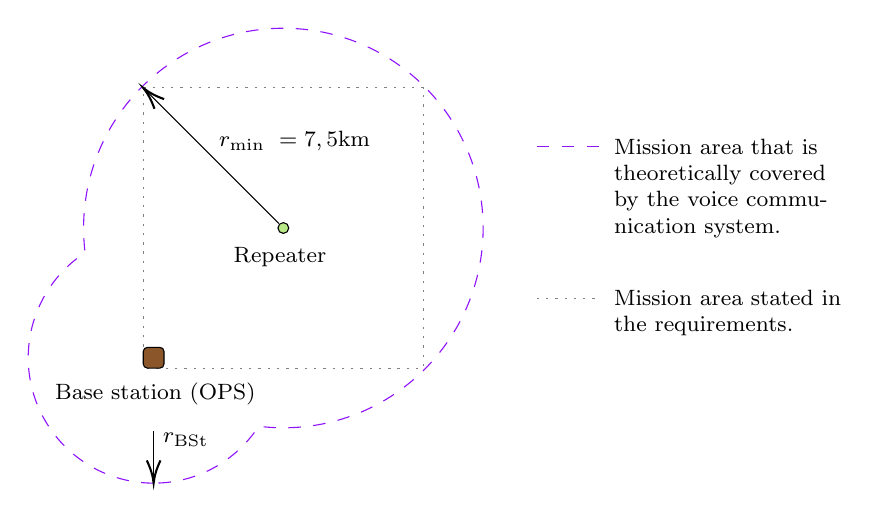
\begin{tikzpicture}[x=0.75pt,y=0.75pt,yscale=-1,xscale=1]
%uncomment if require: \path (0,409); %set diagram left start at 0, and has height of 409

%Shape: Rectangle [id:dp12443341375434458] 
\draw  [color={rgb, 255:red, 128; green, 128; blue, 128 }  ,draw opacity=1 ][dash pattern={on 0.84pt off 2.51pt}] (105.42,168.75) -- (240.42,168.75) -- (240.42,303.75) -- (105.42,303.75) -- cycle ;
%Shape: Path Data [id:dp8368288281183056] 
\draw  [color={rgb, 255:red, 144; green, 19; blue, 254 }  ,draw opacity=1 ][dash pattern={on 4.5pt off 4.5pt}] (110.42,359.17) .. controls (77.05,359.17) and (50,332.12) .. (50,298.75) .. controls (50,277.57) and (60.9,258.93) .. (77.4,248.14) .. controls (76.92,244.24) and (76.67,240.28) .. (76.67,236.25) .. controls (76.67,183.09) and (119.77,140) .. (172.92,140) .. controls (226.08,140) and (269.17,183.09) .. (269.17,236.25) .. controls (269.17,289.41) and (226.08,332.5) .. (172.92,332.5) .. controls (168.9,332.5) and (164.93,332.25) .. (161.04,331.77) .. controls (150.25,348.27) and (131.61,359.17) .. (110.42,359.17) -- cycle ;
%Rounded Rect [id:dp41901798669291956] 
\draw  [fill={rgb, 255:red, 139; green, 87; blue, 42 }  ,fill opacity=1 ] (105.42,295.75) .. controls (105.42,294.65) and (106.32,293.75) .. (107.42,293.75) -- (113.42,293.75) .. controls (114.53,293.75) and (115.42,294.65) .. (115.42,295.75) -- (115.42,301.75) .. controls (115.42,302.85) and (114.53,303.75) .. (113.42,303.75) -- (107.42,303.75) .. controls (106.32,303.75) and (105.42,302.85) .. (105.42,301.75) -- cycle ;
%Straight Lines [id:da8105217749265208] 
\draw    (110.42,357.17) -- (110.42,334.17) ;
\draw [shift={(110.42,359.17)}, rotate = 270] [color={rgb, 255:red, 0; green, 0; blue, 0 }  ][line width=0.75]    (10.93,-3.29) .. controls (6.95,-1.4) and (3.31,-0.3) .. (0,0) .. controls (3.31,0.3) and (6.95,1.4) .. (10.93,3.29)   ;
%Straight Lines [id:da3146532721436186] 
\draw    (106.84,170.16) -- (170.74,234.06) ;
\draw [shift={(105.42,168.75)}, rotate = 45] [color={rgb, 255:red, 0; green, 0; blue, 0 }  ][line width=0.75]    (10.93,-3.29) .. controls (6.95,-1.4) and (3.31,-0.3) .. (0,0) .. controls (3.31,0.3) and (6.95,1.4) .. (10.93,3.29)   ;
%Shape: Circle [id:dp5997567206989125] 
\draw  [fill={rgb, 255:red, 184; green, 233; blue, 134 }  ,fill opacity=1 ] (170.32,236.25) .. controls (170.32,234.81) and (171.49,233.65) .. (172.92,233.65) .. controls (174.36,233.65) and (175.52,234.81) .. (175.52,236.25) .. controls (175.52,237.69) and (174.36,238.85) .. (172.92,238.85) .. controls (171.49,238.85) and (170.32,237.69) .. (170.32,236.25) -- cycle ;
%Straight Lines [id:da1970463822196904] 
\draw [color={rgb, 255:red, 144; green, 19; blue, 254 }  ,draw opacity=1 ] [dash pattern={on 4.5pt off 4.5pt}]  (295,197) -- (325,197) ;

%Straight Lines [id:da2827334971957638] 
\draw [color={rgb, 255:red, 128; green, 128; blue, 128 }  ,draw opacity=1 ] [dash pattern={on 0.84pt off 2.51pt}]  (295,270) -- (325,270) ;


% Text Node
\draw (331,192) node [anchor=north west][inner sep=0.75pt]  [font=\footnotesize] [align=left] {Mission area that is \\theoretically covered\\by the voice commu-\\nication system. };
% Text Node
\draw (61.74,309.44) node [anchor=north west][inner sep=0.75pt]  [font=\footnotesize] [align=left] {Base station (OPS)};
% Text Node
\draw (147.74,244.44) node [anchor=north west][inner sep=0.75pt]  [font=\footnotesize] [align=left] {Repeater};
% Text Node
\draw (113.74,333.84) node [anchor=north west][inner sep=0.75pt]  [font=\footnotesize]  {$r_{\mathrm{BSt}}$};
% Text Node
\draw (140.74,188.46) node [anchor=north west][inner sep=0.75pt]  [font=\footnotesize]  {$r_{\mathrm{min}} \ =7,5\mathrm{km}$};
% Text Node
\draw (331,265) node [anchor=north west][inner sep=0.75pt]  [font=\footnotesize] [align=left] {Mission area stated in\\the requirements.};


\end{tikzpicture}

	\caption{Top view of the mission area covered by the voice communication system.}
	\label{fig:tikz_range}
\end{figure}
Figure \ref{fig:tikz_range} shows the top view of the mission area that is theoretically covered by the voice communication system \cite{Lange:1992}. The border of the mission area covered is illustrated with the dashed purple line. In it, the brown rounded square represents the base station, the green dot represents the repeater and the gray dotted square represents the mission area specified by the system requiremnts. According to these requiremnts the minimum radius is $r_\mathrm{min} = 7,5\mathrm{km}$, as a total mission area of approximately $10\mathrm{km}$ by $10\mathrm{km}$ has to be covered. Furthermore, the system was designed in such a way that the requiremnts are met for the least powerful radio device. 

Since the base station, like the repeater, uses an omnidirectional antenna, the participants of the voice communication system also have reception in an area with a radius $r_\mathrm{BSt}$ in $\left(\mathrm{m}\right)$ around it. By transforming the equation (\ref{eq:plane_earth_approx_db}) and assuming that the fade margin of the least powerful radio device stays the same for the entire coverage area, $r_\mathrm{BSt}$  can be calculated.\footnote{In the equation (\ref{eq:plane_earth_approx_db}), $r_\mathrm{BSt}$ corresponds to the distance $d$.} Although this extends the mission area, it must be taken into account that it may interfere with a neighboring radio system.

In the following subsections each part of the voice communication system will be introduced.

\subsection{Base station radio infrastructure}
The task of the base station crew is to monitor and coordinate both an ongoing mission and the on-site support crew. It is thus the central link of the voice communication system. The base station radio infrastructure is supplied by electrical energy from the local power grid and it consists of a Motorola Mototrbo DM 2600 mobile radio, a Diawa CN-501VN cross needle VSWR \& power meter to monitor the VSWR of the antenna feed line and detect possible errors, a Diamond SP1000 lightning arrester to protect the base station crew, the DM 2600 and the CN-501VN from the consequences of a lightning strike\footnote{It is not recommended to use the voice communication system in situations where lightning strikes may occur.} and a Diamond BC-101 VHF fixed station antenna. Besides that, several adapters and coaxial cables with different lengths $l$ in $\left(\mathrm{m}\right)$ are used to connect these devices and components with each other. 
\begin{figure}[h!]
	\centering
	\input{tikz/tikz_base_camp_radio}
	\caption{Schematic structure of the base station radio infrastructure.}
	\label{fig:tikz_base_camp_radio}
\end{figure}
Figure \ref{fig:tikz_base_camp_radio} provides an illustration. There are gaps between the devices and components to make the schematic structure easier to read.\footnote{In practice these are connected.} Green connectors represent a BNC plug or socket, turquoise connectors represent a PL plug or socket and pink connectors represent a N plug or socket. For more information on whether it is a socket or a plug, see figure \ref{fig:tikz_base_camp_radio} and tables \ref{tab:table_dm2600_specs} through \ref{tab:table_ultraflex_7_specs}. Adapters -- such as \circled{\footnotesize{1}} and \circled{\footnotesize{3}} -- are characterized by a rectangle with a diagonal drawn in. The colors in the resulting right-angled triangles indicate which connectors an adapter has. Coaxial cables are drawn with a thicker line and trapezoids as connectors -- for example \circled{\footnotesize{2}}, \circled{\footnotesize{5}} and \circled{\footnotesize{6}}. Because the coaxial cables were delivered without connectors, they were installed afterwards. The connectors of the DM 2600, Diawa CN-501VN, Diamond SP1000 and Diamond BC-101 are marked by a small rectangle which is in direct contact with the associated device or component. These have factory-installed connectors which their data sheets already take into account.

From the data sheet of the DM 2600, from which an excerpt is provided in table \ref{tab:table_dm2600_specs}, it can be seen that its maximum transmission power is $25\mathrm{W}$ and its sensitivity -- in the worst case -- is $0,25\mathrm{\mu V}$.
\begin{table}[h!]
	\centering
	\input{tables/table_dm2600_specs}
	\caption{Excerpt from the data sheet of the Motorola Mototrbo DM 2600 mobile radio. \cite{DM2600:2013}}
	\label{tab:table_dm2600_specs}
\end{table}
Its maximum transmission and minimum required reception power therefore follow to:
\begin{equation} \label{eq:power_BSt_tx}
	\centering
	P_\mathrm{T,dBW} =  10\mathrm{dBW} \cdot \log_{10} \left( \dfrac{25\mathrm{W}}{1\mathrm{W}} \right) = 13,979\mathrm{dBW}\text{,}
\end{equation}
\begin{equation} \label{eq:power_BSt_min}
	\centering
	P_\mathrm{min,dBW} = 10\mathrm{dBW} \cdot \log_{10} \left( \dfrac{\left(0,25\cdot10^{-6}\mathrm{V}\right)^2}{50\Omega} \right) = -149,031\mathrm{dBW}\text{.}
\end{equation}

It is assumed that the CN-501VN will not cause any loss or gain in the antenna feed line as its data sheet does not contain any specifications on this matter. An excerpt of said data sheet can be seen in the table \ref{tab:table_daiwa_cn_501}.
\begin{table}[h!]
	\centering
	\input{tables/table_daiwa_cn_501}
	\caption{Excerpt from the data sheet of the Daiwa CN-501VN cross needle VSWR \& power meter.\cite{Daiwa-industry-co.:2016}}
	\label{tab:table_daiwa_cn_501}
\end{table}

The SP1000 has an insertion loss of less than $0,2\mathrm{dB}$ and a VSWR of less than $1,2$ as shown in the table \ref{tab:table_lightning_arrestor_specs}.
\begin{table}[h!]
	\centering
	\input{tables/table_lightning_arrestor_specs}
	\caption{Excerpt from the data sheet of the Diamond SP1000 lightning arrester. \cite{SP1000:2020}}
	\label{tab:table_lightning_arrestor_specs}
\end{table}
If now the worst case is assumed -- which means that the insertion loss is exactly $0,2\mathrm{dB}$ and the VSWR is exactly $1,2$ -- then the total loss caused by this component is the sum of the insertion and the mismatch loss:
\begin{equation} \label{eq:losses_BSt_arr}
	\centering
	L_\mathrm{arr,dB} = 0,2\mathrm{dB} - 10\mathrm{dB} \cdot \log_{10} \left(1 - \left(\dfrac{1,2 - 1}{1,2 + 1}\right)^2\right) = 0,236\mathrm{dB}\text{.}
\end{equation}

As can be seen in the table \ref{tab:table_bc101_specs}, the BC-101 has a gain of $G_\mathrm{ant,dBi} = 3,5\mathrm{dBi}$ and a VSWR of less than $1,5$.
\begin{table}[h!]
	\centering
	\input{tables/table_bc101_specs}
	\caption{Excerpt from the data sheet of the Diamond BC-101 VHF fixed station antenna.\cite{antenna:2020}}
	\label{tab:table_bc101_specs}
\end{table}
With $\mathrm{VSWR} = 1,5$, the mismatch loss in the worst case can be calculated as shown in the equation (\ref{eq:losses_BSt_ant}).
\begin{equation} \label{eq:losses_BSt_ant}
	\centering
	L_\mathrm{ant,dB} = - 10\mathrm{dB} \cdot \log_{10} \left(1 - \left(\dfrac{1,5 - 1}{1,5 + 1}\right)^2\right) = 0,177\mathrm{dB}
\end{equation}
Regarding this antenna, it should also be mentioned that a mast will be made available at the mission site. Therefore, the height of the mast can vary from mission to mission. An antenna, which is set up on a $1\mathrm{m}$ high tripod on a freight container in accordance with ISO 668, has approximately a height of $h _\mathrm{BSt} = 3,6\mathrm{m}$ above the ground. This height is used for the link budget estimation. 

All coaxial cables used for the voice communication system are Messi \& Paoloni Ultraflex 7 coaxial cables. An excerpt of the data sheet of this coaxial cable can be found in the table \ref{tab:table_ultraflex_7_specs} and the attenuation as a function of the frequency -- interpolated with a \MATLAB program -- according to its data sheet, in the figure \ref{fig:image_attenuation_UF7}. 
\begin{table}[h!]
	\centering
	\input{tables/table_ultraflex_7_specs}
	\caption{Excerpt from the data sheet of the Messi \& Poloni Ultraflex 7 coaxial cable. \cite{Paoloni:2021}}
	\label{tab:table_ultraflex_7_specs}
\end{table}
\begin{figure}[h!]
	\centering
  	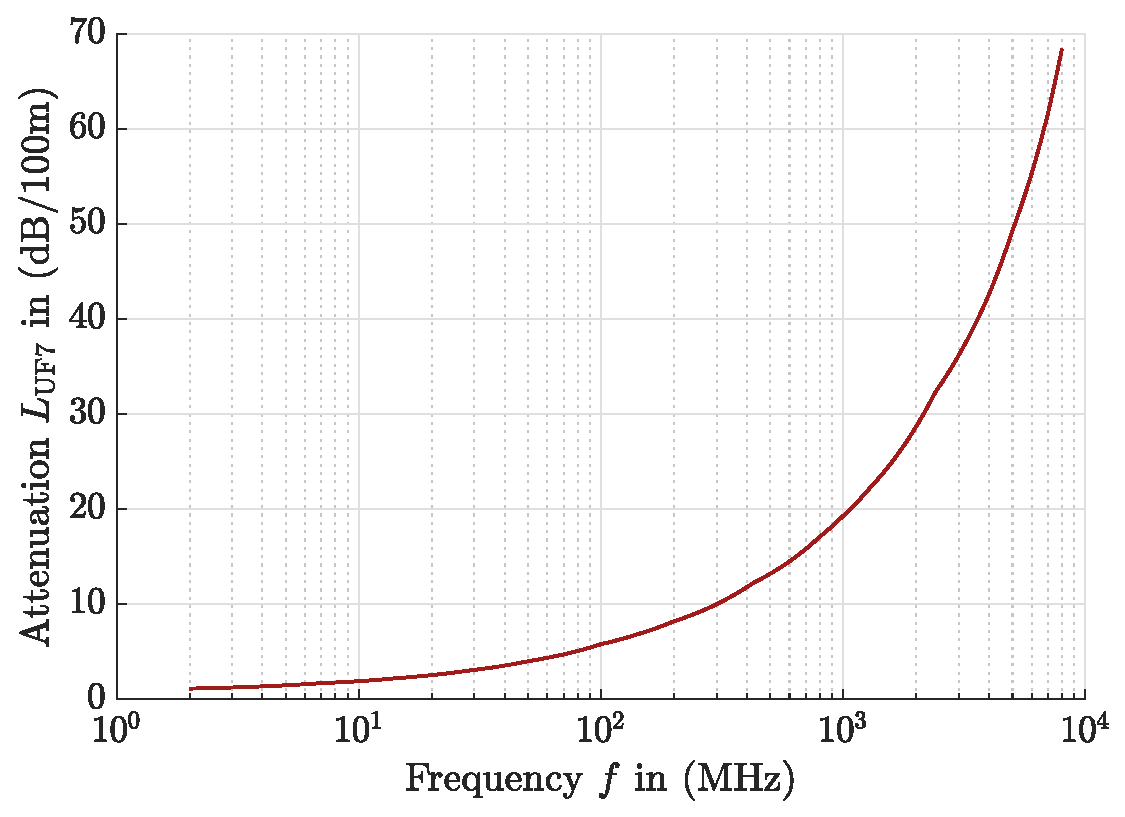
\includegraphics[width = 0.67\textwidth]{image_attenuation_UF7.eps}
  	\caption{Attenuation of the Messi \& Paoloni Ultraflex 7 coaxial cable for $20^\circ \mathrm{C}$. For the frequency $f_\sim = 158,950\mathrm{MHz}$, the attenuation is around $7,2471\mathrm{dB/100m}$. (Recreated from: \cite{Paoloni:2021})}
	\label{fig:image_attenuation_UF7}
\end{figure}
Based on this, an attenuation of $7,2471\mathrm{dB/100m}$ was determined for the frequency $f_\sim = 158,950\mathrm{MHz}$. The cable lengths of the individual coaxial cables in the systems can be taken from the figure \ref{fig:tikz_base_camp_radio}. This results in an insertion loss -- without connectors -- of:
\begin{equation} \label{eq:losses_BSt_coax}
	\centering
	L_\mathrm{coax,dB} = \dfrac{7,2471 \cdot 9,3}{100}\mathrm{dB} = 0,674\mathrm{dB}\text{.}
\end{equation}
It is noted, that $L_\mathrm{coax,dB}$ increases as the cable length increases. It can become significantly greater if the antenna is mounted at a location further away from the base station. 

Regarding the attenuation of the numbered adapters and connectors, which also includes the connectors of the coaxial cables in the figure \ref{fig:tikz_base_camp_radio}, it is assumed that each of these has an attenuation of $0,1 \mathrm{dB}$ \cite{LinkMargin:2016}. With $N_\mathrm{I} = 9$, the total insertion loss caused by the connectors and adapters follows to:
\begin{equation} \label{eq:losses_BSt_conn}
	\centering
	L_\mathrm{conn/adapt,dB} = 0,9\mathrm{dB}\text{.}
\end{equation}
An assumption was made because no data sheets for the adapters and connectors were found. 

From the above, the total loss of the antenna feed line now results in:
\begin{equation} \label{eq:losses_BSt}
	\centering
	L_\mathrm{BSt,dB} = L_\mathrm{arr,dB} + L_\mathrm{ant,dB} + L_\mathrm{coax,dB} + L_\mathrm{conn/adapt,dB} = 1,987\mathrm{dB}\text{.}
\end{equation}








%\textcolor{rgb, 255:red, 80; green, 227; blue, 194 }{turquoise} 




\subsection{Repeater radio infrastructure}
The main task of the repeater is to receive weak signals and to re-transmit them with increased transmission power. Its radio infrastructure is supplied by electrical energy from the self-sufficient energy distribution system, for which the schematic structure is shown in the figure \ref{fig:tikz_rep_energy}. As it can be seen, an AE Solar AE195SMM6-36 PV generator with pre-mounted cables \circled{\footnotesize{A}}, a Victron BlueSolar MPPT 75/10 SCC and an Offgridtec Smart-Pro $12,8\mathrm{V}$ $50\mathrm{Ah}$ $\mathrm{LiFePO}_4$ battery are used. In addition, the cables \circled{\footnotesize{B}} and \circled{\footnotesize{C}}, which are designed for harsh environments, are used to connect these devices.
\begin{figure}[h!]
	\centering
	\input{tikz/tikz_rep_energy}
	\caption{Schematic structure of the self-sufficient energy distribution system of the repeater radio infrastructure.}
	\label{fig:tikz_rep_energy}
\end{figure}
The SCC and the $\mathrm{LiFePO}_4$ battery are contained in an IP67 certified battery box to protect them from the environment. This IP rating also applies to the connectors in the small green rectangles. 

In the figure \ref{fig:tikz_rep_energy}, only the part necessary for the simulation of the self-sufficient energy distribution system can be seen. In practice, fuses, switches, lightning protection and other important components are also installed. Due to the short length of the cable that connects the $\mathrm{LiFePO}_4$ battery with the SCC, it was neglected. The simulation results of the self-sufficient energy distribution system of the repeater radio infrastructure can be found in the section \ref{sec:energy}. 

Continuing from the SLR 1000, the repeater radio infrastructure further consists of a Diamond SP1000 lightning arrester to protect the SLR 1000 and the self-sufficient energy distribution system from the consequences of a lightning strike and a Diamond BC-101 VHF fixed station antenna. As shown in the figure \ref{fig:tikz_repeater}, additional adapters, connectors and a coaxial cable are required. The adapter \circled{\footnotesize{1}} represents a $90^\circ$ angle.
\begin{figure}[h!]
	\centering
	\input{tikz/tikz_repeater}
	\caption{Schematic structure of repeater radio infrastructure.}
	\label{fig:tikz_repeater}
\end{figure}

Using the specifications of the SLR 1000 listed in the table \ref{tab:table_slr1000_specs}, the maximum transmission power is calculated in the equation (\ref{eq:power_rep_tx}). The minimum required reception power for the worst case can be taken from the equation (\ref{eq:power_BSt_min}).
\begin{table}[h!] % SLR1000
	\centering
	\input{tables/table_slr1000_specs}
	\caption{Excerpt from the data sheet of the Motorola Mototrbo SLR 1000 repeater. \cite{SLR1000:2019}}
	\label{tab:table_slr1000_specs}
\end{table}
\begin{equation} \label{eq:power_rep_tx}
	\centering
	P_\mathrm{T,dBW} =  10\mathrm{dBW} \cdot \log_{10} \left( \dfrac{10\mathrm{W}}{1\mathrm{W}} \right) = 10\mathrm{dBW}\text{,}
\end{equation}

Since the repeater uses the same lightning arrester and the same antenna as the base station, the resulting losses can be taken directly from the equations (\ref{eq:losses_BSt_arr}) and (\ref{eq:losses_BSt_ant}). The antenna of the repeater is always mounted at a height of $h_\mathrm{REP} = 8\mathrm{m}$ above the ground, as a mast is included in the system design. 

As can be seen in the figure \ref{fig:tikz_repeater}, the length of the coaxial cable is $0,5\mathrm{m}$, resulting in an insertion loss of:   
\begin{equation} \label{eq:losses_BSt_coax}
	\centering
	L_\mathrm{coax,dB} = \dfrac{7,2471 \cdot 0,5}{100}\mathrm{dB} = 0,036\mathrm{dB}\text{.}
\end{equation}

With the number of adapters and connectors $N_\mathrm{I} = 4$, their insertion loss follows to:
\begin{equation} \label{eq:losses_rep_conn}
	\centering
	L_\mathrm{conn/adapt,dB} = 0,4\mathrm{dB}\text{.}
\end{equation}

Finally, the total loss of the antenna feed line can be calculated with:
\begin{equation} \label{eq:losses_rep}
	\centering
	L_\mathrm{REP,dB} = L_\mathrm{arr,dB} + L_\mathrm{ant,dB} + L_\mathrm{coax,dB} + L_\mathrm{conn/adapt,dB} = 0,849\mathrm{dB}\text{.}
\end{equation}

\subsection{Serenity radio system}
As mentioned earlier, Serenity is the spacesuit simulator that the AAs use to conduct analog Mars missions. Its radio system consists of a Motorola Mototrbo SL 2600 handheld radio with a Motorola PMAD4156A antenna, a \emph{push-to-talk} (PTT) button and a Jabra Storm Bluetooth headset. The antenna is attached directly to the handheld radio and the entire system is built into the spacesuit simulator with the upper part of the antenna sticking out. Since the SL 2600 radio supports Bluetooth 4.0, it was decided that communication with the headset should take place via Bluetooth. This has two advantages. Firstly, the AA can put on the headset before donning and thus simply step into the spacesuit simulator, and secondly, the amount of cabling is reduced. The PTT button is wired to the outside of the spacesuit so that the AA can press it to communicate. A schematic structure of this system is illustrated in the figure \ref{fig:tikz_serenity_radio_system}.
\begin{figure}[h!]
	\centering
	\input{tikz/tikz_serenity_radio_system}
	\caption{Schematic structure of the Serenity radio system.}
	\label{fig:tikz_serenity_radio_system}
\end{figure}

Electrical energy is provided to the SL 2600 via its $2,3\mathrm{Ah}$ lithium-ion battery (Motorola PMNN4468B) which is charged with the electrical energy from the local power grid between missions. At a later point in time, the radio system can be upgraded in such a way, that the SL 2600 can be directly charged from the spacesuit simulator. Similar to the SL 2600, the Bluetooth headset is also supplied with electrical energy from its battery, but can only be charged via the local power grid. 

The maximum transmission power of the SL 2600, as shown in the equation (\ref{eq:power_SER_tx}), is calculated based on its specifications in the table \ref{tab:table_sl2600_specs}.
\begin{table}[h!] % SL2600
	\centering
	\input{tables/table_sl2600_specs}
	\caption{Excerpt from the data sheet of the Motorola Mototrbo SL 2600 handheld radio. \cite{SL2600:2017}}
	\label{tab:table_sl2600_specs}
\end{table}
\begin{equation} \label{eq:power_SER_tx}
	\centering
	P_\mathrm{T,dBW} =  10\mathrm{dBW} \cdot \log_{10} \left( \dfrac{3\mathrm{W}}{1\mathrm{W}} \right) = 4,771\mathrm{dBW}\text{,}
\end{equation}
As with the SLR 1000, the minimum required reception power for the worst case can be taken from the equation (\ref{eq:power_BSt_min}). At this point, the assumption is made that the antenna impedance is $50\Omega$, as no further specifications could be found. It was furthermore assumed that there are no losses in the antenna feed line and that the antenna has a gain of $0\mathrm{dBi}$. 


In cooperation with the Serenity \emph{structures} (STRUC) team, a position for the SL 2600 in the HUT of the spacesuit simulator was found, so that its antenna is upright at a height of $1,65\mathrm{m}$ above the ground for a standard male AA, or at a height of $1,55\mathrm{m}$ above the ground for a standard female AA \cite{Hinker:2007}. Regarding the link budget estimation $h_\mathrm{SER} = 1,55\mathrm{m}$ is used. In its installed position the device can be recharged and, if necessary, removed for maintenance purposes. This fulfills the requirement that the Serenity radio system must fit into the HUT. 

Taking into account the requirements for the operating temperature of the radio system, the data sheets of the SL 2600 (see table \ref{tab:table_sl2600_specs}) and the PTT button, including the wires and connectors involved, show that these are met. Due to the large push area of the PTT button, it was adopted from the Aouda spacesuit simulator, which is the predecessor of Serenity. No specifications were found for the Bluetooth headset and the audio jack that connects the PTT button to the SL 2600. The prototype still needs to be tested in this regard. However, if these do not meet the requirements, a suitable audio jack can be requested directly from Motorola Solutions Inc. and the Motorola EP900w Bluetooth headset can be procured \cite{push_switch:2011, EP900w:2021}.

The most important factor that needed to be considered when developing the radio system was its mass. As stated in the requirements, the combined mass of the W-LAN and VHF based communication systems must not exceed $1000\mathrm{g}$. At the time the Serenity (VHF) radio system was developed, the W-LAN based communication system had a mass of $605,33\mathrm{g}$. The total mass of the (VHF) radio system is $248\mathrm{g}$. This results in a combined mass of $853,33\mathrm{g}$. $9\mathrm{g}$ of this is the mass of the Jabra Storm Bluetooth headset. Should it be replaced by the Motorola EP900w Bluetooth headset, the (VHF) radio system would then have a mass of $261\mathrm{g}$, which results in a combined mass of $866,33\mathrm{g}$. The measurements were conducted with a digital kitchen scale from WMF (Model No.: 06.0873.6040). In the case that the audio jack needs to be changed, its mass is likely to remain the same. Since the W-LAN based communication system is not finished, it cannot be said at this point whether the mass requirement has
 been met. 


\subsection{Safety officer radio}
The safety officers do not interact directly with the AAs during an ongoing mission, but intervene in certain events. During these events it is crucial that voice communication is established between these two groups. For this purpose, the safety officers use a Motorola Mototrbo SL 2600 handheld radio with the same antenna and lithium-ion battery as that of the AAs. The battery of the SL 2600 is charged by the local power grid between missions.

The maximum transmission power is the same as in the equation (\ref{eq:power_SER_tx}) and the minimum required reception power for the worst case is the same as in the equation (\ref{eq:power_BSt_min}).

Regarding the antenna, the same assumptions are made as for the Serenity radio system. However, its height above the ground was determined based on the anthropometric dimensional data for an american female and male, shown in the figures \ref{fig:image_female} and \ref{fig:image_male}.
\begin{figure}[h!]
	\centering
	\begin{subfigure}[b]{0.3\textwidth}
		\centering
		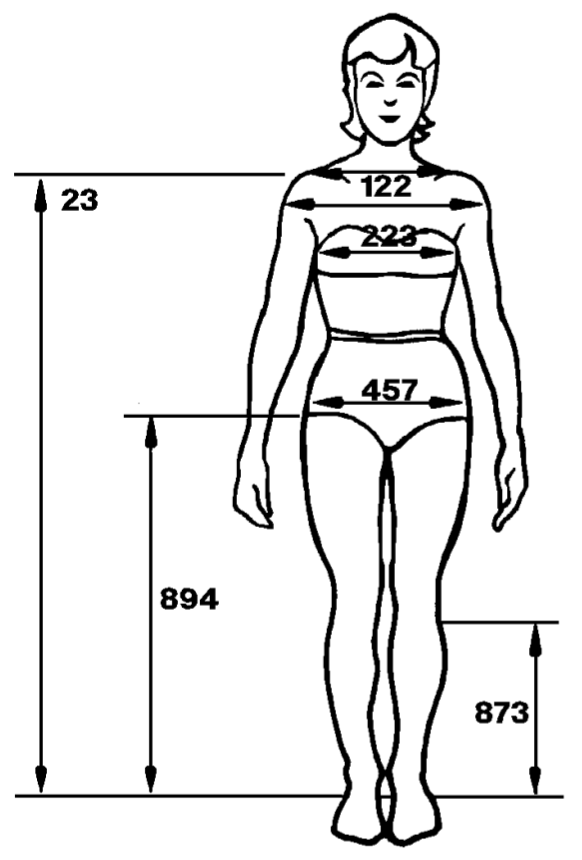
\includegraphics[width = \textwidth]{image_female}
		\caption{\textit{``Body Size of the 40-Year-Old Japanese Female for Year 2000 in One Gravity Conditions.''} \textbf{23} $\widehat{=}$ 1,271m.}
		\label{fig:image_female}
	\end{subfigure}
	\hspace{60pt}
	\begin{subfigure}[b]{0.3\textwidth}
		\centering
		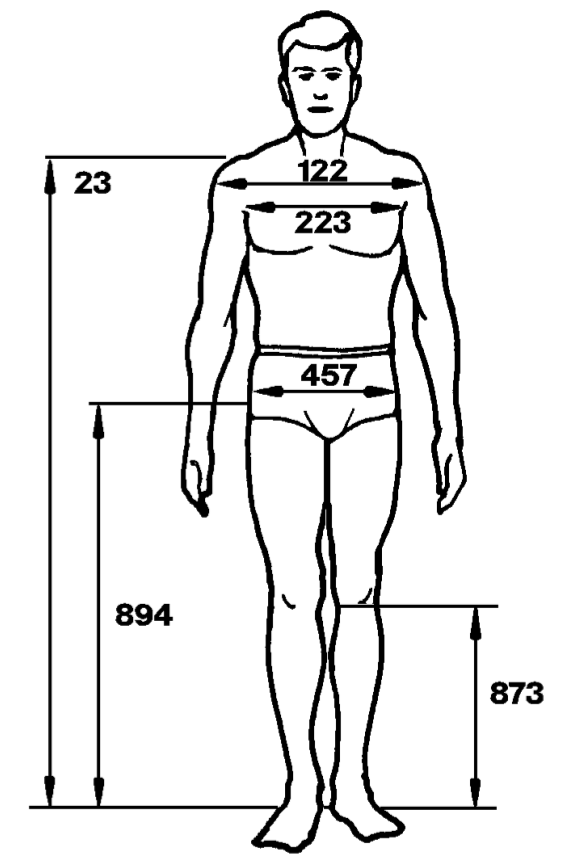
\includegraphics[width = \textwidth]{image_male}
		\caption{\textit{``Body Size of the 40-Year-Old American Male for Year 2000 in One Gravity Conditions.''} \textbf{23} $\widehat{=}$ 1,476m.}
		\label{fig:image_male}
	\end{subfigure}
	\caption{Anthropometric dimensional data for the american female and male. (Image and caption credit: \cite{Hinker:2007, Adolf:2020})}
	\label{fig:bodies}
\end{figure}
When it is assumed that the SL 2600 is operated at shoulder height, then its antenna is $1,271\mathrm{m}$ above the ground for a female and $1,476\mathrm{m}$ above the ground for a male safety officer \cite{Hinker:2007, Adolf:2020}. For the link budget estimation $h_\mathrm{SFTY} = 1,271\mathrm{m}$ is used.
\subsection{On-site support crew radio}
The on-site support crew, which carries out general tasks in the mission area, uses the DP 3601 handheld radios. These are supplied with electrical energy from their $2,15\mathrm{Ah}$ lithium-ion batteries (Motorola PMNN4103A) which are charged via the local power grid when required.  

According to the same principle as in the previous subsections, the maximum transmission power of the DP 3601 can be calculated using the equation (\ref{eq:power_OSS_tx}), with its specifications being listed in the table \ref{tab:table_dp3601_specs}.
\begin{table}[h!] % DP3601
	\centering
	\input{tables/table_dp3601_specs}
	\caption{Excerpt from the data sheet of the Motorola Mototrbo DP 3601 handheld radio. \cite{DP3601:2010}}
	\label{tab:table_dp3601_specs}
\end{table}
\begin{equation} \label{eq:power_OSS_tx}
	\centering
	P_\mathrm{T,dBW} =  10\mathrm{dBW} \cdot \log_{10} \left( \dfrac{5\mathrm{W}}{1\mathrm{W}} \right) = 6,99\mathrm{dBW}\text{,}
\end{equation}
Since the DP 3601 is an older handheld radio, its sensitivity differs from that of the other Motorola Mototrbo radio devices mentioned earlier. By assuming that the antenna impedance is $50\Omega$ -- due to the same reasons as for the SL 2600 -- the minimum required reception power follows to:
\begin{equation} \label{eq:power_OSS_min}
	\centering
	P_\mathrm{min,dBW} = 10\mathrm{dBW} \cdot \log_{10} \left( \dfrac{\left(0,30\cdot10^{-6}\mathrm{V}\right)^2}{50\Omega} \right) = -147,447\mathrm{dBW}\text{.}
\end{equation}

The antenna of the DP 3601 is directly attached to the radio and it is assumed, that no losses in the antenna feed line occur. Furthermore, its gain is assumed to be $0\mathrm{dBi}$ and, as in the previous subsection, its hight above the ground is assumed to be $h_\mathrm{OSS} = 1,271\mathrm{m}$.






\section{Link budget estimation}
In this section it is examined whether the range of the theoretically covered mission area is fulfilled according to the requirements. For this purpose, the link margins of the participants that can freely move and the base station, at a distance of $r_\mathrm{min}= 7,5\mathrm{km}$ from the repeater, are determined. If their margins are around $20\mathrm{dB}$ to $30\mathrm{dB}$, the range requirement for the case described in the subsection \ref{sec:pepl} is met. Regarding the Motorola Mototrbo radio devices, it can then be said that the BER within the theoretically covered mission area is less than $5\%$. After evaluating the results, the radio device -- from the group of participants that can freely move -- with the smallest fade margin is determined and the radius $r_\mathrm{BSt}$ is calculated.

Table \ref{tab:table_system_results} provides a summary of the designed voice communication system discussed in the previous section in relation to the link budget. For completness it is mentioned that $G_\mathrm{ant,dB}$ in $\left(\mathrm{dBi}\right)$ is the antenna gain, $L_\mathrm{tot,dB}$ in $\left(\mathrm{dB}\right)$ is the total loss of the antenna feed line and $h_\mathrm{ant}$ in $\left(\mathrm{dB}\right)$ is the antenna height above the ground, of a certain radio system.
\begin{table}[h!]
	\centering
	\footnotesize
\begin{tabular}{|c|c|c|c|c|c|}
	\hline
	\textbf{Radio system} & $\boldsymbol{\mathrm{EIRP}_\mathrm{dBW}}$ & $\boldsymbol{P_\mathrm{min,dBW}}$ & $ \boldsymbol{G_\mathrm{ant,dBi}} $  & $\boldsymbol{L_\mathrm{tot,dB}}$ & $\boldsymbol{h_\mathrm{ant}}$ \\
	\hline
	BSt & $17,479\mathrm{dBW}$ & $-149,031\mathrm{dBW}$ & $3,5\mathrm{dBi}$ &  $1,987\mathrm{dB}$ & $3,6\mathrm{m}$ \\
	REP & $13,5\mathrm{dBW}$ & $-149,031\mathrm{dBW}$ &  $3,5\mathrm{dBi}$ & $0,849\mathrm{dB}$ & $8\mathrm{m}$ \\
	SER & $4,771\mathrm{dBW}$ & $-149,031\mathrm{dBW}$ & $0\mathrm{dBi}$ & $0\mathrm{dB}$ & $1,55\mathrm{m}$ \\
	SFTY & $4,771\mathrm{dBW}$  &  $-149,031\mathrm{dBW}$ &  $0\mathrm{dBi}$ & $0\mathrm{dB}$ & $1,271\mathrm{m}$ \\
	OSS & $6,99\mathrm{dBW}$ & $-147,447\mathrm{dBW}$ &  $0\mathrm{dBi}$ & $0\mathrm{dB}$ & $1,271\mathrm{m}$ \\
	\hline
\end{tabular}
	\caption{Specifications of the designed voice communication system when all participants transmit at maximum power.}
	\label{tab:table_system_results}
\end{table}

Since the Austrian authorities have only permitted a maximum transmission power of $P_\mathrm{T} = 5\mathrm{W}$, the case in which this is the maximum transmission power of the base station and the repeater is also taken into account. Table \ref{tab:table_system_results_5w} summarizes this with the new $\mathrm{EIRP}_\mathrm{dBW}$ for these radio systems marked in orange. 
\begin{table}[h!]
	\centering
	\footnotesize
\begin{tabular}{|c|c|c|c|c|c|}
	\hline
	\textbf{Radio system} & $\boldsymbol{\mathrm{EIRP}_\mathrm{dBW}}$ & $\boldsymbol{P_\mathrm{min,dBW}}$ & $ \boldsymbol{G_\mathrm{ant,dBi}} $  & $\boldsymbol{L_\mathrm{tot,dB}}$ & $\boldsymbol{h_\mathrm{ant}}$ \\
	\hline
	BSt & $\color{rgb, 255:red, 196; green, 135; blue, 29 }10,49\mathrm{dBW}$ & $-149,031\mathrm{dBW}$ & $3,5\mathrm{dBi}$ & $1,987\mathrm{dB}$ & $3,6\mathrm{m}$ \\
	REP & $\color{rgb, 255:red, 196; green, 135; blue, 29 }10,49\mathrm{dBW}$ & $-149,031\mathrm{dBW}$ & $3,5\mathrm{dBi}$ & $0,849\mathrm{dB}$ & $8\mathrm{m}$ \\
	SER & $4,771\mathrm{dBW}$ & $-149,031\mathrm{dBW}$ & $0\mathrm{dBi}$ & $0\mathrm{dB}$ & $1,55\mathrm{m}$ \\
	SFTY & $4,771\mathrm{dBW}$  &  $-149,031\mathrm{dBW}$ & $0\mathrm{dBi}$ & $0\mathrm{dB}$ & $1,271\mathrm{m}$ \\
	OSS & $6,99\mathrm{dBW}$ & $-147,447\mathrm{dBW}$ & $0\mathrm{dBi}$ & $0\mathrm{dB}$ & $1,271\mathrm{m}$ \\
	\hline
\end{tabular}
	\caption{Specifications of the designed voice communication system when all participants are limited to a maximum transmission power of $P_\mathrm{T} = 5\mathrm{W}$.}
	\label{tab:table_system_results_5w}
\end{table}

\subsection{Communication links and fade margin} \label{sec:comm_link_fade_margin}
If the radio system parameters in the table \ref{tab:table_system_results} -- for maximum transmission power -- and the distance $d \ \widehat{=} \ r_\mathrm{min} = 7,5\mathrm{km}$ are now used in the equation (\ref{eq:plane_earth_approx_db}), the results in the table \ref{tab:table_link_margin_max} are obtained.
\begin{table}[h!]
	\centering
	\input{tables/table_link_margin_max}
	\caption{Results of the plane earth signal budget calculation for the designed voice communication system when all participants transmit at maximum power.}
	\label{tab:table_link_margin_max}
\end{table}
The arrows in the column called \textbf{Link} represent the communcation direction.

In the same way the results in the table \ref{tab:table_link_margin_5w} are obtained. However, these apply when the voice communication system is limited to a maximum transmission power of $P_\mathrm{T} = 5\mathrm{W}$. Those radio links on which this has an effect are marked in orange. 
\begin{table}[h!]
	\centering
	\input{tables/table_link_margin_5w}
	\caption{Results of the plane earth signal budget calculation for the designed voice communication system when all participants are limited to a maximum transmission power of $P_\mathrm{T} = 5\mathrm{W}$.}
	\label{tab:table_link_margin_5w}
\end{table}

From both tables it can be seen that the link margins marked in green are above $20\mathrm{dB}$. The lowest link margin is $21,595\mathrm{dB}$ and it occurs when a safety officer is $7,5\mathrm{km}$ away from the repeater and communicates through it.

Due to the fact that the plane earth model is used, these calculations are only estimations. In order to study the performance of the designed voice communication system in more detail, experiments must be carried out on it in order to obtain empirical data. 

In theory, the safety officers and AAs, with each group being located somewhere within a distnace of $r_\mathrm{min} = 7,5\mathrm{km}$ around the repeater, can communicate -- via said repeater -- with each other. In practice, however, it is important that both groups maintain LOS either to the repeater or to each other and that the OeWF uses the topology of the mission area to the advantage of the designed voice communication system. If there are elevations in the mission area, then these should preferably be used as installation sites of the base station and the repeater. This increases their antenna heights and thus their fade margins. Depending on the topology of the mission area, the LOS can be maintained more easily with antennas being mounted at higher locations. If LOS cannot be maintained due to the topology of the mission area, this compromise must be made, and if necessary, the mission planning must be adapted to it. 
\subsection{Additional coverage area around the base station}
As shown in the figure \ref{fig:tikz_range}, the participants of the designed voice communication system that can freely move also receive a transmitted signal from the base station at a distance $r_\mathrm{BSt}$ around it. So that the link margin of $21,595\mathrm{dB}$ for the least powerfull radio device is constant in the entire system, the distance $r_\mathrm{BSt}$ follows from transforming the equation (\ref{eq:plane_earth_approx_db}) to: 
\begin{equation} \label{eq:r_bst}
	\centering
	\begin{aligned}
	r_\mathrm{BSt} &= \sqrt{\dfrac{1,271 \cdot 3,6 \mathrm{m}^2}{10^{\left(\dfrac{-127,436\mathrm{dBW} - 4,771\mathrm{dBW} - 3,5\mathrm{dBi} + 1,987\mathrm{dB}}{20\mathrm{dB}}\right)}}} \\ 
	&= 4712,20\mathrm{m}\text{.}
	\end{aligned}
\end{equation}
In this case there is no need to differentiate between the maximum transmission power and the transmission power limited to $5\mathrm{W}$ of the base station, since the $3\mathrm{W}$ transmission power of the safety officer's radio is the decisive factor. 

Since the repeater may not receive the signal from the safety officers and the AAs in this area, it is necessary to calculate the maximum distance that the safety officers can take to the AAs. It is calculated in the same manner as the equation (\ref{eq:r_bst}) and results in:
\begin{equation} \label{eq:r_ser_sfty}
	\centering
	r_\mathrm{SER,SFTY} = \sqrt{\dfrac{1,271 \cdot 1,55 \mathrm{m}^2}{10^{\left(\dfrac{-127,436\mathrm{dBW} - 4,771\mathrm{dBW}}{20\mathrm{dB}}\right)}}} = 2834,09\mathrm{m}\text{.}
\end{equation}

The distances calculated in the equations (\ref{eq:r_bst}) and (\ref{eq:r_ser_sfty}) may appear large, but what has already been mentioned in the section \ref{sec:comm_link_fade_margin} must be taken into account. 


 
 
\section{Self-sufficient energy distribution system} \label{sec:energy}
Now the self-suficient energy distribution system of the repeater radio infrastructure is being examined. For this purpose, the PV generators used are first introduced and their behavior for different values of the PV cell temperature $\vartheta_\mathrm{C}$ and the solar irradiance $E_\mathrm{G}$ is examined based on the model mentioned in the subsection \ref{sec:photovoltaic_generators}. The $\mathrm{LiFePO}_4$ battery used is then introduced and the results from the experiments discussed in the subsection \ref{sec:electrochemical} are presented. Finally, the remaining components required for the self-sufficient energy distribution system are introduced and a performance estimation based on a \MATLAB simulation (see appendix \ref{sec:matlab_code}) is carried out in order to assess whether it can supply the repeater radio infrastructure with electrical energy. 

\subsection{Photovoltaic generator model} \label{sec:pv_gen_mod}
In general, two different PV generators are examined. Namely the AE Solar AE195SMM6-36 and the DAS Energy DAS145PF. Only one (primary) PV generator is used to suppliy the repeater radio infrastructure with electrical energy, with the second one serving as a backup. The backup PV generator is installed when the primary one fails to convert the required amount of electrical energy. This is the case, for example, if it gets damaged during an ongoing mission. Since both PV generators have a similar power output $P_\mathrm{PV}$, it is up to the OeWF to decide which one is used as the primary and which one as the backup. Excerpts from their data sheets can be found in the tables \ref{tab:table_ae_solar_pvg_specs} and \ref{tab:table_das_energy_pvg_specs}.
\begin{table}[h!]
	\centering
	\input{tables/table_ae_solar_pvg_specs}
	\caption{Excerpt from the data sheet of the AE Solar AE195SMM6-36 PV generator at STC \cite{ae_solar:2019}.}
	\label{tab:table_ae_solar_pvg_specs}
\end{table}
\begin{table}[h!]
	\centering
	\input{tables/table_das_energy_pvg_specs}
	\caption{Excerpt from the data sheet of the DAS Energy DAS145PF PV generator at STC \cite{das_energy_2017}.}
	\label{tab:table_das_energy_pvg_specs}
\end{table}

As can be seen from the results of the \MAPLE source code in the appendix \ref{sec:maple_code}, it makes little difference for the first few decimal places if the model is approximated with the Jacobian matrix. In the \MAPLE source code, the caluclations are performed for the AE Solar AE195SMM6-36 PV generator, with its PV cell temperature being $\vartheta_\mathrm{C} = 25^\circ\mathrm{C}$ and the total irradiance onto its inclined surface being $E_\mathrm{G} = 200\mathrm{Wm}^{-2}$. These results can be replicated for the DAS Energy DAS145PF PV generator and for other values of $\vartheta_\mathrm{C}$ and $E_\mathrm{G}$ as well. Therefore, it can be said that the starting values shown in the equation (\ref{eq:U_OC_I_S_zero}) suffice as a good approximation for the PV generator's open-circuit voltage $U_\mathrm{OC}$ and reverse saturation current $I_\mathrm{S}$. This is because $I_\mathrm{S}$ is usually very small \cite{Mertens:2015, Wagner:2018}. 

The results for the modeled current-voltage and power-voltage characteristics of the AE Solar AE195SMM6-36 PV generator, depending on either the total irradiance onto its inclined surface $E_\mathrm{G}$ or on its PV cell temperature $\vartheta_\mathrm{C}$, can be seen in the figures \ref{fig:image_curr_volt_irr_ae_solar}, \ref{fig:image_power_volt_irr_ae_solar}, \ref{fig:image_curr_volt_temp_ae_solar} and \ref{fig:image_power_volt_temp_ae_solar}. If it depends on $E_\mathrm{G}$ it is assumed that $\vartheta_\mathrm{C} = 25^\circ\mathrm{C}$ is constant, and if it depends on $\vartheta_\mathrm{C}$ it is assumed that $E_\mathrm{G} = 1000\mathrm{Wm}^{-2}$ is constant. These constant vlaues for $\vartheta_\mathrm{C}$ and $E_\mathrm{G}$ were chosen because they represent the STCs. Identically, the results for the DAS Energy DAS145PF PV generator can be taken from the figures \ref{fig:image_curr_volt_irr_das_energy}, \ref{fig:image_power_volt_irr_das_energy}, \ref{fig:image_curr_volt_temp_das_energy} and \ref{fig:image_power_volt_temp_das_energy}. All results were obtained by programming the discussed model of a PV generator in \MATLAB.

From the current-voltage characteristics for different irradiance levels $E_\mathrm{G}$ of both PV generators shown in the figures \ref{fig:image_curr_volt_irr_ae_solar} and \ref{fig:image_curr_volt_irr_das_energy}, it can be seen that the short-circuit current $I_\mathrm{SC}$ decreases faster than the open-circuit voltage $U_\mathrm{OC}$. This is due to the fact that $I_\mathrm{Ph} = I_\mathrm{SC}$ is proportional to $E_\mathrm{G}$ (compare to equation (\ref{eq:i_ph_theta_phi})), while $U_\mathrm{OC}$ changes with the natural logarithm to it (compare to equations (\ref{eq:U_OC_theta_phi}) and \ref{eq:U_OC_I_S_zero})) \cite{Mertens:2015}.
\begin{figure}[h!]
	\centering
  	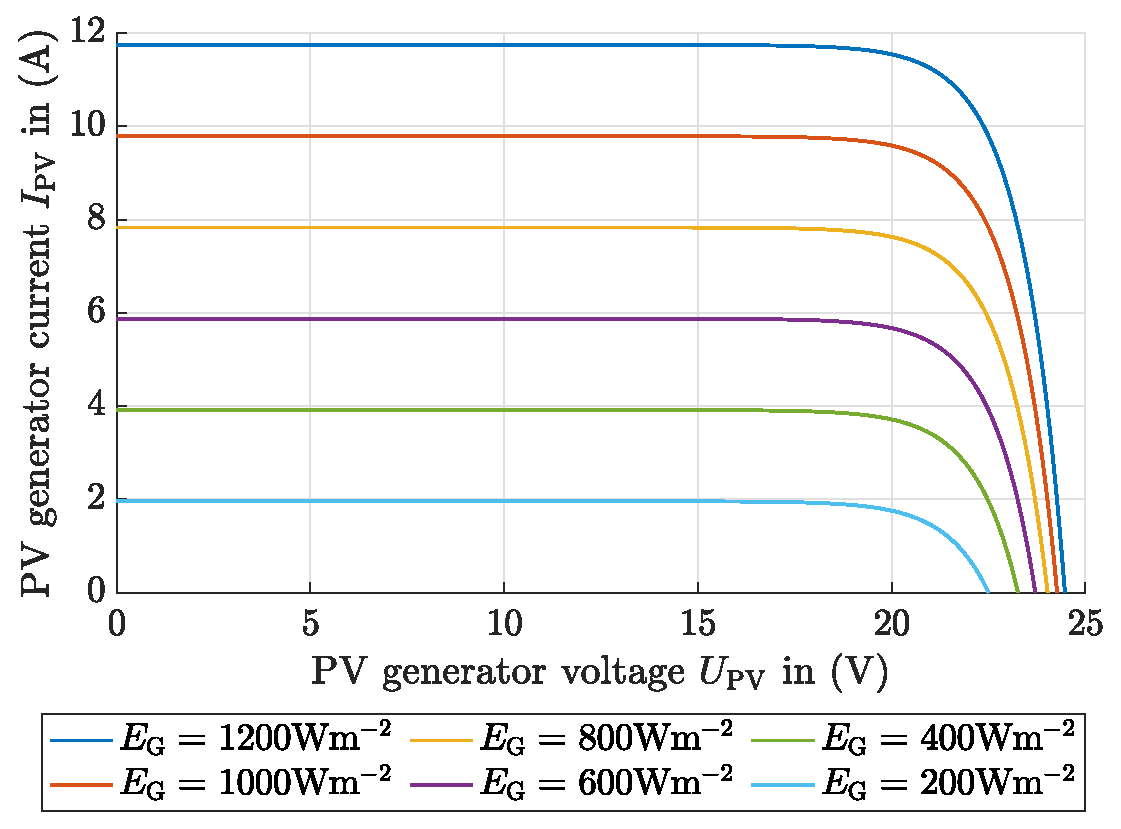
\includegraphics[width = 0.67\textwidth]{image_curr_volt_irr_ae_solar.eps}
  	\caption{Modeled current-voltage characteristic of the AE Solar AE195SMM6-36 PV generator, depending on the total irradiance onto its inclined surface $E_\mathrm{G}$. The PV cell temperature $\vartheta_\mathrm{C} = 25^\circ\mathrm{C}$ is assumed to be constant.}
	\label{fig:image_curr_volt_irr_ae_solar}
\end{figure}
\begin{figure}[h!]
	\centering
  	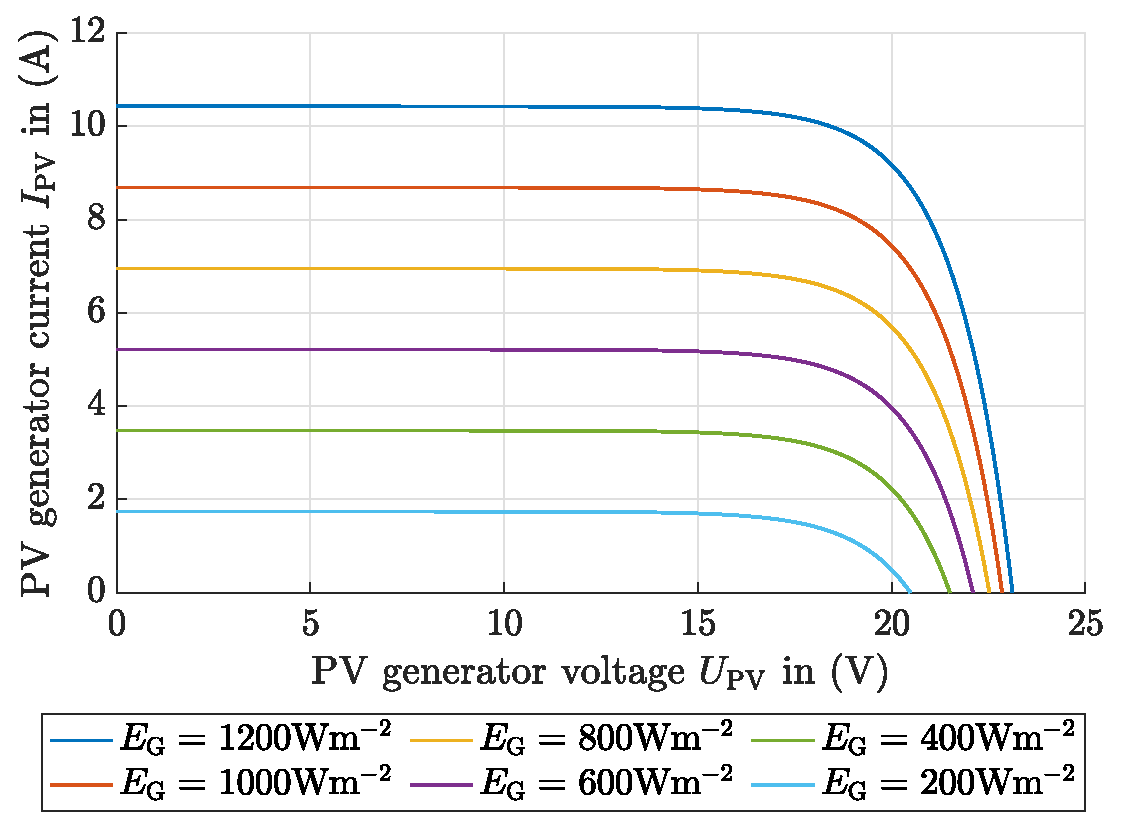
\includegraphics[width = 0.67\textwidth]{image_curr_volt_irr_das_energy.eps}
  	\caption{Modeled current-voltage characteristic of the DAS Energy DAS145PF PV generator, depending on the total irradiance onto its inclined surface $E_\mathrm{G}$. The PV cell temperature $\vartheta_\mathrm{C} = 25^\circ\mathrm{C}$ is assumed to be constant.}
	\label{fig:image_curr_volt_irr_das_energy}
\end{figure}

Now the associated power-voltage characteristics for different irradiance levels $E_\mathrm{G}$ of both PV generators can be calculated by using the equation (\ref{eq:p_pv_u}), as shown in the figures \ref{fig:image_power_volt_irr_ae_solar} and \ref{fig:image_power_volt_irr_das_energy}. As can be observed from a real PV generator, the power output $P_\mathrm{PV}$ decreases with lower irradiance levels $E_\mathrm{G}$. 
\begin{figure}[h!]
	\centering
  	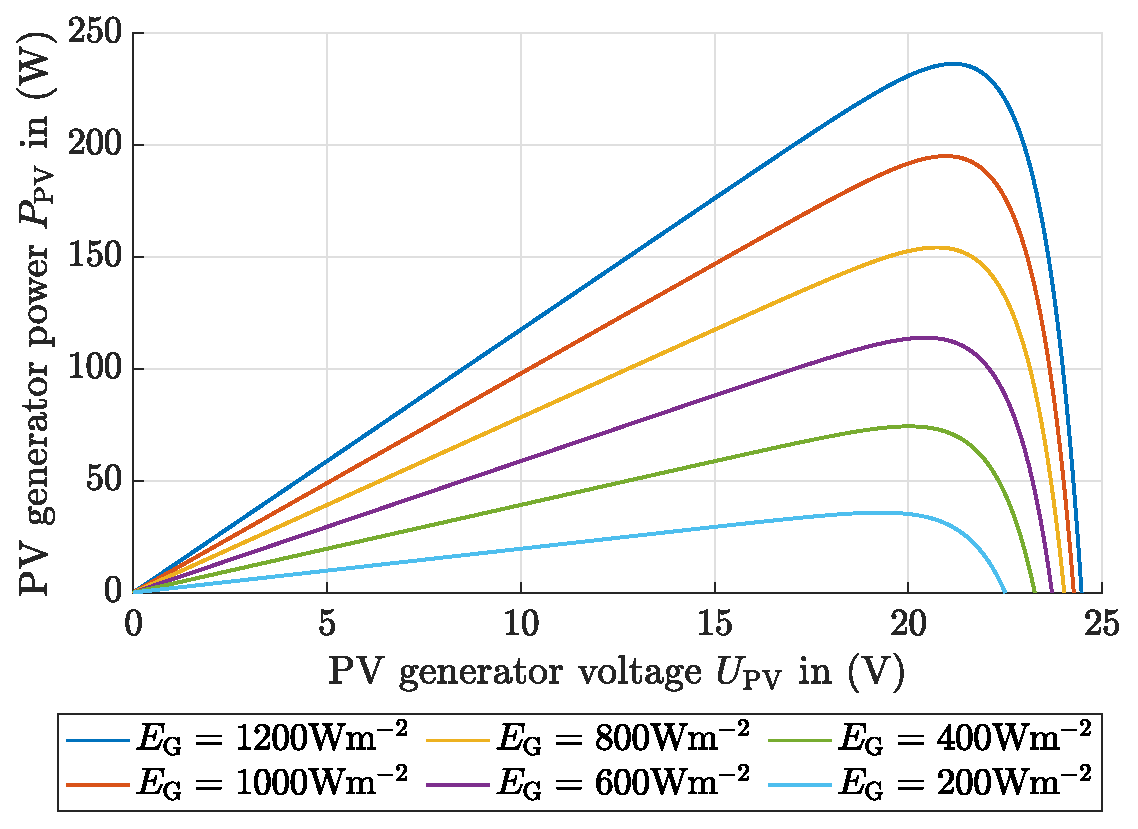
\includegraphics[width = 0.67\textwidth]{image_power_volt_irr_ae_solar.eps}
  	\caption{Modeled power-voltage characteristic of the AE Solar AE195SMM6-36 PV generator, depending on the total irradiance onto its inclined surface $E_\mathrm{G}$. The PV cell temperature $\vartheta_\mathrm{C} = 25^\circ\mathrm{C}$ is assumed to be constant.}
	\label{fig:image_power_volt_irr_ae_solar}
\end{figure}
\begin{figure}[h!]
	\centering
  	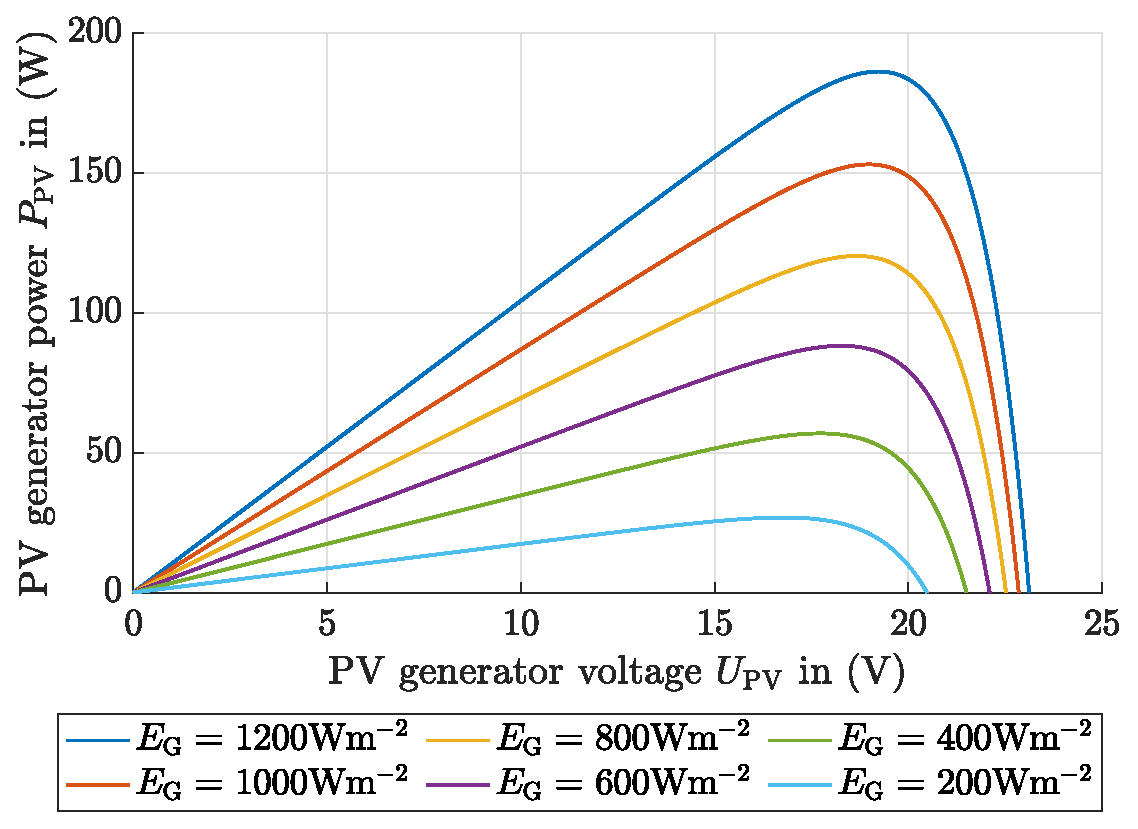
\includegraphics[width = 0.67\textwidth]{image_power_volt_irr_das_energy.eps}
  	\caption{Modeled power-voltage characteristic of the DAS Energy DAS145PF PV generator, depending on the total irradiance onto its inclined surface $E_\mathrm{G}$. The PV cell temperature $\vartheta_\mathrm{C} = 25^\circ\mathrm{C}$ is assumed to be constant.}
	\label{fig:image_power_volt_irr_das_energy}
\end{figure}

Another interesting behavior of the PV generators can be observed for different temperatures $\vartheta_\mathrm{C}$ of their PV cells. Due to the temperature increse of the semiconductors, the current $I_\mathrm{Ph} = I_\mathrm{SC}$ increses, however not as much as the voltage $U_\mathrm{OC}$ decreses. 
\begin{figure}[h!]
	\centering
  	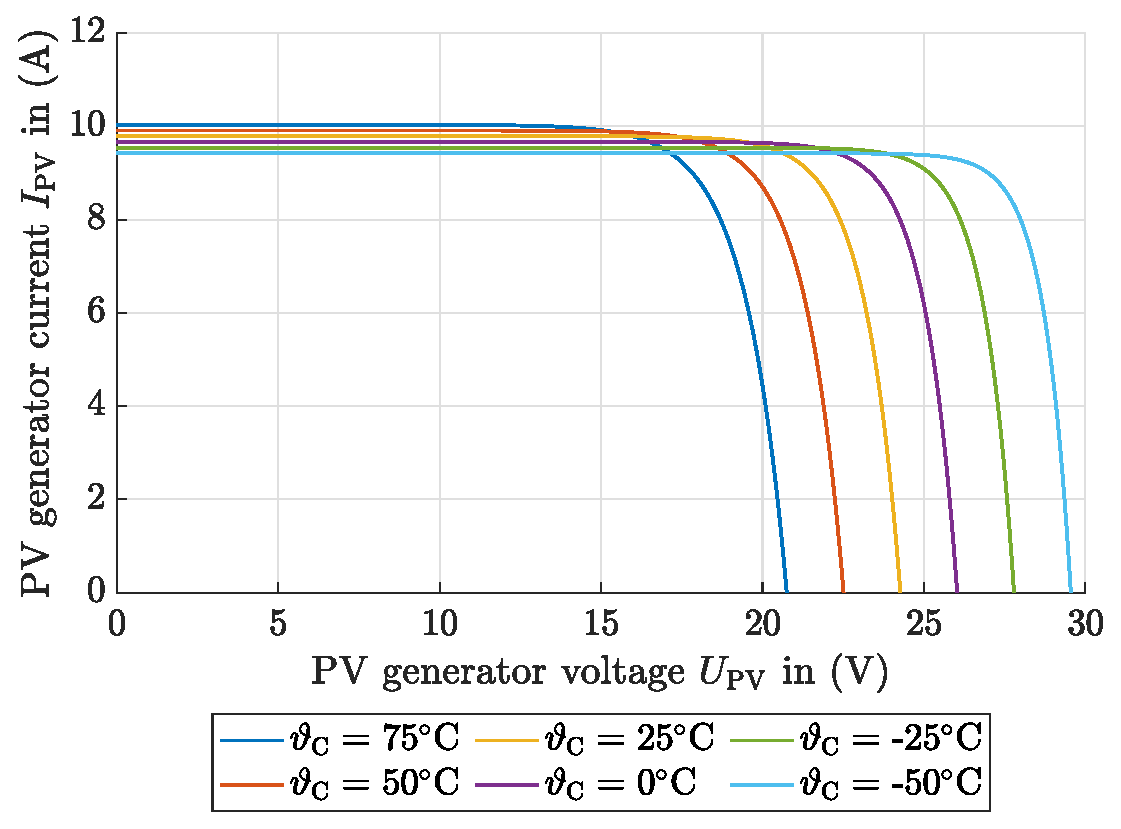
\includegraphics[width = 0.67\textwidth]{image_curr_volt_temp_ae_solar.eps}
  	\caption{Modeled current-voltage characteristic of the AE Solar AE195SMM6-36 PV generator, depending on its PV cell temperature $\vartheta_\mathrm{C}$. The total irradiance onto its inclined surface $E_\mathrm{G} = 1000\mathrm{Wm}^{-2}$ is assumed to be constant.}
	\label{fig:image_curr_volt_temp_ae_solar}
\end{figure}
\begin{figure}[h!]
	\centering
  	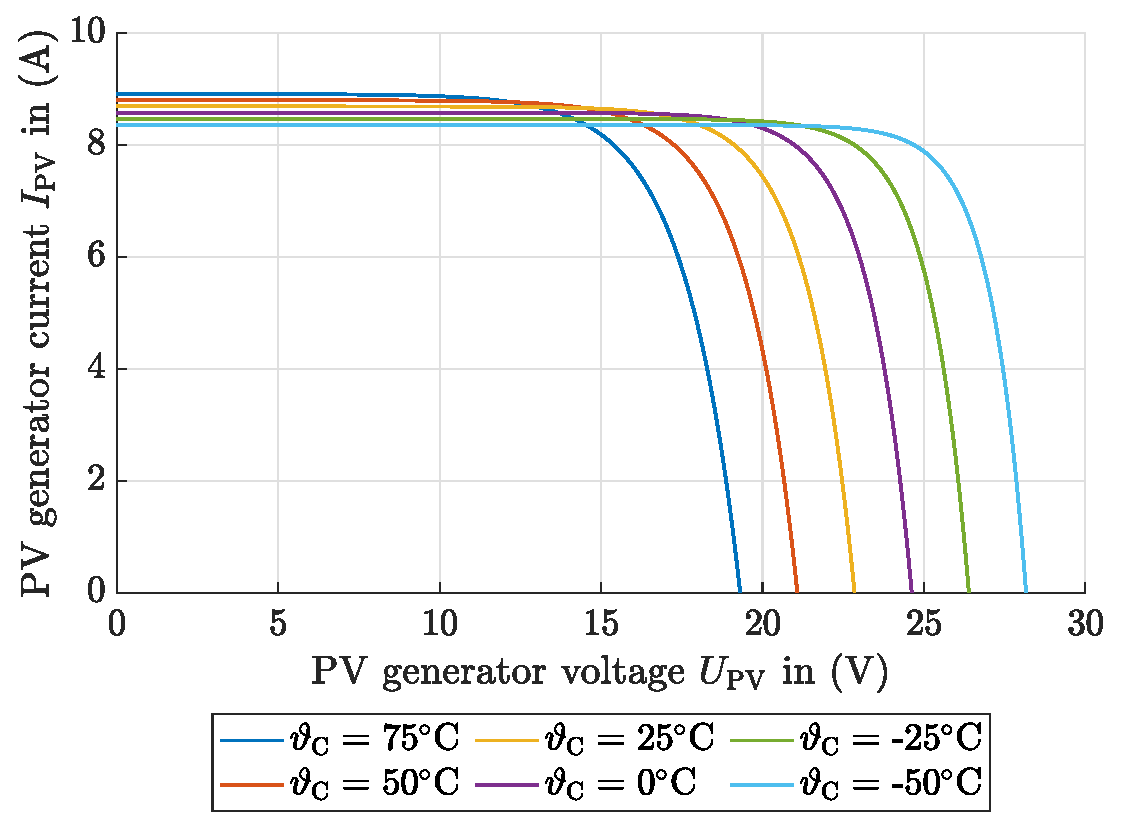
\includegraphics[width = 0.67\textwidth]{image_curr_volt_temp_das_energy.eps}
  	\caption{Modeled current-voltage characteristic of the DAS Energy DAS145PF PV generator, depending on its PV cell temperature $\vartheta_\mathrm{C}$. The total irradiance onto its inclined surface $E_\mathrm{G} = 1000\mathrm{Wm}^{-2}$ is assumed to be constant.}
	\label{fig:image_curr_volt_temp_das_energy}
\end{figure}
This finding results in an overall decrease in the power output $P_\mathrm{PV}$ of the PV generators for rising temperatures $\vartheta_\mathrm{C}$. Similarly, such behavior can be observed for decreasing temperatures $\vartheta_\mathrm{C}$. Here the overall power output $P_\mathrm{PV}$ increases. This is shown in the figures \ref{fig:image_curr_volt_temp_ae_solar} and \ref{fig:image_curr_volt_temp_das_energy}. When modeling a self-sufficient energy system, this factor must therefore not be neglected \cite{Mertens:2015}. 
\begin{figure}[h!]
	\centering
  	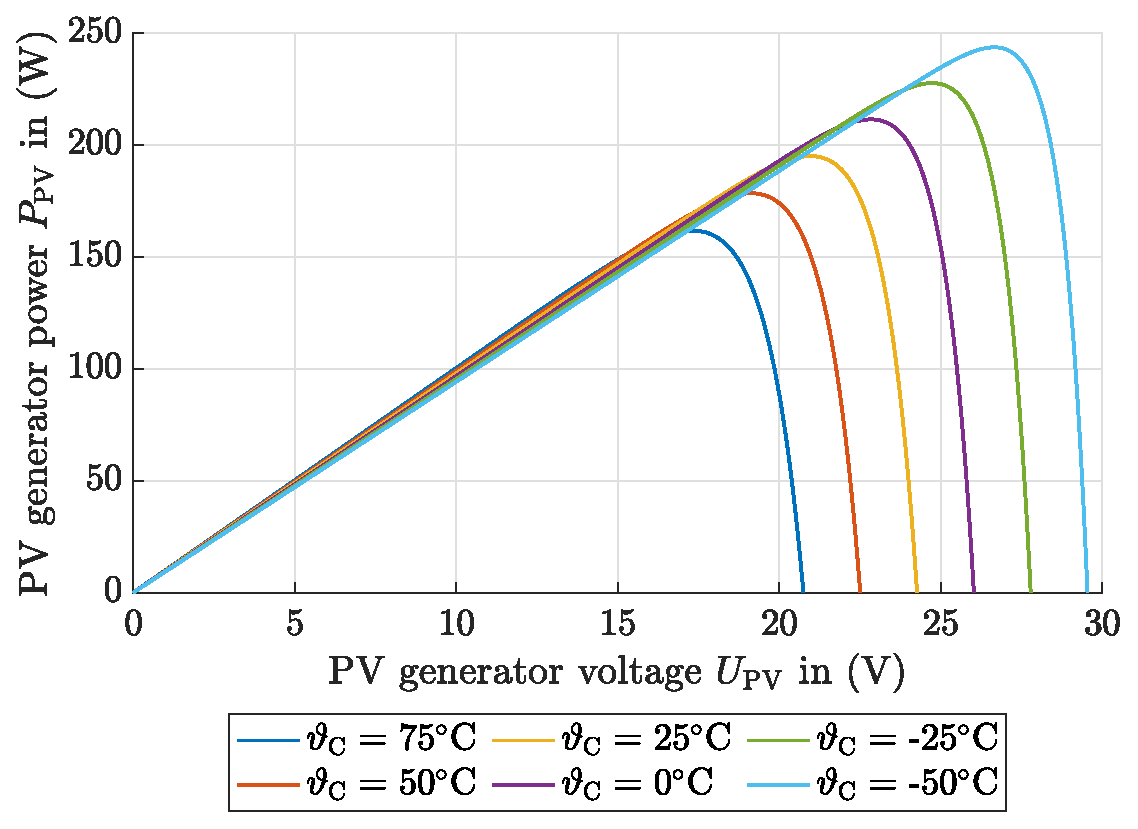
\includegraphics[width = 0.67\textwidth]{image_power_volt_temp_ae_solar.eps}
  	\caption{Modeled power-voltage characteristic of the AE Solar AE195SMM6-36 PV generator, depending on its PV cell temperature $\vartheta_\mathrm{C}$. The total irradiance onto its inclined surface $E_\mathrm{G} = 1000\mathrm{Wm}^{-2}$ is assumed to be constant.}
	\label{fig:image_power_volt_temp_ae_solar}
\end{figure}
\begin{figure}[h!]
	\centering
  	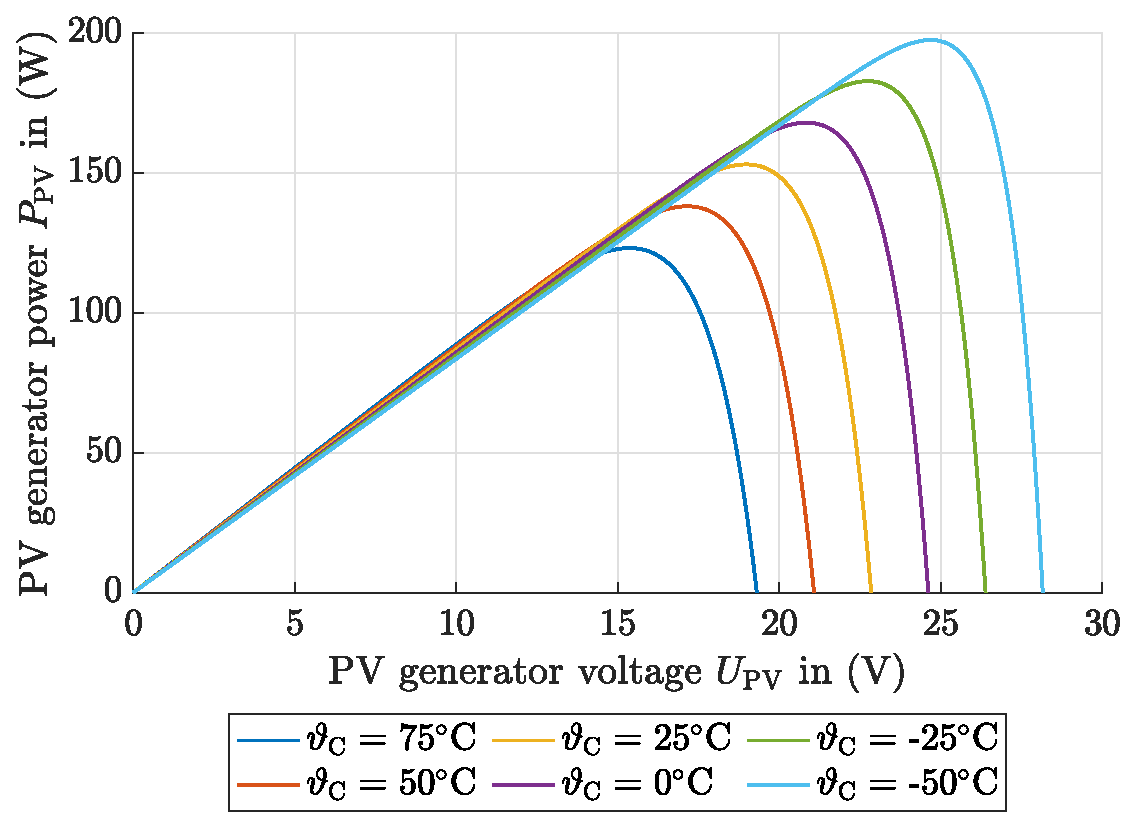
\includegraphics[width = 0.67\textwidth]{image_power_volt_temp_das_energy.eps}
  	\caption{Modeled power-voltage characteristic of the DAS Energy DAS145PF PV generator, depending on its PV cell temperature $\vartheta_\mathrm{C}$. The total irradiance onto its inclined surface $E_\mathrm{G} = 1000\mathrm{Wm}^{-2}$ is assumed to be constant.}
	\label{fig:image_power_volt_temp_das_energy}
\end{figure}

With the help of the aforementioned \MATLAB program, the ideality factors of the two PV generators were empirically determined in such a way that their power output at MPP for STCs corresponds to that in their data sheets. This resulted in an ideality factor of $m = 1,19045$ for the AE Solar AE195SMM6-36 PV generator and $m = 1,58972$ for the DAS Energy DAS145PF PV generator -- for an accuracy of two decimal places. 


 






\clearpage
\subsection{$\boldsymbol{\mathrm{LiFePO}_4}$ battery model} \label{sec_bat_res}
As already mentioned, the Offgridtec Smart-Pro $12,8\mathrm{V}$ $50\mathrm{Ah}$ $\mathrm{LiFePO_4}$ battery -- which from now on will simply be refered to as battery -- is used to store the electrical energy converted by the PV generator and to supply the repeater radio infrastructure with it. Table \ref{tab:table_smart_pro_lifepo4_battery} contains an excerpt from the data sheet for this battery, with which the nominal current of the battery can be calculated using the equation (\ref{eq:i_nom}) to $I_\mathrm{nom} = 16,67\mathrm{A}$. 
\begin{table}[h!]
	\centering
	\input{tables/table_smart_pro_lifepo4_battery}
	\caption{Excerpt from the data sheet of the Offgridtec Smart-Pro $12,8\mathrm{V}$ $50\mathrm{Ah}$ $\mathrm{LiFePO_4}$ battery \cite{Offgridtec:2020}.}
	\label{tab:table_smart_pro_lifepo4_battery}
\end{table}

So that this battery can be used with the \MATLAB simulation in the appendix \ref{sec:matlab_code}, the discharging and charging experiments discussed in the subsection \ref{sec:electrochemical} had to be carried out. The laboratory equipment required for these experiments is listed in the table \ref{tab:table_dis_chrg_exp_equipm}.
\begin{table}[h!]
	\centering
	\input{tables/table_dis_chrg_exp_equipm}
	\caption{Laboratory equipment required to carry out the discharging and charging experiment with the Offgridtec Smart-Pro $12,8\mathrm{V}$ $50\mathrm{Ah}$ $\mathrm{LiFePO_4}$ battery.}
	\label{tab:table_dis_chrg_exp_equipm}
\end{table}
A total of four electronic loads connected in parallel were used. This was done because each electronic load could only convert a maximum power of $60\mathrm{W}$ into heat. To assure that these were switched on and off at the same time, a central button for all electronic loads was used.

Before the experiments were carried out, the internal resistances of the input channels 1 and 2 of the oscilloscope were measured. These measurements resulted in $R_\mathrm{Ch1} = 1011,68\mathrm{k}\Omega$ for Ch1 and $R_\mathrm{Ch2} = 1004,99\mathrm{k}\Omega$ for Ch2. Taking into account the battery voltage $U_\mathrm{B}$ for the upper left and the current divider rule for the upper right loop in the figures \ref{fig:tikz_experiment_1} and \ref{fig:tikz_experiment_2}, it was determined that the resulting currents $I_\mathrm{Ch1}$ and $I_\mathrm{Ch2}$ are negligibly small. This applies because during the discharging experiment $I_\mathrm{L}$ was set so that $I_\mathrm{D}$ is equal to $I_\mathrm{nom}$ and during the charging experiment the battery charger provides a current of $I_\mathrm{BC} = 12\mathrm{A}$ \cite{MeanWell}. It is noted that neglecting $I_\mathrm{Ch1}$ and $I_\mathrm{Ch2}$ has the consequence that $I_\mathrm{D} = I_\mathrm{L}$ and $I_\mathrm{C} = I_\mathrm{BC}$.

Both experiments were carried out in such a way that measuring points were recorded in $0,05$ steps of the SOC. Thus, $N_\mathrm{MP} = 21$ measuring points had to be recorded per experiment. Based on this -- while taking into account the equation (\ref{eq:battery_charge}) and that $\eta_\mathrm{C} = 1$ -- the equations (\ref{eq:delta_t_D}) and (\ref{eq:delta_t_C}) result in $\Delta t_\mathrm{D} = 8,98\mathrm{min}$ and $\Delta t_\mathrm{C} = 12,5\mathrm{min}$. Since the battery has integrated Bluetooth, its SOC was additionally observed -- in parallel to a set timer -- using the Offgridtec Battery Viewer Smart Android app provided by Offgridtec GmbH.  
 
In order to get to the next measuring point, the battery had to be discharged with $I_\mathrm{D}$ over the time interval $\Delta t_\mathrm{D}$ or charged with $I_\mathrm{C}$ over the time interval $\Delta t_\mathrm{C}$. When this measuring point was reached, the currents were switched off. After 20min it could be clearly observed with Ch1 of the oscilloscope that the battery voltage hardly changed. Therefore $t_\mathrm{rest}$ was set to this time. At each measuring point the ambient temperature $\vartheta_\mathrm{A}$ was measured with a Newentor weather station (ASIN: B08M6C4MCM). This resulted in a \emph{mean ambient temperature} during the discharging experiment of $\overline{\vartheta}_\mathrm{A,D} = 23,99^\circ\mathrm{C}$ and during the charging experiment of $\overline{\vartheta}_\mathrm{A,C} = 25,23^\circ\mathrm{C}$.

Two recorded measurements for the discharging and charging experiment for $\mathrm{SOC}_n = 0,5$ can be seen in the figures \ref{fig:image_dis_50} and \ref{fig:image_chg_50}. The blue y-axes represent Ch1 and the green y-axes represent Ch2 of the oscilloscope. The green continuous lines are the currents $I_\mathrm{D}(t)$ and $I_\mathrm{C}(t)$ and the blue continuous lines are the battery voltages $U_\mathrm{B}(t)$ for the respective experiments. Furthermore, several cursors can be seen. In the case of the currents $I_\mathrm{D}(t)$ and $I_\mathrm{C}(t)$, the green dash-dotted cursor indicates their top value, and the green dashed cursor indicates their bottom value. In the case of the battery voltages $U_\mathrm{B}(t)$, the blue cursors mark the voltage drop for both experiments. The voltage drop instead of the voltage rise was used for the charging experiment because the observed rising slope was not steep enough -- after switching on $I_\mathrm{C}(t)$. This could falsify the result for calculating the electrolyte resistance $R_\mathrm{e,C}(\mathrm{SOC}_n)$. Similar to the currents, the blue dash-dotted cursor represents the top value of the voltage drop and the blue dashed cursor the bottom value of the voltage drop. 
\begin{figure}[h!]
	\centering
  	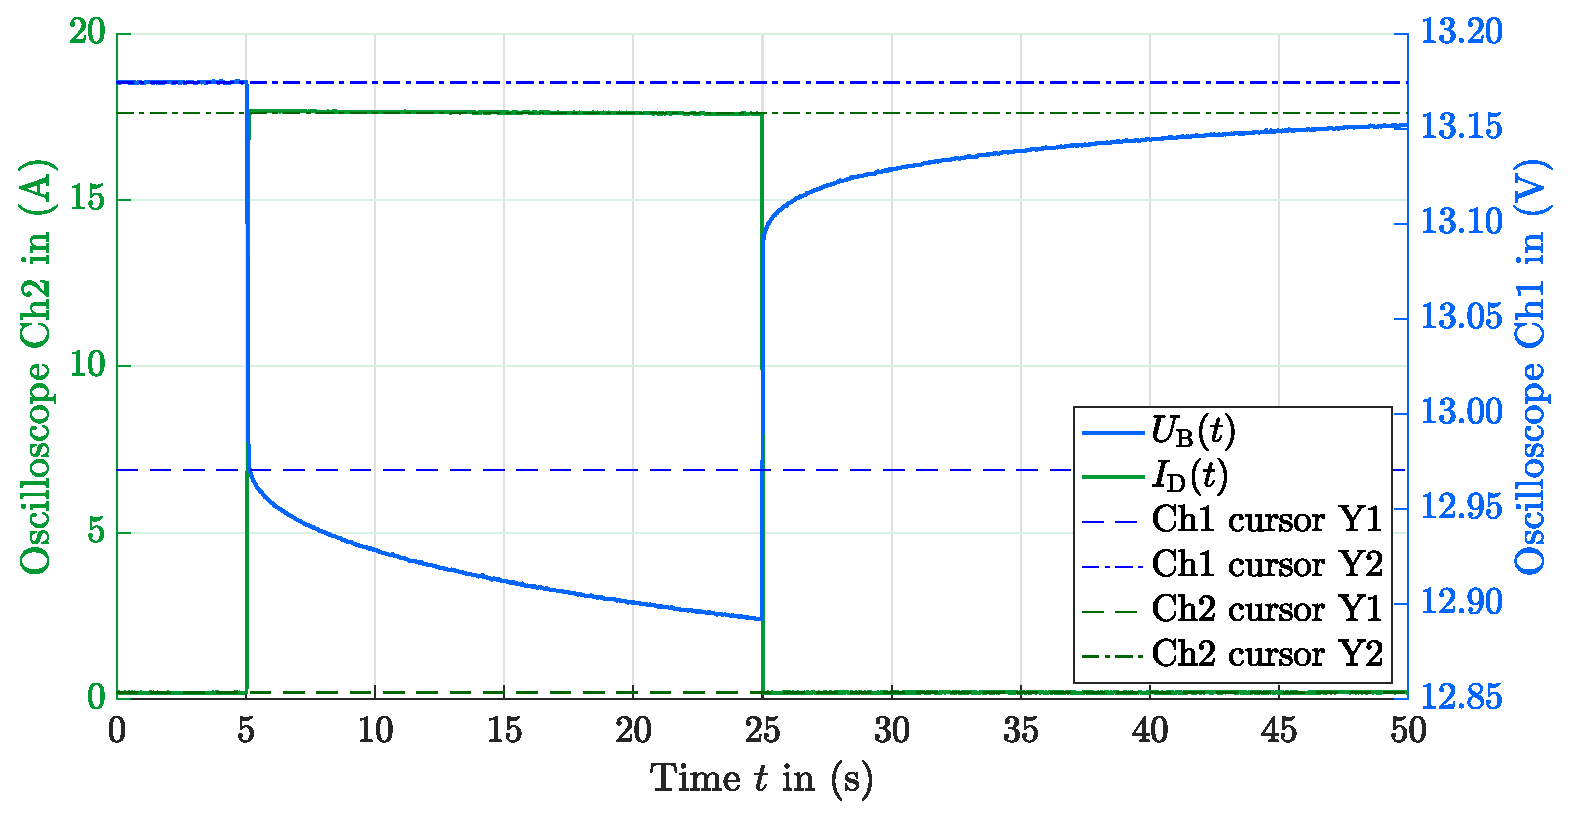
\includegraphics[width = 0.9\textwidth]{image_dis_50.eps}
  	\caption{Recorded time courses of $U_\mathrm{B}(t)$ and $I_\mathrm{D}(t)$ during the discharging experiment for $\mathrm{SOC}_n = 0,50$. The device under test was the Offgridtec Smart-Pro $12,8\mathrm{V}$ $50\mathrm{Ah}$ $\mathrm{LiFePO_4}$ battery.}
	\label{fig:image_dis_50}
\end{figure}
\begin{figure}[h!]
	\centering
  	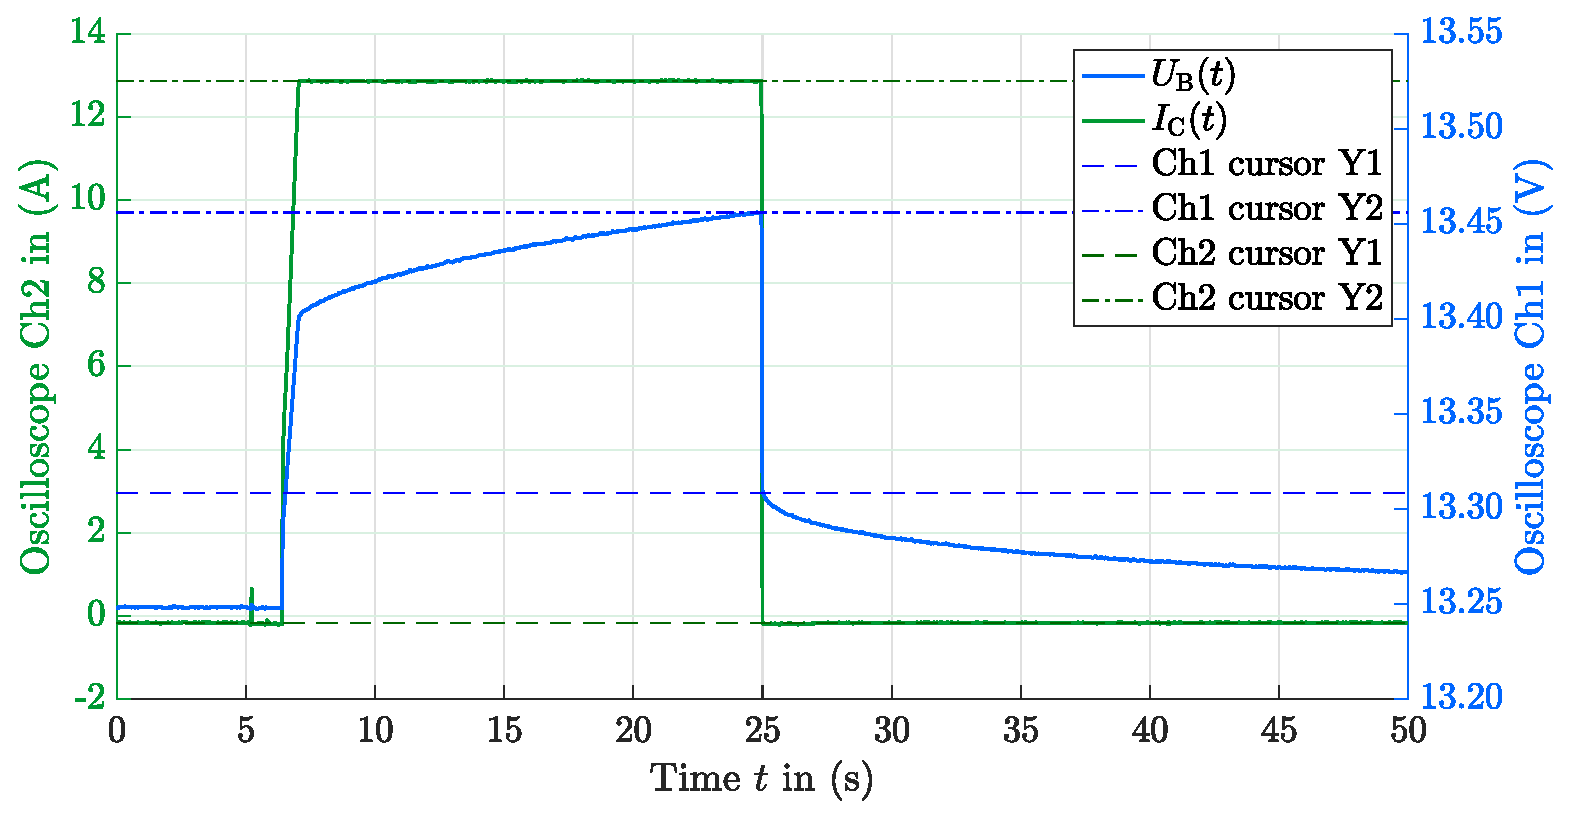
\includegraphics[width = 0.9\textwidth]{image_chg_50.eps}
	\caption{Recorded time courses of $U_\mathrm{B}(t)$ and $I_\mathrm{C}(t)$ during the charging experiment for $\mathrm{SOC}_n = 0,50$. The device under test was the Offgridtec Smart-Pro $12,8\mathrm{V}$ $50\mathrm{Ah}$ $\mathrm{LiFePO_4}$ battery.}
	\label{fig:image_chg_50}
\end{figure}

The time courses of the channels 1 and 2 shown in the figures \ref{fig:image_dis_50} and \ref{fig:image_chg_50} were recorded with the oscilloscope for all measuring points, with each being saved in a seperate\codeword{.cvs}file. Subsequently, the data in the\codeword{.cvs}files were processed with a \MATLAB program, in which the function\codeword{ischange()}was used to determine the positions of the cursors. The currents $I_\mathrm{D}(\mathrm{SOC}_n)$ and $I_\mathrm{C}(\mathrm{SOC}_n)$ as well as the voltage drops $\Delta U_\mathrm{D}(\mathrm{SOC}_n)$ and $\Delta U_\mathrm{C}(\mathrm{SOC}_n)$ were then calculated by subtracting their respective dashed cursor from their dash-dotted cursor. Now that all the required parameters were known, the electrolyte resistances $R_\mathrm{e,D}(\mathrm{SOC}_n)$ and $R_\mathrm{e,C}(\mathrm{SOC}_n)$ were determined using the equations (\ref{eq:r_0_d_soc}) and (\ref{eq:r_0_c_soc}).

For completeness it must be mentioned that the scales of the green y-axes from the figures \ref{fig:image_dis_50} and \ref{fig:image_chg_50} were calculated with this \MATLAB program by extracting the Ch2 data -- which represents the measured voltage drop across the shunt resistor -- from the\codeword{.cvs}files and applying it to the equations (\ref{eq_i_d_real}) and (\ref{eq:i_c_real}).

It should further be noted that $\Delta t_\mathrm{D}$ and $\Delta t_\mathrm{C}$ cannot be seen in the figures \ref{fig:image_dis_50} and \ref{fig:image_chg_50}, since these are the time intervals between two successive measuring points. The time interval between switching the discharging or charging current on and off -- for a certain measuring point -- was determined during the course of the experiments. When $t_\mathrm{rest}$ was over, the open-circuit voltages $U_\mathrm{0,D}(\mathrm{SOC}_n)$ and $U_\mathrm{0,C}(\mathrm{SOC}_n)$ were measured, the time scale of the oscilloscope was set to 50s and Ch1 was triggered manually. After approximately 5s, either the electronic load or the charger was switched on manually. After another 20s these were switched off again. This approach gave the best results. From the measured open-circuit voltages, $U_\mathrm{0}(\mathrm{SOC}_n)$ was calculated with the equation (\ref{eq:U_0}).

The results of the experiments are summarized in the table \ref{tab:table_exp_results} and visualized in the figures \ref{fig:image_open_circuit_voltages_matlab} and \ref{fig:image_electrolyte_resistances_matlab}. To obtain the battery model, these now only have to be interpolated and inserted into the equation (\ref{eq:battery_voltage_adapted}). 
\begin{table}[h!]
	\centering
	\input{tables/table_exp_results}
	\caption{Calculated results from the discharging and charging experiment carried out on the Offgridtec Smart-Pro $12,8\mathrm{V}$ $50\mathrm{Ah}$ $\mathrm{LiFePO_4}$ battery.}
	\label{tab:table_exp_results}
\end{table}
\begin{figure}[h!]
	\centering
  	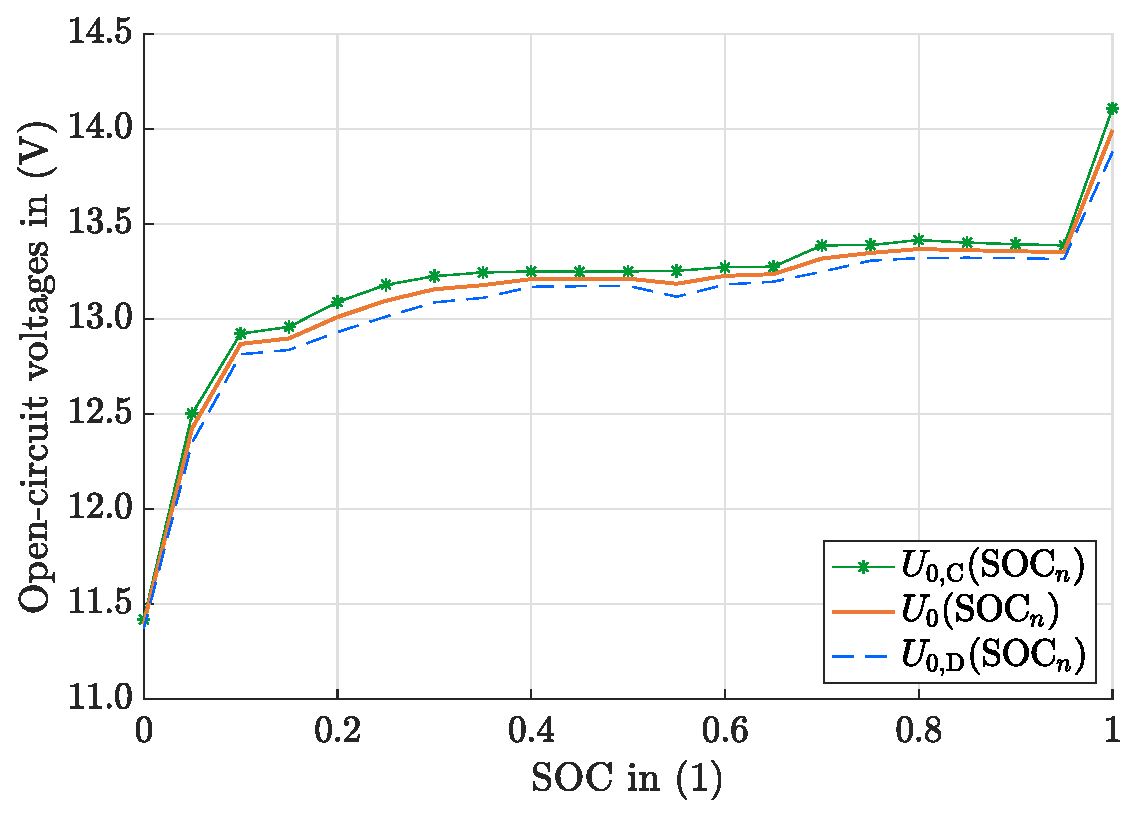
\includegraphics[width = 0.67\textwidth]{image_open_circuit_voltages_matlab.eps}
  	\caption{Open-circuit voltages $U_\mathrm{0,C}(\mathrm{SOC}_n)$, $U_\mathrm{0}(\mathrm{SOC}_n)$ and $U_\mathrm{0,D}(\mathrm{SOC}_n)$ obtained from the discharging and charging experiment carried out on the Offgridtec Smart-Pro $12,8\mathrm{V}$ $50\mathrm{Ah}$ $\mathrm{LiFePO_4}$ battery.}
	\label{fig:image_open_circuit_voltages_matlab}
\end{figure}
\begin{figure}[h!]
	\centering
  	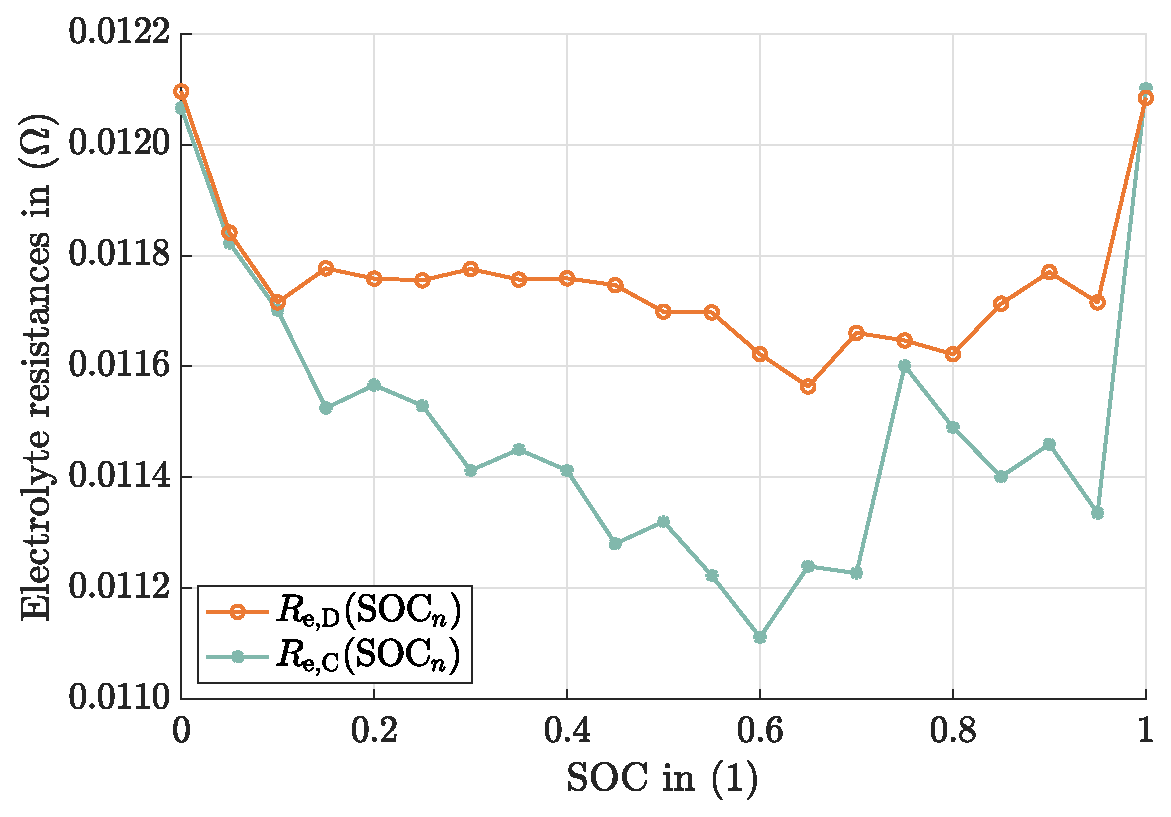
\includegraphics[width = 0.67\textwidth]{image_electrolyte_resistances_matlab.eps}
  	\caption{Electrolyte resistances $R_\mathrm{e,D}(\mathrm{SOC}_n)$ and $R_\mathrm{e,C}(\mathrm{SOC}_n)$ obtained from the discharging and charging experiment carried out on the Offgridtec Smart-Pro $12,8\mathrm{V}$ $50\mathrm{Ah}$ $\mathrm{LiFePO_4}$ battery.}
	\label{fig:image_electrolyte_resistances_matlab}
\end{figure}

Now it only remains to be shown that the assumptions for the equations (\ref{eq:battery_charge_cases}) and (\ref{current_cases}) are correct. For this purpose, the course of the charging current $I_\mathrm{C}(t)$ during the CV charging phase was measured for $\mathrm{SOC} \approx 0,99$ -- which was monitored via the Offgridtec Battery Viewer Smart app -- with Ch2 of the oscilloscope. The result can be seen in the figure \ref{fig:image_tau_b_matlab}, with the red continuous line representing the measured charging current. 
\begin{figure}[h!]
	\centering
  	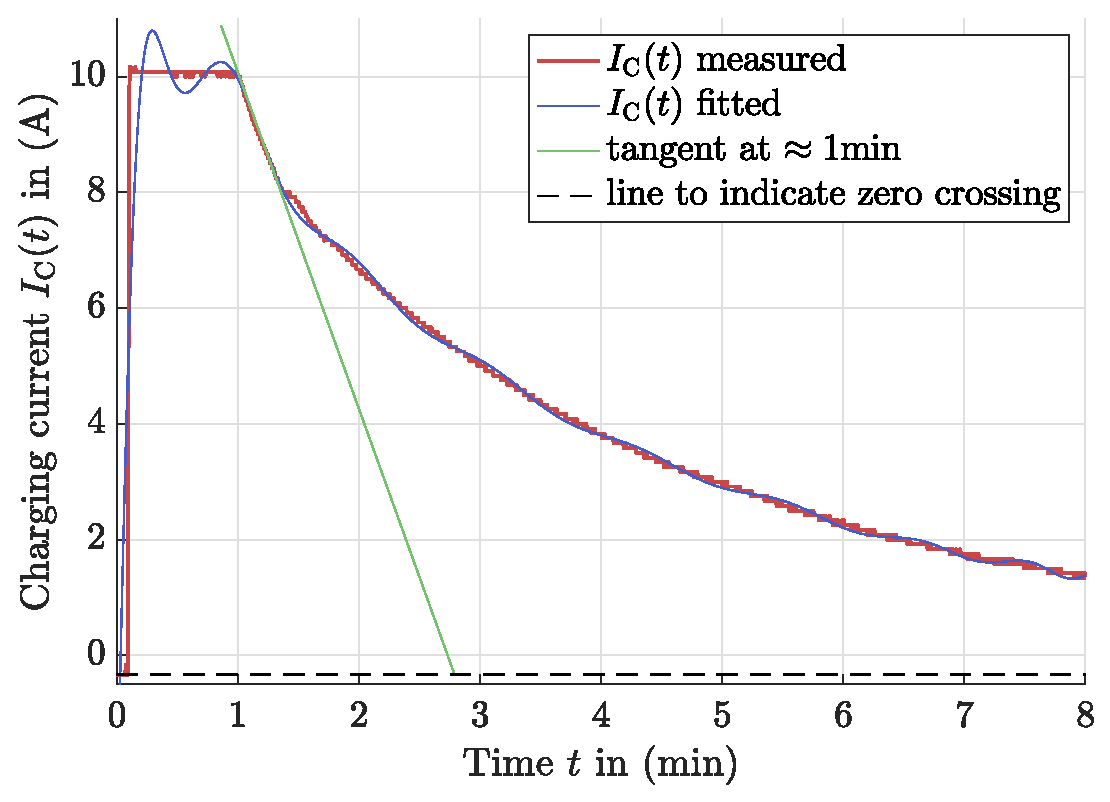
\includegraphics[width = 0.67\textwidth]{image_tau_b_matlab.eps}
  	\caption{Time course of $I_\mathrm{C}(t)$ over time during the CV charging phase of the Mean Well ENC-180-12 battery charger. The charged device was the Offgridtec Smart-Pro $12,8\mathrm{V}$ $50\mathrm{Ah}$ $\mathrm{LiFePO_4}$ battery.}
	\label{fig:image_tau_b_matlab}
\end{figure}
To prepare this measurement, the charging process of the almost fully charged battery ($\mathrm{SOC} \approx 0,99$) was switched off as soon as a decrease in the charging current was observed with Ch2 of the oscilloscope. This indicated that the battery charger was transitioning from the CC to the CV charging phase. Thereafter the battery was left to rest for 20min. The measurement was then recorded by setting the time scale of the oszilloscope to 8min, triggering Ch2 manually and continuing the charging process. First, the battery charger went into the CC charging phase and then, $t_1 = 1 \mathrm{min}$ after the start of the measurement, into the CV charging phase. No steep drop in the charging current can be seen from the recorded measurement (compare to figure \ref{fig:image_tau_b_matlab}). Thus, the described model for charging and discharging the battery from the equations (\ref{eq:battery_charge_cases}) and (\ref{current_cases}) is used for the \MATLAB simulation in the appendix \ref{sec:matlab_code}. 

As can be seen, the measured data was fitted with a polynomial function illustrated with the blue continuous line. The tangent of the polynomial fitting function, illustrated with the green continuous line, was chosen so that it runs through the point in time $t_1 = 1\mathrm{min}$ -- at which the battery charger changes from the CC to the CV charging phase. The top and bottom values of the charging current are $10,167\mathrm{A}$ and $-0,333\mathrm{A}$, with the difference between these values being the charging current in the CC charging phase $I_\mathrm{C} = 10,5\mathrm{A}$. Based on the bottom value, the black dashed line indicates the zero crossing of the measured $I_\mathrm{C}(t)$. The intersection with this line and the tangent is at $t_2 = 2,7904\mathrm{min}$. Hence, the measured time constant of the battery follows to:
\begin{equation}\label{eq:tau_battery_measured}
	\centering
	\tau_\mathrm{B} = t_2 - t_1 = 1,7904\mathrm{min}\text{.}
\end{equation}

It can be seen from the figures \ref{fig:image_dis_50}, \ref{fig:image_chg_50} and \ref{fig:image_tau_b_matlab} that the top and bottom values for the currents $I_\mathrm{D}$ and $I_\mathrm{C}$ do not quite match the values $I_\mathrm{nom}$ and $I_\mathrm{BC}$. This is likely due to the electronic loads and the battery charger. Since the behavior of these devices is only known from their data sheets, further investigations must be carried out in order to obtain more precise results. Alternatively, more professional devices that are certified for laboratory use can be used. Finally, a resistance measurement of the shunt resistor can be carried out in order to determine its exact resistance value.

\subsection{Performance estimation}
Now the results of the performance estimation of the self-sufficient energy distribution system for two different mission locations on Earth are presented. First for the Negev Desert in Israel, as the OeWF's next analog Mars field mission AMADEE-20 will take place there from October 4\textsuperscript{th} to October 31\textsuperscript{st}, 2021, and then for Vienna, Austria, from April 1\textsuperscript{st} to April 30\textsuperscript{th}, as this is the location where the assembled voice communication system will probably be tested.

Before the simulated results are presented, the SCC must first be briefly introduced. For the self-sufficient energy distribution system, the Victron Energy BlueSolar MPPT 75/10 solar charging controller is used. Its specifications are listed in the table \ref{tab:table_scc_specs}.
\begin{table}[h!]
	\centering
	\input{tables/table_scc_specs}
	\caption{Excerpt from the user manual of the Victron Energy BlueSolar MPPT 75/10 solar charging controller \cite{Victron:2021}.}
	\label{tab:table_scc_specs}
\end{table}
According to the user manual of this SCC, it only connects the PV generator when a voltage of $U_\mathrm{in,PV} > U_\mathrm{B} + 5\mathrm{V}$ is reached at its PV generator input terminal. It is noted that $U_\mathrm{in,PV}$ already takes the cable losses into account. After this condition is met, the PV generator remains connected to the battery and the load as long as the new condition $U_\mathrm{in,PV} > U_\mathrm{B} + 1\mathrm{V}$ is fulfilled. In its user manual it is also mentioned that the maximum power of the PV generator must not exceed $145\mathrm{W}$. If the power is exceeded, the SCC limits the current from said generator \cite{Victron:2021}.

The \MATLAB simulation in the appendix \ref{sec:matlab_code} is based on the user manual of the Victron BlueSolar MPPT 75/10 SCC, the results presented in the subsections \ref{sec:pv_gen_mod} and \ref{sec_bat_res} and the basics explained in the section \ref{sec:solar_energy}.

Although it was mentioned in the subsection \ref{sec:load_radio} that a step function can be implemented for the load current, this was not successful in \MATLAB. It should also be noted that the battery charging process explained in the subsection \ref{sec:electrochemical} was not implemented due to the effort involved. Instead, the equation \ref{eq:soc} was used, which models a linear increase or decrease in the SOC of the battery. 

The aim of the \MATLAB simulation is to calculate how the PV generator must be installed at the mission location so that it can maximize its daily electrical energy yield throughout the mission. Based on the daily electrical energy yield, the \MATLAB simulation calculates the SOC of the battery for each mission day. It then gives a feedback if the the battery can be fully charged during the course of the mission. If this is the case, it is likely that the repeater radio system can be supplied with enough electrical energy. However, if the battery cannot be fully charged during the course of the mission, one or more PV generators must be connected in parallel to the existing one to increase the current $I_\mathrm{MPP}$, and thus $P_\mathrm{MPP}$, of the PV generator array \cite{Mertens:2015}. For completenss it is noted that the \MATLAB simulation assumes that the PV generators connected in parallel are the same type. In addition to that, the simulation can throw several error messages if either the conditions in the equations \ref{eq:h_sunrise} and \ref{eq:h_sunset} are not met, the voltage at the repeater is too low or to high, or if the battery gets fully discharged during the course of the mission.

Based on the simulation inputs for the Negev Desert in Israel and for Vienna, Austria, in the tables \ref{tab:table_negev} and \ref{tab:table_vienna}, the command window outputs of the \MATLAB simulation result in the listings \ref{lst:list_negev_1} and \ref{lst:list_negev_2} for the Negev Desert and in the listings \ref{lst:list_negev_3} and \ref{lst:list_negev_4} for Vienna. The global horizontal irradiation, direct normal irradiation and average ambient temperature for the Negev Desert can be obtained from the figures \ref{fig:temp_negev} to \ref{fig:dni_israel} and for Vienna from the figures \ref{fig:ghi_austria}, \ref{fig:dni_austria} and \ref{fig:temp_vienna}. %% CHANGE TABLES IF NECESSARY 
\begin{table}[h!]
	\centering
	\input{tables/table_negev}
	\caption{Input for the \MATLAB simulation of the self-sufficient energy distribution system for the Negev Desert in Israel.}
	\label{tab:table_negev}
\end{table}
\begin{table}[h!]
	\centering
	\input{tables/table_vienna}
	\caption{Input for the \MATLAB simulation of the self-sufficient energy distribution system for Vienna, Austria.}
	\label{tab:table_vienna}
\end{table}
\begin{figure}[h!]
	\centering
  	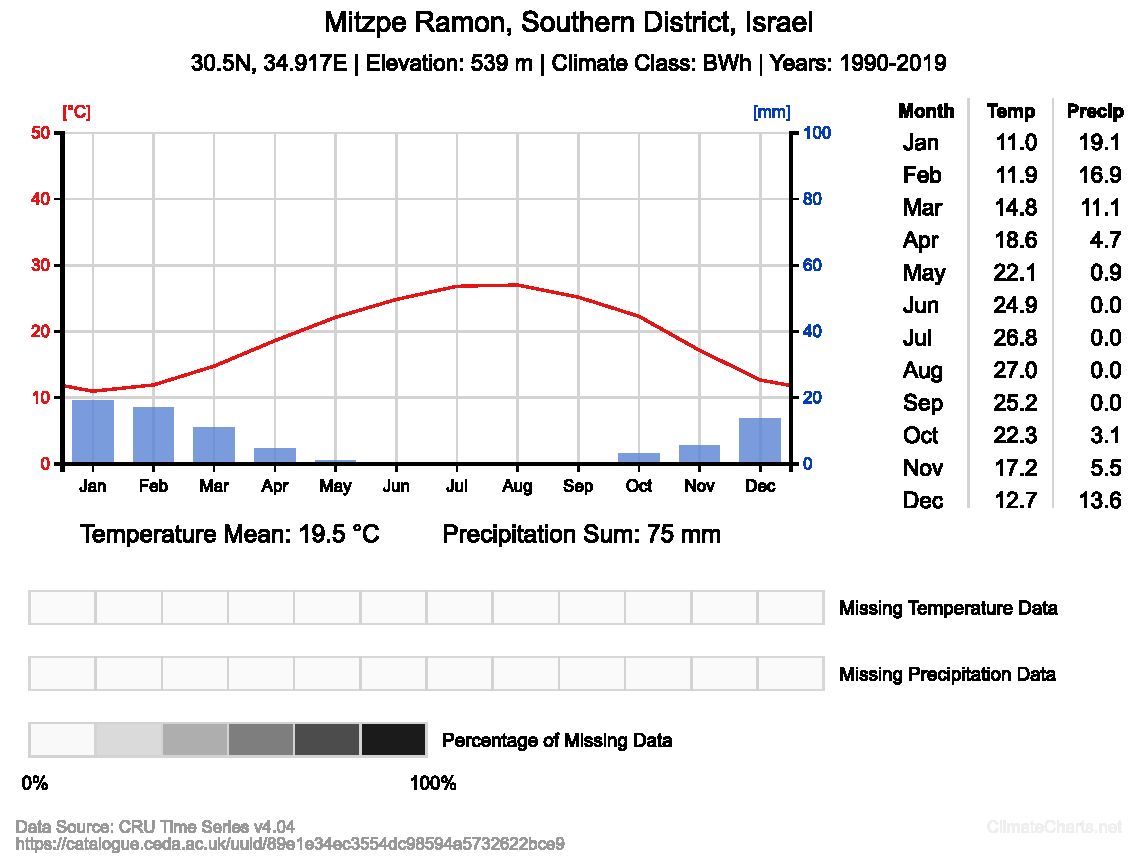
\includegraphics[width = 0.96\textwidth]{temp_maps/temp_negev}
  	\caption{Monthly averages of temperature and precipitation data for Mitzpe Ramon, Southern District, Israel (Negev Desert). (Image credit: \cite{Zepner:2020})}
	\label{fig:temp_negev}
\end{figure}

\begin{lstfloat}
\begin{lstlisting}[numbers = none, caption = {Output of the \MATLAB simulation in appendix \ref{sec:matlab_code} regarding the installation of the PV generator for the mission inputs in the table \ref{tab:table_negev}.}, label = lst:list_negev_1, captionpos = b]
              *******************************************
              [OUTPUT] PV GENERATOR INSTALLATION:

              Mission day | Opt. tilt angle | Orientation
              -------------------------------------------
              04-Oct-2021 |    35.78 deg    |    SOUTH
              05-Oct-2021 |    36.18 deg    |    SOUTH
              06-Oct-2021 |    36.57 deg    |    SOUTH
              07-Oct-2021 |    36.96 deg    |    SOUTH
              08-Oct-2021 |    37.34 deg    |    SOUTH
              09-Oct-2021 |    37.73 deg    |    SOUTH
              10-Oct-2021 |    38.11 deg    |    SOUTH
              11-Oct-2021 |    38.49 deg    |    SOUTH
              12-Oct-2021 |    38.87 deg    |    SOUTH
              13-Oct-2021 |    39.25 deg    |    SOUTH
              14-Oct-2021 |    39.62 deg    |    SOUTH
              15-Oct-2021 |    39.99 deg    |    SOUTH
              16-Oct-2021 |    40.36 deg    |    SOUTH
              17-Oct-2021 |    40.72 deg    |    SOUTH
              18-Oct-2021 |    41.08 deg    |    SOUTH
              19-Oct-2021 |    41.44 deg    |    SOUTH
              20-Oct-2021 |    41.80 deg    |    SOUTH
              21-Oct-2021 |    42.15 deg    |    SOUTH
              22-Oct-2021 |    42.50 deg    |    SOUTH
              23-Oct-2021 |    42.84 deg    |    SOUTH
              24-Oct-2021 |    43.18 deg    |    SOUTH
              25-Oct-2021 |    43.52 deg    |    SOUTH
              26-Oct-2021 |    43.86 deg    |    SOUTH
              27-Oct-2021 |    44.19 deg    |    SOUTH
              28-Oct-2021 |    44.51 deg    |    SOUTH
              29-Oct-2021 |    44.83 deg    |    SOUTH
              30-Oct-2021 |    45.15 deg    |    SOUTH
              31-Oct-2021 |    45.46 deg    |    SOUTH
              -------------------------------------------
                  Mean    |    40.80 deg    |    SOUTH

              *******************************************
\end{lstlisting}
\end{lstfloat}
Listing \ref{lst:list_negev_1} shows the optimal angle of inclination -- or tilting angle -- $\beta$ and the orientation of the normal to the PV generator's energy converting surface $A_\mathrm{PV}$, with respect to the cardinal directions, for each mission day. As explained in the subsection \ref{sec:photovoltaic_generator_alignment}, the optimal angle of inclination applies for solar noon $t_\mathrm{S} = 12\mathrm{h}$. This might not be true for cloudy days when the direct normal irradiation is weaker. During these days, $\beta$ must be reduced in order to maximize $E_\mathrm{DIFG}$ and $E_\mathrm{RGI}$ (copmare to equations \ref{eq:e_difg} and \ref{eq:e_rgi}), which causes $E_\mathrm{G}$ to increse (compare to equation \ref{eq:e_gen_ghi_dni}). Furthermore, the simulation determines the mean angle of inclination and orientation so that the PV generator only needs to be set up once at the beginning of the mission.

\begin{lstfloat}
\begin{lstlisting}[keywordstyle=\color{black}, numbers = none, caption = {Output of the \MATLAB simulation in appendix \ref{sec:matlab_code} regarding the daily energy yield of the PV generator for the mission inputs in the table \ref{tab:table_negev}.}, label = lst:list_negev_2, captionpos = b]
                 *************************************
                 [OUTPUT] PV GENERATOR ENERGY YIELD:

                 Applies for mean tilting angle and
                 orientation. The energy yield is 
                 the electrical energy yield. SOC 
                 full shows if the battery could be 
                 fully charged during the day.

                 Mission day | Energy yield | SOC full
                 -------------------------------------
                 04-Oct-2021 |   427.74 Wh  |    NO   
                 05-Oct-2021 |   428.65 Wh  |    NO   
                 06-Oct-2021 |   430.23 Wh  |    NO   
                 07-Oct-2021 |   431.09 Wh  |    NO   
                 08-Oct-2021 |   431.92 Wh  |    NO   
                 09-Oct-2021 |   433.41 Wh  |    NO   
                 10-Oct-2021 |   434.17 Wh  |   YES   
                 11-Oct-2021 |   435.61 Wh  |   YES   
                 12-Oct-2021 |   436.31 Wh  |   YES   
                 13-Oct-2021 |   437.69 Wh  |   YES   
                 14-Oct-2021 |   438.32 Wh  |   YES   
                 15-Oct-2021 |   439.64 Wh  |   YES   
                 16-Oct-2021 |   440.21 Wh  |   YES   
                 17-Oct-2021 |   441.46 Wh  |   YES   
                 18-Oct-2021 |   441.96 Wh  |   YES   
                 19-Oct-2021 |   443.15 Wh  |   YES   
                 20-Oct-2021 |   443.58 Wh  |   YES   
                 21-Oct-2021 |   444.71 Wh  |   YES   
                 22-Oct-2021 |   445.80 Wh  |   YES   
                 23-Oct-2021 |   446.12 Wh  |   YES   
                 24-Oct-2021 |   447.15 Wh  |   YES   
                 25-Oct-2021 |   447.40 Wh  |   YES   
                 26-Oct-2021 |   448.37 Wh  |   YES   
                 27-Oct-2021 |   449.30 Wh  |   YES   
                 28-Oct-2021 |   449.44 Wh  |   YES   
                 29-Oct-2021 |   450.30 Wh  |   YES   
                 30-Oct-2021 |   450.37 Wh  |   YES   
                 31-Oct-2021 |   451.16 Wh  |   YES   

                 *************************************
\end{lstlisting}
\end{lstfloat}
To display the command window output shown in the listing \ref{lst:list_negev_2}, the simulation uses the mean inclination angle from the listing \ref{lst:list_negev_1} and calculates the daily electrical energy yield of the PV generator. On the basis of this, the SOC of the battery is calculated for each mission day. An algorithm then evaluates whether the battery has been fully charged during each mission day and outputs either \codeword{YES} or \codeword{NO}. As it can be seen, the battery cannot be fully charged for the first few mission days. This is due to the assumption that the battery is $60\%$ charged at the beginning of the mission -- hence $\mathrm{SOC_{init}} = 0,6$. With this SOC, the Offgridtec Smart-Pro $12,8\mathrm{V}$ $50\mathrm{Ah}$ $\mathrm{LiFePO}_4$ battery is stored for longer periods of time \cite{Offgridtec:2020}. Therefore it can be said that the self-sufficient energy distribution system can supply the repeater radio system during the course of the analog Mars field mission AMADEE-20.

An interesting case occurs when the battery cannot be fully charged towards the end of the mission. This can happen, for instance, when the available solar energy is decreasing every day. Such results can be explained by changing seasons. In this case PV generators must be connected in parallel to guarantee sufficient electrical energy supply of the repeater radio system throughout the mission.

\begin{lstfloat}
\begin{lstlisting}[numbers = none, caption = {Output of the \MATLAB simulation in appendix \ref{sec:matlab_code} regarding the installation of the PV generator for the mission inputs in the table \ref{tab:table_vienna}.}, label = lst:list_negev_3, captionpos = b]
              *******************************************
              [OUTPUT] PV GENERATOR INSTALLATION:

              Mission day | Opt. tilt angle | Orientation
              -------------------------------------------
              01-Apr-2021 |    43.84 deg    |    SOUTH
              02-Apr-2021 |    43.44 deg    |    SOUTH
              03-Apr-2021 |    43.05 deg    |    SOUTH
              04-Apr-2021 |    42.65 deg    |    SOUTH
              05-Apr-2021 |    42.26 deg    |    SOUTH
              06-Apr-2021 |    41.87 deg    |    SOUTH
              07-Apr-2021 |    41.48 deg    |    SOUTH
              08-Apr-2021 |    41.10 deg    |    SOUTH
              09-Apr-2021 |    40.71 deg    |    SOUTH
              10-Apr-2021 |    40.33 deg    |    SOUTH
              11-Apr-2021 |    39.95 deg    |    SOUTH
              12-Apr-2021 |    39.58 deg    |    SOUTH
              13-Apr-2021 |    39.20 deg    |    SOUTH
              14-Apr-2021 |    38.83 deg    |    SOUTH
              15-Apr-2021 |    38.46 deg    |    SOUTH
              16-Apr-2021 |    38.10 deg    |    SOUTH
              17-Apr-2021 |    37.74 deg    |    SOUTH
              18-Apr-2021 |    37.38 deg    |    SOUTH
              19-Apr-2021 |    37.02 deg    |    SOUTH
              20-Apr-2021 |    36.67 deg    |    SOUTH
              21-Apr-2021 |    36.32 deg    |    SOUTH
              22-Apr-2021 |    35.97 deg    |    SOUTH
              23-Apr-2021 |    35.63 deg    |    SOUTH
              24-Apr-2021 |    35.29 deg    |    SOUTH
              25-Apr-2021 |    34.95 deg    |    SOUTH
              26-Apr-2021 |    34.62 deg    |    SOUTH
              27-Apr-2021 |    34.30 deg    |    SOUTH
              28-Apr-2021 |    33.97 deg    |    SOUTH
              29-Apr-2021 |    33.65 deg    |    SOUTH
              30-Apr-2021 |    33.34 deg    |    SOUTH
              -------------------------------------------
                  Mean    |    38.39 deg    |    SOUTH

              *******************************************
\end{lstlisting}
\end{lstfloat}
\begin{lstfloat}
\begin{lstlisting}[keywordstyle=\color{black}, numbers = none, caption = {Output of the \MATLAB simulation in appendix \ref{sec:matlab_code} regarding the daily energy yield of the PV generator for the mission inputs in the table \ref{tab:table_vienna}.}, label = lst:list_negev_4, captionpos = b]
                 *************************************
                 [OUTPUT] PV GENERATOR ENERGY YIELD:

                 Applies for mean tilting angle and
                 orientation. The energy yield is 
                 the electrical energy yield. SOC
                 full shows if the battery could be
                 fully charged during the day.

                 Mission day | Energy yield | SOC full
                 -------------------------------------
                 01-Apr-2021 |   490.62 Wh  |    NO   
                 02-Apr-2021 |   490.80 Wh  |    NO   
                 03-Apr-2021 |   490.98 Wh  |   YES   
                 04-Apr-2021 |   491.15 Wh  |   YES   
                 05-Apr-2021 |   491.31 Wh  |   YES   
                 06-Apr-2021 |   491.47 Wh  |   YES   
                 07-Apr-2021 |   491.62 Wh  |   YES   
                 08-Apr-2021 |   491.78 Wh  |   YES   
                 09-Apr-2021 |   491.93 Wh  |   YES   
                 10-Apr-2021 |   492.08 Wh  |   YES   
                 11-Apr-2021 |   492.23 Wh  |   YES   
                 12-Apr-2021 |   492.38 Wh  |   YES   
                 13-Apr-2021 |   492.53 Wh  |   YES   
                 14-Apr-2021 |   491.98 Wh  |   YES   
                 15-Apr-2021 |   492.16 Wh  |   YES   
                 16-Apr-2021 |   492.32 Wh  |   YES   
                 17-Apr-2021 |   492.48 Wh  |   YES   
                 18-Apr-2021 |   492.65 Wh  |   YES   
                 19-Apr-2021 |   492.83 Wh  |   YES   
                 20-Apr-2021 |   493.01 Wh  |   YES   
                 21-Apr-2021 |   492.51 Wh  |   YES   
                 22-Apr-2021 |   492.73 Wh  |   YES   
                 23-Apr-2021 |   492.94 Wh  |   YES   
                 24-Apr-2021 |   493.16 Wh  |   YES   
                 25-Apr-2021 |   492.70 Wh  |   YES   
                 26-Apr-2021 |   492.94 Wh  |   YES   
                 27-Apr-2021 |   493.23 Wh  |   YES   
                 28-Apr-2021 |   492.80 Wh  |   YES   
                 29-Apr-2021 |   493.09 Wh  |   YES   
                 30-Apr-2021 |   493.40 Wh  |   YES   

                 *************************************
\end{lstlisting}
\end{lstfloat}
A similar command window output can be obtained from the listings \ref{lst:list_negev_3} and \ref{lst:list_negev_4} for Vienna. Here, however, two PV generators connected in parallel are required. Besides that, simulations have shown, that the daily electrical energy yield is incresed when the angle of inlcination $\beta = 0^\circ$. This can also be recognized by analyzing the solar resources maps in the figures \ref{fig:ghi_austria} and \ref{fig:dni_austria}, because the global horizontal irradiation is greater than the direct normal irradiation. The author of the book \cite{Mertens:2015} mentions this as well. Such a simulation result can further be explained by the fact that these solar resource maps provide average values that have been recorded over several years and are therefore mainly used for the long-term planning of a PV generator array.

In order to obtain more intuitive simulation results, the SOC of the battery can be plotted over the entire duration of the mission or for individual mission days. Since the \MATLAB simulation only serves as a reference point, the on-site support crew still has to make regular checks of the battery's SOC during the mission in order to collect empirical data. Finally, it should be noted that the simulation could not provide any results for the DAS Energy DAS145PF PV generator, as it could not meet the condition $U_\mathrm{in,PV} > U_\mathrm{B} + 5\mathrm{V}$ with the solar resource maps mentioned. However, this could be different with the solar resource maps from \cite{Union:2020}. 

\begin{figure}[h!]
	\centering
  	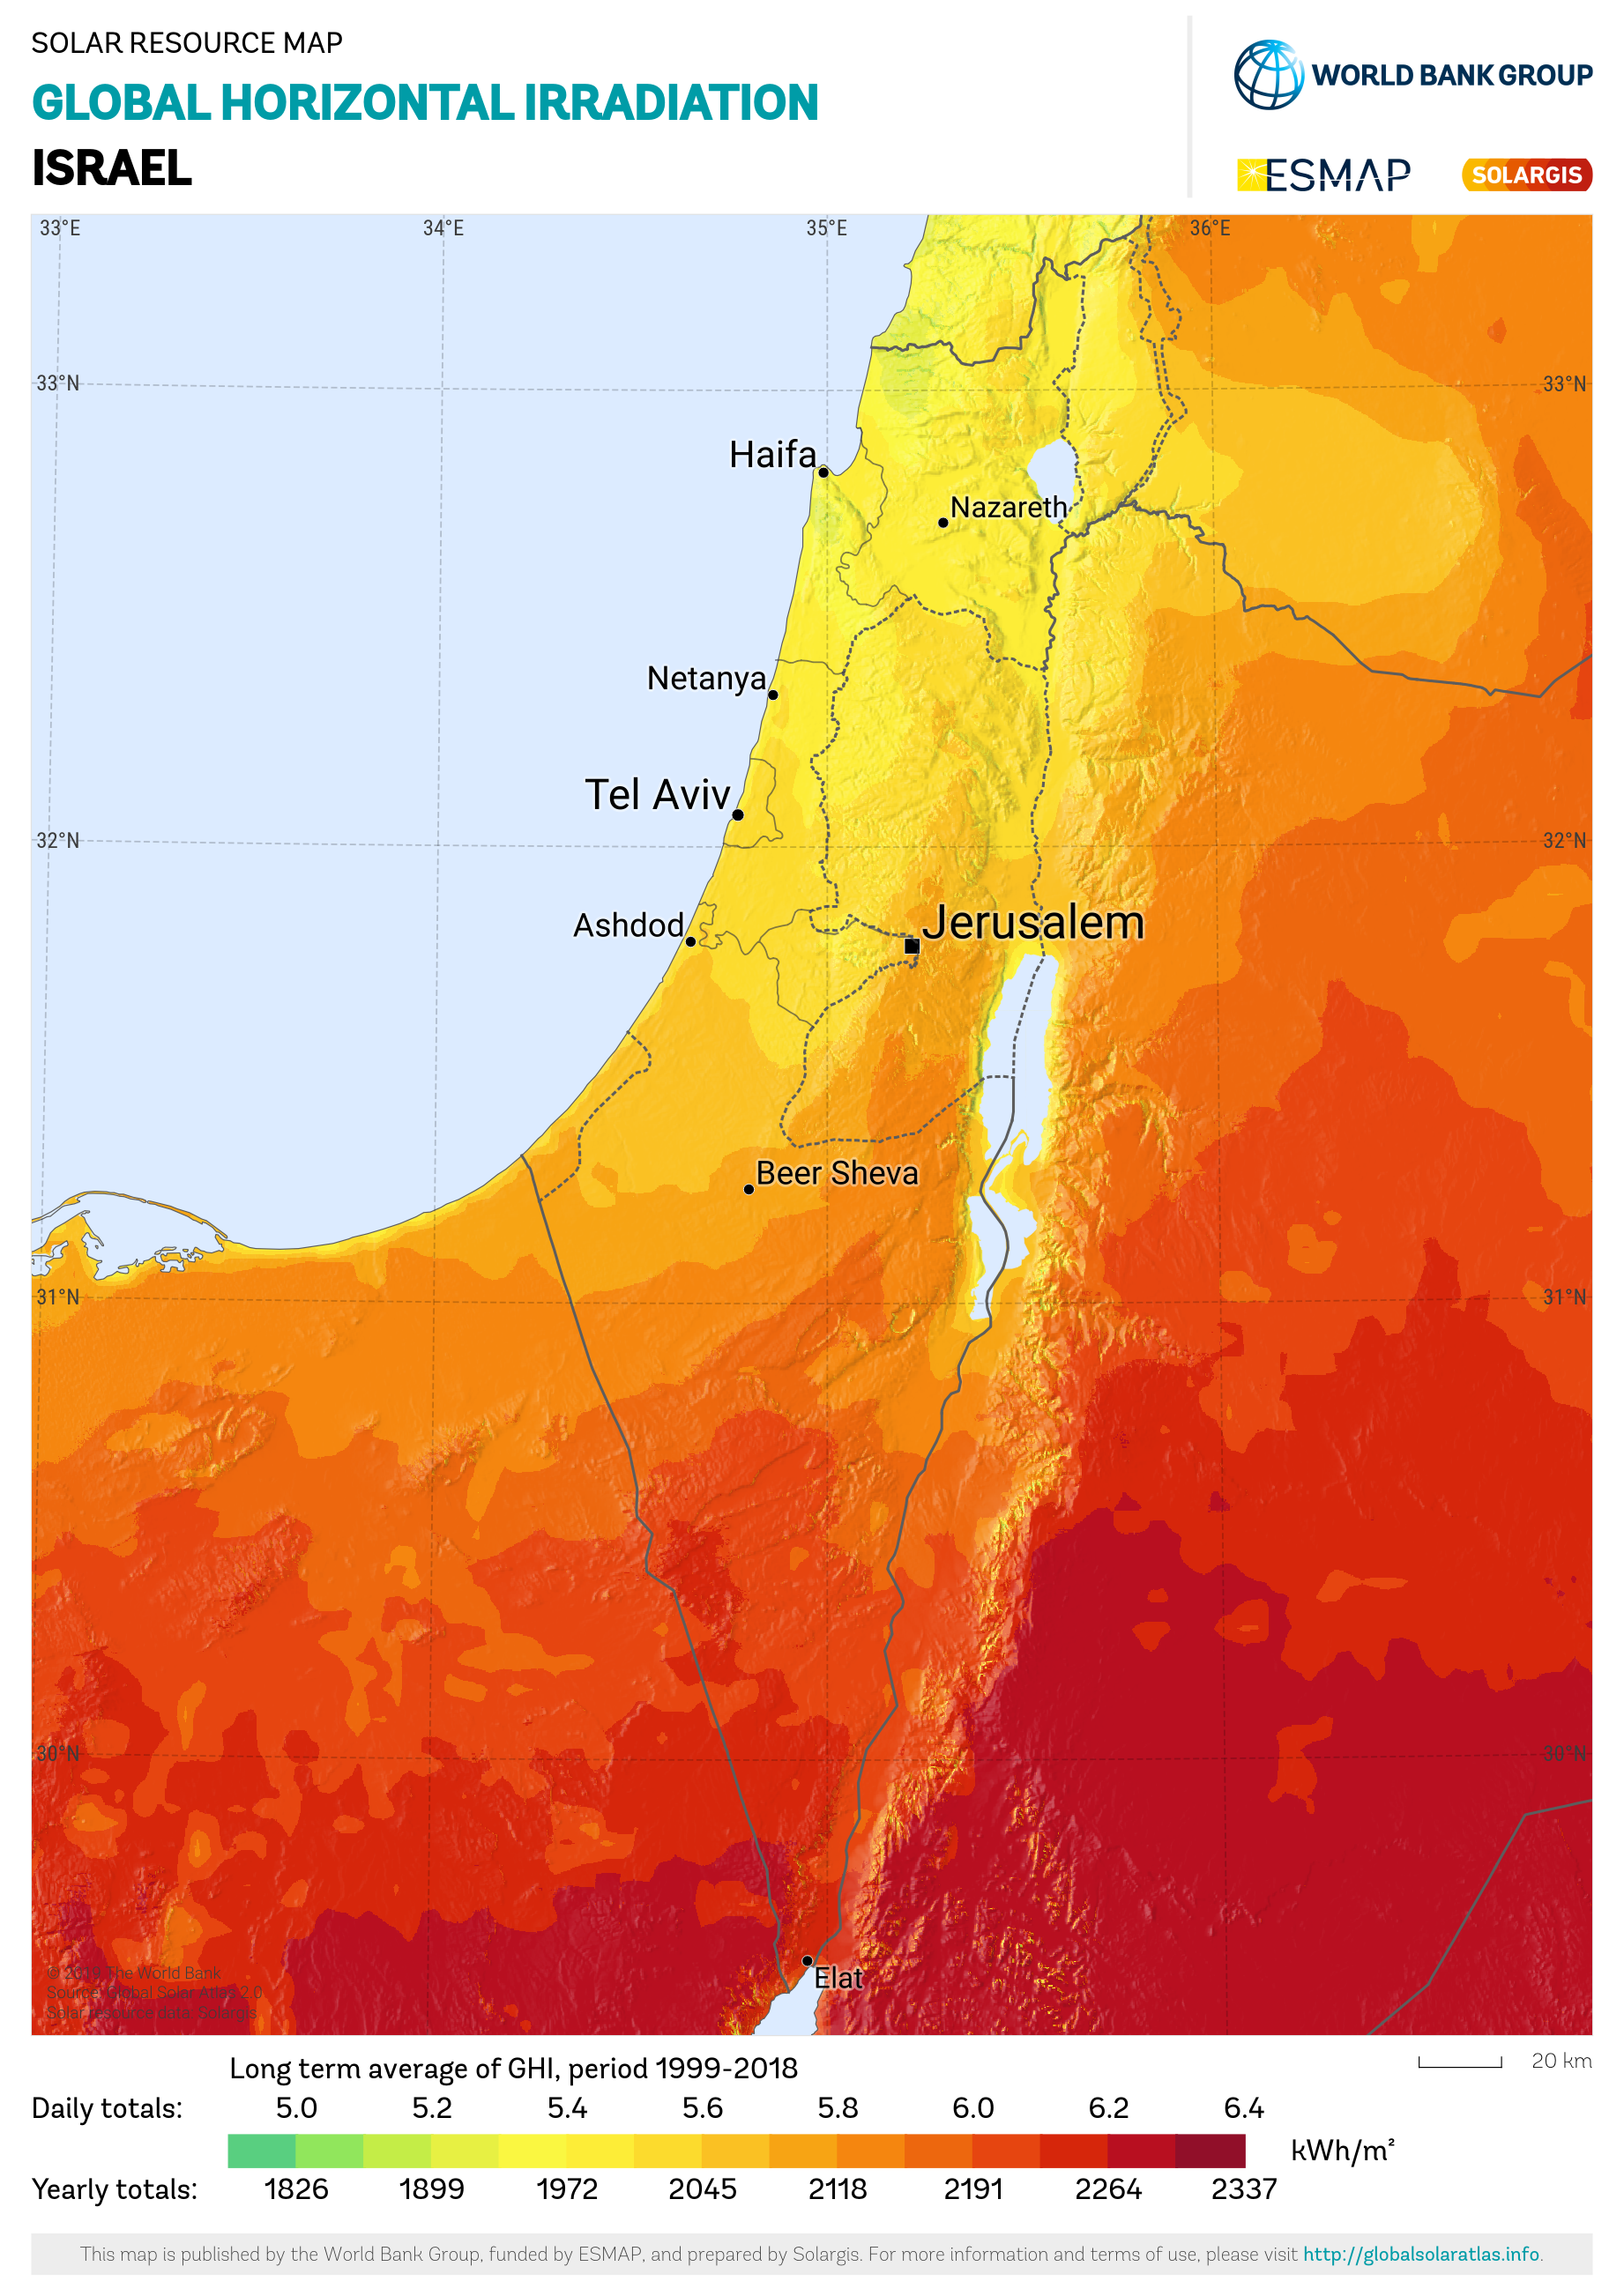
\includegraphics[width = \textwidth]{solar_maps/israel/israel_ghi}
  	\caption{Solar resource map of the long term average global horizontal irradiation of Israel. (Image credit: \cite{GlobalSolarAtlas:2020, Solargis:2021})}
	\label{fig:ghi_israel}
\end{figure}
\begin{figure}[h!]
	\centering
  	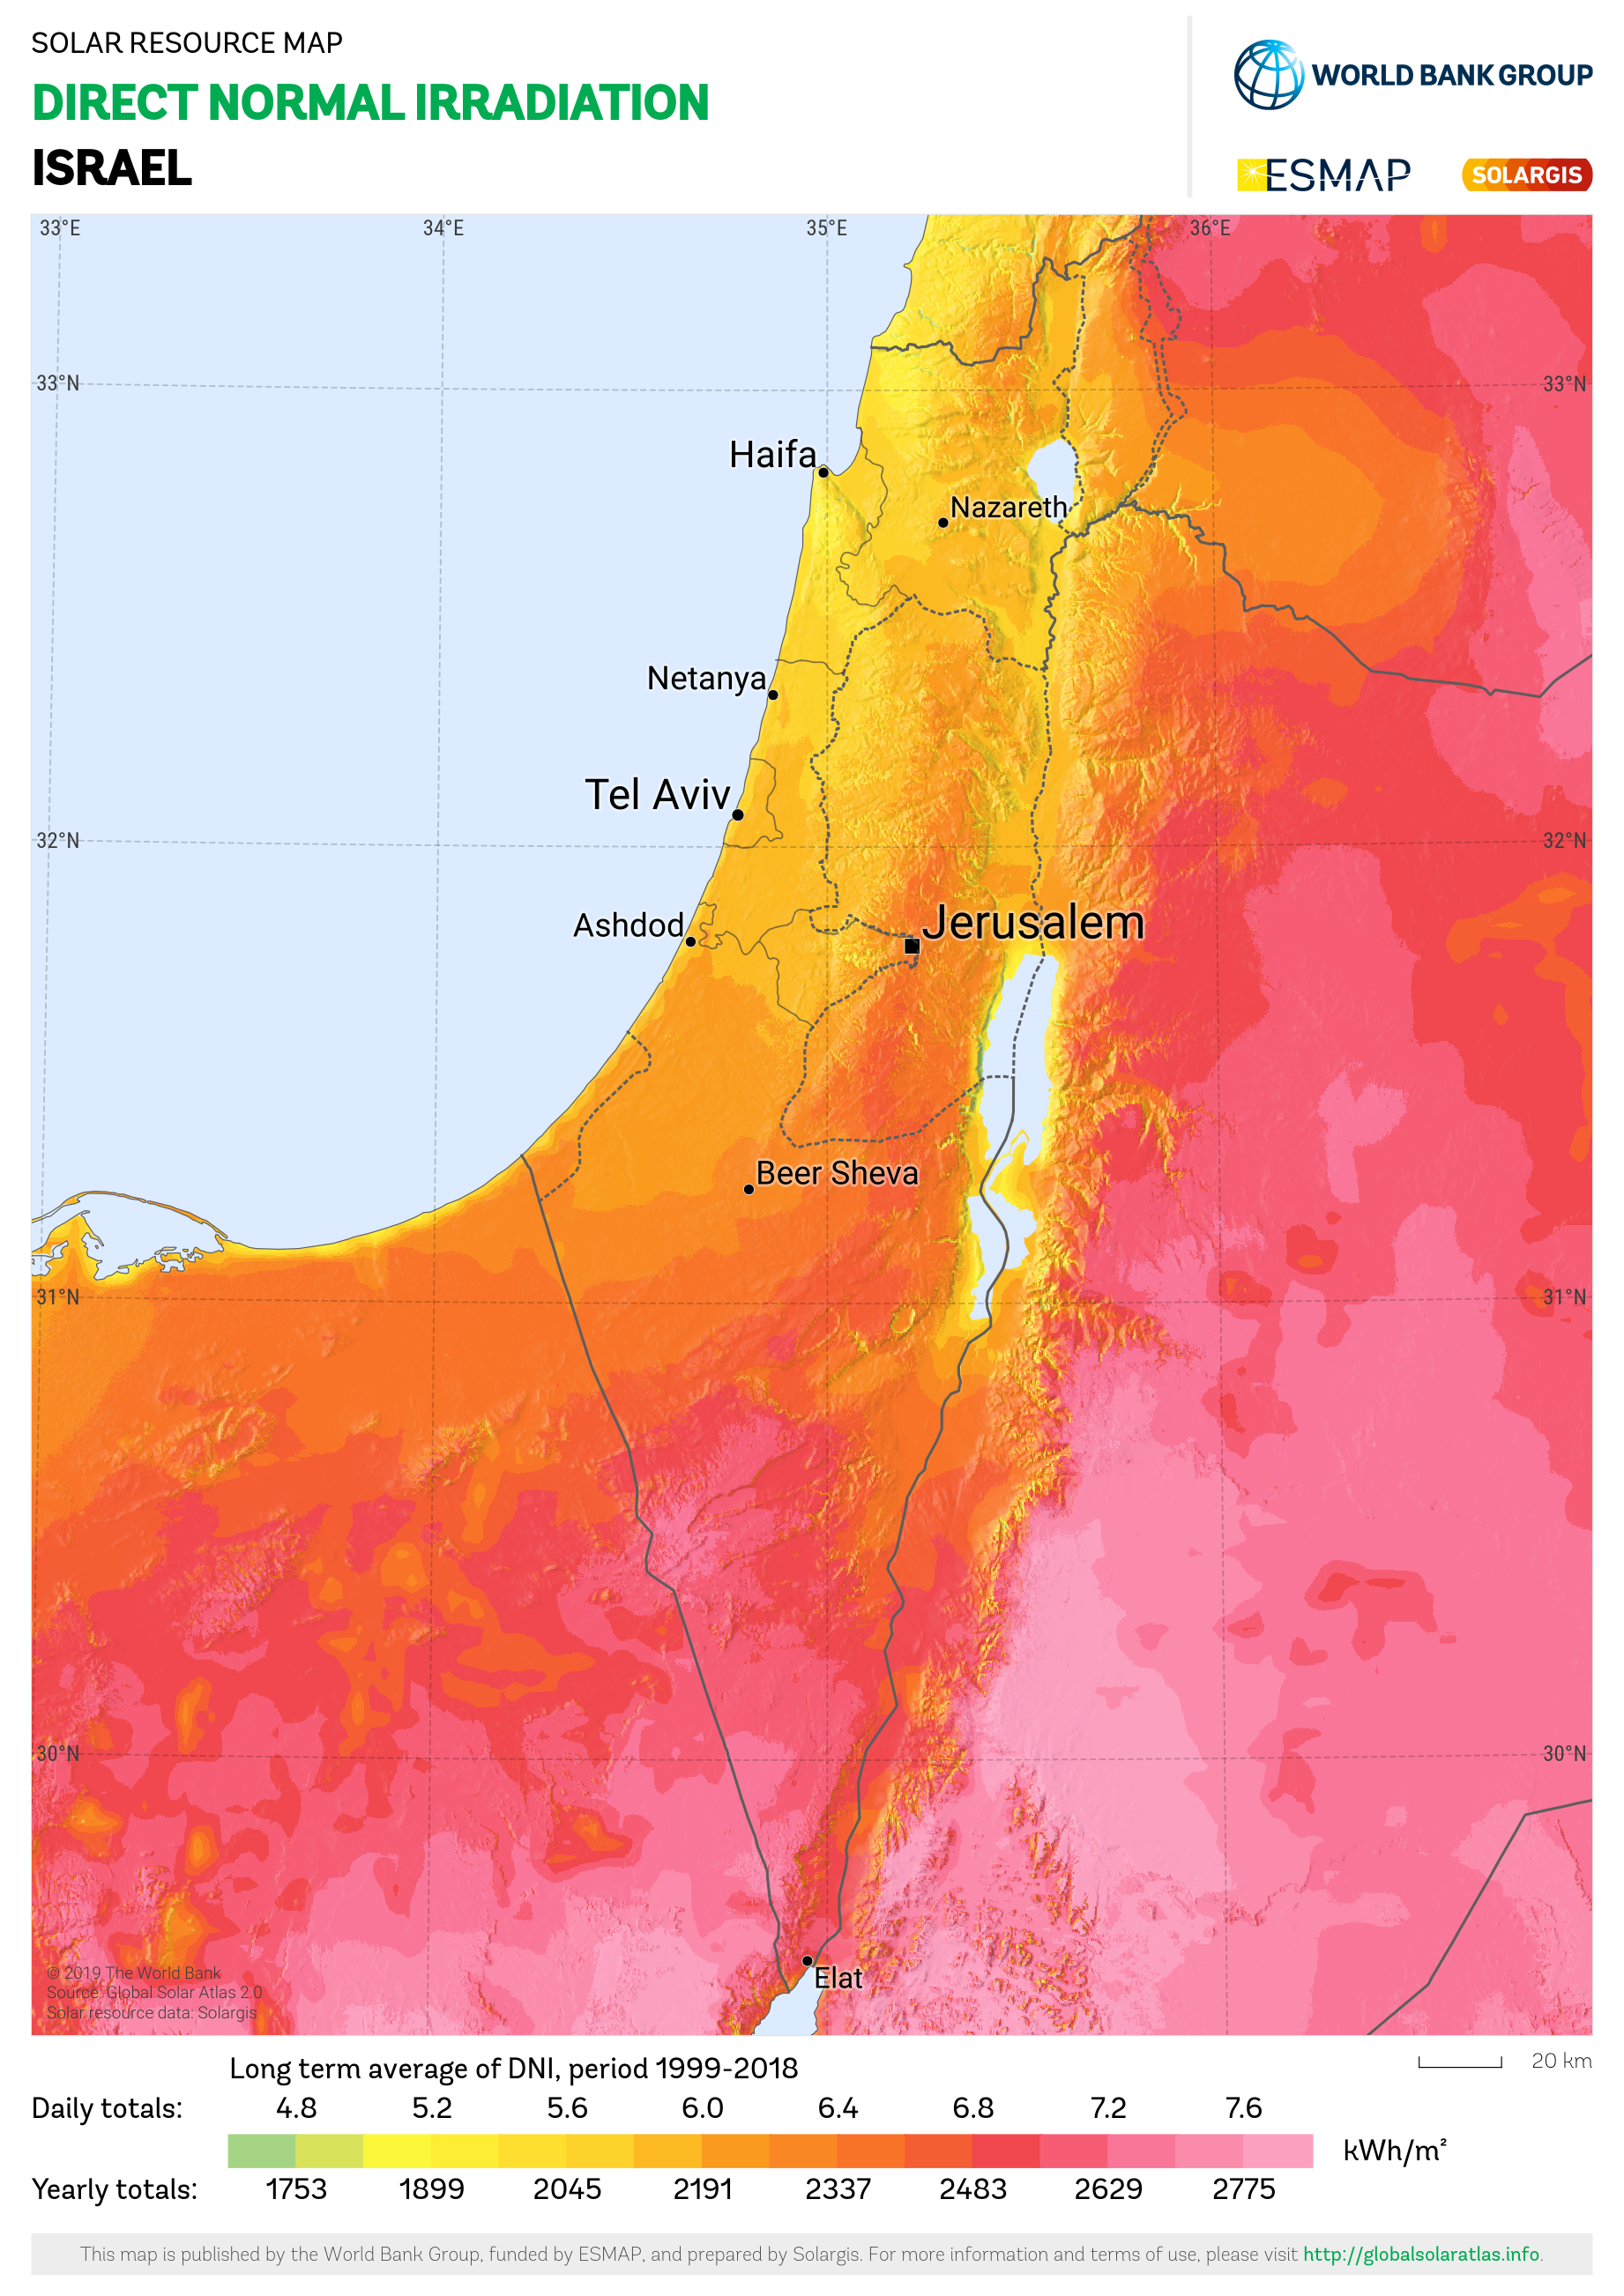
\includegraphics[width = \textwidth]{solar_maps/israel/israel_dni}
	\caption{Solar resource map of the long term average direct normal irradiation of Israel. (Image credit: \cite{GlobalSolarAtlas:2020, Solargis:2021})}
	\label{fig:dni_israel}
\end{figure}








% Warum wurde DAS Energy nicht verwendet!


% REFLECTION MAKE THE SIM BETTER AND MORE ACCURATE!!

 %OK
\chapter{Conclusion and critical reflection}
In addition to the summary and conclusion of the results, a critical examination of this thesis is presented in the following sections. 

\section{Conclusion}
In this section the findings and results of this thesis are summarized and concluded. First the results of the designed voice communication system are presented, followed by the self-sufficient energy distribution system and finally the usability of the system on Mars is discussed. 

\subsection{Voice communication system}
It was shown that a voice communication system can be designed according to requirements of the OeWF and that a performance estimation can be carried out on it. The designed voice communication system consists of a base station radio infrastructure, a radio system for the Serenity spacesuit simulator and a repeater radio infrastructure which is used to increase the covered mission area. It furthermore consists of handheld radios used by the the on-site support crew and the safety officers.

Both the Motorola Mototrbo DP 3601 handheld VHF radios and the existing frequency license for $158,950\mathrm{MHz}$, owned by the OeWF, were reused. In addition to the existing infrastructure, further Motorola Mototrbo radios were procured, with which an infrastructure was designed so that a theoretical mission area with a diameter of $15\mathrm{km}$ can be covered. 

The model for plane earth signal budget was calculated for two cases to show that the fade margins of the voice communication system do not fall below a minimum value of $20\mathrm{dB}$. In the first case it was assumed that all designed radio systems in the voice communication system were transmitting with maximum transmission power and the second case took into account the limitation of the transmission power to a maximum of $5\mathrm{W}$. In both cases the minimum fade margin resulted in $21,595\mathrm{dB}$.

With regard to the Serenity spacesuit simulator, a place for the Serenity radio system in the HUT of the spacesuit simulator was found in such a way that its antenna is installed vertically at a height of $1,65\mathrm{m}$ above the ground for a standard male AA, or at a height of $1,55\mathrm{m}$ above the ground for a standard female AA. The radio system is installed in such a way that it can be recharged in this position and removed if necessary. An approach with a wired PTT button and a wireless Bluetooth headset was chosen to reduce the cabling effort. This also has the advantage that an AA can put on the headset before donning and simply step into the spacesuit simulator. The same applies to doffing. 

The requirement for the operating temperature of the Serenity radio system could not be fully demonstrated. The data sheet of the radio device, the PTT button, the cables and the connections involved show that they meet this requirement. However, no specifications could be found for the Bluetooth headset and the audio jack that connects the PTT button to the radio device. No experiments were carried out either. In order to show that these components meet the temperature requirement, further experiments must be carried out. Alternatively, a Bluetooth headset was presented which fulfills this requirement and is compatible with the radio system. Furthermore, an audio jack that meets this requirement can be requested directly from Motorola Solutions inc. 

Since the W-LAN based voice communication system has not yet been fully developed, no qualitative statement can be made regarding the requirement for the combined mass of the two radio systems. Their combined mass is currently $853,33\mathrm{g}$ with the proposed Bluetooth headset and $866,33\mathrm{g}$ with an alternative Bluetooth headset.  

\subsection{Self-sufficient energy distribution system}
Because the repeater radio system cannot be recharged as easy due to its remote location in the field, an environmentally friendly self-sufficient energy distribution system was designed to supply it with electrical energy. In general it consists of one ore more PV generators connected in parallel, a solar charging controller and a $\mathrm{LiFePO}_4$ battery. A \MATLAB simulation was developed which provides an estimation of wether the self-sufficent energy distribution system can supply the repeater radio infrastructure with enough electrical energy at a given mission location or not. This simulation is based on models of the angular relationships between the Sun and Earth, photovoltaic generators and $\mathrm{LiFePO}_4$ batteries. To obtain a model from the latter, discharging and charging experiments were carried out.

\MATLAB simulations of the self-sufficient energy distribution system for the upcoming analog Mars field mission AMADEE-20 in October 2021 in the Negev Desert in Israel showed that the repeater radio system can be sufficiently supplied with electrical energy from one PV generator. Similar results could be obtained for Vienna, Austria, in April 2021. It was shown, however, that at least two PV generators in parallel are required.

\subsection{Martian application}
When examining the self-sufficient energy distribution system, two components of the system emerged which required special attention. First, the PV generator, as it requires a larger energy converting area due to the lower solar radiation on Mars, and second, the $\mathrm{LiFePO}_4$ battery due to its temperature dependece. An equation was derived which compares the area ratio between a PV generator on Earth and one on Mars. However, this should only be used as a rough estimation, since the temperature dependence of said generator on the surface of Mars has to be investigated more closely. Taking into account dust storms, it was found that during such storms, due to the diffuse component of sunlight, still enough electrical energy can be converted. However, dust that accumulates on the PV generator's energy converting area can become a problem in the long term. Regarding $\mathrm{LiFePO}_4$ batteries, it was found that these have a high temperature dependence and therefore have to be heated or cooled accordingly. For this, a higher energy consumption must be planned.

After examining the voice communication system, it was found that the temperature of the radio devices and components has an influence on their thermal noise. Similar to the self-sufficient energy system, the temperature dependence also needs to be examined in more detail here. So that a reliable voice communication system can be set up on the surface of Mars, it is advisable to carry out a more detailed investigation of the multipath propagation of the electromagnetic waves, so that the infrastructure can be optimally placed. During the day, the Martian ionosphere can be used as a reflector for global communication for frequencies in the VHF range. At night, however, this effect is limited because Mars has almost no intrinsic magnetic field. This effect therefore depends heavily on the time of the day. It is assumed that the Martian troposphere has no influence on the propagation of electromagnetic waves, as it is very thin. The impact of dust storms needs further investigation. However, it is assumed that the signal attenuation for the VHF band is rather low. Finally, sufficient redundancy must be ensured so that a failure of the voice communication system is very unlikely, as this can become dangerous for astronauts. 


\section{Critical refelction}
A critical reflection of this thesis is now presented to point out the areas in which further studies need to be carried out. First the voice commuication system will be examined and then the self-sufficient energy distribution system.

\subsection{Voice communication system}
As already mentioned, a number of factors that influence the performance of the designed voice communication system were neglected. In the literature \cite{Glover:2010} it is explained that special consideration should be given to the temperature of the individual radio devices and components in order to investigate their thermal noise. Independent of this noise source, this literature also deals with other noise sources that could have an influence on the system. Furthermore, a more detailed examination of the signal budget should be carried out in order to take into account possible obstacles in the path of the electromagnetic waves. This includes, for instance, ground roughness. The basis for this can be found in books \cite{Parsons:2000, Mecklenbrauker:2017}. For a Martian application this topic is covered in the NASA publication \cite{Ho:2002}. Subsequently, a simulation with topological maps for different mission locations can be carried out. Finally, the influence of the Earth's atmosphere on the propagation of electromagnetic waves should be taken into account \cite{Glover:2010, Parsons:2000}. In order to obtain empirical data to get a better model of the voice communication system for simulations, experiments need to be carried out with the assembled voice communication system in different locations \cite{LinkMargin:2016}. 

\subsection{Self-sufficient energy distribution system}
Instead of the approximated equations for the angular relationships between the Sun and Earth, databases can be used which contain measured values of these angles throughout the year. Thus, the accuracy of the \MATLAB simulation can be improved. In addition, instead of the Gaussian fitting function -- which was used to simulate the radiation flux $\Phi_\mathrm{G}$ -- a more precise curve shape as shown in \cite{Babikir:2020} can be used. 

Regarding the PV generator, the \emph{two diodes model} can be used to improve the accuracy of the \MATLAB simulation as well. This model is much more accurate because it takes into account the parallel resistance, the series resistance and the leakage currents of a PV cell. However, in order to obtain the necessary parameters for this model, various experiments must be carried out on a PV generator \cite{Mertens:2015, Wagner:2018}. Furthermore, the effect of shade on the PV generator's energy converting area must be investigated, as well as its power output for different weather conditions \cite{Mertens:2015}.

To further increase the accuracy of the \MATLAB simulation, a temperature model \cite{Hausmann:2013, Ala-A.-Hussein:2015, Chin:2018}, a capacity fading model \cite{Li:2018} and the transient (dynamic) behavior, which is described by the Thevenin model \cite{He:2011, Rahmoun:2012, Hentunen:2014, Li:2018, Hinz:2019, Hossain:2019, Saldana:2019}, of the $\mathrm{LiFePO}_4$ battery should be considered.

Finally, the \MATLAB simulation can be sped up by reducing the amount of \codeword{for} loops and by removing possible bugs. Improvements of its accuracy can also be achieved by implementing the described step function of the load current and the charging behavior of the $\mathrm{LiFePO}_4$ battery. 


\clearpage
\pagenumbering{arabic}	% resets page numbering to 1
\renewcommand*{\thepage}{A\arabic{page}}
\appendix

\fancyhead{}																% clearing all the head fields
\fancyhead[RE]{Voice communication system for a spacesuit simulator}		% RO ... Right Odd, LE ... Left Even
\fancyhead[LO]{\nouppercase{\leftmark}}										% also try \rightmark, \leftmark and \chaptermark
\fancyfoot{}
\fancyfoot[RE, LO]{\thepage}

% Sort:
\chapter{Austrian Space Forum} \label{ap:oewf}
Since 1999, the Austrian Space Forum continuously motivates dedicated space pioneers to participate in humanities mission to explore the vast universe and fuels their passion for adventure and exploration. A quotation which is written on a wall in the OeWF Suit-laboratory in Innsbruck, Austria, wonderfully depaints what this means and what the OeWF stands for:

\begin{displayquote}
\textit{``I am the power that proudly looks beyond the horizon, surpassing limits and expectations.\\\\ Honoring Europe's tradition of exploration with a new glow, I am the extraordinary union of engineering excellence, scientific curiosity and the people's passion for seeking new worlds, with every step carefully drafted with diligence, emotion and elegant design.\\\\ I am the magnet that attracts talent and hearts; the maker that symbolizes Europe's ambition to set sail for the unknown.\\\\ More than just a mission in time, I define missions for generations to come.\\\\ I am the Austrian Space Forum.''}
\end{displayquote}

\section{History}
As part of the PolAres program, which originated in 2007 after an international collaboration, the first spacesuit simulator called Aouda was developed. Its goal is to help humanity gain more knowledge and experience for future Mars missions by conducting simulations on Earth \cite{OeWF:2019_history}. Such simulations are possible because certain regions on Earth, like the Atacama Desert in South America, the Mojave Desert in North America, the Qaidam Basin in the Tibetan Plateau or the Turpan Desert in China, have at least one feature that resembles a Martian environment \cite{Salas:2011, Preston:2012, Preston:2014}. Due to this analogy, these regions are often referred to as analog Martian environments. Astronauts that conduct missions in these areas are refferd to as ananlog astronauts. As an example, figure \ref{fig:analogy_mars_oman} shows the geological Mars analogy between the elongated crater ``Spirit of St. Louis'' on Mars (figure \ref{fig:image_mars_elongated_crater}) and the Dhofar Desert in Oman (figure \ref{fig:image_oewf_oman}) \cite{Greicius:2015}. Areas like these provide a great opportunity for scientist, engineers and analog astronauts to study possible Martian environments. 
\vfill
\begin{figure}[h!]
	\centering
	\begin{subfigure}[b]{0.96\textwidth}	% 0.96
		\centering
		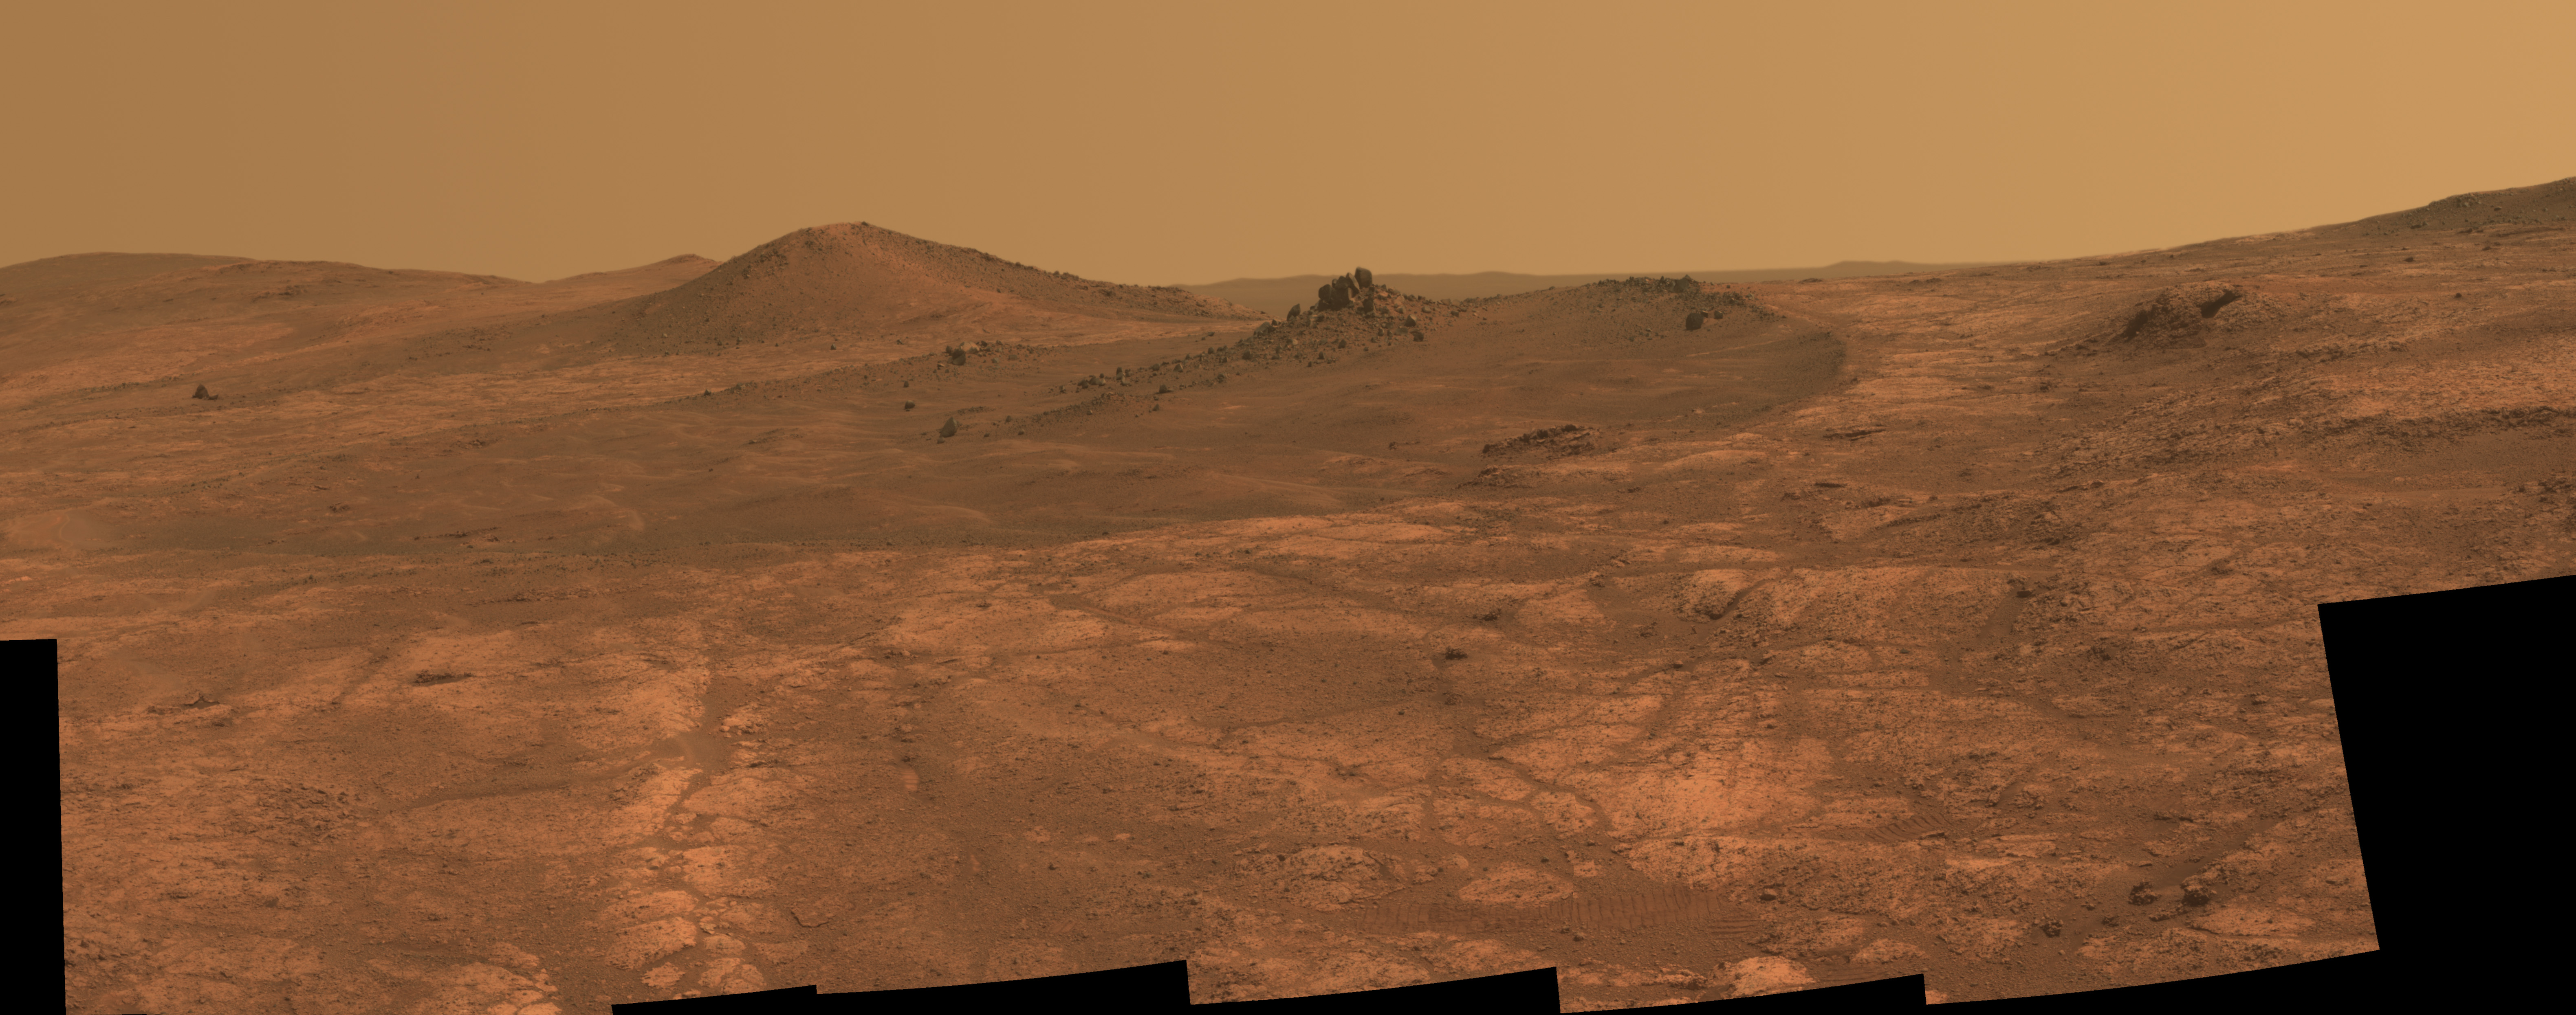
\includegraphics[width = \textwidth]{image_mars_elongated_crater}
		\caption{Elongated crater ``Spirit of St. Louis'' on Mars taken from the panoramic camera on NASA's Mars Exploration Rover Opportunity. (Image credit: \cite{Greicius:2015})}
		\label{fig:image_mars_elongated_crater}
	\end{subfigure}
	
	\hfill
	
	\begin{subfigure}[b]{0.96\textwidth}	%0.96
		\centering
		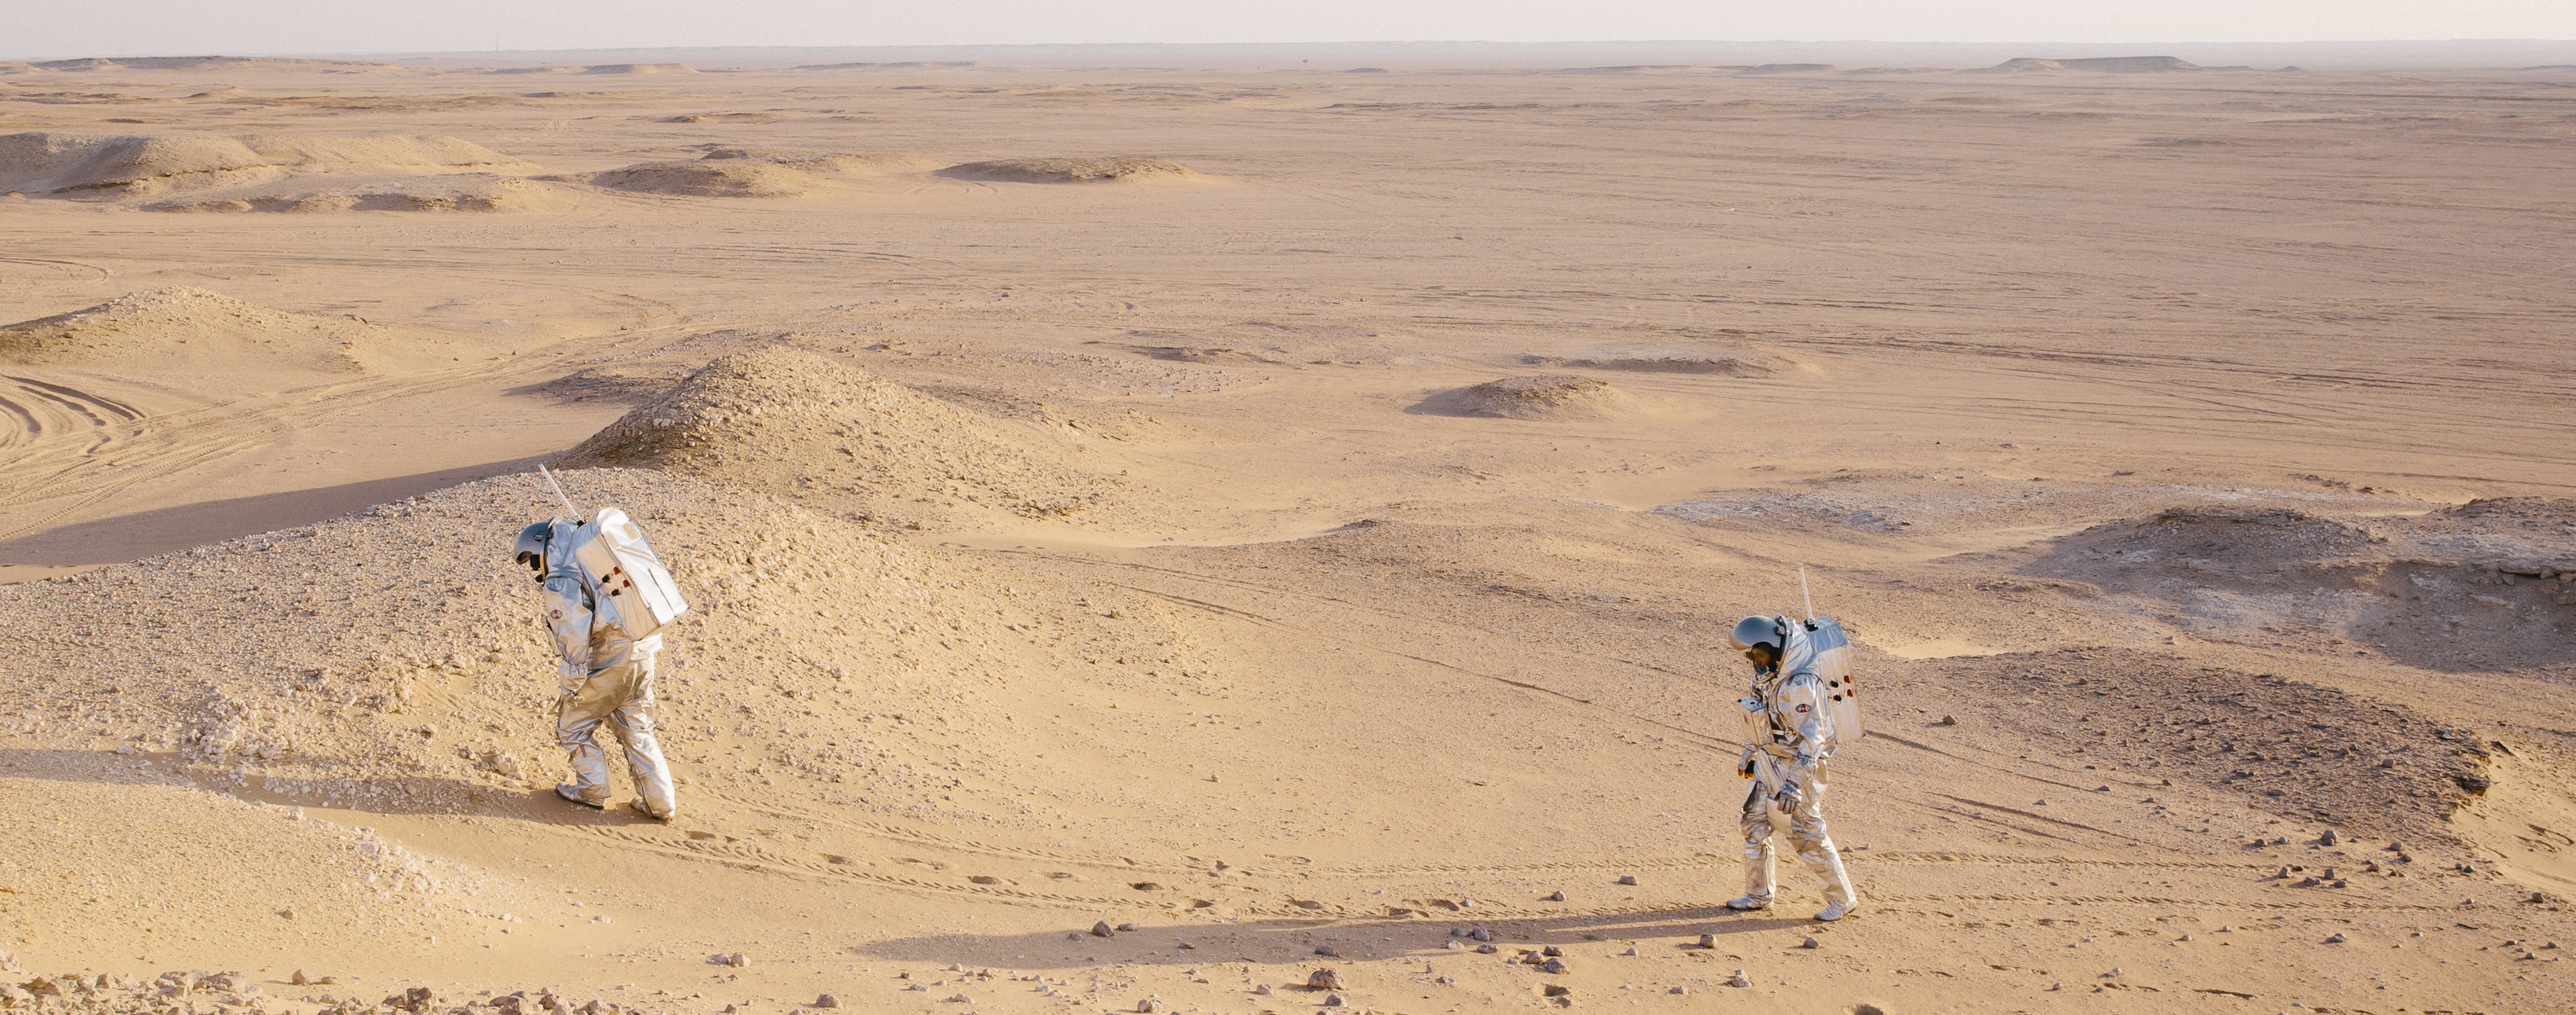
\includegraphics[width = \textwidth]{image_oewf_oman}
		\caption{Two analog astronauts from the OeWF performing a simulation with Aouda spacesuit simulators in the Dhofar Desert in Oman. (Image credit: OeWF/Florian Voggeneder)}
		\label{fig:image_oewf_oman}
	\end{subfigure}
	\caption{Visible geological similarities between the Martian surface and an analog Martian environment on Earth.}
	\label{fig:analogy_mars_oman}
\end{figure}
\vfill

With the help of Aouda, analog astronauts can conduct basic training, experiments and other important tasks while experiencing similar restrictions and technical aids a Mars spacesuit in two to three decades will have. This makes it possible to collect vital data from different scientific areas, which can help future astronauts to safely prepare for Mars missions \cite{OeWF:2019_history}.

In 2010, the Aouda spacesuit simulator was tested for the first time in a field simulation on a glacier in the Kaunertal in Austria. The mission lasted for two days and aimed to perform astrobiological experiments. Further missions took place in 2011 in Rio Tinto in Spain, in 2012 on the Dachstein mountains in Austria, in 2013 in the northern Sahara near Erfoud in Morocco (MARS2013), in 2015 again in the Kaunertal in Austria (AMADEE-15) and in 2018 in the Dhofar Desert in Oman (AMADEE-18). The next mission, called AMADEE-20, was planned to take place in late 2020 in the Negev Desert in Israel but it was postponed until October 2021 due to the ongoing SARS-CoV-2 pandemic. Missions carried out by the OeWF generally last from a couple of days to a few months \cite{OeWF:2019_missions, Israel:2020}.

\section{Serenity spacesuit simulator}
After ten years and more than 750 hours of \emph{extravehicular activities} (EVAs), Aouda's successor is the Serenity spacesuit simulator. In participation with national and international high-end universities and companies, Serenity has been under development since 2018. Bernhard Kaliauer Design Studio's first concept of Serenity is shown in figure the \ref{fig:serenity_design_study}.
\begin{figure}[h!]
	\centering
	\begin{subfigure}[b]{0.47\textwidth}
		\centering
		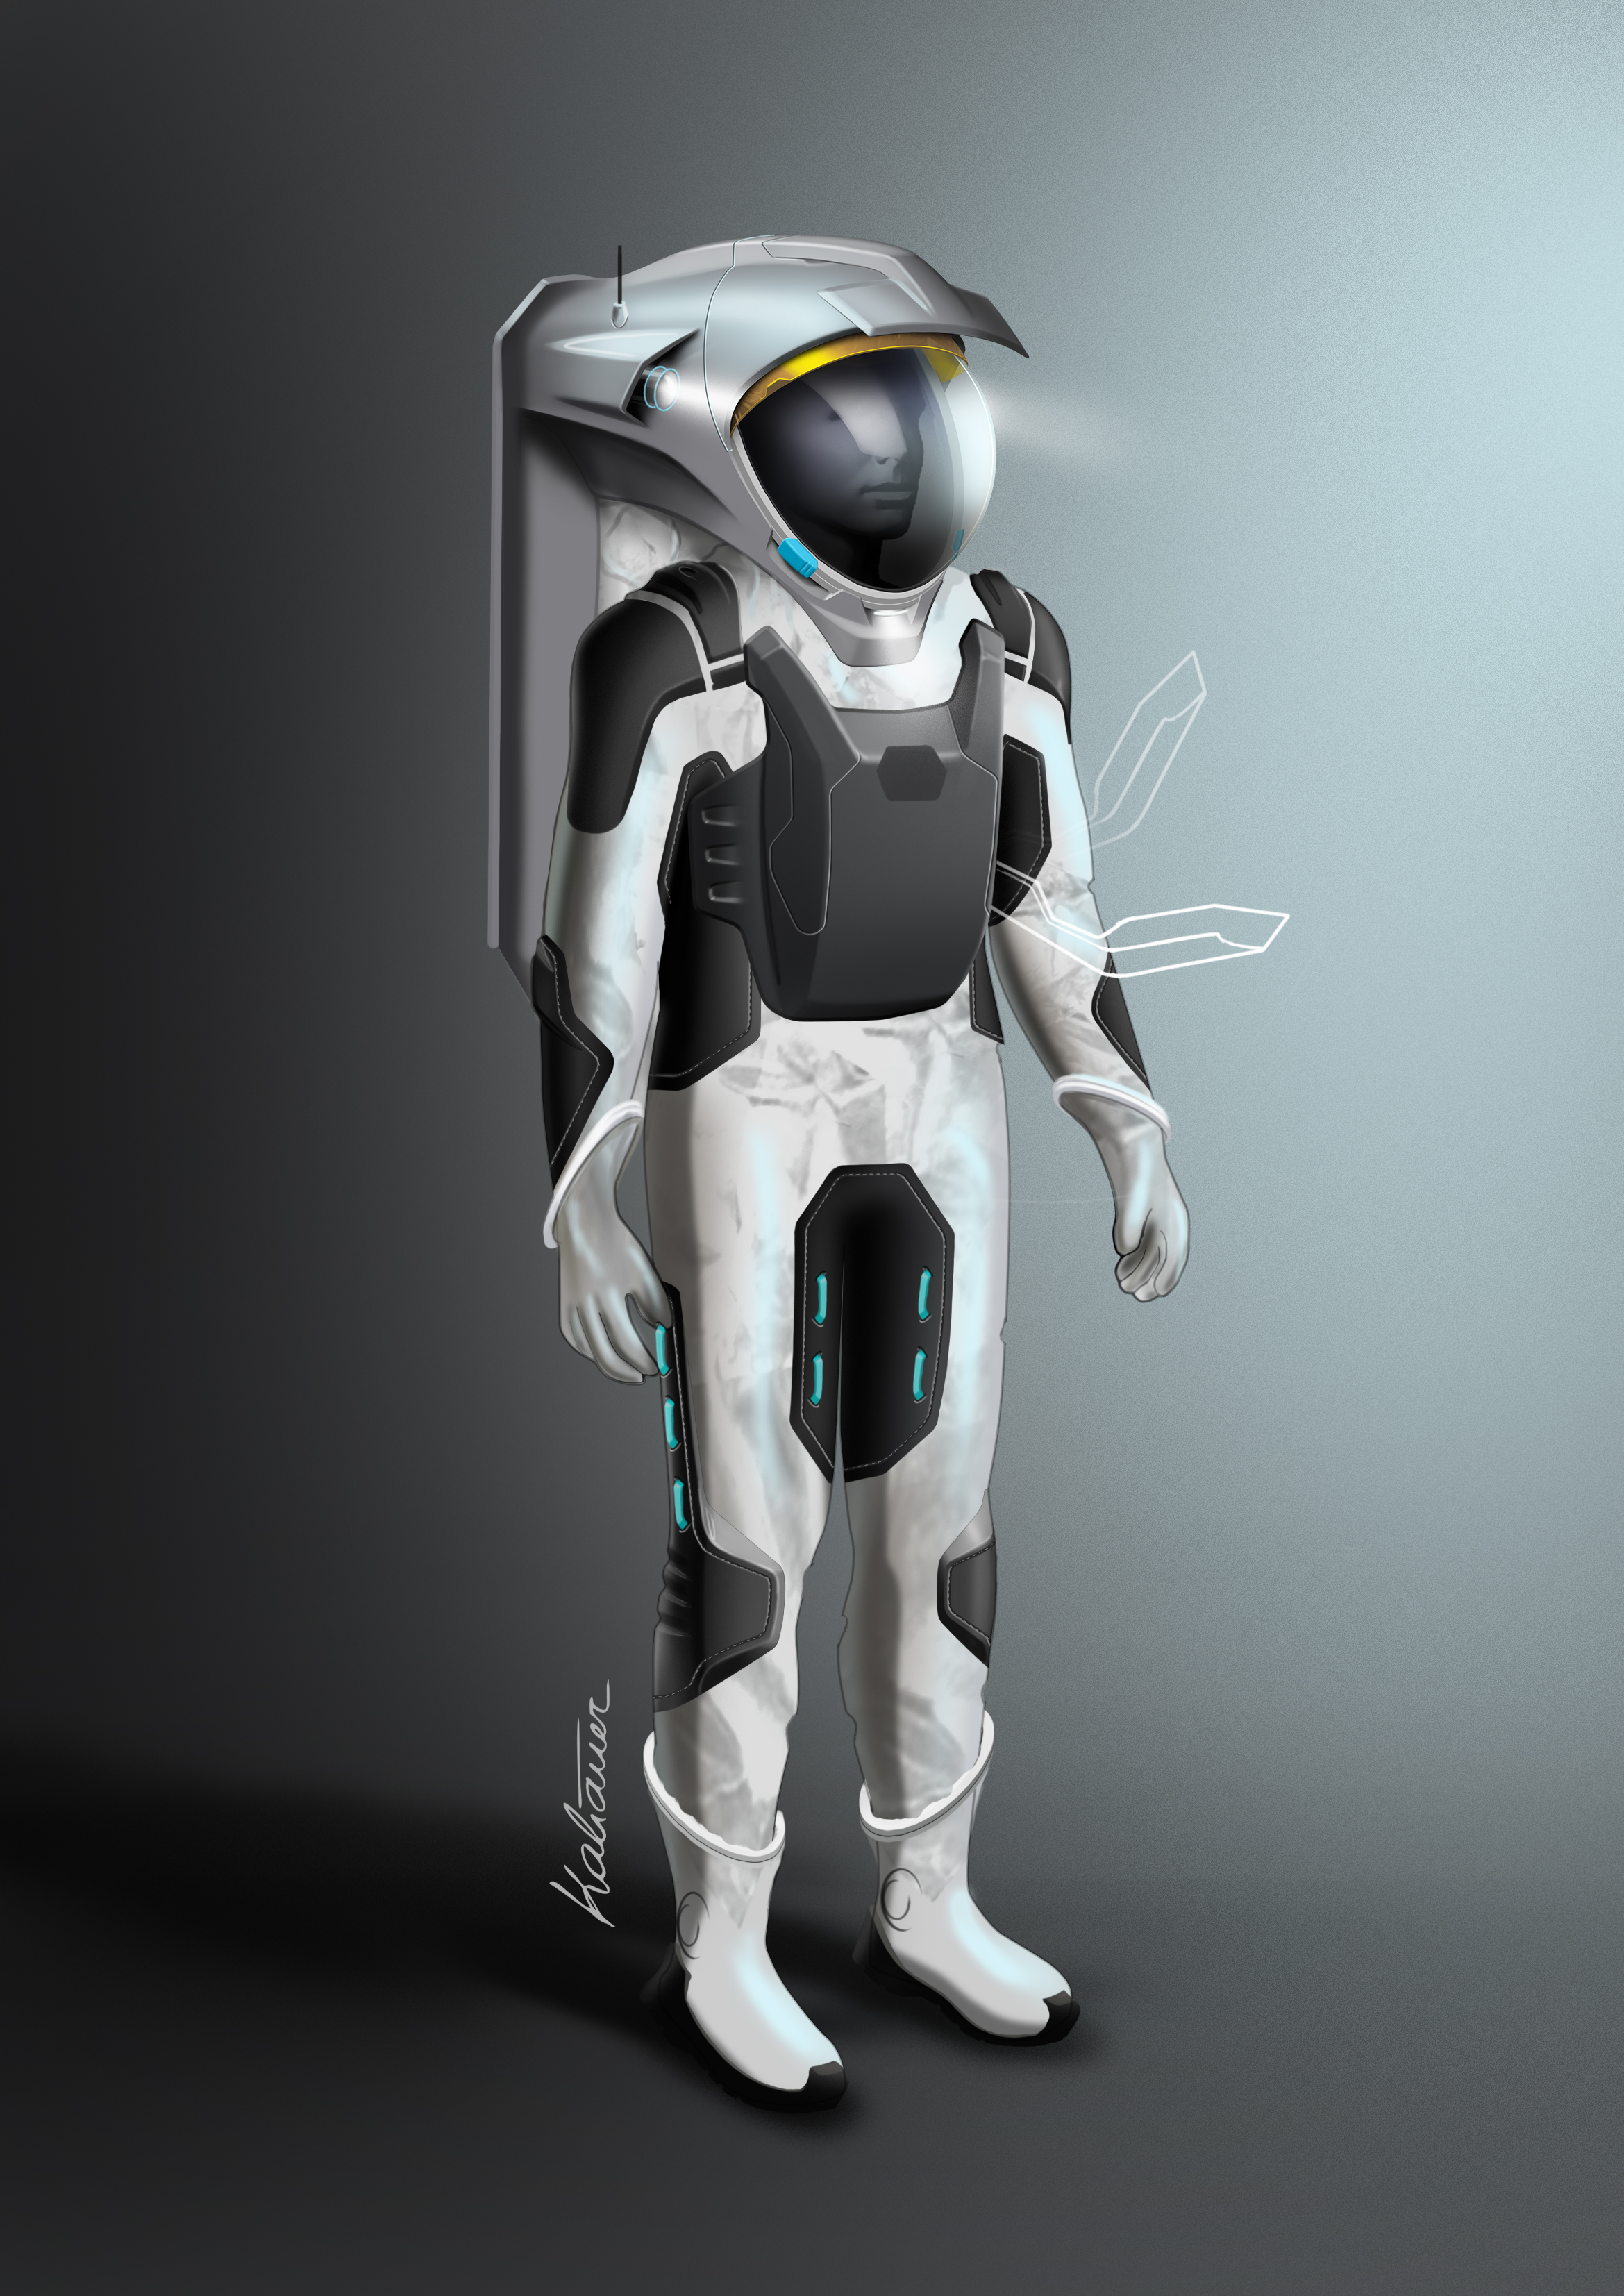
\includegraphics[width = \textwidth]{image_serenity_front_view}
		\caption{Front view}
		\label{fig:image_serenity_front_view}
	\end{subfigure}
	\hspace{5pt}%
	\begin{subfigure}[b]{0.47\textwidth}
		\centering
		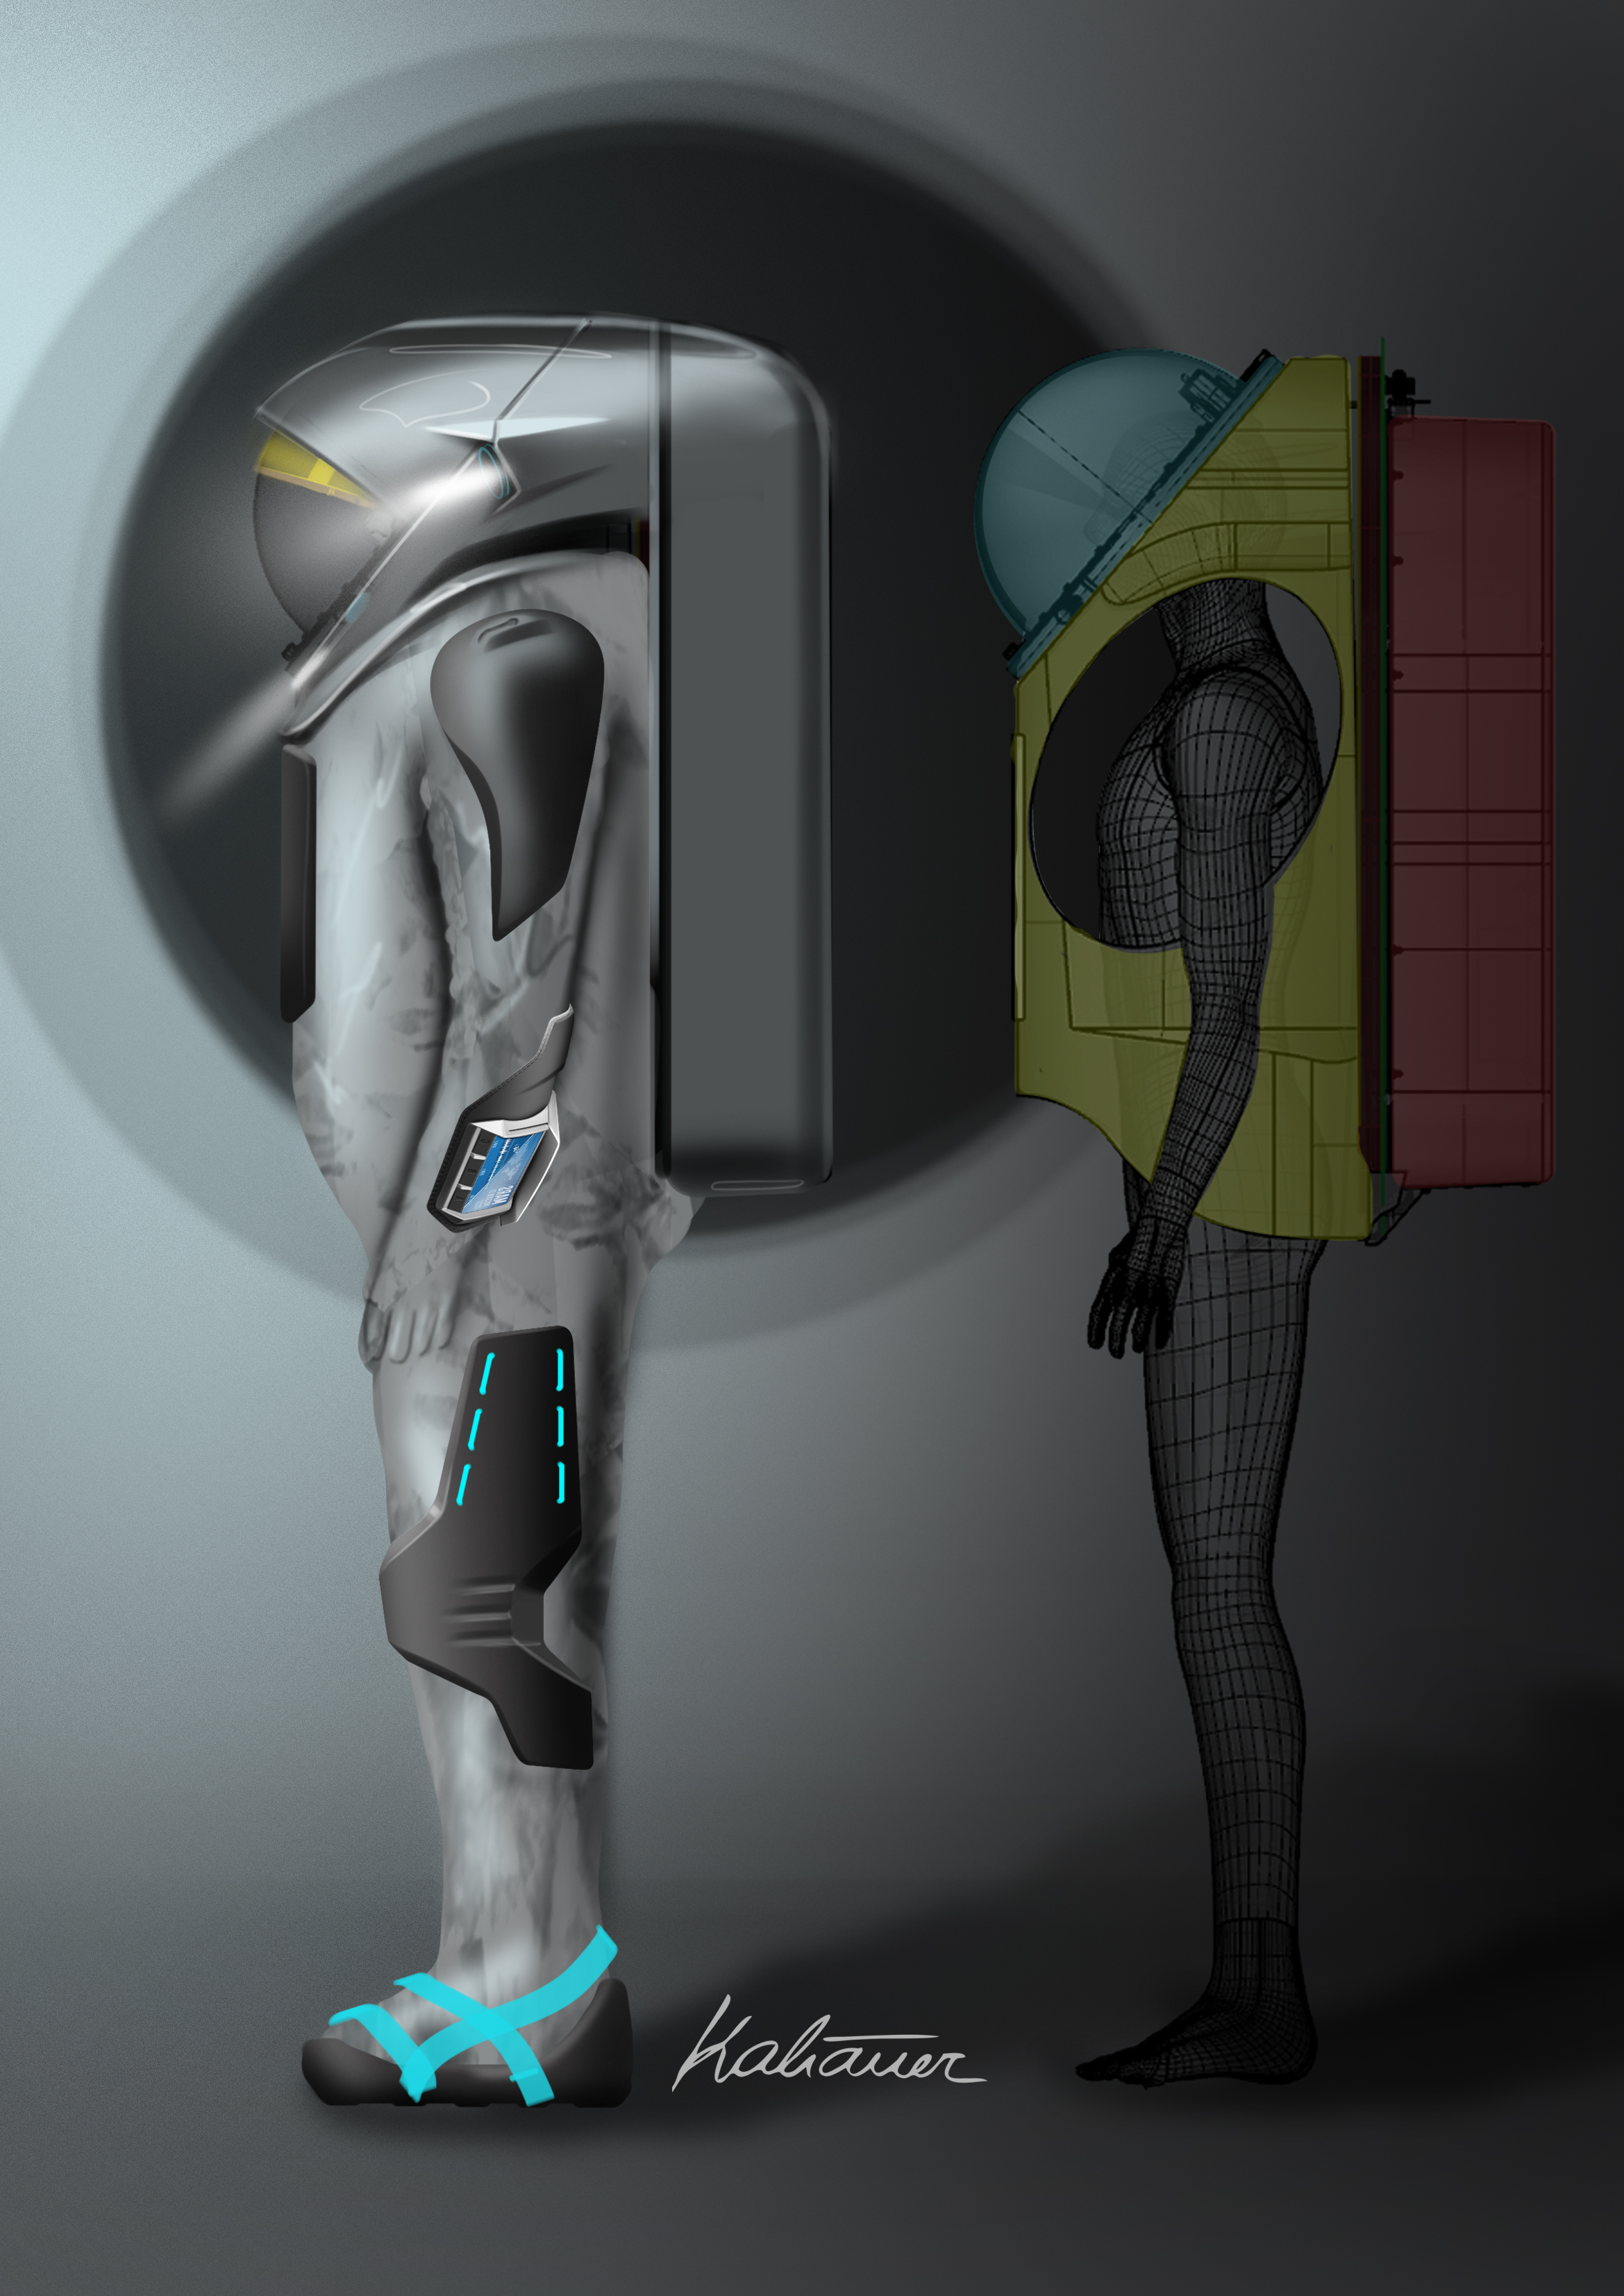
\includegraphics[width = \textwidth]{image_serenity_side_view}
		\caption{Side view}
		\label{fig:image_serenity_side_view}
	\end{subfigure}
	\caption{Serenity spacesuit simulator design study. (Image credit: OeWF/Bernhard Kaliauer Design Studio)}
	\label{fig:serenity_design_study}
\end{figure}

It is important to the OeWF to make the transition from Aouda to Serenity as fluid and environmentally friendly as possible. That is why, on the one hand, tried and tested materials are being upgraded and re-used, which shortens the retraining time of the analog astronauts, and on the other hand, a number of innovations are introduced based on the knowledge gathered over the past few years. 

Apart from the complete revision to carry out even more realistic simulations, a new advanced rear-entry system will be implemented. This system represents the latest NASA standard for Mars missions due to its ability to easily dock at a habitat, thus reducing contamination and donning time \cite{EVA:2018}.


\chapter{Mathematical basics}
This appendix covers the most important mathematical basics that were used. More information can be found in the books \cite{Schwarz:2011, Rudolf:2014, Taschner:2014, Taschner:2015, Kugi:2021}.

\section{Integral of the Gaussian bell curve} \label{sec:gauss_general}
The shifted Gaussian bell function, shown in the figure \ref{fig:tikz_gauss_curve_general}, is used to model the solar energy curve (see subsection \ref{sec:solar_energy_curve}). Therefore, the mathematical approach of calculating the area of the Gaussian bell function -- enclosed by the curve and the x-axis -- will be explained.
\begin{figure}[h!]
	\centering
	
\tikzset{every picture/.style={line width=0.75pt}} %set default line width to 0.75pt        

\begin{tikzpicture}[x=0.75pt,y=0.75pt,yscale=-1,xscale=1]
%uncomment if require: \path (0,300); %set diagram left start at 0, and has height of 300

%Image [id:dp36698085633645405] 
\draw (328.75,179) node  {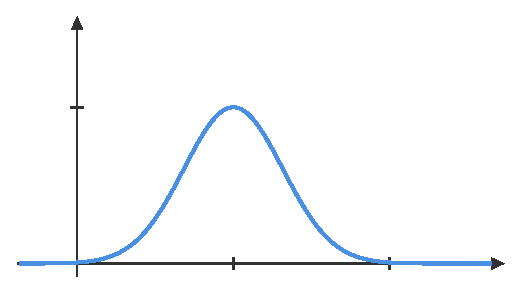
\includegraphics[width=233.63pt,height=124.5pt]{images/image_shifted_gauss_curve}};
%Straight Lines [id:da37857254246955074] 
\draw [color={rgb, 255:red, 155; green, 155; blue, 155 }  ,draw opacity=1 ] [dash pattern={on 4.5pt off 4.5pt}]  (222,153.7) -- (303.4,153.7) ;
%Straight Lines [id:da32947142925776296] 
\draw [color={rgb, 255:red, 155; green, 155; blue, 155 }  ,draw opacity=1 ] [dash pattern={on 4.5pt off 4.5pt}]  (311.4,243) -- (311.4,155.7) ;
%Shape: Circle [id:dp5744124003855682] 
\draw  [fill={rgb, 255:red, 255; green, 255; blue, 255 }  ,fill opacity=1 ] (309.4,153.7) .. controls (309.4,152.6) and (310.3,151.7) .. (311.4,151.7) .. controls (312.5,151.7) and (313.4,152.6) .. (313.4,153.7) .. controls (313.4,154.8) and (312.5,155.7) .. (311.4,155.7) .. controls (310.3,155.7) and (309.4,154.8) .. (309.4,153.7) -- cycle ;

% Text Node
\draw (202.5,76.9) node [anchor=north west][inner sep=0.75pt]  [font=\footnotesize]  {$f( x)$};
% Text Node
\draw (488,248.4) node [anchor=north west][inner sep=0.75pt]  [font=\footnotesize]  {$x$};
% Text Node
\draw (305,262.9) node [anchor=north west][inner sep=0.75pt]  [font=\footnotesize]  {$x_{0}$};
% Text Node
\draw (397.5,259.4) node [anchor=north west][inner sep=0.75pt]  [font=\footnotesize]  {$2x_{0}$};
% Text Node
\draw (197,256.4) node [anchor=north west][inner sep=0.75pt]  [font=\footnotesize]  {$0$};
% Text Node
\draw (191,147.4) node [anchor=north west][inner sep=0.75pt]  [font=\footnotesize]  {$C$};


\end{tikzpicture}


	\caption{Shifted Gauss bell.}
	\label{fig:tikz_gauss_curve_general}
\end{figure}

In general, the Gaussian bell function can be written as shown in the equation (\ref{eq:gauss_curve}), with its corresponding indefinite Integral shown in the equation (\ref{eq:integral_gauss}).
\begin{center}
	\begin{equation} \label{eq:gauss_curve}
		f\left(x\right) = C \, \exp\left(-\frac{(x - x_0)^2}{a}\right)
	\end{equation}
\end{center}
\begin{center}
	\begin{equation} \label{eq:integral_gauss}
		F\left(x\right) = C \int\limits_{-\infty}^{\infty} \exp\left(-\frac{(x - x_0)^2}{a}\right)\,\mathrm{d}x
	\end{equation}
\end{center}
Since the integral in the equation (\ref{eq:integral_gauss}) cannot be solved, an approach is used in which the integral is squared. How this works is presented in the following steps.
\begin{center}
	\begin{equation} \label{eq:integral_gauss_partly_solved}
		\begin{aligned}
		F\left(x\right)^2 &= C^2 \left( \, \int\limits_{-\infty}^{\infty} \exp\left(-\frac{(x - x_0)^2}{a}\right)\,\mathrm{d}x\right)^2 \\
		&= C^2 \int\limits_{-\infty}^{\infty} \exp\left(-\frac{(u - u_0)^2}{a}\right)\,\mathrm{d}u \int\limits_{-\infty}^{\infty} \exp\left(-\frac{(v - v_0)^2}{a}\right)\,\mathrm{d}v \\ 
		&= C^2 \int\limits_{-\infty}^{\infty} \int\limits_{-\infty}^{\infty} \exp\left(-\frac{(u - u_0)^2}{a}\right) \, \exp\left(-\frac{(v - v_0)^2}{a}\right) \,\mathrm{d}u \cdot \mathrm{d}v \\
		&= C^2 \int\limits_{-\infty}^{\infty} \int\limits_{-\infty}^{\infty} \exp\left(-\frac{(u - u_0)^2 + (v - v_0)^2}{a}\right) \,\mathrm{d}u \cdot \mathrm{d}v
		\end{aligned}
	\end{equation}
\end{center}
If now $x = u - u_0$ and $y = v - v_0$ are substituted in the last step of the equation (\ref{eq:integral_gauss_partly_solved}), the double integral can be written as presented in the equation (\ref{eq:integral_gauss_not_shifted}). Due to these substitutions, the equations (\ref{eq:diff}) to (\ref{eq:lim_y}) have to be considered. 
\begin{center}
	\begin{equation} \label{eq:diff}
		\mathrm{d}x = \mathrm{d}u \text{, } \mathrm{d}y = \mathrm{d}v
	\end{equation}
\end{center}
\begin{center}
	\begin{equation} \label{eq:lim_x}
		\lim\limits_{u \to \infty} x = \infty \text{, } \lim\limits_{u \to -\infty} x = -\infty
	\end{equation}
\end{center}
\begin{center}
	\begin{equation} \label{eq:lim_y}
		\lim\limits_{v \to \infty} y = \infty \text{, } \lim\limits_{v \to -\infty} y = -\infty
	\end{equation}
\end{center}
By using the expressions from the equation (\ref{eq:polar}), the double integral in the equation (\ref{eq:integral_gauss_not_shifted}) can be transformed into polar coordinates.
\begin{center}
	\begin{equation} \label{eq:polar}
		x^2 + y^2 = r^2 \text{, } \mathrm{d}x \, \mathrm{d}y = r \, \mathrm{d}r \,\mathrm{d}\phi
	\end{equation}
\end{center}
\begin{center}
	\begin{equation} \label{eq:integral_gauss_not_shifted}
		\begin{aligned}
		F\left(x\right)^2 &= C^2 \int\limits_{-\infty}^{\infty} \int\limits_{-\infty}^{\infty} \exp\left(-\frac{x^2 + y^2}{a}\right) \,\mathrm{d}x \cdot \mathrm{d}y \\
		&= C^2 \int\limits_{0}^{2\pi} \int\limits_{0}^{\infty} \exp\left(-\frac{r^2}{a}\right) \, r \,\mathrm{d}r \cdot \mathrm{d}\phi
		\end{aligned}
	\end{equation}
\end{center}
With a final substitution of $w = -\frac{r^2}{a}$, from which the equations (\ref{eq:diff_r}) and (\ref{eq:lim_r}) derive, the double integral can be solved as shown in the equation (\ref{eq:integral_gauss_solved}).
\begin{center}
	\begin{equation} \label{eq:diff_r}
		r\,\mathrm{d}r = -\frac{a}{2} \, \mathrm{d}u
	\end{equation}
\end{center}
\begin{center}
	\begin{equation} \label{eq:lim_r}
		\lim\limits_{r \to \infty} w = -\infty \text{, } \lim\limits_{r \to 0} w = 0
	\end{equation}
\end{center}
\begin{center}
	\begin{equation} \label{eq:integral_gauss_solved}
		\begin{split}
		F\left(x\right)^2 = -\frac{a \, C^2}{2}\int\limits_{0}^{2\pi} \underbrace{\int\limits_{0}^{-\infty} \mathrm{e}^w \,\mathrm{d}w}_{-1} \cdot \mathrm{d}\phi = \frac{a \, C^2}{2}\int\limits_{0}^{2\pi} 1 \, \mathrm{d}\phi = a \, C^2 \, \pi
		\end{split}
	\end{equation}
\end{center}
The result of the indefinite integral of the Gaussian bell function must therefore be:
\begin{center}
	\begin{equation} \label{eq:result}
		F(x) = C \sqrt{a \, \pi} \text{.}
	\end{equation}
\end{center}
It is positive because the area enclosed by the curve and the x-axis cannot be negative. 

\section{Newton-Raphson method} \label{sec:newton_raphson_method}
The zero crossing $x = x_R$ of a function $f\left( x \right) : \mathbb{R} \to \mathbb{R}$, for which $f\left( x_R \right) = 0$ applies, can be approximated with the Newton-Raphson method as shown in the equation \ref{eq:x_iteration}.
\begin{center}
	\begin{equation} \label{eq:x_iteration}
		\begin{gathered}
			x_1 = x_0 - \frac{f\left( x_0 \right)}{f'\left( x_0 \right)} \\
			x_2 = x_1 - \frac{f\left( x_1 \right)}{f'\left( x_1 \right)} \\
			\vdots \\
			x_{n + 1} = x_n - \frac{f\left( x_n \right)}{f'\left( x_n \right)}
		\end{gathered}
	\end{equation}
\end{center}
This algorithm can be derived by using the figure \ref{fig:tikz_newton_method}, whereby the requirement must be met that the function $f\left( x \right)$ is continuously differentiable for the required number of iteration steps $n + 1$ with $n \in \mathbb{N}$.
\begin{figure}[h!]
	\centering
	
\tikzset{every picture/.style={line width=0.75pt}} %set default line width to 0.75pt        

\begin{tikzpicture}[x=0.75pt,y=0.75pt,yscale=-1,xscale=1]
%uncomment if require: \path (0,432); %set diagram left start at 0, and has height of 432

%Image [id:dp6404601341090801] 
\draw (359.5,218.99) node  {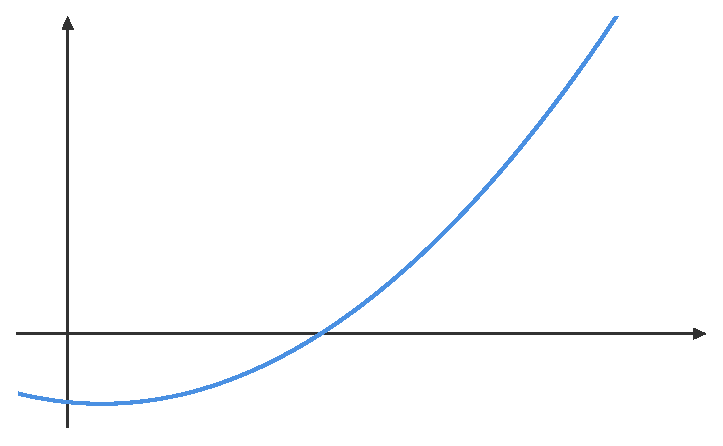
\includegraphics[width=330.75pt,height=197.25pt]{images/image_newton_method}};
%Straight Lines [id:da6424929768444043] 
\draw [color={rgb, 255:red, 155; green, 155; blue, 155 }  ,draw opacity=1 ][line width=0.75]  [dash pattern={on 4.5pt off 4.5pt}]  (510.1,106.5) -- (510.1,284.5) ;
%Straight Lines [id:da8758554517093697] 
\draw [color={rgb, 255:red, 155; green, 155; blue, 155 }  ,draw opacity=1 ]   (510.1,105.5) -- (382,289.33) ;
%Straight Lines [id:da8632115968328404] 
\draw [color={rgb, 255:red, 155; green, 155; blue, 155 }  ,draw opacity=1 ][line width=0.75]  [dash pattern={on 4.5pt off 4.5pt}]  (382,262.5) -- (382,285.33) ;
%Straight Lines [id:da10976638691733442] 
\draw [color={rgb, 255:red, 155; green, 155; blue, 155 }  ,draw opacity=1 ]   (340.5,289.5) -- (382,253.2) ;
%Straight Lines [id:da28590987584360095] 
\draw    (510.1,289.5) -- (510.1,293.2) ;
%Straight Lines [id:da06729921605109834] 
\draw    (510.1,286) -- (510.1,290) ;
%Straight Lines [id:da18775137309121925] 
\draw [color={rgb, 255:red, 155; green, 155; blue, 155 }  ,draw opacity=1 ]   (518.35,93.95) -- (510.1,105.5) ;
%Shape: Circle [id:dp7916165248356848] 
\draw  [fill={rgb, 255:red, 255; green, 255; blue, 255 }  ,fill opacity=1 ] (508.1,105.5) .. controls (508.1,104.4) and (509,103.5) .. (510.1,103.5) .. controls (511.2,103.5) and (512.1,104.4) .. (512.1,105.5) .. controls (512.1,106.6) and (511.2,107.5) .. (510.1,107.5) .. controls (509,107.5) and (508.1,106.6) .. (508.1,105.5) -- cycle ;
%Straight Lines [id:da1316603229735085] 
\draw    (382,289.5) -- (382,293.2) ;
%Straight Lines [id:da9560432424659024] 
\draw    (340.5,289.5) -- (340.5,293.2) ;
%Straight Lines [id:da2626747830873235] 
\draw    (382,286) -- (382,290) ;
%Straight Lines [id:da9507317011882577] 
\draw    (340.5,285.5) -- (340.5,289.5) ;
%Straight Lines [id:da6325259503800027] 
\draw [color={rgb, 255:red, 155; green, 155; blue, 155 }  ,draw opacity=1 ]   (382,253.2) -- (423.5,216.9) ;
%Shape: Circle [id:dp23034405156952054] 
\draw  [fill={rgb, 255:red, 255; green, 255; blue, 255 }  ,fill opacity=1 ] (380,253.2) .. controls (380,252.1) and (380.9,251.2) .. (382,251.2) .. controls (383.1,251.2) and (384,252.1) .. (384,253.2) .. controls (384,254.3) and (383.1,255.2) .. (382,255.2) .. controls (380.9,255.2) and (380,254.3) .. (380,253.2) -- cycle ;
%Straight Lines [id:da641645989007537] 
\draw [color={rgb, 255:red, 155; green, 155; blue, 155 }  ,draw opacity=1 ]   (526.6,82.4) -- (518.35,93.95) ;

% Text Node
\draw (162,68.4) node [anchor=north west][inner sep=0.75pt]  [font=\footnotesize]  {$f( x)$};
% Text Node
\draw (503.5,298.4) node [anchor=north west][inner sep=0.75pt]  [font=\footnotesize]  {$x_{0}$};
% Text Node
\draw (375.5,298.4) node [anchor=north west][inner sep=0.75pt]  [font=\footnotesize]  {$x_{1}$};
% Text Node
\draw (585,285.4) node [anchor=north west][inner sep=0.75pt]  [font=\footnotesize]  {$x$};
% Text Node
\draw (334,298.4) node [anchor=north west][inner sep=0.75pt]  [font=\footnotesize]  {$x_{2}$};
% Text Node
\draw (524,106) node [anchor=north west][inner sep=0.75pt]  [font=\footnotesize,color={rgb, 255:red, 155; green, 155; blue, 155 }  ,opacity=1 ] [align=left] {Curve tangent\\at point $\displaystyle x_{0}$.};
% Text Node
\draw (304,209) node [anchor=north west][inner sep=0.75pt]  [font=\footnotesize,color={rgb, 255:red, 155; green, 155; blue, 155 }  ,opacity=1 ] [align=left] {Curve tangent\\at point $\displaystyle x_{1}$.};


\end{tikzpicture}


	\caption{Newton-Raphson method to approximate the zero crossing of a function.}
	\label{fig:tikz_newton_method}
\end{figure}
The approximation quality of the zero crossing $x_R$ can be determined with the specified precision $\left| x_{n + 1} - x_n \right| < \varepsilon$. In order for the algorithm to converge towards the zero crossing, the start value $x_0$ must be found accordingly.

Based on the previous findings, the elements of the vector of zero crossings $\mathrm{\mathbf{x}} = \mathrm{\mathbf{x}}_R$ of the vector of functions $\mathrm{\mathbf{f}} \left( \mathrm{\mathbf{x}} \right) : \mathbb{R}^m \to \mathbb{R}^m$ with $m \in \mathbb{N}$, for which $\mathrm{\mathbf{f}}\left( \mathrm{\mathbf{x}}_R \right) = \mathbf{0}$ applies, can be approximated as shown below.
\begin{center}
	\begin{equation} \label{eq:vect_x_approx}
		\mathrm{\mathbf{x}}_{R, n + 1} = \mathrm{\mathbf{x}}_{R,n} 	- \mathrm{\mathbf{J}}^{-1}\left( \mathrm{\mathbf{x}}_{R,n} \right) \, \mathrm{\mathbf{f}}\left( \mathrm{\mathbf{x}}_{R,n} \right) 
	\end{equation}
\end{center}
The Jacobian matrix $\mathrm{\mathbf{J}}$ contains all partial derivatives of the function vector with respect to the vector of the zero crossings.
\begin{center}
	\begin{equation} \label{eq:jacobian}
		\mathrm{\mathbf{J}} = \left. \dfrac{\partial \mathrm{\mathbf{f}}\left(\mathrm{\mathbf{x}}\right)}{\partial \mathrm{\mathbf{x}}} \right|_{\mathrm{\mathbf{x}} = \mathrm{\mathbf{x}}_R} = 
 		\begin{pmatrix}
  			\dfrac{\partial}{\partial x_1} f_1\left( \mathrm{\mathbf{x}}_R \right) & \dfrac{\partial}{\partial x_2} f_1\left( \mathrm{\mathbf{x}}_R \right) & \cdots & \dfrac{\partial}{\partial x_m} f_1\left( \mathrm{\mathbf{x}}_R \right) \\
			\dfrac{\partial}{\partial x_1} f_2\left( \mathrm{\mathbf{x}}_R \right) & \dfrac{\partial}{\partial x_2} f_2\left( \mathrm{\mathbf{x}}_R \right) & \cdots & \dfrac{\partial}{\partial x_m} f_2\left( \mathrm{\mathbf{x}}_R \right) \\
			\vdots & \vdots & \ddots & \vdots \\
  			\dfrac{\partial}{\partial x_1} f_m\left( \mathrm{\mathbf{x}}_R \right) & \dfrac{\partial}{\partial x_2} f_m\left( \mathrm{\mathbf{x}}_R \right) & \cdots & \dfrac{\partial}{\partial x_m} f_m\left( \mathrm{\mathbf{x}}_R \right) 
 		\end{pmatrix}
 	\end{equation}
\end{center}
For completeness it is noted that $ \mathrm{\mathbf{x}}_R = \big( x_1, \dotsc, x_m \big)^{\mathrm T } $ does not correspond to the figure \ref{fig:tikz_newton_method}. The elements $x_1$ to $x_m$ of the vector $\mathrm{\mathbf{x}}_R$ are zero crossings of the functions contained by the vector $\mathrm{\mathbf{f}} \left( \mathrm{\mathbf{x}}_R \right) = \big( f_1\left( \mathrm{\mathbf{x}}_R \right), \dotsc, f_m\left( \mathrm{\mathbf{x}}_R \right) \big)^{\mathrm T } = \mathbf{0}$. Their $\left(n + 1\right)$\textsuperscript{th} approximation is $\mathrm{\mathbf{x}}_{R,n + 1} = \big( x_{1,n + 1}, \dotsc, x_{m,n + 1} \big)^{\mathrm T}$.


\chapter{\altmatlab and \altmaple source codes} \label{sec:matlab_source_codes}
This appendix contains the \MATLAB simulation which was used to simulate the self-sufficient energy distribution system and the \MAPLE source code which was used to calculate the Jacobian matrix in the subsection \ref{sec:photovoltaic_generators}. 

\section{\altmatlab simulation of the self-sufficient energy distribution system} \label{sec:matlab_code}
\begin{lstlisting}
%% MAIN: Self-sufficient energy distribution system performance estimation
% This simulation provides a performance estimation of the self-sufficient energy distribution system, which is part of the voice communication system of the OeWF Serenity spacesuit simulator. It can be simulated if the repeater radio infrastructure can operate at a certain mission location on Earth. All sections labeled [INPUT] can be manipulated. For further information please refer to the MATLAB documentation, look into the bachelor thesis about this simulation or contact the author.

% Organization:     OeWF (Austrian Space Forum)
% Author:           Omar Filip El Sendiouny
% Project:          Serenity BU-COMMs
% Date:             15.12.2020
% Version:          1 

clear all;
close all;
clc;

show_command_window_output = 1; % allow command window output
N_dp = 4; % number of decimal points for solar angle calculations (accuracy)

dfile ='command_window_output.txt'; % command window output can be found in the local folder
if(exist(dfile, 'file'))
    delete(dfile); 
end
diary(dfile)
diary on

%% [INPUT] Mission information:
% It it assumed that the missions start at the same time every day for the entire duration of the mission. The time of the mission start must be smaller than the time of mission end.

lat = 30.500; % latitude in (deg)
lon = 35.917; % longitude in (deg)
irradiation_GH = 6.05; % daily total of the global horizontal irradiation in (kWh / m^2) 
irradiation_DN = 6.85; % daily total of the direct normal irradiation in (kWh / m^2)
date(1) = datetime(2021, 10, 4); % mission start date in (Y, M, D)
date(2) = datetime(2021, 10, 31); % mission end date in (Y, M, D)
t_UTC(1) = {'4:00'}; % time of the daily mission start in (h)
t_UTC(2) = {'14:00'}; % time of the daily mission end in (h)
ALB = 0.30; % albedo in (1)
theta_A = 22.3; % average ambient temperature in (degrees C)

%% [INPUT] Photovoltaic generator:
% MPP ... maximim power point
% STC ... standard test conditions
% SC ... short-circuit
% OC ... open-circuit

N_C = 36; % number of PV cells in (1)
A_PV = 0.88; % PV generator area in (m^2)
I_MPP_STC = 9.11; % current at MPP for STC in (A)
U_MPP_STC = 21.41; % voltage at MPP for STC in (V)
I_SC_STC = 9.79; % SC current for STC in (A)
U_OC_STC = 24.27; % OC voltage for STC in (V)
TC_I_SC = 0.05; % temperature coefficient for I_SC in (% / degC)
TC_U_OC = -0.29; % temperature coefficient for U_OC in (% / degC)
NOCT = 45; % nominal operating cell temperature in (degC)
m = 1.19045; % ideality factor in (1)
N_PV = 1; % number of PV generators (if greater than 1, they are connected in parallel)

%% [IMPUT] Load (repeater radio system):
% After t_UTC(2) and before t_UTC(1) the repeater radio system is in standby. The sum of the duty cycles must be 100%.

U_L_min = 11.0; % minimum load voltage in (V)
U_L_max = 15.5; % maximum load voltage in (V)
I_T = 3; % current consumption when the load transmits in (A)
I_R = 0.7; % current consumption when the load receives in (A)
I_Stby = 0.7; % current consumption when the load is in standby in (A)
a_T = 20; % duty cycle when transmitting in (%) 
a_R = 20; % duty cycle when receiving in (%)
a_Stby = 60; % duty cycle when in standby in (%)
I_add = 0; % additional load current in (A)

%% [INPUT] LiFePo_4 battery
% The initial state of charge of the battery is usually the SOC for storage, which is between 50% and 60%.

SOC_init = 0.6; % initial state of charge in (1)
Q_nom = 50; % nominal charge in (Ah)
C_D = 1/3; % discharging rate for Q_nom in (h^(-1))

% Obtained from the discharging an charging experiments:
SOC = [1.00 0.95 0.90 0.85 0.80 0.75 0.70 0.65 0.60 0.55 0.50 0.45 0.40 0.35 0.30 0.25 0.20 0.15 0.10 0.05 0.00]; % state of charge in (1) of the battery
U_0_D = [13.877 13.315 13.319 13.322 13.320 13.306 13.248 13.196 13.181 13.117 13.174 13.172 13.169 13.111 13.087 13.012 12.931 12.837 12.814 12.350 11.371]; % open-circuit voltages when discharging the battery in (V)
U_0_C = [14.107 13.387 13.393 13.401 13.415 13.388 13.387 13.275 13.272 13.253 13.250 13.248 13.250 13.244 13.225 13.179 13.089 12.958 12.923 12.502 11.420]; % open-circuit voltages when charging the battery in (V)
R_e_D = [0.0120840740086789 0.0117154203104446 0.0117700588020157 0.0117132299485587 0.0116221338950336 0.0116467701188540 0.0116605558931997 0.0115638462618863 0.0116222251883952 0.0116974390402753 0.0116987272047564 0.0117465274490441 0.0117588908671468 0.0117566064015986 0.0117756658545291 0.0117553658832641 0.0117583775845481 0.0117768748688630 0.0117155094645921 0.0118414656950463 0.0120957986167104]; % electrolyte resistances when discharging in (Ohm)
R_e_C = [0.0121012406947893 0.0113356302935661 0.0114597641410590 0.0114014839745851 0.0114900762492556 0.0116012192457450 0.0112273867826839 0.0112396239841211 0.0111117629249463 0.0112231518757464 0.0113202903133204 0.0112805170265242 0.0114125559543423 0.0114503161497776 0.0114125257730806 0.0115293500897879 0.0115664251765242 0.0115250208156497 0.0117012683150631 0.0118226401014494 0.0120662511263975]; % electrolyte resistances when charging in (Ohm)

%% [INPUT] Solar charging controller
% The SCC only connects the PV generator when its voltage at the PV generator input terminal exceeds U_Bat + 5V. As soon as this condition is met the PV generator remains connected as long as the voltage at the PV generator input terminal is greater than U_Bat + 1V.

I_SCC = 0.020; % current consumption of the SCC in (A)
I_B_max = 10; % maximum battery current in (A)
P_MPP_max = 145; % maximum power from PV generator in (W)
eta_SCC = 0.98; % efficiency in (1)

%% [INPUT] Cables:
% Only one wire of the cable is to be described. For more information, please refer to the subsection 3.1.2 (Repeater radio infrastructure) of the bachelor thesis about this simulation.

% Input sytle: cables = [cable_A; cable_B; cable_C]
% Input style: cables(n,:) = [length cross_section_area specific_resistance temperature_coefficient]

% length in (m)
% cross_section_area in (mm^2)
% specific_resistance for 20 degC in (Ohm * mm^2 / m)
% temperature coefficientc for 20 degC in (degC^(-1))

cables = [0.9 4.0 0.01673 4.3 * 10^(-3); 0.5 4.0 0.01673 4.3 * 10^(-3); ...
    11.0 2.5 0.01673 4.3 * 10^(-3)];  

%% [OUTPUT] Radiation flux received by an inclined PV generator:
% To ensure better readability, for-loops were used instead of direct assignments for most vectors/matrices. This further helps with the maintenance of the program. However, it decreases the performance of the simulation (fix in version 1.1)

lat = round(lat, N_dp);
lon = round(lon, N_dp);

date_array = (date(1):date(2))'; % contains all mission dates
N_md = split(between(date(1), date(2), 'days'), 'days') + 1; % number of mission days

delta_t_S = 0.01; % resolution for solar time
N_dp_delta_t_S = 0; % number of decimal places of delta_t_S

while (floor(delta_t_S * 10^N_dp_delta_t_S) ~= delta_t_S * 10^N_dp_delta_t_S) % find the number of decimal places of delta_t_S
N_dp_delta_t_S = N_dp_delta_t_S + 1;
end

t_S = round(0:delta_t_S:24, N_dp_delta_t_S); % solar time
h_S = round((t_S - 12) * 15, N_dp); % solar hour angle

N_d = zeros(N_md, 1); % number of days since Jan. 1st
delta = zeros(N_md, 1); % Sun declination
beta = zeros(N_md, 1); % optimal inclination angle for the PV generator
h_rs = zeros(N_md, 2); % solar sunrise and sunset hour angles

for n = 1:N_md % calculating N_d, delta, and beta
    N_d(n) = 30.3 * (month(date_array(n)) - 1) + day(date_array(n));
    delta(n) = round(23.45 * sind((360 * (284 + N_d(n)) / 365)), N_dp);
    beta(n) = round(abs(lat - delta(n)), N_dp);
end

beta_mean = mean(beta); % mean value of beta will be used from now on

for n = 1:N_md % calculating h_rs
    if(abs(lat) < 90 - abs(delta(n)))
        h_rs(n,1) = round(- acosd(- tand(delta(n)) * tand(lat)), N_dp); % solar sunrise hour angle
        h_rs(n,2) = round(- h_rs(n,1), N_dp); % solar sunset hour angle
    else
        error('Solar sunrise and sunset angles cannot not be calculated!');
    end
end

t_rs = 12 + h_rs / 15; % solar sunrise and sunrise times

idx = h_S <= 0; % get index for solar hour angles from t_S = 0h to t_S = 12h
h_S_fhd = h_S(idx); % create associated vector for solar hour angles (first half of the day)

gamma_S = zeros(N_md, length(h_S_fhd)); % altitude of the Sun
alpha_S = zeros(N_md, length(h_S_fhd)); % azimuth of the Sun
theta = zeros(N_md, length(h_S_fhd)); % angle theta (solar incidence angle)

for n = 1:N_md % calculating gamma_S_deg from sunrise to t_S = 12h
    for o = 1:length(h_S_fhd)
        if(h_S_fhd(o) >= h_rs(n,1)) % if the Sun is above the horizon
            gamma_S(n,o) = round(asind(sind(lat) * sind(delta(n)) + cosd(lat) * cosd(delta(n)) * cosd(h_S_fhd(o))), N_dp); 
         else
            gamma_S(n,o) = NaN; % invalid angle (Sun is below the horizon)
        end
    end
end

for n = 1:N_md % calculating alpha_S_deg from sunrise to t_S = 12h
    for o = 1:length(h_S_fhd)
        if(h_S_fhd(o) >= h_rs(n,1) && h_S_fhd(o) ~= 0) % if the Sun is above the horizon before t_S = 12h
            alpha_S(n,o) = round(-acosd((sind(lat) * cosd(delta(n)) * cosd(h_S_fhd(o)) - cosd(lat) * sind(delta(n))) / cosd(gamma_S(n,o))), N_dp); 
        elseif(h_S_fhd(o) == 0 && gamma_S(n,o) ~= 90) % if t_S = 12h and the Sun is not at its zenith
            if(lat > delta(n))
                alpha_S(n,o) = round(0, N_dp);
            elseif(lat < delta(n))
                alpha_S(n,o) = round(180, N_dp);
            end
        else % the Sun is below the horizon or at its zenith
            alpha_S(n,o) = NaN; % invalid angle
        end  
    end
end

for n = 1:N_md % calculating theta
    for o = 1:length(h_S_fhd)
        if(h_S_fhd(o) >= h_rs(n,1)) % if the Sun is above the horizon
            if(gamma_S(n,t_S == 12) ~= 90) % if the Sun is not at its zenith
                tmp = sind(delta(n)) * sind(lat) * cosd(beta_mean) ...
                    - sind(delta(n)) * cosd(lat) * sind(beta_mean) * cosd(alpha_S(n, t_S == 12)) ...
                    + cosd(delta(n)) * cosd(lat) * cosd(beta_mean) * cosd(h_S_fhd(o)) ...
                    + cosd(delta(n)) * sind(lat) * sind(beta_mean) * cosd(alpha_S(n,o)) * cosd(h_S_fhd(o)) ...
                    + cosd(delta(n)) * sind(beta_mean) * sind(alpha_S(n, t_S == 12)) * cosd(h_S_fhd(o));
                if(tmp>1) % necessary because of rounding errors caused by matlab
                    tmp = 1;
                end 
                    theta(n,o) = round((acosd(tmp)), N_dp);      
            elseif(gamma_S(n,t_S == 12) == 90) % if the Sun is at its zenith
                tmp = sind(delta(n)) * sind(lat) ... 
                    + cosd(delta(n)) * cosd(lat) * cosd(h_S_fhd(o));
                theta(n,o) = round(acosd(tmp), N_dp);
            end
        else
            theta(n,o) = NaN; % invalid angle
        end
    end
end

for n = 1:N_md % because of the projection of the normal to A_PV onto plane earth?
    [~, idx(n)] = max(theta(n,:));
    for o = 1:length(theta)
        if(o < idx(n) || theta(n,o) >= 90.0) % if the Sun's rays do not hit A_PV
            theta(n,o) = NaN;
        end
    end
end

tmp_mat = gamma_S;
tmp_mat = fliplr(tmp_mat); % flip the temporary matrix from left to right
tmp_mat(:,1) = []; % delete first entry so it does not appear twice in the gamma_S matrix
gamma_S = [gamma_S tmp_mat]; % allowed because the Sun is symmetrical around t_S = 12h

tmp_mat = alpha_S;
tmp_mat = fliplr(tmp_mat); % flip the temporary matrix from left to right
tmp_mat(:,1) = []; % delete first entry so it does not appear twice in the alpha_S matrix
alpha_S = [alpha_S -tmp_mat]; % allowed because the Sun is symmetrical around t_S = 12h

tmp_mat = theta;
tmp_mat = fliplr(tmp_mat); % flip the temporary matrix from left to right
tmp_mat(:,1) = []; % delete first entry so it does not appear twice in the theta matrix
theta = [theta tmp_mat]; % allowed because the Sun is symmetrical around t_S = 12h

E_GHI = irradiation_GH * 10^(3) / 24; % global horizontal irradiance 
E_DNI = irradiation_DN * 10^(3) / 24; % direct normal irradiance

E_G = zeros(N_md, length(t_S)); % total irradiance received by an inclined PV generator
W_G = zeros(N_md, 1); % solar energy yield
tau_S = zeros(N_md, 1); % auxiliary variable
Phi_max = zeros(N_md, 1); % maximal daily radiation flux
Phi_G = zeros(N_md, length(t_S)); % radiation flux received by an inclined PV generator 

for n = 1:N_md % calculating E_G
    for o = 1:length(t_S)
        if(isnan(theta(n,o)) && ~isnan(gamma_S(n,o)))
            E_G(n,o) = (E_GHI - E_DNI * sind(gamma_S(n,o))) * (1 + cosd(beta_mean)) / 2; % PV generator receives DIFG
        elseif(~isnan(theta(n,o)) && ~isnan(gamma_S(n,o))) % PV generator receives DGI, DIFG and RGI
            E_G(n,o) = E_DNI * cosd(theta(n,o)) ...
                + (E_GHI - E_DNI * sind(gamma_S(n,o))) * (1 + cosd(beta_mean)) / 2 ...
                + E_GHI * ALB * (1 - cosd(beta_mean)) / 2;
        else
            E_G(n,o) = 0;
        end
    end
end

for n = 1:N_md % calculating W_G
    for o = 1:length(t_S)
        W_G(n) = W_G(n) + A_PV * E_G(n,o) * delta_t_S;
    end
end

for n = 1:N_md % calculating Phi_G
    for o = 1:length(t_S)
        tau_S(n) = (12 - t_rs(n,1)) / 3;
        Phi_max(n) = 0.997 / (tau_S(n) * sqrt(2 * pi)) * W_G(n);
        Phi_G(n,o) = Phi_max(n) * exp(- (t_S(o) - 12)^2/(2 * tau_S(n)^2));
    end
end
 
%% [OUTPUT] PV generator power output

e = 1.602176634 * 10^(-19); % elementary charge in (As)
k_B = 1.380649 * 10^(-23); % Bolzmann constant in (Ws/K)

theta_C = zeros(N_md, length(t_S)); % PV cell temperature
U_T = zeros(N_md, length(t_S)); % thermal voltage
I_Ph = zeros(N_md, length(t_S)); % photocurrent
I_Ph_irr_STC = zeros(N_md, length(t_S)); % photocurrent with E_STC
U_OC_0 = zeros(N_md, length(t_S)); % open-circuit voltage
I_S_0 = zeros(N_md, length(t_S)); % reverse saturation current

for n = 1:N_md % calculating the parameters initialized above
    for o = 1:length(t_S)
        theta_C(n,o) = theta_A + (NOCT - 20) * Phi_G(n,o) * A_PV / 800;
        U_T(n,o) = k_B * (theta_C(n,o) + 273.15)/e;
        I_Ph(n,o) = I_SC_STC * Phi_G(n,o) * A_PV * (1 + TC_I_SC / 100 * (theta_C(n,o) - 25)) / 1000;
        I_Ph_irr_STC(n,o) = I_SC_STC * (1 + TC_I_SC / 100 * (theta_C(n,o) - 25));
        U_OC_0(n,o) = U_OC_STC * (1 + TC_U_OC / 100 * (theta_C(n,o) - 25)) ...
            + m * N_C * U_T(n,o) * log(I_Ph(n,o) / I_Ph_irr_STC(n,o));
        
        if(U_OC_0(n,o) < 0) % so that I_S << I_Ph is fulfilled
            U_OC_0(n,o) = NaN;
            I_S_0(n,o) = NaN;
        else
            I_S_0(n,o) = I_Ph(n,o) * exp(- (U_OC_0(n,o)) / (m * N_C * U_T(n,o)));
        end
    end
end

[idxn, idxo] = find(U_OC_0 == max(max(U_OC_0))); % finding maximum value in U_OC_0 matrix (improve in version 1.1)
delta_U_PV = 0.01; % resolution for PV generator voltage
U_PV = 0:delta_U_PV:U_OC_0(idxn,idxo) + delta_U_PV; % PV generator voltage
I_PV = zeros(N_md, length(t_S), length(U_PV)); % PV generator current
P_PV = zeros(N_md, length(t_S), length(U_PV)); % PV generator power
P_MPP = zeros(N_md, length(t_S)); % PV generator power for MPP
U_MPP = zeros(N_md, length(t_S)); % PV generator voltage for MPP
I_MPP = zeros(N_md, length(t_S)); % PV generator current for MPP
W_G_el = zeros(N_md, 1); % electrical energy yield of the PV generator

for n = 1:N_md % caluculating PV generator current and MPP values as well as its daily electrical energy yield (3D matrix ... noice UwU)
    for o = 1:length(t_S)
        for p = 1:length(U_PV)
            I_PV(n,o,p) = N_PV * (I_Ph(n,o) - I_S_0(n,o) * (exp(U_PV(p)/(m * N_C * U_T(n,o))) - 1));
            
            if(I_PV(n,o,p) < 0)
                I_PV(n,o,p) = NaN;
            end
            
            P_PV(n,o,p) = I_PV(n,o,p) * U_PV(p);
            
            if(isnan(P_PV(n,o,p)))
                P_PV(n,o,p) = 0;
            end
        end
        
        [P_MPP(n,o), idx] = max(P_PV(n,o,:));
        U_MPP(n,o) = U_PV(idx);
        
        if(isnan(I_PV(n,o,idx)))
            I_MPP(n,o) = 0;
        else
            I_MPP(n,o) = I_PV(n,o,idx);
        end
    end
end

for n = 1:N_md % calculating W_G_el
    for o = 1:length(t_S)
        W_G_el(n) = W_G_el(n) + P_MPP(n,o) * delta_t_S; % electrical energy yield
    end
end

%% [OUTPUT] Load (repeater radio system)
% The load current is an average current, because an on-off step function could not be implemented.

dtv = datevec(datetime(t_UTC{1},'InputFormat','HH:mm')); % converitng time of daily mission start to floating point number
da = duration(dtv(:,4:end));
t_UTC_float(1) = hours(da);

dtv = datevec(datetime(t_UTC{2},'InputFormat','HH:mm')); % converitng time of daily mission end to floating point number
da = duration(dtv(:,4:end));
t_UTC_float(2) = hours(da);

Z_h = zeros(N_md, 1); % equation of time 
t_S_mission_se = zeros(N_md, 2); % solar mission start and end times
I_L = zeros(N_md, length(t_S)); % load current

for n = 1:N_md % calculating solar mission time
    Z_h(n) = 0.123 * cosd(360 * (88 + N_d(n)) / 365) - 0.167 * sind(720 * (10 + N_d(n)) / 365);
    t_S_mission_se(n, 1) = round(t_UTC_float(1) + Z_h(n) + lon / 15, N_dp_delta_t_S);
    t_S_mission_se(n, 2) = round(t_UTC_float(2) + Z_h(n) + lon / 15, N_dp_delta_t_S);
end

idx_mission_se = zeros(N_md, 2); % indices for daily mission start and end in t_S

for n = 1:N_md % find index of daily mission start and end in t_S
    [~,idx_mission_se(n,1)] = find(t_S == t_S_mission_se(n,1));
    [~,idx_mission_se(n,2)] = find(t_S == t_S_mission_se(n,2)); 
end

for n = 1:N_md % calculating I_L
    if(n == 1)
        for o = 1:length(t_S) % first day begins at mission start
            if(o < idx_mission_se(n,1))
                I_L(n,o) = 0;
            elseif(o >= idx_mission_se(n,1) && o <= idx_mission_se(n,2))
                I_L(n,o) = I_T * a_T / 100 + I_R * a_R / 100 + I_Stby * a_Stby / 100 + I_add;
            else
                I_L(n,o) = I_Stby + I_add;
            end
        end
    else
        for o = 1:length(t_S) % all other days
            if(o >= idx_mission_se(n,1) && o <= idx_mission_se(n,2))
                I_L(n,o) = I_T * a_T / 100 + I_R * a_R / 100 + I_Stby * a_Stby / 100 + I_add;
            else
                I_L(n,o) = I_Stby + I_add;
            end
        end
    end    
end

%% [OUTPUT] Cables losses

sz = size(cables);
R_wires = zeros(sz(1),1); % wire resistances

for p = 1:sz(1) % calculate all wire resistances
    R_wires(p) = cables(p,1) * cables(p,3) * (1 + cables(p,4) * (theta_A - 20)) ... 
        / cables(p,2);
end

%% [OUTPUT] Solar charging controller and LiFePO_4 battery

k_P = 1.05; % Peukert constant in (1)
I_nom = C_D * Q_nom; % nominal battery current

U_in = zeros(N_md, length(t_S)); % voltage at PV generator input terminal
U_L = zeros(N_md, length(t_S)); % voltage at repeater
Q_B = zeros(N_md, length(t_S)); % battery charge
I_B = zeros(N_md, length(t_S)); % battery current
U_B = zeros(N_md, length(t_S)); % battery voltage
SOC_curr = zeros(N_md, length(t_S)); % current state of charge of the battery
thd = 0; % threshold counter for U_MPP

delta_ip = -0.01;

SOC_ip = 1:delta_ip:0; % interpolated state of charge of the battery
U_0_D_ip = interp1(SOC, U_0_D, SOC_ip); % interpolated open-circuit voltage of the battery when discharging
U_0_C_ip = interp1(SOC, U_0_C, SOC_ip); % interpolated open-circuit voltage of the battery when charging
R_e_D_ip = interp1(SOC, R_e_D, SOC_ip); % interpolated electrolyte resistance of the battery when discharging
R_e_C_ip = interp1(SOC, R_e_C, SOC_ip); % interpolated electrolyte resistance of the battery when charging

U_0 = (U_0_D_ip + U_0_C_ip) / 2; % mean open circuit voltage

for n = 1:N_md % SCC limits power
    for o = 1:length(t_S)
        if(P_MPP(n,o) > P_MPP_max)
            P_MPP(n,o) = P_MPP_max;
            I_MPP(n,o) = P_MPP(n,o) / U_MPP(n,o);
        end
    end
end

for n = 1:N_md % PV voltage at SCC input terminal after cable losses
    for o = 1:length(t_S)
       U_in(n,o) = U_MPP(n,o) - 2 * (R_wires(1) + R_wires(2)) * I_MPP(n,o);
    end
end

[~,idx_SOC] = min(abs(SOC_ip - SOC_init)); % find closest index

for n = 1:N_md % calculating SOC and voltage of the battery (improve in version 1.1)
   for o = 1:length(t_S)
        if(n == 1 && o < idx_mission_se(n,1)) % mission on the first day has not started yet 
            thd = -1;
        elseif(n == 1 && o == idx_mission_se(n,1)) % if the mission day starts at 0:00
            if(U_in(n,o) > (U_0(idx_SOC) + 5) && (thd == 0 || thd == -1)) % I_MPP on
                thd = 1;
            elseif(U_in(n,o) < (U_0(idx_SOC) + 1) && thd == 1) % I_MPP off;
                thd = 0;
            end
        else
            if(o - 1 == 0) % if a new day started, get U_B from the last time entry from the previous day
                if(U_in(n,o) > (U_B(n - 1,length(t_S)) + 5) && (thd == 0 || thd == -1)) % I_MPP on
                    thd = 1;
                elseif(U_in(n,o) < (U_B(n - 1,length(t_S)) + 1) && thd == 1) % I_MPP off;
                    thd = 0;
                end
            else % get U_B from the same day but from the previous time entry
                if(U_in(n,o) > (U_B(n,o - 1) + 5) && (thd == 0 || thd == -1)) % I_MPP on
                    thd = 1;
                elseif(U_in(n,o) < (U_B(n,o - 1) + 1) && thd == 1) % I_MPP off;
                    thd = 0;
                end
            end 
        end
        
        if(thd == 1) % PV generator is connected (improve in version 1.1)
            I_B(n,o) =  I_SCC - I_MPP(n,o) * eta_SCC + I_L(n,o);
        elseif(thd == 0) % PV generator is disconnected
            I_B(n,o) =  I_SCC + I_L(n,o);
        elseif(thd == -1) % before the mission starts on the first day
            I_B(n,o) = 0;
        end
        
        if(I_B(n,o) > I_B_max)
            I_B(n,o) = I_B_max;
        elseif(I_B(n,o) < - I_B_max)
            I_B(n,o) = - I_B_max;
        end
        
        if(I_B(n,o) > 0) % battery is discharging 
            Q_tot = Q_nom * (I_nom / I_B(n,o))^(k_P - 1);
            
            if(n > 1 && o == 1) % get SOC from the end of the previous day
                SOC_curr(n,o) = SOC_curr(n - 1, length(t_S)) - (1 / Q_tot) * I_B(n,o) * delta_t_S;
            else % get previous state of charge
                SOC_curr(n,o) = SOC_curr(n,o - 1) - (1 / Q_tot) * I_B(n,o) * delta_t_S;
            end
            
            if(SOC_curr(n,o) > 1)
                SOC_curr(n,o) = 1;
            elseif(SOC_curr(n,o) < 0)
                SOC_curr(n,o) = 0;
            end
            
            [~,idx_SOC] = min(abs(SOC_ip - SOC_curr(n,o))); % find closest index
            c_B = abs(U_0_C_ip(idx_SOC) - U_0_D_ip(idx_SOC)) / 2;
            U_B(n,o) = U_0(idx_SOC) - c_B - R_e_D_ip(idx_SOC) * I_B(n,o);
            
        elseif(I_B(n,o) < 0) % battery is charging 
            Q_tot = Q_nom;
            
            if(n > 1 && o == 1) % get SOC from the end of the previous day
                SOC_curr(n,o) = SOC_curr(n - 1, length(t_S)) - 1 / Q_tot * I_B(n,o) * delta_t_S;
            else % get previous state of charge
                SOC_curr(n,o) = SOC_curr(n,o - 1) - 1 / Q_tot * I_B(n,o) * delta_t_S;
            end
            
            if(SOC_curr(n,o) > 1)
                SOC_curr(n,o) = 1;
            elseif(SOC_curr(n,o) < 0)
                SOC_curr(n,o) = 0;
            end
            
            [~,idx_SOC] = min(abs(SOC_ip - SOC_curr(n,o))); % find closest index
            c_B = abs(U_0_C_ip(idx_SOC) - U_0_D_ip(idx_SOC)) / 2;
            U_B(n,o) = U_0(idx_SOC) + c_B - R_e_C_ip(idx_SOC) * I_B(n,o);
            
        elseif(I_B(n,o) == 0) % battery is in standby (SOC_init stays the same)
            if(n == 1 && o == 1)
                SOC_curr(n,o) = SOC_init;
            elseif(n > 1 && o == 1) % get SOC from the end of the previous day
                SOC_curr(n,o) = SOC_curr(n - 1,length(t_S));
            else % get previous state of charge
                SOC_curr(n,o) = SOC_curr(n,o - 1);
            end
            
            if(SOC_curr(n,o) > 1)
                SOC_curr(n,o) = 1;
            elseif(SOC_curr(n,o) < 0)
                SOC_curr(n,o) = 0;
            end
            
            [~,idx_SOC] = min(abs(SOC_ip - SOC_curr(n,o))); % find closest index
            U_B(n,o) = U_0(idx_SOC);
        end 
        
        U_L(n,o) =  U_B(n,o) - 2 * R_wires(3) * I_B(n,o); % voltage at repeater after cable losses
        if(U_L(n,o) < U_L_min)
            error('Voltage at repeater radio system is too low!');
        elseif(U_L(n,o) > U_L_max)
            error('Voltage at repeater radio system is too high!');
        end
   end
end

if(min(min(SOC_curr)) == 0) % battery got fully discharged
    error('LiFePO_4 battery gets fully discharged! Use more PV generators in parallel!');
end

%% [OUTPUT] Command window and plots

fnct_cw_output(show_command_window_output, N_md, gamma_S, alpha_S, ...
    date_array, beta, t_S, W_G_el, SOC_curr); % command window output
 
diary off
\end{lstlisting}
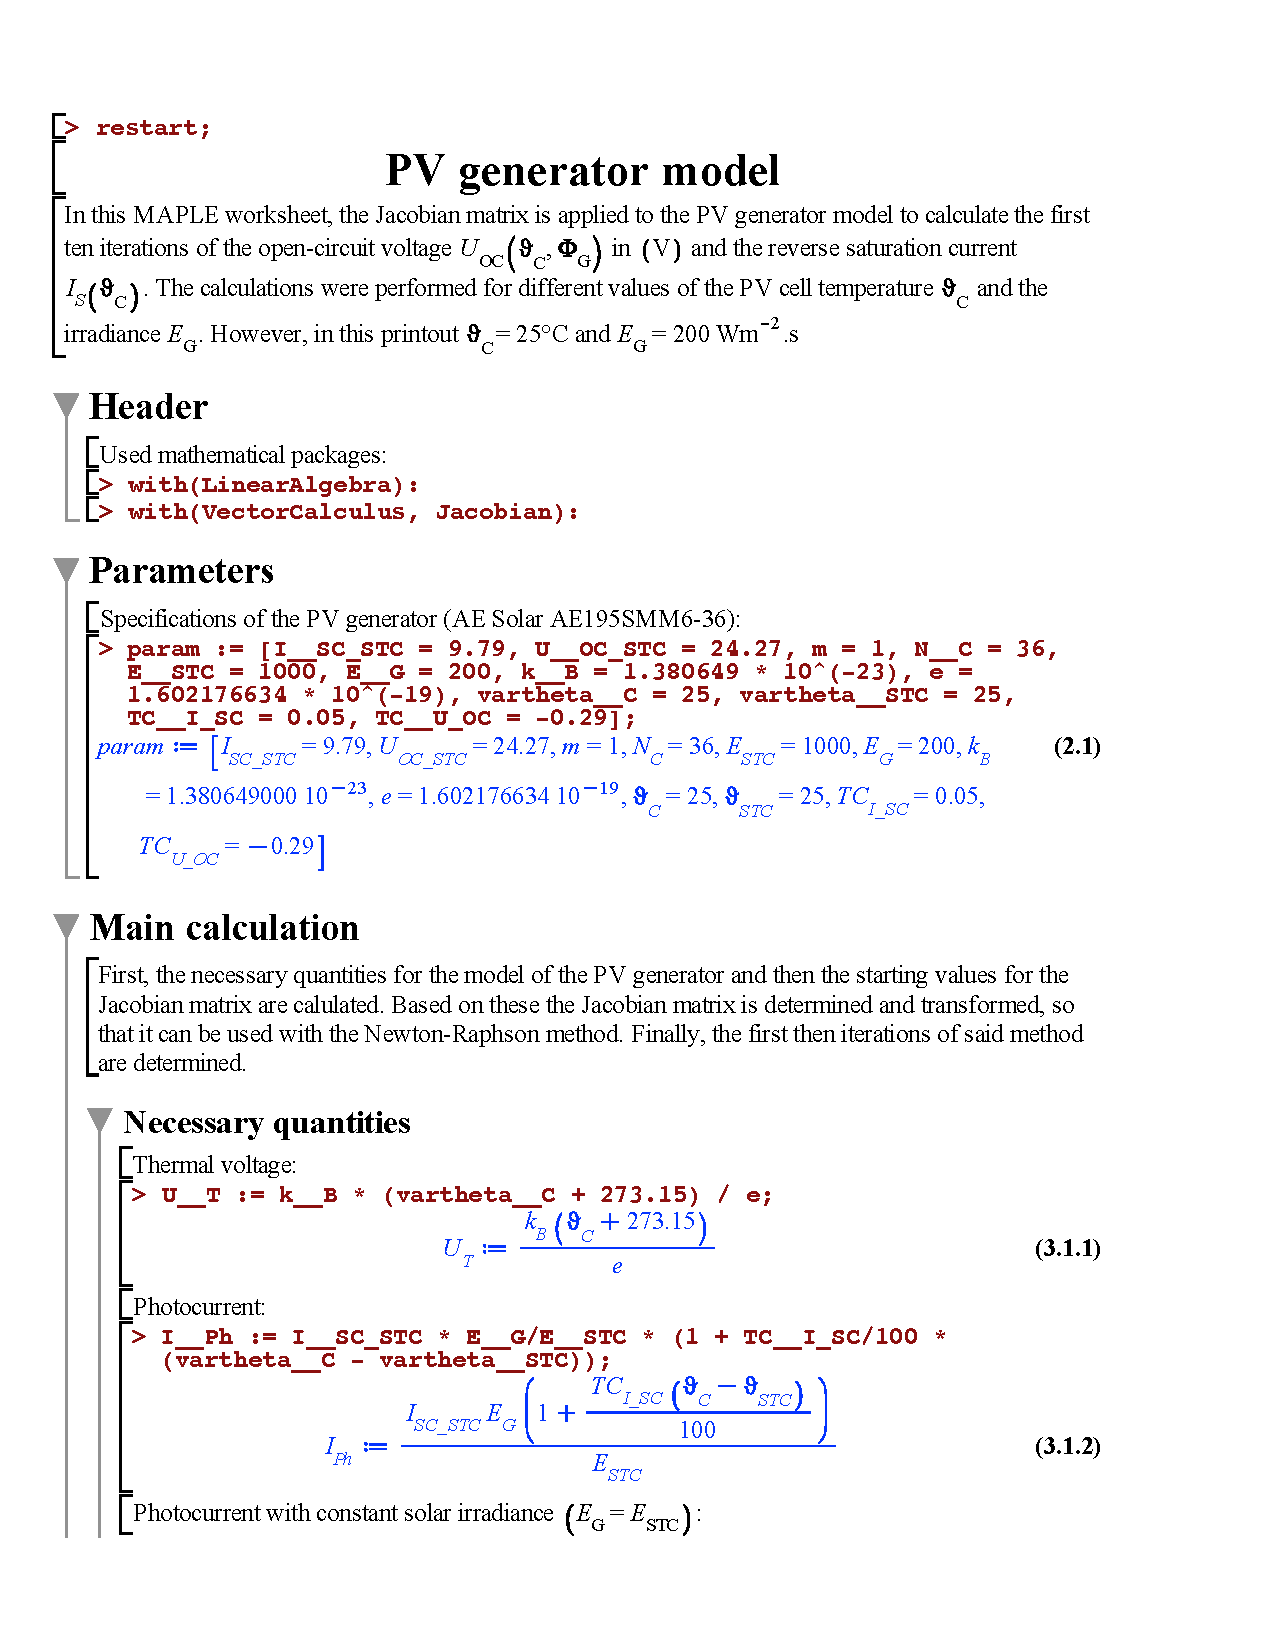
\includepdf[pages=1, pagecommand={\pagestyle{fancy}}, scale = 0.9, pagecommand=\section{\altmaple source code for the Jacobian matrix}\label{sec:maple_code}]{pdf_files/maple_code.pdf}
\includepdf[pages=2, pagecommand={\pagestyle{fancy}}, scale = 0.9]{pdf_files/maple_code.pdf}
\includepdf[pages=3, pagecommand={\pagestyle{fancy}}, scale = 0.9]{pdf_files/maple_code.pdf}

\clearpage
\pagenumbering{arabic}	% resets page numbering to 1
\renewcommand*{\thepage}{R\arabic{page}}

\fancyhead{}																% clearing all the head fields
\fancyhead[RO]{Voice communication system for a spacesuit simulator}		% RO ... Right Odd, LE ... Left Even
\fancyhead[LE]{\nouppercase{\leftmark}}										% also try \rightmark, \leftmark and \chaptermark
\fancyfoot{}
\fancyfoot[RO, LE]{\thepage}

\addcontentsline{toc}{chapter}{References}
\printbibliography[title = References]

\end{document}